\documentclass[12pt]{book}
\usepackage{graphicx}
\usepackage[dvipsnames, table]{xcolor}
\usepackage[hidelinks]{hyperref}
\usepackage{tcolorbox}
\tcbuselibrary{skins,raster,many}
\usepackage{geometry}
\usepackage{longtable}
\usepackage{float}
\usepackage{pdfpages}
\usepackage{amsmath}
\usepackage{amssymb}
\usepackage[document]{ragged2e}
\setcounter{tocdepth}{4}
\setcounter{secnumdepth}{4}
\usepackage{tablefootnote}
\usepackage{enumitem}
\usepackage[toc,titletoc,title]{appendix}
\usepackage{booktabs}
\usepackage{array}
\usepackage{multirow}
\usepackage[toc,section=chapter, acronym]{glossaries-extra}
\usepackage{wasysym}
\usepackage{CormorantGaramond}

\loadglsentries{glossary.tex}
% \loadglsentries{acronyms.tex}

% Defining the glossary for case summaries
\newglossary[slg]{summaries}{syi}{syg}{Case Summaries}

% Glossary entry for Al-Saadoon v Secretary of State for Defence
\newglossaryentry{summary:al-saadoon v sec. def}{
    type=summaries,
    name={\textit{Al-Saadoon v Secretary of State for Defence} [2010] EWCA Civ 776},
    sort={Al-Saadoon v Secretary of State for Defence},
    description={Al-Saadoon and others were detained in Iraq by British forces; the UK Court of Appeal held that the UK was bound by the Geneva Conventions, and had a duty to ensure detainees were treated in accordance with international law, including the prohibition on torture, demonstrating that regional customary norms can be applied as international law if they meet the high threshold of stability and continuity. British forces detained Al-Saadoon and others in Iraq, prompting a challenge on their treatment. The principle established is that regional customary norms, when sufficiently stable and continuous, can be enforced as international law, obligating states to uphold international humanitarian standards such as the prohibition on torture.}
}

% Glossary entry for Anglo-Norwegian Fisheries Case
\newglossaryentry{summary:anglo norwegian fisheries}{
    type=summaries,
    name={\textit{Anglo-Norwegian Fisheries Case} (1951) ICJ Rep 116},
    sort={Anglo-Norwegian Fisheries Case},
    description={The UK challenged Norway's method of drawing baselines, asserting a customary rule prohibiting it; the ICJ held that Norway was exempt from this rule due to its persistent objection from the rule's inception. The case involved a dispute where the UK contested Norway's baseline delineation for its fisheries zone. The principle confirmed is that a state persistently objecting to a customary international law rule from its formation is not bound by it.}
}

% Glossary entry for Asylum Case (Colombia v Peru)
\newglossaryentry{summary:asylum case}{
    type=summaries,
    name={\textit{Asylum Case (Colombia v Peru)} (1950) ICJ Rep 266},
    sort={Asylum Case},
    description={Colombia granted political asylum to de la Torre, which Peru challenged; Colombia invoked a regional customary norm, but the ICJ rejected this, holding that regional standards require a higher degree of stability and continuity to apply as international law. The case arose when Colombia granted asylum to a Peruvian political figure, contested by Peru. The principle established is that regional customary norms must exhibit significant stability and continuity to be recognized as binding international law.}
}

% Glossary entry for Bay of Bengal (Bangladesh v Myanmar)
\newglossaryentry{summary:bay of bengal (bangladesh v myanmar)}{
    type=summaries,
    name={\textit{Bay of Bengal (Bangladesh v Myanmar)} (2012) ITLOS 12},
    sort={Bay of Bengal (Bangladesh v Myanmar)},
    description={Bangladesh and Myanmar disputed the delimitation of their maritime boundary in the Bay of Bengal; the International Tribunal for the Law of the Sea resolved the dispute by implicitly adopting general principles of international law into its decision. The case involved a maritime boundary dispute between Bangladesh and Myanmar in the Bay of Bengal. The principle applied is that general principles of international law can be implicitly incorporated to resolve maritime delimitation disputes.}
}

% Glossary entry for Chagos Marine Protected Area Arbitration
\newglossaryentry{summary:chagos marine protected area}{
    type=summaries,
    name={\textit{Chagos Marine Protected Area Arbitration (Mauritius v UK)} (2015) XXXI RIAA 359},
    sort={Chagos Marine Protected Area Arbitration},
    description={Mauritius challenged the UK's establishment of a Marine Protected Area in the Chagos Archipelago; the Tribunal held that it could apply the doctrine of estoppel, derived from various domestic legal systems, to determine the position under international law. The dispute arose over the UK's creation of a marine protected area, contested by Mauritius. The principle established is that international tribunals may draw on domestic legal doctrines like estoppel to inform decisions under international law.}
}

% Glossary entry for Gabčíkovo-Nagymaros Case
\newglossaryentry{summary:gabcikovo-nagymaros case}{
    type=summaries,
    name={\textit{Gabčíkovo-Nagymaros Case} (1997) ICJ Rep 7},
    sort={Gabčíkovo-Nagymaros Case},
    description={Hungary and Czechoslovakia disagreed over a 1977 treaty for a joint dam project on the Danube; Hungary suspended work due to environmental concerns, and the ICJ held that neither impossibility nor fundamental change of circumstances justified termination, emphasizing the principle of \textit{pacta sunt servanda}. The case involved Hungary's attempt to terminate the treaty after suspending work, countered by Czechoslovakia's unilateral alternative. The principle reinforced is that treaties remain binding under \textit{pacta sunt servanda}, and termination based on impossibility or fundamental change of circumstances requires exceptional conditions.}
}

% Glossary entry for Legal Status of Eastern Greenland
\newglossaryentry{summary:legal status of eastern greenland}{
    type=summaries,
    name={\textit{Legal Status of Eastern Greenland (Denmark v Norway)} (1933) PCIJ Series A/B, No 53},
    sort={Legal Status of Eastern Greenland},
    description={The Permanent Court of International Justice held that Norway was bound by an oral undertaking given to Denmark not to oppose its claim to sovereignty over Greenland, obligating Norway to refrain from contesting Danish sovereignty. The case arose when Norway occupied Eastern Greenland in 1931, challenging Denmark's claim based on sovereignty from the 1700s, but the PCIJ found Denmark had displayed sufficient authority through a latent claim that had never been challenged until 1921. The principle established is that oral undertakings by states can create binding international obligations, and that very little exercise of sovereignty may suffice for territorial claims in thinly populated areas, provided no superior competing claim exists.}
}

% Glossary entry for Legality of the Threat or Use of Nuclear Weapons
\newglossaryentry{summary:nuclear weapons case}{
    type=summaries,
    name={\textit{Legality of the Threat or Use of Nuclear Weapons} (1996) ICJ Rep 226},
    sort={Legality of the Threat or Use of Nuclear Weapons},
    description={The ICJ held that the use of nuclear weapons is generally contrary to international law, but no specific rule prohibits their use in all circumstances, and UNGA resolutions, while not binding, can provide evidence of customary international law. The case addressed a request for an advisory opinion on the legality of nuclear weapons. The principle clarified is that UNGA resolutions may reflect customary international law, and nuclear weapon use is generally unlawful absent exceptional circumstances.}
}

% Glossary entry for Maritime Delimitation and Territorial Questions (Qatar v Bahrain)
\newglossaryentry{summary:qatar v bahrain}{
    type=summaries,
    name={\textit{Maritime Delimitation and Territorial Questions (Qatar v Bahrain)} (1994) ICJ Rep 112},
    sort={Maritime Delimitation and Territorial Questions (Qatar v Bahrain)},
    description={The ICJ held that the 1987 exchanges of letters and 1990 Doha Minutes between Qatar and Bahrain constituted binding international agreements, obligating them to submit their maritime and territorial disputes to the Court, emphasizing that exchanges of letters can form valid treaties. The case involved Qatar's unilateral referral of disputes over the Hawar Islands and maritime boundaries, contested by Bahrain. The principle established is that exchanges of letters and minutes can constitute binding treaties under international law.}
}

% Glossary entry for Nicaragua v Colombia
\newglossaryentry{summary:nicaragua v colombia}{
    type=summaries,
    name={\textit{Nicaragua v Colombia} (2012) ICJ Rep 624},
    sort={Nicaragua v Colombia},
    description={Nicaragua claimed Colombia violated its continental shelf and exclusive economic zone rights; the ICJ held that Nicaragua had rights to an exclusive economic zone, Colombia's actions were unlawful, and treaties reflecting \textit{opinio juris} may bind non-parties. The dispute arose from Nicaragua's challenge to Colombia's maritime actions. The principle confirmed is that treaties indicative of \textit{opinio juris} can bind non-parties, and states have enforceable exclusive economic zone rights.}
}

% Glossary entry for Nicaragua v United States
\newglossaryentry{summary:nicaragua case}{
    type=summaries,
    name={\textit{Nicaragua v United States} (1986) ICJ Rep 14},
    sort={Nicaragua v United States},
    description={Nicaragua sued the US for supporting Contra rebels; the ICJ held that the US violated international law by using force, that customary international law prohibits such force, and that state practice need only be consistent, not uniform, to form custom. The case stemmed from US support for Nicaraguan rebels, challenged by Nicaragua, and established that state sovereignty in customary international law extends to internal waters, territorial sea, and airspace above territory. The principle established is that customary international law bars the use of force, with consistent state practice sufficing to establish customary norms, and that states have complete territorial sovereignty subject to international law.}
}

% Glossary entry for North Sea Continental Shelf
\newglossaryentry{summary:north sea continental shelf}{
    type=summaries,
    name={\textit{North Sea Continental Shelf} (1969) ICJ Rep 3},
    sort={North Sea Continental Shelf},
    description={Germany, Denmark, and the Netherlands disputed continental shelf boundaries; the ICJ held that customary international law requires good-faith negotiation for delimitation, and equidistance is a method, not a binding rule. The case involved a dispute over North Sea continental shelf boundaries. The principle clarified is that states must negotiate in good faith to delimit continental shelves, with equidistance as a non-binding method.}
}

% Glossary entry for Nuclear Test Cases (Australia v France)
\newglossaryentry{summary:nuclear test cases}{
    type=summaries,
    name={\textit{Nuclear Test Cases (Australia v France)} (1974) ICJ Rep 253},
    sort={Nuclear Test Cases},
    description={The ICJ held that France's unilateral public declaration to cease atmospheric nuclear tests was binding, establishing that such declarations, made with intent to be bound, have legal effect. The case arose when Australia challenged France's nuclear testing in the Pacific. The principle confirmed is that unilateral declarations by states, publicly made with intent, create binding international obligations.}
}

% Glossary entry for Republic of India v CCDM Holdings, LLC
\newglossaryentry{summary:india v ccdm}{
    type=summaries,
    name={\textit{Republic of India v CCDM Holdings, LLC} [2025] FCAFC 2},
    sort={Republic of India v CCDM Holdings, LLC},
    description={The Full Federal Court of Australia applied VCLT provisions to determine that India's reservation to a convention modified treaty provisions reciprocally for both India and Australia in a foreign state immunity case, reinforcing the principle of reciprocity in treaty reservations. The case involved a dispute over whether India's reservation applied in Australian proceedings. The principle established is that treaty reservations have reciprocal effects, modifying obligations for both reserving and accepting states.}
}

% Glossary entry for The Paquete Habana
\newglossaryentry{summary:paquete habana}{
    type=summaries,
    name={\textit{The Paquete Habana} (1900) 175 US 677},
    sort={Paquete Habana},
    description={The US Supreme Court held that customary international law, which protects foreign fishing vessels in territorial waters, is part of US law, and judicial decisions provide trustworthy evidence of international law. The case involved the seizure of Cuban fishing vessels by the US during wartime. The principle confirmed is that customary international law is enforceable in domestic courts, with judicial decisions serving as compelling evidence.}
}

% Glossary entry for Ure v Commonwealth
\newglossaryentry{summary:ure v commonwealth}{
    type=summaries,
    name={\textit{Ure v Commonwealth} (2016) 329 ALR 452},
    sort={Ure v Commonwealth},
    description={Australian citizens attempted to claim sovereignty over unclaimed islands; the Federal Court held that only states, not individuals, can assert sovereignty under international law, affirming \statute{\textit{ICJ Statute} Art 38} as good law on international law sources. The case involved citizens' unauthorized sovereignty claims over islands and established that private individuals cannot acquire title in unoccupied land not claimed by a state, as territory must be claimed by state authority rather than private actors. The principle established is that only states have the capacity to assert territorial sovereignty under international law, and individuals may not acquire title in \textit{terra nullius}.}
}

% Glossary entry for Whaling in the Antarctic Case
\newglossaryentry{summary:whaling in the antarctic case}{
    type=summaries,
    name={\textit{Whaling in the Antarctic Case} (2014) ICJ Rep 226},
    sort={Whaling in the Antarctic Case},
    description={Australia challenged Japan's JARPA II whaling program, and the ICJ held that it constituted commercial whaling, violating the International Convention for the Regulation of Whaling, as it was not for scientific research, and resolutions, while not binding, inform treaty interpretation. The case involved Australia's claim that Japan's whaling was commercial, not scientific. The principle clarified is that treaty interpretation under the VCLT considers objective program design, and non-binding resolutions can guide interpretation.}
}

% Glossary entry for ACCC v PT Garuda (No 9)
\newglossaryentry{summary:accc v pt garuda}{
    type=summaries,
    name={\textit{ACCC v PT Garuda (No 9)} [2013] FCA 323},
    sort={ACCC v PT Garuda (No 9)},
    description={The Australian Competition and Consumer Commission (ACCC) alleged that PT Garuda engaged in price fixing for air cargo services, attempting to use expert evidence to prove public international law; the Federal Court rejected this, holding that public international law, like Australian law, cannot be proved by expert evidence, as the court itself determines the law. The case involved the ACCC's claim against PT Garuda for price fixing. The principle established is that public international law is treated as equivalent to Australian law in Australian courts and cannot be proved through expert evidence.}
}

% Glossary entry for Al-Kateb v Godwin
\newglossaryentry{summary:al-kateb v godwin}{
    type=summaries,
    name={\textit{Al-Kateb v Godwin} (2004) 219 CLR 562},
    sort={Al-Kateb v Godwin},
    description={The High Court considered whether a stateless Palestinian man could be indefinitely detained due to the absence of a state for deportation; the majority held that the Australian Constitution is not interpreted to conform with international law, as doing so would violate s 128, which requires a referendum for constitutional amendments. The case involved a challenge to the indefinite detention of a stateless person. The principle clarified is that the Polites principle, which presumes legislation aligns with international law, does not apply to constitutional interpretation.}
}

% Glossary entry for Alabama Claims Arbitration (US/Britain)
\newglossaryentry{summary:alabama claims arbitration}{
    type=summaries,
    name={\textit{Alabama Claims Arbitration (US/Britain)} (1872)},
    sort={Alabama Claims Arbitration (US/Britain)},
    description={The US sought compensation from Britain for failing to prevent the construction of Confederate ships during the US Civil War; the tribunal held that Britain could not justify its failure in due diligence by citing insufficient domestic legal authority, establishing that states cannot rely on absent or inconsistent domestic law to avoid international obligations. The case arose from Britain's failure to stop Confederate shipbuilding. The principle confirmed is that states are accountable for international obligations regardless of domestic law deficiencies.}
}

% Glossary entry for Barcelona Traction (Belgium v Spain)
\newglossaryentry{summary:barcelona traction}{
    type=summaries,
    name={\textit{Barcelona Traction (Belgium v Spain)} [1970] ICJ Rep 3},
    sort={Barcelona Traction (Belgium v Spain)},
    description={Belgium brought a claim against Spain for harm to a Canadian-incorporated company with Belgian shareholders; the ICJ recognized that corporations can have legal personality in international law, allowing their interests to be protected under certain conditions. The principle established is that international law may recognize domestic legal institutions like corporations for the purposes of legal protection.}
}

% Glossary entry for Bradley v Commonwealth
\newglossaryentry{summary:bradley v commonwealth}{
    type=summaries,
    name={\textit{Bradley v Commonwealth} (1973) 128 CLR 557},
    sort={Bradley v Commonwealth},
    description={The Australian government shut down communications to the Rhodesian Information Centre, an agent of the illegal Southern Rhodesian regime, pursuant to a UN Security Council resolution; the High Court held that the resolution had no legal effect in Australia without legislative implementation, as executive action alone cannot incorporate international obligations into domestic law. The case involved the government's attempt to enforce a UN resolution without statutory authority. The principle confirmed is that international resolutions, like treaties, require legislative implementation to have domestic legal effect in Australia.}
}

% Glossary entry for Burkina Faso/Mali
\newglossaryentry{summary:burkina faso mali}{
    type=summaries,
    name={\textit{Burkina Faso/Mali} [1986] ICJ Rep 554},
    sort={Burkina Faso/Mali},
    description={This case concerned the border between Burkina Faso and Mali, which was a colonial border; the ICJ held that the principle of \textit{uti possidetis juris} applies to the borders of states that have emerged from colonial rule. The principle established is that \textit{uti possidetis juris} prevents the independence and stability of new states being endangered by struggles challenging frontiers following the withdrawal of colonial power.}
}

% Glossary entry for Case Concerning Sovereignty Over Pedra Branca/Pulau Batu Puteh, Middle Rocks and South Ledge
\newglossaryentry{summary:pedra branca case}{
    type=summaries,
    name={\textit{Case Concerning Sovereignty Over Pedra Branca/Pulau Batu Puteh, Middle Rocks and South Ledge (Malaysia/Singapore)} [2008] ICJ Rep 12},
    sort={Case Concerning Sovereignty Over Pedra Branca/Pulau Batu Puteh, Middle Rocks and South Ledge},
    description={This case concerned a dispute over islets at the entrance to Singapore Strait, with Malaysia claiming original sovereignty through its predecessor state Johor, while Singapore claimed through occupation or transfer from the UK. The ICJ found that while Malaysia had original title, sovereignty had passed to Singapore by 1980 due to the UK and Singapore's continuous sovereign activities including operating a lighthouse, investigating marine incidents, and land reclamation, combined with Malaysia's failure to respond to these activities. The principle established is that territorial sovereignty can pass through state conduct demonstrating \textit{à titre de souverain} activities, particularly when the original sovereign fails to respond to such conduct.}
}

% Glossary entry for Case Concerning Sovereignty Over Pulau Ligitan and Pulau Sipadan
\newglossaryentry{summary:pulau ligitan sipadan case}{
    type=summaries,
    name={\textit{Case Concerning Sovereignty Over Pulau Ligitan and Pulau Sipadan (Indonesia v Malaysia)} [2002] ICJ Rep 625},
    sort={Case Concerning Sovereignty Over Pulau Ligitan and Pulau Sipadan},
    description={Indonesia and Malaysia disputed sovereignty over islands in the Celebes Sea, with the ICJ examining \textit{effectivities} (effective displays of state authority) to resolve the dispute. The Court found that Malaysia had engaged in diverse sovereign activities including legislative, administrative and quasi-judicial acts such as turtle egg collection regulations and lighthouse establishment, while Indonesia's activities were not of a governmental character. The principle established is that in disputes over small uninhabited islands, courts will examine \textit{effectivities} occurring before the dispute crystallized, with preference given to acts demonstrating genuine state authority \textit{à titre de souverain}.}
}

% Glossary entry for Chagos Islands Advisory Opinion
\newglossaryentry{summary:chagos islands advisory opinion}{
    type=summaries,
    name={\textit{Chagos Islands Advisory Opinion} [2019] ICJ Rep 95},
    sort={Chagos Islands Advisory Opinion},
    description={The ICJ was asked whether the UK's continued administration of the Chagos Archipelago after Mauritius's independence in 1968 was lawful; the Court held that the detachment of Chagos contrary to the will of the people breached their right to self-determination, making the UK's continued administration wrongful. The principle established is that peoples of non-self-governing territories are entitled to exercise self-determination over their territory as a whole, and respect for this right is an obligation \textit{erga omnes}.}
}

% Glossary entry for Chow Hung Ching v R
\newglossaryentry{summary:chow hung ching v r}{
    type=summaries,
    name={\textit{Chow Hung Ching v R} (1949) 77 CLR 449},
    sort={Chow Hung Ching v R},
    description={Chinese army laborers convicted of assault in Papua New Guinea, then under Australian UN mandate, claimed immunity as visiting armed forces; the High Court held that no immunity applied, as they were present as civilians, and that customary international law is a source, not a direct part, of Australian law, applicable only if consistent with domestic law. The case involved a claim of immunity by Chinese laborers for assault charges. The principle established is that customary international law influences Australian common law as a source, but only where it aligns with domestic law.}
}

% Glossary entry for Clipperton Island Arbitration
\newglossaryentry{summary:clipperton island arbitration}{
    type=summaries,
    name={\textit{Clipperton Island Arbitration (France v Mexico)} (1932)},
    sort={Clipperton Island Arbitration},
    description={France and Mexico disputed sovereignty over Clipperton Island, an uninhabited island 1200km off the Mexican coast, with Mexico claiming succession from Spanish discovery in 1836 and France claiming through occupation in 1858. The arbitrator held that Mexico had not exercised sovereignty before French arrival, making the island \textit{territorium nullius}, while France had clearly expressed its intention to consider the island French territory. The principle established is that occupation requires both intention to occupy (\textit{animus occupandi}) and some display of authority, though effective occupation requirements may be relaxed for remote uninhabited territories.}
}

% Glossary entry for Commonwealth v Tasmania
\newglossaryentry{summary:commonwealth v tasmania}{
    type=summaries,
    name={\textit{Commonwealth v Tasmania} (1983) 158 CLR 1},
    sort={Commonwealth v Tasmania},
    description={Tasmania challenged the validity of the World Heritage Conservation Act 1983 (Cth), which implemented the 1972 Convention Concerning the Protection of the World Cultural and Natural Heritage; the High Court held that the legislation was valid under the external affairs power, but the Commonwealth's power to implement treaties is not unlimited and must be proportionate to treaty objectives. The case involved a dispute over Commonwealth legislation protecting world heritage sites. The principle confirmed is that the external affairs power supports treaty implementation, but legislation must be reasonably appropriate and adapted to the treaty's objectives.}
}

% Glossary entry for Customs Union Between Germany and Austria
\newglossaryentry{summary:customs union germany austria}{
    type=summaries,
    name={\textit{Customs Union Between Germany and Austria} (1931) PCIJ Series A/B No 41},
    sort={Customs Union Between Germany and Austria},
    description={The PCIJ was asked whether Austria's entry into a customs union with Germany violated treaties preventing Austria's subsumption within the German Reich; the Court held Austria was in breach but remained a state as it was not under the complete legal authority of another state. The principle established is that a state maintains independence so long as it is not placed under the legal authority of another state, even if it surrenders some economic freedoms.}
}

% Glossary entry for Dietrich v R
\newglossaryentry{summary:dietrich v r}{
    type=summaries,
    name={\textit{Dietrich v R} [1992] HCA 57},
    sort={Dietrich v R},
    description={The accused argued for publicly-funded legal representation under the International Covenant on Civil and Political Rights; the High Court held that treaty provisions do not form part of Australian law unless implemented by statute, as ratification alone is an executive act without domestic legal effect. The case involved a claim for legal aid based on an unimplemented treaty. The principle established is that treaties require legislative incorporation to be binding in Australian law.}
}

% Glossary entry for Habib v Commonwealth
\newglossaryentry{summary:habib v commonwealth}{
    type=summaries,
    name={\textit{Habib v Commonwealth} (2010) 183 FCR 62},
    sort={Habib v Commonwealth},
    description={Habib, an Australian citizen, sued the Australian government for damages alleging torture overseas, claiming Australian authorities knew of his mistreatment; the Federal Court held that the foreign act of state doctrine yields to international prohibitions on torture, allowing the common law to reflect universal norms in serious international crimes. The case involved a civil claim for torture committed abroad. The principle established is that the common law should adapt to reflect universal international norms, such as the prohibition on torture, in civil claims involving serious crimes.}
}

% Glossary entry for Horta v Commonwealth
\newglossaryentry{summary:horta v commonwealth}{
    type=summaries,
    name={\textit{Horta v Commonwealth} (1994) 181 CLR 183},
    sort={Horta v Commonwealth},
    description={Plaintiffs challenged the validity of legislation implementing the 1989 Timor Gap Treaty, arguing it was void due to Indonesia's unlawful occupation of East Timor; the High Court held that the external affairs power supports laws applying to geographically external matters, regardless of the treaty's international legality. The case involved a challenge to a treaty recognizing Indonesia's control over East Timor. The principle confirmed is that the external affairs power validates legislation for external matters, even if the underlying treaty is questioned under international law.}
}

% Glossary entry for Island of Palmas Case
\newglossaryentry{summary:island of palmas case}{
    type=summaries,
    name={\textit{Island of Palmas Case (Netherlands v US)} (1928)},
    sort={Island of Palmas Case},
    description={The US claimed Palmas Island based on Spanish discovery and subsequent cession from Spain after the Spanish-American War, while the Netherlands claimed title through continuous exercise of state authority from 1677 onwards. Judge Huber held that discovery alone without subsequent governmental acts cannot prove sovereignty, and that the Netherlands had effectively occupied the island through continuous, peaceful, and public displays of state authority via the Dutch East India Company. The principle established is that territorial sovereignty requires both \textit{animus occupandi} and effective occupation, with the contemporaneous law determining the creation of rights while later law determines their continued existence.}
}

% Glossary entry for Koowarta v Bjelke-Petersen
\newglossaryentry{summary:koowarta v bjelke-petersen}{
    type=summaries,
    name={\textit{Koowarta v Bjelke-Petersen} (1982) 153 CLR 168},
    sort={Koowarta v Bjelke-Petersen},
    description={The Aboriginal Land Fund Commission sued Queensland for refusing to approve a land transfer to Aboriginal purchasers, relying on the Racial Discrimination Act 1975 (Cth); the High Court upheld the Act's validity as it implemented the 1969 International Convention on the Elimination of All Forms of Racial Discrimination, affirming that treaty implementation falls under the external affairs power. The case involved Queensland's refusal to allow Aboriginal land purchase. The principle established is that the external affairs power supports legislation implementing international treaties, including those addressing discrimination.}
}

% Glossary entry for Law Debenture Trust v Ukraine
\newglossaryentry{summary:law debenture trust v ukraine}{
    type=summaries,
    name={\textit{Law Debenture Trust v Ukraine} [2023] UKSC 11},
    sort={Law Debenture Trust v Ukraine},
    description={Ukraine ceased loan repayments to Russia, citing economic and military duress and countermeasures due to Russia's 2014 annexation of Crimea; the UK Supreme Court held that English law, not international law, governed the contract dispute, but customary international law can serve as a source for common law if consistent with domestic law. The case involved a loan dispute amid Russia-Ukraine conflict. The principle clarified is that customary international law is a source for English common law, but only where it aligns with domestic law.}
}

% Glossary entry for Mabo v Queensland (No 2)
\newglossaryentry{summary:mabo v queensland}{
    type=summaries,
    name={\textit{Mabo v Queensland (No 2)} (1992) 175 CLR 1},
    sort={Mabo v Queensland (No 2)},
    description={The High Court recognized native title for Indigenous Australians, rejecting automatic incorporation of international law into Australian law but acknowledging its influence, particularly for universal human values like human rights. The case involved a claim for Indigenous land rights and addressed whether British acquisition of sovereignty extinguished pre-existing Indigenous land rights, with the Court holding that the fiction of \textit{terra nullius} should be rejected and that acquisition of radical title did not necessarily extinguish native title. The principle established is that international law, while not automatically part of Australian law, is a legitimate influence on common law development, especially for universal norms, and that inhabited land cannot be classified as \textit{terra nullius}.}
}

% Glossary entry for Reference Re Secession of Quebec
\newglossaryentry{summary:reference re secession quebec}{
    type=summaries,
    name={\textit{Reference Re Secession of Quebec} (1988) 2 SCR 217},
    sort={Reference Re Secession of Quebec},
    description={The Supreme Court of Canada addressed whether Quebec had a right to unilateral secession under international law; the Court held that international law does not grant component parts of sovereign states the right to unilateral secession, and self-determination is ordinarily fulfilled through internal means. The principle established is that external self-determination through secession arises only in extreme cases of colonial domination, alien subjugation, or denial of internal self-determination.}
}

% Glossary entry for Reparations for Injuries Case
\newglossaryentry{summary:reparations for injuries case}{
    type=summaries,
    name={\textit{Reparations for Injuries Case} [1949] ICJ Rep 174},
    sort={Reparations for Injuries Case},
    description={The ICJ addressed whether the UN could pursue a claim against Israel for the death of a UN official in Jerusalem; the Court held the UN could seek compensation as it possessed international legal personality necessary to perform its functions. The principle established is that international organizations possess functional international personality different from but necessary for their operations, with the ``attribution of international personality'' being ``indispensable'' for discharging their functions.}
}

% Glossary entry for South China Sea Arbitration
\newglossaryentry{summary:south china sea arbitration}{
    type=summaries,
    name={\textit{South China Sea Arbitration (Philippines v China)} [2016] PCA},
    sort={South China Sea Arbitration},
    description={The Philippines challenged China's claims to the entirety of the South China Sea through the ``Nine-Dash Line'' and China's assertion of maritime zones from various features in the Sea. The Tribunal held that China's Nine-Dash Line was incompatible with UNCLOS as it extended well beyond the 200 nautical mile EEZ limit, that none of the disputed maritime features qualified as islands capable of generating an EEZ or continental shelf, and that China had violated the Philippines' EEZ rights. The principle established is that historical maritime claims are extinguished upon signing UNCLOS, and that maritime features must meet specific criteria under UNCLOS to generate extended maritime zones.}
}

% Glossary entry for Texaco Overseas Petroleum Company v Libya
\newglossaryentry{summary:texaco overseas petroleum v libya}{
    type=summaries,
    name={\textit{Texaco Overseas Petroleum Company v Libya} (1977) 53 ILR 389},
    sort={Texaco Overseas Petroleum Company v Libya},
    description={Texaco sought compensation after Libya nationalized the oil industry, and the arbitration was governed by international law rather than Libyan law; the tribunal held that while corporations lack international legal personality, they can be parties to contracts governed by international law. The principle established is that corporations, though not international persons, can be parties to ``internationalised'' contracts under public international law and avail themselves of its principles.}
}

% Glossary entry for Western Sahara Advisory Opinion
\newglossaryentry{summary:western sahara advisory opinion}{
    type=summaries,
    name={\textit{Western Sahara Advisory Opinion} [1975] ICJ Rep 12},
    sort={Western Sahara Advisory Opinion},
    description={The ICJ was asked about Western Sahara's legal status and Morocco's territorial claims; the Court defined self-determination as ``the need to pay regard to the freely expressed will of peoples'' and found no legal ties that would affect the application of decolonization resolutions. The case concerned competing claims by Morocco and Mauritania over the former Spanish colony, with the ICJ holding that territories inhabited by socially and politically organized peoples are not \textit{terra nullius}, even if sparsely populated by nomadic peoples, and that occupation is only valid if territory is truly uninhabited. The principle established is that self-determination requires respect for the freely expressed will of peoples, historical ties do not override this fundamental right, and occupation requires territory to be genuinely \textit{terra nullius}.}
}

% Glossary entry for WHO Advisory Opinion
\newglossaryentry{summary:who advisory opinion}{
    type=summaries,
    name={\textit{WHO Advisory Opinion} [1996] ICJ Rep 66},
    sort={WHO Advisory Opinion},
    description={The ICJ examined requests for advisory opinions on nuclear weapons legality from both the UN General Assembly and WHO; while accepting the UN's request, the Court rejected WHO's request as the question fell outside WHO's scope of activities. The principle established is that international organizations are governed by the principle of speciality and can only act within the limits of their powers as defined by their constitutive treaties.}
}

% Glossary entry for Criminal Complaint against Donald Rumsfeld
\newglossaryentry{summary:criminal complaint against donald rumsfeld}{
    type=summaries,
    name={\textit{Criminal Complaint against Donald Rumsfeld} (2007) German Prosecutor-General},
    sort={Criminal Complaint against Donald Rumsfeld},
    description={A complaint was filed with the German Prosecutor-General against the former U.S. Secretary of Defense for alleged war crimes involving torture at Abu Ghraib and Guantanamo Bay. The Prosecutor-General declined to proceed, ruling that despite Germany's technical ability to exercise universal jurisdiction over such war crimes, the lack of any connection between Germany and the alleged wrongdoing made it more appropriate for the U.S. justice system to handle the matter. The principle established is that universal jurisdiction is permissive rather than mandatory, requiring a ``legitimizing domestic linkage'' to justify prosecution of foreigners for crimes committed abroad against foreigners.}
}

% Glossary entry for Firebird Global Master Fund II Ltd v Nauru
\newglossaryentry{summary:firebird global master fund v nauru}{
    type=summaries,
    name={\textit{Firebird Global Master Fund II Ltd v Nauru} (2015) 326 ALR 396},
    sort={Firebird Global Master Fund II Ltd v Nauru},
    description={Firebird sought to register and enforce in Australia a Japanese judgment against Nauru related to bearer bonds guaranteed by Nauru. The High Court determined that the commercial transaction exception applied to the Japanese judgment, but Nauru's bank accounts in Australia were immune from legal process as they were used exclusively for governmental rather than commercial purposes. The principle established is that while foreign judgments may be recognised under commercial transaction exceptions, enforcement may still fail if available assets are protected for non-commercial governmental functions.}
}

% Glossary entry for I Congresso del Partido
\newglossaryentry{summary:i congresso del partido}{
    type=summaries,
    name={\textit{I Congresso del Partido} (1983) HoL},
    sort={I Congresso del Partido},
    description={Ships owned by the Cuban government failed to deliver sugar cargo to Chile, prompting legal action in the UK when Cuba directed vessels to withhold cargo following Pinochet's coup. The House of Lords rejected Cuba's sovereign immunity claim, applying restrictive immunity by focusing on the nature rather than purpose of the act. The principle established is that commercial transactions are not protected by sovereign immunity even when politically motivated, as the trading relationship remains commercial in character.}
}

% Glossary entry for Kingdom of Spain v Infrastructure Services Luxembourg
\newglossaryentry{summary:kingdom of spain v infrastructure services luxembourg}{
    type=summaries,
    name={\textit{Kingdom of Spain v Infrastructure Services Luxembourg S.à.r.l.} [2023] HCA 11},
    sort={Kingdom of Spain v Infrastructure Services Luxembourg},
    description={A company sought to enforce a €101 million ICSID arbitral award against Spain in Australia, with Spain invoking immunity under the Foreign States Immunities Act. The High Court held that Spain's agreement to ICSID Convention Articles 53-55 constituted an express waiver of immunity for recognition and enforcement proceedings, but not for execution against Spanish sovereign property. The principle established is that waivers of foreign state immunity must be express and derived from international agreement terms, with recognition of awards being separate from their execution against state assets.}
}

% Glossary entry for Moti v R
\newglossaryentry{summary:moti v r}{
    type=summaries,
    name={\textit{Moti v R} (2011) HCA},
    sort={Moti v R},
    description={The High Court permanently stayed prosecution of the former Attorney-General of the Solomon Islands who had been unlawfully removed from Solomon Islands to Australia to face child sex offence charges. Despite being an Australian citizen accused of serious crimes, the Court held that his unlawful removal violated Solomon Islands law and required permanent stay of proceedings. The principle established is that illegally obtained custody can bar criminal prosecution, as the ends of criminal justice do not justify unlawful means of securing an accused's presence.}
}

% Glossary entry for National Commissioner of the South African Police Service
\newglossaryentry{summary:national commissioner sa police v litigation centre}{
    type=summaries,
    name={\textit{National Commissioner of the South African Police Service v Southern African Human Rights Litigation Centre} (2013) SA Const Court},
    sort={National Commissioner of the South African Police Service},
    description={The South African Constitutional Court addressed whether universal jurisdiction could be exercised over alleged torture by Zimbabwe officials without the suspects being present in South Africa. The Court held that investigation of international crimes under universal jurisdiction may occur in the absence of suspects without violating constitutional or international law, but presence is required at more advanced stages of proceedings. The principle established is that universal jurisdiction permits investigation in absentia but requires presence for prosecution.}
}

% Glossary entry for PT Garuda v ACCC (Federal Court version)
\newglossaryentry{summary:pt garuda v accc federal court}{
    type=summaries,
    name={\textit{PT Garuda v ACCC} [2011] FCFCA 52},
    sort={PT Garuda v ACCC (Federal Court)},
    description={The Federal Court examined whether Garuda, an Indonesian state-owned airline, qualified as a separate entity of Indonesia entitled to immunity from ACCC proceedings for anti-competitive conduct. Lander and Greenwood JJ held that determination of agency or instrumentality status requires examining ownership, control, functions performed, and the state's purposes in supporting the entity. The principle established is that state-owned entities may claim foreign state immunity based on their functional relationship with the state rather than mere ownership.}
}

% Glossary entry for Prosecutor v Nikolić
\newglossaryentry{summary:prosecutor v nikolic}{
    type=summaries,
    name={\textit{Prosecutor v Nikolić} (ICTY Appeals Chamber, 2003)},
    sort={Prosecutor v Nikolić},
    description={The ICTY Appeals Chamber addressed whether unlawfully obtained custody of an accused from Bosnia invalidated proceedings for international crimes. The Court held that for universally condemned offences, the legitimate expectation of swift justice and accountability must be weighed against state sovereignty and accused's human rights, with more serious charges making irregularities in custody more likely to be overlooked. The principle established is that international criminal courts may proceed despite illegally obtained custody when prosecuting the most serious international crimes.}
}

% Glossary entry for R v Disun; R v Nardin
\newglossaryentry{summary:r v disun r v nardin}{
    type=summaries,
    name={\textit{R v Disun; R v Nardin} (WASC, 2003)},
    sort={R v Disun; R v Nardin},
    description={Defendants charged with people-smuggling offences after steering the MV Tampa into Australian territorial waters argued they were on Norwegian territory and should be governed by extradition laws. The Western Australian Supreme Court rejected this defence, holding that Australia's territory includes its territorial sea and that states possess jurisdiction over persons and property found within their territory. The principle established is that territorial jurisdiction extends to territorial seas, and foreign-flagged vessels within those waters remain subject to coastal state jurisdiction.}
}

% Glossary entry for R v Turnbull; ex parte Petroff
\newglossaryentry{summary:r v turnbull ex parte petroff}{
    type=summaries,
    name={\textit{R v Turnbull; ex parte Petroff} (ACTSC, 1971)},
    sort={R v Turnbull; ex parte Petroff},
    description={Petroff was charged under ACT law for attempted bombing of the USSR embassy in Canberra and argued he committed no crime within the ACT but rather within the USSR. The ACT Supreme Court held that embassy premises are not outside the territory to which criminal law applies, as missions of foreign states do not become foreign territory despite inviolable protections. The principle established is that embassy grounds remain part of the host state's territory for jurisdictional purposes, though enforcement may be limited by diplomatic immunity.}
}

% Glossary entry for Schooner Exchange v McFaddon
\newglossaryentry{summary:schooner exchange v mcfaddon}{
    type=summaries,
    name={\textit{The Schooner Exchange v McFaddon} (US Supreme Court, 1812)},
    sort={Schooner Exchange v McFaddon},
    description={American owners sought to reclaim their vessel that had been seized by Napoleon and pressed into French naval service, when it later docked in Philadelphia. The U.S. Supreme Court held that the vessel, now a French naval ship, was entitled to absolute immunity based on the principle that ``the perfect equality and absolute independence of sovereigns'' means no state can be made subject to another's jurisdiction against its will. The principle established is absolute sovereign immunity for foreign naval vessels, which remains applicable today.}
}

% Glossary entry for SS Lotus
\newglossaryentry{summary:ss lotus}{
    type=summaries,
    name={\textit{SS Lotus (France v Turkey)} (1927) PCIJ},
    sort={SS Lotus},
    description={After a collision on the high seas between French and Turkish vessels due to criminal negligence by the French master, Turkey asserted criminal jurisdiction over the French officer while France claimed exclusive flag state jurisdiction. The PCIJ held that Turkey was entitled to exercise jurisdiction under the territorial principle, as the effects of the offence were felt on the Turkish vessel, and that states may exercise jurisdiction if one constituent element of an offence takes place in their territory. The principle established is that territorial jurisdiction may be exercised when effects of an offence are felt within a state's territory, though the specific rule regarding high seas collisions has since been superseded by UNCLOS Article 97.}
}

% Glossary entry for State v Ebrahim
\newglossaryentry{summary:state v ebrahim}{
    type=summaries,
    name={\textit{State v Ebrahim} (SupCTSA, 1992)},
    sort={State v Ebrahim},
    description={An ANC member was abducted by South Africa from Swaziland to face charges, raising questions about jurisdiction over illegally obtained custody. The South African Supreme Court held that it had no jurisdiction over the accused, protecting both individual rights and state sovereignty. The principle established is that illegally obtained custody through abduction from another state can deprive courts of jurisdiction, respecting both human rights and international law principles of state sovereignty.}
}

% Glossary entry for Tatchell v Mugabe
\newglossaryentry{summary:tatchell v mugabe}{
    type=summaries,
    name={\textit{Tatchell v Mugabe} (2004) 136 ILR 572},
    sort={Tatchell v Mugabe},
    description={President Mugabe of Zimbabwe was subject to proceedings in the Bow Street Magistrates' Court related to allegations of torture. The UK court held that as a serving head of state, Mugabe was entitled to complete immunity from legal proceedings under customary international law, common law, and the State Immunity Act 1978 (UK). The principle established is that incumbent heads of state enjoy absolute immunity from criminal proceedings in foreign jurisdictions, regardless of the severity of alleged crimes.}
}

% Glossary entry for Thor Shipping v Al Duhail
\newglossaryentry{summary:thor shipping v al duhail}{
    type=summaries,
    name={\textit{Thor Shipping A/S v `Al Duhail'} (2008) 252 ALR 20},
    sort={Thor Shipping v Al Duhail},
    description={The Amir purchased a fishing boat and contracted for its transport, but when the transport company was not paid, they arrested the vessel in Queensland and initiated proceedings. The Federal Court held that the Amir, acting in a private capacity when purchasing and arranging transport, possessed the same immunity as a diplomatic mission head, with no relevant exceptions applying. The principle established is that foreign heads of state enjoy diplomatic-level immunity for both official and private acts while in office.}
}

% Glossary entry for Tokic v Government of Yugoslavia
\newglossaryentry{summary:tokic v government of yugoslavia}{
    type=summaries,
    name={\textit{Tokic v Government of Yugoslavia} (1999) NSWSC Unreported},
    sort={Tokic v Government of Yugoslavia},
    description={The plaintiff was injured by a bullet fired from within the Yugoslav Consulate during a protest, and subsequently sued for damages. The Supreme Court of NSW held that Yugoslavia could not claim immunity under Section 13 of the Foreign States Immunities Act, as the case involved personal injury caused by an act committed in Australia. The principle established is that the local tort exception removes foreign state immunity for personal injury caused within the forum state, though enforcement against non-commercial state property remains problematic.}
}

% Glossary entry for US v Benitez
\newglossaryentry{summary:us v benitez}{
    type=summaries,
    name={\textit{US v Benitez} (US Ct. of A for 11\textsuperscript{th} Cir, 1984)},
    sort={US v Benitez},
    description={The US prosecuted a Colombian national for attempted murder of government agents, asserting jurisdiction under the protective principle. The Court justified jurisdiction by finding that the crime had potential ramifications for broader U.S. security interests. The principle established is that the protective principle allows states to exercise criminal jurisdiction over foreigners whose acts abroad threaten vital state security interests.}
}

% Glossary entry for US v Dire
\newglossaryentry{summary:us v dire}{
    type=summaries,
    name={\textit{US v Dire} (Court of Appeal for the 4\textsuperscript{th} Circuit, 2012)},
    sort={US v Dire},
    description={Somali pirates attacked what they believed was a merchant vessel on the high seas, but it was actually a disguised US frigate, leading to their arrest and prosecution in the US. The Court held that the UNCLOS definition of piracy was broad enough to include attempted acts, rejecting the argument that actual robbery was required. The principle established is that attempted or frustrated piracy on the high seas constitutes piracy jure gentium, with universal jurisdiction applying to incomplete piratical acts.}
}

% Glossary entry for US v Yousef
\newglossaryentry{summary:us v yousef}{
    type=summaries,
    name={\textit{US v Yousef} (2003) US Ct of Ap, 2nd Circuit},
    sort={US v Yousef},
    description={The case addressed the scope of universal jurisdiction over terrorism offences, with the Court noting the difference between traditional universal jurisdiction crimes and terrorism. The Court observed that unlike piracy, war crimes, and crimes against humanity which have precise definitions and universal condemnation, terrorism remains a loosely defined and powerfully charged term. The principle established is that terrorism lacks the definitional precision and universal acceptance required for true universal jurisdiction under customary international law.}
}

% Glossary entry for US v Yunis
\newglossaryentry{summary:us v yunis}{
    type=summaries,
    name={\textit{US v Yunis} (US Ct. of A for 11\textsuperscript{th} Cir, 1991)},
    sort={US v Yunis},
    description={Yunis and four others hijacked a Royal Jordanian flight in Beirut with American citizens aboard, two of whom were detained but unharmed. The US Court asserted jurisdiction over the hijacking based on the passive personality principle, as American nationals were victims of the crime. The principle established is that states may exercise criminal jurisdiction over offences committed against their nationals abroad under the passive personality principle.}
}

% Glossary entry for Ward v R
\newglossaryentry{summary:ward v r}{
    type=summaries,
    name={\textit{Ward v R} (1980) 142 CLR 308},
    sort={Ward v R},
    description={Ward, standing on the Victorian bank of the Murray River, fired a gun and killed a victim standing in NSW waters. The High Court examined relevant Victorian statute and found it adhered to the objective/terminatory theory of territorial jurisdiction, placing venue where the criminal act took effect upon the victim. The principle established is that territorial criminal jurisdiction may be exercised based on where the criminal act takes effect, with Victoria following objective territorial jurisdiction principles.}
}

% Glossary entry for XYZ v Commonwealth
\newglossaryentry{summary:xyz v commonwealth}{
    type=summaries,
    name={\textit{XYZ v Commonwealth} (2006) 227 CLR 532},
    sort={XYZ v Commonwealth},
    description={The High Court considered the constitutional validity of extraterritorial criminal jurisdiction over child sex offences committed abroad by Australian citizens. Gleeson CJ held that the nationality principle covers conduct abroad by both citizens and residents, and that extraterritorial criminal jurisdiction is not contrary to international law principles. The principle established is that the nationality principle supports extraterritorial criminal jurisdiction over citizens and residents, with such jurisdiction being constitutionally valid under Australia's external affairs power.}
}

% Glossary entry for Young v A-G (NZ) and Ministry of Defence (UK)
\newglossaryentry{summary:young v ag nz ministry of defence uk}{
    type=summaries,
    name={\textit{Young v A-G (NZ) and Ministry of Defence (UK)} [2019] NZSC 23},
    sort={Young v A-G (NZ) and Ministry of Defence (UK)},
    description={A claim in tort was brought regarding sexual assault during a Royal Navy posting in the UK, with the plaintiff arguing for an exception to foreign state immunity based on the human right to an effective remedy. The New Zealand Supreme Court held that no exception to immunity arose from the duty to provide an effective remedy for human rights violations. The principle established is that there are no implied exceptions to foreign state immunity even for serious human rights violations, with comprehensive immunity legislation providing exhaustive exceptions.}
}

% Update existing entry for Al Adsani v Kuwait
\newglossaryentry{summary:al adsani v kuwait}{
    type=summaries,
    name={\textit{Al Adsani v Kuwait} (1996) 107 ILR 536},
    sort={Al Adsani v Kuwait},
    description={The European Court of Human Rights held that Kuwait's refusal to allow a tort claim against it in the UK, based on state immunity, did not violate the European Convention on Human Rights, Article 6 (right to a fair trial). The case involved a claim for damages by a Kuwaiti national against Kuwait for torture and detention. The principle confirmed is that state immunity does not bar access to courts for serious human rights violations, but remedies may be limited by the state's sovereign status.}
}

% Update existing entry for Australia International Islamic College Board Inc v Saudi Arabia
\newglossaryentry{summary:australian international islamic college v saudi arabia}{
    type=summaries,
    name={\textit{Australian International Islamic College Board Inc v Saudi Arabia} [2013] QCA 129},
    sort={Australian International Islamic College Board Inc v Saudi Arabia},
    description={Saudi Arabia promised to cover educational costs for students at an Australian college but failed to fulfill this financial obligation, leading to proceedings when the Saudi government invoked sovereign immunity. Holmes JA held that the relationship centred on payment for educational services constituted a commercial transaction under section 11 of the Foreign States Immunities Act, rendering immunity inapplicable. The principle established is that the commercial transactions exception serves dual purposes: ensuring justice for individuals in commercial dealings with states and avoiding challenges to state sovereignty, as commercial transactions neither threaten state dignity nor interfere with sovereign functions.}
}

% Update existing entry for Belgium v Senegal
\newglossaryentry{summary:belgium v senegal}{
    type=summaries,
    name={\textit{Belgium v Senegal} (2007) 45 ILM 1009},
    sort={Belgium v Senegal},
    description={Belgium sought the extradition of a Rwandan suspect from Senegal for involvement in the 1994 genocide; Senegal arrested the suspect but refused extradition, citing lack of jurisdiction and the suspect's right to asylum. The International Court of Justice ruled that Senegal violated its treaty obligation to extradite or prosecute the suspect, establishing that the obligation to prosecute serious international crimes like genocide is universal and not contingent on territorial jurisdiction. The principle confirmed is that states are obligated to prosecute or extradite individuals for serious international crimes, regardless of where the crimes were committed.}
}

% Update existing entry for Jones v Saudi Arabia
\newglossaryentry{summary:jones v saudi arabia}{
    type=summaries,
    name={\textit{Jones v Saudi Arabia} [2006] UKHL 26},
    sort={Jones v Saudi Arabia},
    description={Victims of terrorist attacks in Saudi Arabia sued the country in the UK, alleging negligence for failing to protect them. The House of Lords held that Saudi Arabia was immune from suit under the State Immunity Act 1978 (UK), as the claims were non-justiciable and related to sovereign acts. The principle established is that foreign states have immunity from civil jurisdiction for acts committed in the exercise of sovereign authority, and that the act of state doctrine prevents courts from questioning the validity of foreign acts of state.}
}

% Update existing entry for Pinochet (No 3)
\newglossaryentry{summary:pinochet no 3}{
    type=summaries,
    name={\textit{Pinochet (No 3)} [2000] 1 AC 147},
    sort={Pinochet (No 3)},
    description={The House of Lords addressed whether former Chilean dictator Augusto Pinochet was immune from arrest in the UK for human rights violations. The Court held that Pinochet was not entitled to immunity for acts of torture, as such acts are universally condemned and subject to universal jurisdiction. The principle established is that former heads of state do not enjoy immunity from civil or criminal jurisdiction for international crimes such as torture, and that the act of state doctrine does not apply to violations of jus cogens norms.}
}

% Update existing entry for PT Garuda v ACCC (High Court version)
\newglossaryentry{summary:pt garuda v accc high court}{
    type=summaries,
    name={\textit{PT Garuda v ACCC} [2012] HCA 24},
    sort={PT Garuda v ACCC (High Court)},
    description={The High Court of Australia examined the application of the Foreign States Immunities Act 1985 (Cth) to PT Garuda, an Indonesian state-owned enterprise, in proceedings for anti-competitive conduct. The Court held that Garuda was entitled to immunity as an instrumentality of the Indonesian state, and that the commercial activities exception did not apply to actions taken in the exercise of sovereign authority. The principle established is that state-owned enterprises may claim sovereign immunity in foreign proceedings if they are acting as an organ of the state, and that the commercial activities exception to immunity is narrowly construed.}
}

% Update existing entry for Gaddafi
\newglossaryentry{summary:gaddafi}{
    type=summaries,
    name={\textit{Gaddafi} (2015) EWHC 1662 (Admin)},
    sort={Gaddafi},
    description={The UK High Court ruled on the applicability of state immunity in a case involving the former Libyan leader Muammar Gaddafi. The Court held that Gaddafi was entitled to claim state immunity in the UK for acts performed in his official capacity as head of state, including those alleged to constitute crimes against humanity. The principle established is that serving heads of state enjoy immunity from foreign jurisdiction for acts performed in their official capacity, and that such immunity extends to civil proceedings as well as criminal prosecution.}
}

% Update existing entry for Arrest Warrant Case
\newglossaryentry{summary:arrest warrant case}{
    type=summaries,
    name={\textit{Arrest Warrant Case (Democratic Republic of the Congo v Belgium)} [2002] ICJ Rep 3},
    sort={Arrest Warrant Case},
    description={The ICJ ruled on the legality of an international arrest warrant issued by Belgium against the Minister of Foreign Affairs of the Democratic Republic of the Congo, Abdoulaye Yerodia Ndombasi. The Court held that the warrant violated the principle of sovereign equality of states and the immunity from criminal jurisdiction enjoyed by foreign ministers under international law. The principle established is that sitting foreign ministers have immunity from arrest and prosecution in foreign countries for actions taken in their official capacity, and that this immunity persists even after leaving office.}
}

% Update existing entry for Zhang v Zemin
\newglossaryentry{summary:zhang v zemin}{
    type=summaries,
    name={\textit{Zhang v Zemin} (2004) 128 ILR 145},
    sort={Zhang v Zemin},
    description={The UK House of Lords considered the immunity of a foreign head of state from civil jurisdiction in a case brought by a Chinese national against Jiang Zemin for torture and other human rights abuses. The Court held that Jiang, as a former head of state, was entitled to immunity from civil proceedings in the UK for acts committed in his official capacity, including allegations of torture. The principle established is that former heads of state enjoy immunity from civil jurisdiction for acts performed in their official capacity, and that such immunity extends to acts alleged to constitute international crimes.}
}

% Update existing entries for A-G v Eichmann
\newglossaryentry{summary:ag v eichmann}{
    type=summaries,
    name={\textit{A-G v Eichmann} (Dist Ct. of Jerusalem, 1961)},
    sort={A-G v Eichmann},
    description={Eichmann was abducted by Israeli secret service from Buenos Aires and tried in Israel for Holocaust crimes, with Israeli prosecutors asserting multiple jurisdictional bases including the universality principle for genocide and the protective principle for crimes against the Jewish state. The District Court held that international law recognises universal jurisdiction over grave offences against the law of nations, stating that ``international law, in the absence of an International [Criminal] Court, is in need of the judicial and legislative organs of every country to give effect to its criminal interdictions.'' The principle established is that states may exercise universal jurisdiction over serious international crimes such as genocide, and that illegally obtained custody does not bar prosecution when the state from which the accused was taken waives sovereignty claims.}
}

% Update entry for Joyce v DPP
\newglossaryentry{summary:joyce v dpp}{
    type=summaries,
    name={\textit{Joyce v DPP} (HoL, 1946)},
    sort={Joyce v DPP},
    description={Joyce, born in the US but holding a fraudulently obtained UK passport claiming Irish birth, broadcast German propaganda to Britain during WWII and was tried for treason by British authorities. Despite unclear British nationality status, Jallett LJ proposed an alternate jurisdictional basis under the protective principle, stating that ``no principle of comity demands that a state should ignore the crime of treason committed against it outside its own territory.'' The principle established is that states may exercise jurisdiction under the protective principle over acts of treason and propaganda that threaten vital state security interests, regardless of the perpetrator's nationality.}
}

% Update entry for R v Casement
\newglossaryentry{summary:r v casement}{
    type=summaries,
    name={\textit{R v Casement} (1917) Eng Ct. of Crim. A.},
    sort={R v Casement},
    description={Casement, a British subject, attempted to persuade British prisoners of war in Germany to abandon their allegiance to Britain and join the German military, and was subsequently tried and convicted of treason in the UK. This case demonstrates the protective principle's application to prosecute both nationals and non-nationals where vital state security interests have been infringed. The principle established is that states may exercise criminal jurisdiction over acts committed abroad that threaten their security interests, supporting the protective principle of jurisdiction.}
}

% Update entry for Polyukhovich v Commonwealth
\newglossaryentry{summary:polyukhovich v commonwealth}{
    type=summaries,
    name={\textit{Polyukhovich v Commonwealth (War Crimes Act Case)} (1991) HCA},
    sort={Polyukhovich v Commonwealth},
    description={The High Court considered the constitutional validity of retrospective legislation vesting Australian courts with jurisdiction over war crimes committed in Europe during WWII. Brennan J held that ``a law which vested in an Australian court a jurisdiction recognized by international law as a universal jurisdiction is a law with respect to Australia's external affairs'' and that ``international law recognizes a State to have universal jurisdiction to try suspected war criminals.'' The principle established is that universal jurisdiction over war crimes is recognised by international law and that legislation implementing such jurisdiction is constitutionally valid under Australia's external affairs power.}
}

% New entries to add:

% Glossary entry for 2019 Appeals Chamber Judgement
\newglossaryentry{summary:2019 appeals chamber judgement}{
    type=summaries,
    name={\textit{2019 Appeals Chamber Judgement} (ICC Appeals Chamber)},
    sort={2019 Appeals Chamber Judgement},
    description={The ICC Appeals Chamber addressed Jordan's failure to surrender former Sudanese President al-Bashir to the ICC despite an arrest warrant, with Jordan claiming head of state immunity. The Chamber held that ``the absence of a rule of customary international law recognising Head of State immunity vis-à-vis international courts is relevant [...] also for the horizontal relationship between States when a State is requested by an international court to arrest and surrender the Head of State of another State.'' The principle established is that head of state immunity does not apply in proceedings before international criminal courts, and states parties to the Rome Statute must surrender heads of state when requested by the ICC.}
}

% Glossary entry for Asian Agricultural Products
\newglossaryentry{summary:asian agricultural products}{
    type=summaries,
    name={\textit{Asian Agricultural Products} (1991) CSID Case No. ARB/87/3},
    sort={Asian Agricultural Products},
    description={Sri Lanka was held responsible for damage to a seafood factory owned by a Hong Kong company during counterinsurgency operations against the Tamil Tigers (LTTE), though it was unclear whether government forces or LTTE had caused the damage. The tribunal found that Sri Lanka failed to exercise due diligence to protect foreign-owned property while the factory was under exclusive control of Sri Lankan forces. The principle established is that states have a duty to exercise due diligence to protect foreign investments during internal conflicts, and failure to provide adequate protection can result in state responsibility regardless of which party caused the actual damage.}
}

% Glossary entry for Basfar v Wong
\newglossaryentry{summary:basfar v wong}{
    type=summaries,
    name={\textit{Basfar v Wong} [2022] UKSC 20},
    sort={Basfar v Wong},
    description={Wong, a domestic worker employed by a Saudi diplomatic staff member in the UK, sued her employer alleging modern slavery conditions including confinement to embassy premises and no payment for work. The UK Supreme Court held that employing a domestic worker under conditions of modern slavery constituted commercial activity under VCDR Article 31(1)(c), removing diplomatic immunity as such exploitation was not incidental to diplomatic functions. The principle established is that diplomatic immunity does not protect egregious violations like modern slavery, and such exploitation constitutes commercial activity outside the scope of official diplomatic duties.}
}

% Glossary entry for Bolivar Railways Company Case
\newglossaryentry{summary:bolivar railways company case}{
    type=summaries,
    name={\textit{Bolivar Railways Company Case} (1903) IX RIAA 445},
    sort={Bolivar Railways Company Case},
    description={Venezuela was held responsible for services supplied to a successful revolutionary regime that later became the government. The tribunal held that ``the nation is responsible for the obligations of a successful revolution from its beginning, because in theory, it represented ab initio a changing national will, crystallizing in the finally successful result.'' The principle established is that states are retroactively responsible for the conduct of revolutionary movements that successfully become the new government, as such movements are deemed to represent the national will from their inception.}
}

% Glossary entry for Caire Claim
\newglossaryentry{summary:caire claim}{
    type=summaries,
    name={\textit{Caire Claim} (1929) 5 ADPIL Cases 146},
    sort={Caire Claim},
    description={A French national was killed by two Mexican military officers acting ultra vires in an attempted extortion, using their official uniforms, army barracks, and military weapons. The tribunal held that ``the two officers, even if they are deemed to have acted outside their competence...have involved the responsibility of the State, since they acted under cover of their status as officers and used means placed at their disposal on account of that status.'' The principle established is that states are responsible for ultra vires acts of their organs when performed with apparent authority, using official status and resources, regardless of whether the conduct was authorized.}
}

% Glossary entry for Chorzow Factory Case
\newglossaryentry{summary:chorzow factory case}{
    type=summaries,
    name={\textit{Chorzow Factory Case} (1928) PCIJ (Ser. A) No. 17},
    sort={Chorzow Factory Case},
    description={The PCIJ established the fundamental principle of state responsibility requiring full reparation for wrongful acts. The Court held that ``reparation must, as far as possible, wipe out all the consequences of the illegal act and re-establish the situation which would, in all probability, have existed if that act had not been committed.'' The principle established is that reparation should achieve complete restoration through restitution in kind, or if impossible, payment equivalent to restitution value plus damages for any remaining loss.}
}

% Glossary entry for Corfu Channel
\newglossaryentry{summary:corfu channel}{
    type=summaries,
    name={\textit{Corfu Channel} [1949] ICJ Rep 4},
    sort={Corfu Channel},
    description={UK naval vessels were damaged by mines in Albanian territorial waters in the Corfu Channel, with the ICJ holding Albania responsible for failing to warn of the mines' presence. The Court established that ``every State's obligation not to allow knowingly its territory to be used for acts contrary to the rights of other States,'' finding it unnecessary to determine who placed the mines or why they weren't removed. The principle established is that states have a duty to warn other states of known dangers in their territory that could harm foreign vessels or interests.}
}

% Glossary entry for Dickinson v Del Solar
\newglossaryentry{summary:dickinson v del solar}{
    type=summaries,
    name={\textit{Dickinson v Del Solar} [1930] 1 KB 376},
    sort={Dickinson v Del Solar},
    description={A Peruvian diplomat injured Mr Dickinson in a car accident, and Peru expressly waived the diplomat's civil immunity allowing civil proceedings for damages. The court held that the waiver was valid as it was a sovereign privilege that Peru could exercise. The principle established is that sending states may expressly waive diplomatic immunity, allowing civil proceedings against their diplomatic agents in the receiving state's courts.}
}

% Glossary entry for Diplomatic Immunity Case
\newglossaryentry{summary:diplomatic immunity case}{
    type=summaries,
    name={\textit{Diplomatic Immunity Case} (1973) Family Court of Australia},
    sort={Diplomatic Immunity Case},
    description={The Family Court of Australia considered whether the exceptions to diplomatic immunity under VCDR Article 31 extended to family law disputes. The court held that the three specified exceptions (real property, succession, and commercial activity) do not encompass family law matters. The principle established is that diplomatic immunity from civil jurisdiction is comprehensive except for the three specific exceptions listed in Article 31, and family law disputes fall outside these exceptions.}
}

% Glossary entry for Georgian Diplomat in Washington D.C.
\newglossaryentry{summary:georgian diplomat washington dc}{
    type=summaries,
    name={\textit{Georgian Diplomat in Washington D.C.} (1998)},
    sort={Georgian Diplomat in Washington D.C.},
    description={A Georgian diplomat killed someone while driving intoxicated and speeding, prompting the US to request waiver of criminal immunity, which Georgia granted under VCDR Article 32. However, Georgia did not waive civil immunity, preventing the victim's relatives from successfully claiming damages in civil proceedings. The principle established is that waivers of diplomatic immunity must be express and specific to the type of proceedings (criminal or civil), with waiver for one not implying waiver for the other.}
}

% Glossary entry for Genocide Case (Bosnia/Herzegovina v Serbia/Montenegro)
\newglossaryentry{summary:genocide case bosnia v serbia}{
    type=summaries,
    name={\textit{Genocide Case (Bosnia/Herzegovina v Serbia/Montenegro)} [2007] ICJ Rep 43},
    sort={Genocide Case (Bosnia/Herzegovina v Serbia/Montenegro)},
    description={The ICJ considered whether Serbia and Montenegro were responsible for massacres committed by the Army of Republika Srpska (VRS) in Srebrenica, affirming the ``effective control'' test from Nicaragua v US. The Court found no direct FRY participation, VRS lacked organ status, and there was no ``complete dependence,'' ruling that control must be established ``in respect of each operation in which the alleged violations occurred, not generally in respect of the overall actions.'' The principle established is that attribution under Article 8 requires specific effective control over particular operations where violations occurred, not merely general relationships or support.}
}

% Glossary entry for Home Missionary Society Claim
\newglossaryentry{summary:home missionary society claim}{
    type=summaries,
    name={\textit{Home Missionary Society Claim} (1921) VI RIAA 42},
    sort={Home Missionary Society Claim},
    description={The US claimed against Britain for losses suffered by missionaries in Sierra Leone during a 1898 rebellion prompted by a regressive hut tax imposed by the British colonial government. The tribunal held that ``it is a well-established principle of international law that no government can be held responsible for the acts of rebellious bodies of men committed in violation of its authority, where it is guilty of no breach of good faith, or of no negligence in suppressing insurrection.'' The principle established is that states are not automatically liable for damages caused by rebellious groups, provided the government acted in good faith and was not negligent in suppressing the rebellion.}
}

% Glossary entry for Immunity from Legal Process Advisory Opinion
\newglossaryentry{summary:immunity from legal process advisory opinion}{
    type=summaries,
    name={\textit{Immunity from Legal Process Advisory Opinion} [1999] ICJ Rep 62},
    sort={Immunity from Legal Process Advisory Opinion},
    description={Malaysian courts failed to uphold the immunity of a UN Special Rapporteur (a former Malaysian judge) in relation to statements made in international commercial arbitration. The ICJ held that ``according to a well-established rule of international law, the conduct of any organ of a state [including the courts of the state] must be regarded as an act of that State,'' finding Malaysia in breach of international law. The principle established is that all state organs, including courts, are attributed to the state, and failure by domestic courts to respect international immunities constitutes state responsibility.}
}

% Glossary entry for Jones et al v UK
\newglossaryentry{summary:jones et al v uk}{
    type=summaries,
    name={\textit{Jones et al v UK} (14 January 2014, ECtHR)},
    sort={Jones et al v UK},
    description={Following the House of Lords decision in Jones v Saudi Arabia, plaintiffs took their case to the European Court of Human Rights, arguing that UK recognition of Saudi immunity violated their right to a fair trial under the European Convention. The ECtHR held that ``the grant of immunity to the State officials in this case reflected generally recognised rules of public international law'' and did not amount to an unjustified restriction on court access. The principle established is that recognition of diplomatic immunity in accordance with international law does not violate the right to fair trial or effective remedy under human rights conventions.}
}

% Glossary entry for Jurisdictional Immunities of the State
\newglossaryentry{summary:jurisdictional immunities germany v italy}{
    type=summaries,
    name={\textit{Jurisdictional Immunities of the State (Germany v Italy)} [2012] ICJ Rep 99},
    sort={Jurisdictional Immunities of the State (Germany v Italy)},
    description={Italy allowed civil proceedings against Germany for WWII war crimes and forced deportation, with Italian courts denying Germany immunity due to jus cogens violations. The ICJ held that Italy violated Germany's jurisdictional immunity, ruling that ``the rules of State immunity are procedural in character and are confined to determining whether or not the courts of one State may exercise jurisdiction in respect of another State'' and do not bear upon the lawfulness of the underlying conduct. The principle established is that state immunity is procedural and not affected by jus cogens violations, with immunity not equivalent to impunity but serving as a jurisdictional bar to court proceedings.}
}

% Glossary entry for Kalgoorlie Riots Incident
\newglossaryentry{summary:kalgoorlie riots incident}{
    type=summaries,
    name={\textit{Kalgoorlie Riots Incident} (1934)},
    sort={Kalgoorlie Riots Incident},
    description={Foreign nationals were attacked on the Kalgoorlie goldfields in Western Australia, and when the WA government failed to prevent these attacks, the Commonwealth government was held internationally responsible. The incident demonstrates that the WA government, as an executive organ of an Australian state, was considered an organ of the Australian State under international law. The principle established is that the conduct of any level of government (federal, state, or local) is attributable to the national state, making the central government responsible for the actions or omissions of its territorial units.}
}

% Glossary entry for Law Debenture Trust Corpn plc v Ukraine
\newglossaryentry{summary:law debenture trust v ukraine updated}{
    type=summaries,
    name={\textit{Law Debenture Trust Corpn plc v. Ukraine} [2023] UKSC 11},
    sort={Law Debenture Trust Corpn plc v Ukraine},
    description={Ukraine ceased loan repayments to Russia, citing economic and military duress and countermeasures due to Russia's 2014 annexation of Crimea; the UK Supreme Court held that English law, not international law, governed the contract dispute, but customary international law can serve as a source for common law if consistent with domestic law. The Court also held that ``if the availability of countermeasures at the level of international law were accepted as giving rise to a defence in domestic law, national courts would become the arbiter of inter-state disputes governed by international law which is not their function,'' ruling that countermeasures defences are not available in domestic courts as it would violate principles of state immunity and sovereignty. The principle clarified is that customary international law is a source for English common law, but only where it aligns with domestic law, and domestic courts cannot adjudicate on the validity of international countermeasures.}
}

% Glossary entry for Military and Paramilitary Activities in and against Nicaragua (attribution context)
\newglossaryentry{summary:nicaragua case attribution}{
    type=summaries,
    name={\textit{Military and Paramilitary Activities in and against Nicaragua} [1986] ICJ Rep 14},
    sort={Military and Paramilitary Activities in and against Nicaragua},
    description={Nicaragua sued the US for supporting Contra rebels and laying mines in Nicaraguan ports, with the ICJ finding US violations of the prohibition on use of force while establishing key principles on armed attacks and self-defence. The Court held that armed attacks encompass ``the most grave forms of the use of force'' distinguished from ``less grave forms,'' and that self-defence requires the victim state to suffer an armed attack, with measures being necessary and proportionate. The Court found no armed attack against El Salvador, Honduras, or Costa Rica to justify US collective self-defence, and that even if attacks existed, US responses were neither necessary nor proportionate. The principle established is that self-defence is strictly limited to responses against armed attacks (not mere uses of force), requires necessity and proportionality, and cannot be justified by general support for rebels or failure to establish victim state complaints and assistance requests.}
}

% Glossary entry for Nicaragua v United States (jurisdiction)
\newglossaryentry{summary:nicaragua v united states jurisdiction}{
    type=summaries,
    name={\textit{Nicaragua v United States} [1984] ICJ Rep 392},
    sort={Nicaragua v United States (Jurisdiction)},
    description={In the preliminary objections phase, the US challenged ICJ jurisdiction, but the Court held it had jurisdiction under the optional clause while establishing key principles about declarations accepting compulsory jurisdiction. The ICJ held that ``declarations of acceptance of the compulsory jurisdiction of the Court are facultative, unilateral engagements, that States are absolutely free to make or not to make'' and may include conditions or reservations. The principle established is that states have complete freedom in formulating their acceptance of ICJ compulsory jurisdiction, including temporal, subject matter, and other limitations, with the Court only questioning reservations that are fundamentally incompatible with the ICJ's purpose.}
}

% Glossary entry for Norwegian Loans Case
\newglossaryentry{summary:norwegian loans case}{
    type=summaries,
    name={\textit{Norwegian Loans Case (France v Norway)} [1957] ICJ Rep 9},
    sort={Norwegian Loans Case},
    description={France and Norway had conflicting declarations accepting ICJ jurisdiction with different reservations, leading the Court to determine the scope of common consent between the parties. The ICJ held that ``the French Declaration accepts the Court's jurisdiction within narrower limits than the Norwegian Declaration; consequently the common will of the Parties, which is the basis of the Court's jurisdiction, exists within these narrower limits indicated by the French reservation.'' The principle established is that when states have different reservations to ICJ jurisdiction, the Court's jurisdiction extends only to the overlap between the declarations, with the narrower limitations determining the scope of common consent.}
}

% Glossary entry for Nottebohm Case
\newglossaryentry{summary:nottebohm case}{
    type=summaries,
    name={\textit{Nottebohm Case (Liechtenstein v Guatemala)} [1955] ICJ Rep 4},
    sort={Nottebohm Case},
    description={Liechtenstein sought diplomatic protection for Nottebohm, a German who had acquired Liechtenstein citizenship but maintained strong ties with Guatemala where his property was seized during WWII, with the ICJ rejecting the claim for lack of genuine connection. The Court held that nationality must have ``as its basis a social fact of attachment, a genuine connection of existence, interests and sentiments, together with the existence of reciprocal rights and duties'' between the individual and the protecting state. The principle established is that while states determine their nationality laws, diplomatic protection requires a genuine link between the state and its national when claiming against a state with which the individual has stronger ties, though subsequent ILC commentary suggests this was a relative rule specific to competing connections rather than a general requirement.}
}

% Glossary entry for Nuclear Weapons Advisory Opinion
\newglossaryentry{summary:nuclear weapons advisory opinion}{
    type=summaries,
    name={\textit{Nuclear Weapons Advisory Opinion} [1996] ICJ Rep 226},
    sort={Nuclear Weapons Advisory Opinion},
    description={The ICJ addressed the legality of nuclear weapons threats and use, holding that such threats are unlawful where the actual use would be illegal, while finding no specific prohibition on nuclear weapons use in all circumstances. The Court held that ``where the use of force would be illegal, the threat to use such force is also unlawful,'' establishing the connection between prohibited use and prohibited threats of force. The principle established is that threats of force are unlawful when the threatened use of force would itself violate international law, and that while nuclear weapons are generally contrary to international humanitarian law, extreme circumstances of self-defence might create exceptions to their prohibition.}
}

% Glossary entry for Obligations of States in Respect of Climate Change
\newglossaryentry{summary:obligations states climate change}{
    type=summaries,
    name={\textit{Obligations of States in Respect of Climate Change} [pending]},
    sort={Obligations of States in Respect of Climate Change},
    description={A pending advisory opinion request before the ICJ asking about state obligations regarding climate change, particularly focusing on the legal consequences of causing significant harm to the climate system and obligations toward particularly vulnerable states and future generations. The case represents an attempt to clarify international legal obligations related to climate action and the protection of the global climate system. The principle to be established will concern state responsibility for environmental protection and climate action under international law, potentially expanding understanding of intergenerational and global environmental obligations.}
}

% Glossary entry for Oil Platforms Case
\newglossaryentry{summary:oil platforms case}{
    type=summaries,
    name={\textit{Oil Platforms (Iran v US)} [2003] ICJ Rep 161},
    sort={Oil Platforms Case},
    description={Iran sued the US over attacks on Iranian oil platforms following incidents involving US vessels and mines, with the ICJ examining whether Iran's actions constituted an armed attack justifying US self-defence and whether US responses met necessity and proportionality requirements. The Court found that even cumulative incidents including missile attacks and mine collisions did not constitute an armed attack as they lacked sufficient scale and effects and clear direction against the US, while US responses were retaliatory rather than defensive. The principle established is that armed attacks require sufficient scale and effects to qualify as ``the most grave forms of use of force,'' that cumulative incidents may constitute armed attacks if properly targeted and scaled, and that self-defence responses must be defensive rather than punitive and meet strict necessity and proportionality requirements.}
}

% Glossary entry for Panevezys-Saldutiskis Railway Case
\newglossaryentry{summary:panevezys saldutiskis railway case}{
    type=summaries,
    name={\textit{Panevezys-Saldutiskis Railway Case} (1938) PCIJ (ser A/B) No 76},
    sort={Panevezys-Saldutiskis Railway Case},
    description={This PCIJ case established the foundational theory of diplomatic protection, with the Court holding that when a state resorts to diplomatic action or international judicial proceedings on behalf of its nationals, it is asserting its own right to ensure respect for international law. The Court emphasized that ``by resorting to diplomatic action or international judicial proceedings on his behalf, a State is in reality asserting its own right, the right to ensure in the person of its nationals respect for the rules of international law.'' The principle established is that diplomatic protection is fundamentally about state rights rather than individual rights, with states asserting their own interests in ensuring their nationals receive treatment consistent with international law standards.}
}

% Glossary entry for Quintanilla Case
\newglossaryentry{summary:quintanilla case}{
    type=summaries,
    name={\textit{Quintanilla} (1926) 4 RIAA 60},
    sort={Quintanilla Case},
    description={A Mexican national was taken into custody by US authorities following an alleged assault and later found dead beside a road, with US authorities having no records of what happened to him after custody began. The tribunal held that ``the government can be held liable if it is proven that it has treated him [the foreign national] cruelly, harshly, unlawfully; so much more it is liable if it can say only that it took him into custody...and that it ignores what happened to him.'' The principle established is that states have a duty to account for the safety and whereabouts of foreign nationals taken into their custody, and that failure to maintain proper records or provide adequate explanations for harm can constitute international responsibility.}
}

% Glossary entry for Re (Al Rawi and Others) Secretary of State
\newglossaryentry{summary:re al rawi others secretary of state}{
    type=summaries,
    name={\textit{Re (Al Rawi and Others) Secretary of State} [2006] EWCA Civ 1279},
    sort={Re (Al Rawi and Others) Secretary of State},
    description={The UK initially refused to intervene for British non-citizen residents detained in Guantanamo Bay, with the Court of Appeal confirming the government's position that diplomatic protection is limited to nationals. The government stated that ``it is the long-standing policy of the UK Government not to offer consular or similar assistance to non-British Nationals...the UK does not have the right to exercise diplomatic protection [in respect of non-nationals].'' The principle established is that diplomatic protection is strictly limited to nationals of the protecting state, and that residency or other connections without nationality do not create rights to diplomatic protection under international law.}
}

% Glossary entry for South West Africa Case (Preliminary Objections)
\newglossaryentry{summary:south west africa preliminary objections}{
    type=summaries,
    name={\textit{South West Africa} [1962] ICJ Rep 319},
    sort={South West Africa (Preliminary Objections)},
    description={Ethiopia and Liberia challenged South Africa's administration of South West Africa (Namibia) and its apartheid policies, with South Africa arguing lack of direct negotiation precluded ICJ jurisdiction, but the Court found extensive UN discussions satisfied negotiation requirements. The ICJ held that discussions within international organizations can constitute sufficient negotiation to meet jurisdictional prerequisites, rejecting South Africa's argument about bilateral negotiation requirements. The principle established is that multilateral discussions in international forums can satisfy treaty requirements for prior negotiation, and that disputes may crystallize in institutional settings rather than requiring direct bilateral diplomatic exchanges.}
}

% Glossary entry for South West Africa Case (Second Phase)
\newglossaryentry{summary:south west africa second phase}{
    type=summaries,
    name={\textit{South West Africa} [1966] ICJ Rep 6},
    sort={South West Africa (Second Phase)},
    description={In the second phase of proceedings against South Africa's administration of South West Africa, the ICJ found by the President's casting vote that Ethiopia and Liberia lacked standing to bring the case, effectively dismissing their challenge to South Africa's apartheid policies in the mandate territory. This controversial decision was later superseded by the 1971 Advisory Opinion finding South Africa's continued presence in Namibia illegal. The principle established is that standing requirements in contentious proceedings can be strictly applied even for cases involving important public interests, though the decision was widely criticized and effectively overturned by subsequent proceedings.}
}

% Glossary entry for Ukraine v Russia
\newglossaryentry{summary:ukraine v russia}{
    type=summaries,
    name={\textit{Ukraine v Russia} [2019] ICJ Rep 558},
    sort={Ukraine v Russia},
    description={Ukraine sued Russia for alleged violations of terrorism financing and racial discrimination conventions following events in eastern Ukraine and Crimea, with the ICJ examining whether negotiation requirements had been satisfied and later finding Russia in violation for failing to maintain Ukrainian language education in Crimea. The Court held that negotiation requires ``a genuine attempt by one of the disputing parties to engage in discussions with the other...with a view to resolving the dispute'' and that the precondition is met when negotiations fail or become deadlocked. The principle established is that treaty requirements for prior negotiation demand genuine engagement beyond mere protests or accusatory exchanges, with the failure or futility of negotiations satisfying the jurisdictional prerequisite for international adjudication.}
}

% Update existing entry for Application of the Convention on the Prevention and Punishment of Crime of Genocide in the Gaza Strip
\newglossaryentry{summary:application genocide convention gaza strip updated}{
    type=summaries,
    name={\textit{Application of the Convention on the Prevention and Punishment of Crime of Genocide in the Gaza Strip (South Africa v Israel)} [2024] ICJ Rep 1},
    sort={Application of the Convention on the Prevention and Punishment of Crime of Genocide in the Gaza Strip},
    description={South Africa sought provisional measures against Israel alleging genocide in Gaza, with the ICJ finding prima facie jurisdiction, plausible rights of Palestinians to protection from genocidal acts, and real and imminent risk of irreparable prejudice due to the catastrophic humanitarian situation. The Court issued three sets of provisional measures (January, March, and May 2024) ordering Israel to take steps to prevent genocidal acts, ensure humanitarian assistance, and halt military operations in Rafah. The principle established is that provisional measures can be ordered to preserve plausible rights pending final judgment when there is prima facie jurisdiction and real risk of irreparable harm, with the Court emphasizing the erga omnes nature of obligations under the Genocide Convention allowing any state party to invoke protection for affected populations.}
}

% Update existing entry for La Grand Case
\newglossaryentry{summary:la grand case updated}{
    type=summaries,
    name={\textit{La Grand (Germany v United States)} [2001] ICJ Rep 466},
    sort={La Grand Case},
    description={Germany sought diplomatic protection for two German nationals sentenced to death in the US after being denied consular assistance under the Vienna Convention on Consular Relations, with the ICJ establishing the binding nature of provisional measures when the US failed to prevent their execution. The Court held that provisional measures orders are legally binding and that states must comply with them, rejecting US arguments that federal structure prevented compliance with ICJ orders. The principle established is that ICJ provisional measures are legally binding rather than merely recommendatory, that states cannot invoke domestic legal constraints to avoid compliance with international court orders, and that violations of consular notification rights can constitute breaches of treaty obligations warranting diplomatic protection.}
}

% Update existing entry for Whaling in the Antarctic Case
\newglossaryentry{summary:whaling in the antarctic case updated 2}{
    type=summaries,
    name={\textit{Whaling in the Antarctic Case} [2014] ICJ Rep 226},
    sort={Whaling in the Antarctic Case},
    description={Australia challenged Japan's JARPA II whaling program, and the ICJ held that it constituted commercial whaling, violating the International Convention for the Regulation of Whaling, as it was not for scientific research, and resolutions, while not binding, inform treaty interpretation. The case involved Australia's claim that Japan's whaling was commercial, not scientific, establishing that treaty interpretation under the VCLT considers objective program design, and non-binding resolutions can guide interpretation. In the context of state responsibility, Australia successfully argued that Japan breached international whaling conventions not based on any effect on Australia, but on Japan's general breach of the convention, demonstrating wide acceptance of ARSIWA Article 48 allowing any party state to take action against breaches of multilateral treaty obligations. The ICJ also briefly considered Australia's Article 36(2) reservation, holding that the maritime delimitation exclusion did not apply as the dispute was not about delimiting maritime borders, and that the combined declarations and reservations of both parties comprised the parameters of jurisdiction. The principle clarified is that treaty interpretation under the VLT considers objective program design with non-binding resolutions guiding interpretation, that states may invoke responsibility for breaches of multilateral obligations even without direct injury supporting Article 48's provisions for community interest enforcement, and that ICJ jurisdiction reservations must be precisely interpreted to determine their scope and application.}
}

\makeglossaries

\geometry{a4paper, portrait, margin=1in}

\renewcommand{\chaptername}{Topic}
\setlistdepth{6}

\newtcolorbox{definition}[1]{fonttitle = \bfseries\scshape\centering\large, attach boxed title to top center= {yshift=-3mm, yshifttext=-1mm}, boxed title style ={size=small, colback=White}, coltitle = WildStrawberry, colback = White, title={#1}, enhanced, breakable, skin first=enhanced, skin middle=enhanced, skin last=enhanced}

% \newtcolorbox[auto counter, number within=section, list inside=cases]{casedetails}[1]{fonttitle = \bfseries\centering\large, coltitle = Black, colframe = Emerald!75, colback = Emerald!15, title={#1}, enhanced, breakable, skin first=enhanced, skin middle=enhanced, skin last=enhanced}

% \newtcolorbox[auto counter, number within=section, list inside=statute]{statutedetails}[1]{fonttitle = \bfseries\centering\large, coltitle = Black, colframe = RubineRed!75, colback = RubineRed!15, title={#1}, enhanced, breakable, skin first=enhanced, skin middle=enhanced, skin last=enhanced}

 \newtcolorbox[auto counter, number within=subsection, list inside=cases]{casedetails}[1]{fonttitle = \bfseries, coltitle = Black, colback = White, colbacktitle=Emerald!20, colframe=Emerald!20, title={#1}, enhanced, breakable, skin first=enhanced, skin middle=enhanced, skin last=enhanced}% `frame hidden' is removed

\newtcolorbox[auto counter, number within=subsection, list inside=conventions]{conventiondetails}[1]{fonttitle = \bfseries, coltitle = Black, colback = White, colbacktitle=Blue!20, colframe=Blue!20, title={#1}, enhanced, breakable, skin first=enhanced, skin middle=enhanced, skin last=enhanced} % `frame hidden' is removed

\newtcolorbox[auto counter, number within=subsection, list inside=statute]{statutedetails}[1]{fonttitle = \bfseries, coltitle = Black, colback = White, colbacktitle=RubineRed!20, colframe=RubineRed!20, title={#1}, enhanced, breakable, skin first=enhanced, skin middle=enhanced, skin last=enhanced} % `frame hidden' is removed

\newtcolorbox[auto counter, number within=subsection, list inside=tutorial]{tutorialquestion}{fonttitle = \bfseries, coltitle = Black, colback = White, colbacktitle=Gray!20, colframe=Gray!20, enhanced, breakable, skin first=enhanced, skin middle=enhanced, skin last=enhanced} % `frame hidden' is removed

\newcommand{\statute}[1]{\textcolor{RubineRed}{#1}}
\newcommand{\case}[1]{\textcolor{Emerald}{#1}}
\newcommand{\convention}[1]{\textcolor{Blue}{#1}} 
\newcommand{\article}[1]{\textcolor{OrangeRed}{#1}} 

\newcolumntype{L}[1]{>{\raggedright\arraybackslash}p{#1}}

\title{\Huge\bfseries\scshape LAWS1023: \\ Public International Law}
\author{Aniket Sinha}
\date{June 2025}

\begin{document}

\maketitle

\frontmatter

\tableofcontents

% Increase the spacing between the number and the entry name in the tcblistof lists
\renewcommand{\numberline}[1]{#1\hspace{1em}} % Adjust '1em' as needed

\tcblistof[\chapter*]{cases}{List of Cases}

\tcblistof[\chapter*]{statute}{List of Statute}

\tcblistof[\chapter*]{conventions}{List of Conventions}

\flushleft

\mainmatter

\chapter{Development, Nature and Scope of Public International Law}
\input{Topic 1.tex}

\chapter{Sources of Public International Law}
\begin{itemize}
    \item In contrast to domestic systems of law, the sources of public international law are often more challenging to ascertain, as there is a wide variety of material sources, and limited machinery for formal law-making (e.g., there's no global legislature, no global court with universal compulsory jurisdiction, and a lack of precedent)
    \item The source doctrine in international law is state-centric, and hinges on states consenting to be bound by the sources of international law
    \item The International Court of Justice (ICJ) is the primary judicial organ of the United Nations, with the \textit{Statute of the International Court of Justice} forming an integral part of the \textit{Charter of the United Nations}
\end{itemize}

\begin{conventiondetails}{\textit{Charter of the United Nations} Art 92}
    \flushleft
    The International Court of Justice shall be the principal judicial organ of the United Nations. It shall function in accordance with the annexed Statute, which is based upon the Statute of the Permanent Court of International Justice and forms an integral part of the present Charter.
\end{conventiondetails}

\begin{itemize}
    \item The accepted sources of public international law are set out in Article 38(1) of the \textit{Statute of the International Court of Justice}
\end{itemize}

\begin{statutedetails}{\textit{Statute of the International Court of Justice} Art 38}\label{ICJ Statute Art 38}
    \flushleft
    \begin{enumerate}
        \item The Court, whose function is to decide in accordance with international law such disputes as are submitted to it, shall apply:
        \begin{enumerate}[label=\alph*.]
            \item international conventions, whether general or particular, establishing rules expressly recognized by the contesting states;
            \item international custom, as evidence of a general practice accepted as law;
            \item the general principles of law recognized by civilized nations;
            \item subject to the provisions of Article 59, judicial decisions and the teachings of the most highly qualified publicists of the various nations, as subsidiary means for the determination of rules of law.
        \end{enumerate}
        \item This provision shall not prejudice the power of the Court to decide a case \textit{ex aequo et bono}, if the parties agree thereto.
    \end{enumerate}
\end{statutedetails}

\begin{itemize}
    \item There is an emphasis on state consent to be bound to the jurisdiction of the ICJ
    \item There is no clear hierarchy governing which facet or source is to be applied first (e.g., treaties do not always trump international conventions)
    \begin{itemize}
        \item However, the sources in \statute{art 38(1)(d)} (judicial decisions and the writings of publicists) are `subsidiary' rather than direct sources
    \end{itemize}
    \item States always remain the primary actors in the application of international law
    \item \statute{Art 38(1)} is `generally regarded as a complete statement of the sources of international law' in Australia, following \case{\textit{Ure v Commonwealth} (2016) 329 ALR 452}
\end{itemize}

\begin{casedetails}{\textit{Ure v Commonwealth} (2016) 329 ALR 452}\label{case:Ure v Commonwealth}
    \flushleft
    This case involved two highly remote islands (Elizabeth Reef and Middleton Reef) in the southwest Pacific Ocean, around 80 nautical miles north of Lord Howe Island. In 1970, Mr Ure erected a sign on the bridge of a ship wrecked on Middleton Reef above the high-tide mark, and claimed title to the islands.

    \vspace{\baselineskip}

    10 years later, his son brought proceedings against the Commonwealth (Mr Ure had died), the question for determination on the assumed facts (including the assumed fact that, in 1970, the islands were unoccupied and constituted \textit{terra nullius} in respect of which no state had claimed sovereignty) was whether, under public international law, there existed a rule that an individual may acquire proprietary title in unoccupied land not claimed by any sovereign state.

    \vspace{\baselineskip}

    The Federal Court examined the sources of the aforementioned rule. At paragraph [15], it was held that ``Australian courts have accepted that Art[icle] 38(1) [of the \textit{Statute of the International Court of Justice} 1945] sets out the sources of international law: \textit{Polyukhovich v. The Commonwealth }(1991) 172 CLR 501 at 559 per Brennan J … .” The Court held that a rule of customary international law requires proof of both (following \case{\textit{North Sea Continental Shelf Cases (FRG v Denmark; FRG v The Netherlands)} at [29] - [31]}):
    \begin{itemize}
        \item ``Extensive and virtually uniform'' state practice
        \item \textit{Opinio juris} (a belief by states that state practice is rendered obligatory on it)
    \end{itemize}

    Whilst the plaintiff attempted to show evidence of state practice supporting their rule, this was rejected by the Court, which held that the rule was not a general principle of law recognised in municipal legal systems within the meaning of Art 38(1)(c). The plaintiff's appeal was dismissed.
\end{casedetails}

\section{Treaties}
\begin{itemize}
    \item Under Art 38(1)(a) of the \textit{Statute of the International Court of Justice}, `conventions' (embodying all binding international agreements) are a source of public international law (e.g., treaties, protocols, statutes, charters, covenants, etc.)
    \item The law of treaties is governed in the 1969 \convention{\textit{Vienna Convention on the Law of Treaties} (VLCT)} (see Topic \ref{sec:Topic 3} on page \pageref{sec:Topic 3}), and now constitutes the most voluminous source of PIL (due to a rapid increase in the number of treaties in the 20\textsuperscript{th} and 21\textsuperscript{st} centuries)
    \item Treaties can be either bilateral (between two states) or multilateral (between more than two states)
    \item Some treaties may be a mere source of obligation (often known as `treaty contracts'), whilst others form a more generalised source of law (`law-making treaties', especially those that contribute to the generation of customary law, such as the \textit{Charter of the United Nations})
    \begin{itemize}
        \item Some treaties, such as the \textit{Universal Declaration of Human Rights}, can adopt a constitutional tone
    \end{itemize}
\end{itemize}

\section{International Custom}
\begin{itemize}
    \item Under Art 38(1)(b) of the \textit{Statute of the International Court of Justice}, international custom can be evidence of a general practice accepted as law, and comprises two components:
    \begin{itemize}
        \item An objective element (`general practice')
        \item A subjective or psychological element (`accepted as law'), known as \textit{opinio juris sive necessitatis} (the belief that the practice is obligatory)
        \begin{itemize}
            \item This is often shortened to \textit{opinio juris}
        \end{itemize}
    \end{itemize}
    \item Customary international law binds all states, even if they have not participated in its creation (with the very narrow exception of the `persistent objector')
    \item Certain customary norms are \textit{jus cogens}, which are peremptory norms from which no derogation is permitted
\end{itemize}

\subsection{Elements of Custom}
\begin{itemize}
    \item Evidence of state practice
    \begin{itemize}
        \item This constitutes any material which demonstrates the activities and views of states and state officials (e.g., legislation, statements of officials, court decisions, voting records in international forums, etc.)
    \end{itemize}
    \item Requirements for practice to generate custom, which include
    \begin{itemize}
        \item Consistency of the practice over time
        \item The practice being widespread
        \item The practice being representative of multiple states (including the states most likely being affected)
        \item Having developed over a lengthy period (but customary norms may still emerge rapidly if there is an overwhelming practice of it)
        \item The practice does not need to be entirely uniform
    \end{itemize}
    \item Practice must be accompanied by \textit{opinio juris}
    \begin{itemize}
        \item \textit{Opinio juris} refers to the belief that the state practice is obligatory
        \item This is notionally as important as state practice, and the two are often weighed on a sliding scale:
        \begin{itemize}
            \item If there is extensive state practice, then \textit{opinio juris} tends to be less important (which gives rise to a rebuttable presumption that there is sufficient \textit{opinio juris})
            \item If there is limited state practice, then \textit{opinio juris} may be more important
        \end{itemize}
    \end{itemize}
    \item Treaties may codify custom in order to reduce ambiguity
\end{itemize}

\begin{casedetails}{\textit{North Sea Continental Shelf Cases (Germany v Denmark; Germany v Netherlands)} [1969] ICJ Rep 3}\label{case:North Sea Continental Shelf}
    \flushleft
    \textbf{ICJ Summary}: These cases concerned the delimitation of the continental shelf of the North Sea as between Denmark and the Federal Republic of Germany, and as between the Netherlands and the Federal Republic, and were submitted to the Court by Special Agreement. The Parties asked the Court to state the principles and rules of international law applicable, and undertook thereafter to carry out the delimitations on that basis. By an Order of 26 April 1968 the Court, having found Denmark and the Netherlands to be in the same interest, joined the proceedings in the two cases. In its Judgment, delivered on 20 February 1969, the Court found that the boundary lines in question were to be drawn by agreement between the Parties and in accordance with equitable principles in such a way as to leave to each Party those areas of the continental shelf which constituted the natural prolongation of its land territory under the sea, and it indicated certain factors to be taken into consideration for that purpose. The Court rejected the contention that the delimitations in question had to be carried out in accordance with the principle of equidistance as defined in the 1958 Geneva Convention on the Continental Shelf. The Court took account of the fact that the Federal Republic had not ratified that Convention, and held that the equidistance principle was not inherent in the basic concept of continental shelf rights, and that this principle was not a rule of customary international law.

    \tcblower

    \flushleft

    In this case, the ICJ held that treaty norms could become custom (but not in this instance), and that treaty provisions may become customary norm/customary international law (however, this was also not made out in this instance). Additionally, a short time frame is not a bar to establishing custom, but the practice needs to be extensive and virtually uniform (this was not the case here).
\end{casedetails}

\begin{casedetails}{\textit{Military and Paramilitary Activities in and against Nicaragua} [1986] ICJ Rep 14}\label{case:Military and paramilitary activities in Nicaragua}
    \flushleft
    \textbf{ICJ Summary}: On 9 April 1984 Nicaragua filed an Application instituting proceedings against the United States of America, together with a Request for the indication of provisional measures concerning a dispute relating to responsibility for military and paramilitary activities in and against Nicaragua. On 10 May 1984 the Court made an Order indicating provisional measures. One of these measures required the United States immediately to cease and refrain from any action restricting access to Nicaraguan ports, and, in particular, the laying of mines. The Court also indicated that the right to sovereignty and to political independence possessed by Nicaragua, like any other State, should be fully respected and should not be jeopardized by activities contrary to the principle prohibiting the threat or use of force and to the principle of non-intervention in matters within the domestic jurisdiction of a State. The Court also decided in the aforementioned Order that the proceedings would first be addressed to the questions of the jurisdiction of the Court and of the admissibility of the Nicaraguan Application. Just before the closure of the written proceedings in this phase, El Salvador filed a declaration of intervention in the case under Article 63 of the Statute, requesting permission to claim that the Court lacked jurisdiction to entertain Nicaragua's Application. In its Order dated 4 October 1984, the Court decided that El Salvador's declaration of intervention was inadmissible inasmuch as it related to the jurisdictional phase of the proceedings.

    \vspace{\baselineskip}

    After hearing argument from both Parties in the course of public hearings held from 8 to 18 October 1984, on 26 November 1984 the Court delivered a Judgment stating that it possessed jurisdiction to deal with the case and that Nicaragua's Application was admissible. In particular, it held that the Nicaraguan declaration of 1929 was valid and that Nicaragua was therefore entitled to invoke the United States declaration of 1946 as a basis of the Court's jurisdiction (Article 36, paragraphs 2 and 5, of the Statute). The subsequent proceedings took place in the absence of the United States, which announced on 18 January 1985 that it “intends not to participate in any further proceedings in connection with this case”. From 12 to 20 September 1985, the Court heard oral argument by Nicaragua and the testimony of the five witnesses it had called. On 27 June 1986, the Court delivered its Judgment on the merits. The findings included a rejection of the justification of collective self-defence advanced by the United States concerning the military or paramilitary activities in or against Nicaragua, and a statement that the United States had violated the obligations imposed by customary international law not to intervene in the affairs of another State, not to use force against another State, not to infringe the sovereignty of another State, and not to interrupt peaceful maritime commerce. The Court also found that the United States had violated certain obligations arising from a bilateral Treaty of Friendship, Commerce and Navigation of 1956, and that it had committed acts such to deprive that treaty of its object and purpose.

    \vspace{\baselineskip}
    
    It decided that the United States was under a duty immediately to cease and to refrain from all acts constituting breaches of its legal obligations, and that it must make reparation for all injury caused to Nicaragua by the breaches of obligations under customary international law and the 1956 Treaty, the amount of that reparation to be fixed in subsequent proceedings if the Parties were unable to reach agreement. The Court subsequently fixed, by an Order, time-limits for the filing of written pleadings by the Parties on the matter of the form and amount of reparation, and the Memorial of Nicaragua was filed on 29 March 1988, while the United States maintained its refusal to take part in the case. In September 1991, Nicaragua informed the Court, inter alia, that it did not wish to continue the proceedings. The United States told the Court that it welcomed the discontinuance and, by an Order of the President dated 26 September 1991, the case was removed from the Court's List.

    \tcblower

    \flushleft
    In this case, the ICJ affirmed that to give rise to a custom, state practice does not need to be ``perfect, in the Sense that States should have refrained, with complete consistency, from the use of force of from intervention in each other's internal affairs''. Here, the norms relied upon by Nicaragua were part of customary international law, which had a separate applicability to the \textit{Charter of the United Nations}. Additionally, if a treaty gives rise to custom, the custom exists independently of the treaty. Moreover, if it has been pointed out that there has been a number of instances of states contravening a treaty, the courts have held that there does not need to be consistently correct conduct from the states to affirm the custom, and that some variation in practice is acceptable, especially when these variations are treated as breaches of the rule rather than emergence of a new rule (thereby affirming the existing rule).

    \begin{longtable}{r|>{\raggedright\arraybackslash}p{0.95\textwidth}}
        [186] & The Court does not consider that, for a rule to be established as customary, the corresponding practice must be in absolutely rigorous conformity with the rule. In order to deduce the existence of customary rules, the Court deems it sufficient that the conduct of States should, in general, be consistent with such rules, and that instances of State conduct inconsistent with a given rule should generally have been treated as breaches of that rule, not as indications of the recognition of a new rule. If a State acts in a way \textit{prima facie} incompatible with a recognized rule, but defends its conduct by appealing to exceptions or justifications contained within the rule itself, then whether or not the State's conduct is in fact justifiable on that basis, the significance of that attitude is to confirm rather than to weaken the rule. 
    \end{longtable}    
\end{casedetails}

\begin{casedetails}{\textit{Nicaragua v Colombia} [2023] ICJ Rep 413}
    \flushleft

    The Court addressed Nicaragua's request to define the maritime boundary in areas beyond the 2012 Judgment's limits, focusing on two key legal questions posed in its October 4, 2022 Order. The primary question was whether, under customary international law, a State's entitlement to an extended continental shelf beyond 200 nautical miles could extend within 200 nautical miles of another State's baselines. The Court concluded that it could not, based on the interrelationship between the exclusive economic zone and continental shelf regimes under customary law, as reflected in UNCLOS, and widespread State practice showing opinio juris against such overlap. Consequently, the Court rejected Nicaragua's submissions for delimiting overlapping continental shelf areas with Colombia's mainland and islands (San Andrés, Providencia, Serranilla, Bajo Nuevo, and Serrana), finding no overlapping entitlements to delimit, thus rendering the second question on criteria for outer limits unnecessary to address. The decision, supported by a majority of thirteen to four votes on key points, reaffirmed Colombia's maritime entitlements within 200 nautical miles and upheld the 2012 Judgment's findings, dismissing Nicaragua's claims without needing further proceedings.

    \tcblower
    \flushleft

    Even though Colombia is not a party to the \textit{UN Convention on the Law of the Sea}, the ICJ held it still provided key evidence of custom, even though Colombia wasn't a party to it. The practices under it were ``indicative of \textit{opinio juris}'', even if such practice may have been motivated in part by considerations other than a sense of legal obligation".
\end{casedetails}

\subsection{Regional Customary International Law}
\begin{casedetails}{\textit{Asylum Case (Colombia v Peru)} [1950] ICJ Rep 226}
    \flushleft
    Colombia granted de la Torre (who was the head of an unsuccessful revolutionary group in Peru) political asylum in the Colombian Embassy in Lima, Peru. Colombia invoked `American international law' to allow it to grant political asylum (referring to the Americas as a continent, not the United States); this supposed custom was that a unilateral decision to hold something was politically motivated was sufficient. The ICJ held that there was insufficient evidence of such regional customary norm, as such a practice had too much contradiction and fluctuation to be a regional standard. The ICJ concluded that regional standards need a higher standard of stability and continuity to apply as international law.
\end{casedetails}

\begin{casedetails}{\textit{R (app. Al-Saadoon v Sec. of Defence)} [2010] 1 All ER 271}\label{case:R (Al-Saadoon v Sec. of Defence)}
    \flushleft
    In this case, there was a serious risk that the plaintiff would face death at the hands of the Iraqi system if they were deported. The question at hand was whether an obligation of non-refoulement (non-return) to countries where the death penalty available as a rule of regional customary international law in Europe? There is a concept of regional customary international law that bound the UK and other states in the Council of Europe that prevented a European state from transferring a person to a third state where the death penalty was a possibility. The English Court of Appeal found that this had not been established in this instance by the materials cited (including the European Union Charter of Fundamental Rights). The Court accepted that there could be such a rule of regional customary international law, but on the evidence presented, this rule had not been established, and the relevant elements invoked by the claimants did not establish this rule of regional custom.

\end{casedetails}

\subsection{Persistent Objection}
\begin{itemize}
    \item This is a fairly narrow doctrine under customary international law
    \item States which consistently object to the emergence of a rule of custom from its earliest point of gestation will not be bound by this custom should the rule emerge; otherwise, they will be bound to it
    \item A state cannot be a persistent objector to a \textit{jus cogens} principle, following the International Law Commission's 2019 report, at Conclusion 14 of Chapter V
\end{itemize}

\begin{conventiondetails}{\textit{International Law Commission 2019 Report} Chapter V Conclusion 14}\label{report:2019 ILC Conc. 14}
    \flushleft
    \textbf{Rules of customary international law conflicting with a peremptory norm of general international law (\textit{jus cogens})}

    \begin{enumerate}
        \item A rule of customary international law does not come into existence if it conflicts with a peremptory norm of general international law (\textit{jus cogens}). This is without prejudice to the possible modification of a peremptory norm of general international law (\textit{jus cogens}) by a subsequent norm of general international law having the same character.
        \item A rule of customary international law not of a peremptory character ceases to exist if and to the extent that it conflicts with a new peremptory norm of general international law (\textit{jus cogens}).
        \item The persistent objector rule does not apply to peremptory norms of general international law (\textit{jus cogens}).
    \end{enumerate}
\end{conventiondetails}

\begin{casedetails}{\textit{Anglo Norwegian Fisheries Case (UK v Norway)} [1951] ICJ Rep 116}\label{case:UK v Norway Fisheries}
    \flushleft
    To determine its coastal baselines, Norway drew a system of straight baselines. The UK objected to Norway's straight baselines, as Norway had suddenly closed the waters that were open to British fishing vessels (the regular practice was to not have a system of straight baselines). The question before the ICJ was whether there was a rule of custom prohibiting baselines more than 10 nautical miles in length. The ICJ held that there was no such rule, but even it did exist, Norway was a persistent objector (and so even if it did exist, it wouldn't apply to Norway). Accordingly, the UK lost.
\end{casedetails}

\section{General Principles of Law}
\begin{itemize}
    \item Under Art 38(1)(c) of the \textit{Statute of the International Court of Justice}, general principles of law recognised by civilised nations form a source of public international law
    \item The objective of including the general principles of law is to avoid the \textit{non liquet} (the situation where `it is not clear')
    \item This includes general principles of both international law and municipal law
    \item Examples of this include \textit{res judicata} (the principle of finality, holding that once a case is decided, it is final and cannot be relitigated), the principle that a breach of an obligation is accompanied by an obligation to make reparations, and the principles of acquiescence and estoppel
\end{itemize}

\begin{casedetails}{\textit{Bay of Bengal (Bangladesh/Myanmar)} [2012] ILTOS 12}
    \flushleft

    This judgement by the International Tribunal for the Law of the Sea addressed the delineation of maritime zones (territorial sea, exclusive economic zone (EEZ), and continental shelf) between the two states. The Tribunal, affirming its jurisdiction under the \textit{United Nations Convention on the Law of the Sea} (UNCLOS), rejected Bangladesh's claim that the 1974 and 2008 Agreed Minutes constituted a binding agreement for the territorial sea, finding them non-binding due to their conditional nature and lack of formal approval, resulting in there being no \textbf{estoppel}. It delimited the territorial sea using equidistance adjusted for St. Martin's Island, and for the EEZ and continental shelf within 200 nautical miles (nm), it applied a provisional equidistance line adjusted for Bangladesh's concave coast to avoid a cut-off effect. The Tribunal also asserted jurisdiction over the continental shelf beyond 200 nm, delimiting it based on geological entitlement and equity, resulting in a single maritime boundary, though creating a ``grey area" where Bangladesh's continental shelf overlapped Myanmar's EEZ, which it left unresolved for future negotiation.

    \vspace{\baselineskip}

    Regarding Article 38(1)(c), the ITLOS Judgment implicitly engaged such principles, particularly equity, in its delimitation process. While the Judgment primarily applied UNCLOS provisions (Articles 15, 74, 83, and 76), the Tribunal's adjustment of the equidistance line to achieve an "equitable solution", notably to mitigate the cut-off effect of Bangladesh's concave coast, reflects the general principle of equity, a concept widely accepted across legal systems and frequently invoked in maritime delimitation (e.g., \textit{North Sea Continental Shelf} cases). The dissenting opinion of Judge Lucky explicitly references Article 38 in the context of Articles 74 and 83, advocating the angle-bisector method over equidistance to ensure fairness, underscoring equity \textit{infra legem} as a method to interpret and apply the law justly. Thus, the Judgment's reliance on equity to balance the parties' rights demonstrates how general principles under Article 38(1)(c) supplement treaty law in achieving a fair outcome specific to this case.

    \begin{longtable}{r|>{\raggedright\arraybackslash}p{0.95\textwidth}}
        [124] & The Tribunal observes that, in international law, a situation of \textbf{estoppel} exists when a State, by its conduct, has created the appearance of a particular situation and another State, relying on such conduct in good faith, has acted or abstained from an action to its detriment. The effect of the notion of \textbf{estoppel} is that a State is precluded, by its conduct, from asserting that it did not agree to, or recognize, a certain situation. \\[2.5cm]
        [125] & In the view of the Tribunal, the evidence submitted by Bangladesh to demonstrate that the Parties have administered their waters in accordance with the  limits set forth in the 1974 Agreed Minutes is not conclusive. There is no indication that Myanmar's conduct caused Bangladesh to change its position to its  detriment or suffer some prejudice in reliance on such conduct. For these reasons, the Tribunal finds that Bangladesh's claim of \textbf{estoppel} cannot be upheld.
    \end{longtable}    
\end{casedetails}

\begin{casedetails}{\textit{Chagos Marine Protected Area Arbitration (Mauritius v United Kingdom)} (2015) XXXI RIAA 359}
    \flushleft
    The arbitral tribunal, constituted under Annex VII of the United Nations Convention on the Law of the Sea (UNCLOS), addressed a dispute between Mauritius and the United Kingdom (UK) concerning the UK's establishment of a Marine Protected Area (MPA) around the Chagos Archipelago on 1 April 2010. Mauritius argued that the UK, as the administering power of the British Indian Ocean Territory (BIOT), lacked the authority to unilaterally declare the MPA, violating UNCLOS and international law by disregarding Mauritius' rights, including fishing rights and the UK's undertakings to return the Archipelago and share resource benefits when no longer needed for defense purposes. The Tribunal found it lacked jurisdiction over Mauritius' sovereignty claims (First and Second Submissions) and a related dispute (Third Submission), but unanimously asserted jurisdiction over the Fourth Submission, concluding that the UK breached Articles 2(3), 56(2), and 194(4) of UNCLOS due to insufficient consultation and failure to balance Mauritius' rights, rendering the MPA's declaration incompatible with the Convention. The Tribunal emphasised procedural inadequacies rather than the MPA's environmental merits, urging further negotiations, and ordered costs to be borne equally by the parties.

    \vspace{\baselineskip}

    Here, the Tribunal's interpretation of UNCLOS provisions, such as Article 2(3), relied on general principles like good faith and due regard, which are widely accepted across legal systems and reflect fundamental norms ensuring equitable conduct between states. These principles, derived from domestic legal traditions and adapted to the international context, served to evaluate the UK's obligations to consult and balance Mauritius' rights, demonstrating their role as a gap-filling mechanism where treaty or customary rules are ambiguous or silent. The Tribunal's reference to good faith in Article 2(3) and the balancing requirement in Article 56(2) underscores how general principles, as per Article 38(1)(c), provide a flexible yet authoritative basis for resolving disputes, reinforcing the coherence and fairness of international legal obligations beyond specific treaty terms.

    \begin{longtable}{r|>{\raggedright\arraybackslash}p{0.95\textwidth}}
        [438] & Further to this jurisprudence, \textbf{estoppel} may be invoked where (a) a State has made clear and consistent representations, by word, conduct, or silence; (b) such representations were made through an agent authorized to speak for the State with respect to the matter in question; (c) the State invoking \textbf{estoppel} was induced by such representations to act to its detriment, to suffer a prejudice, or to convey a benefit upon the representing State; and (d) such reliance was legitimate, as the representation was one on which that State was entitled to rely.
    \end{longtable}  

\end{casedetails}

\section{Judicial Decisions and the Teaching of Publicists}
\begin{itemize}
    \item Under Art 38(1)(d) of the \textit{Statute of the International Court of Justice}, judicial decisions taken at both a domestic and an international level, and the teaching of publicists can be considered as sources of public international law
    \item However, these are `subsidiary means' for the determination of rules of law, and are treated as having lesser significance than other sources
    \item Publicists generally constitute academics who are distinguished in the field, and probably have been dead for a long period of time
    \item Decisions taken by the ICJ do not constitute binding precedent in future decisions, and remain merely persuasive, following Art 59 of the \textit{Statute of the International Court of Justice}
    \item It has been held that these other sources are ``resorted to by judicial tribunals not for the speculations of their authors concerning what the law ought to be, but for trustworthy evidence of what the law really is", per \case{\textit{The Paquete Habana} 175 US 677 (1900)}
\end{itemize}
\begin{statutedetails}{\textit{Statute of the International Court of Justice} Art 59}
    \flushleft
    The decision of the Court has no binding force except between the parties and in respect of that particular case.
\end{statutedetails}

\begin{casedetails}{\textit{The Paquete Habana} 175 US 677 (1900) (United State Supreme Court)}
    \flushleft
    The U.S. Supreme Court reviewed the capture of two Spanish fishing vessels, the Paquete Habana and the Lola, by U.S. naval forces during the Spanish-American War. Both vessels, owned by Spanish subjects in Havana and crewed by Cuban fishermen, were engaged in coast fishing off Cuba and Yucatan, carrying live fish caught by their crews. Captured in April 1898 near Havana by U.S. blockading ships, they were unarmed, unaware of the war or blockade, and made no attempt to resist or aid the enemy. The District Court for the Southern District of Florida condemned them as prizes of war on May 30, 1898, selling them for \$490 and \$800, respectively, asserting no legal exemption existed without a treaty or proclamation. The Supreme Court reversed this, finding their capture unlawful under international law, which exempts coast fishing vessels pursuing a peaceful trade from war prizes, and ordered restitution with compensatory damages.

    \vspace{\baselineskip}

    This decision illustrates how customary international law integrates with other legal sources when treaties or domestic acts are absent. It ruled that the exemption of coast fishing vessels is an established rule of customary international law, derived from the consistent practice and \textit{opinio juris} of civilised nations, evidenced by historical treaties (e.g., 1521 Charles V-Francis I treaty), state practice (e.g., U.S. in the Mexican War), and jurists' writings. Absent a controlling treaty, executive order, or statute (none of which existed here), the Court relied on this custom, distinguishing it from the non-binding UNGA resolutions in the 1996 ICJ Nuclear Weapons case, which lacked sufficient state practice to form custom. The decision aligns with treaty-based exemptions, but asserts judicial authority to enforce customary norms directly. This case therefore underscores custom's enforceability in U.S. courts, complementing treaties and executive discretion in wartime.

    \begin{longtable}{r|>{\raggedright\arraybackslash}p{0.9\textwidth}}
        Pg. 175 & International law is part of our law, and must be ascertained and administered by the courts of justice of appropriate jurisdiction as often as questions of right depending upon it are duly presented for their determination. For this purpose, where there is no treaty and no controlling executive or legislative act or judicial decision, resort must be had to the customs and usages of civilized nations, and, as evidence of these, to the works of jurists and commentators who by years of labor, research, and experience have made themselves peculiarly well acquainted with the subjects of which they treat. Such works are resorted to by judicial tribunals not for the speculations of their authors concerning what the law ought to be, but for trustworthy evidence of what the law really is.
    \end{longtable}
\end{casedetails}

\subsection{United Nations General Assembly Resolutions}
\begin{itemize}
    \item The United Nations General Assembly (UNGA) is the plenary body of the UN, generating a large amount of documents, of which the most important are the UNGA Resolutions, since:
    \begin{itemize}
        \item All UN members have a seat and can thus contribute to the formation of these resolutions
        \item The UNGA has many different capacities, and can adopt different decisions (however, these are recommendatory, and not legally binding)
        \item The UNGA has generally influenced PIL as it is a great forum for state practice and \textit{opinio juris}
    \end{itemize}
    \item Decisions of the UNGA are not binding, except in the key areas of admission of member states, suspension of member states, and matters related to the UN budget (if these wre not binding, the UN would not be able to function)
    \item These resolutions provide evidence on the state of customary international law, as it is a great forum to evidence what states are doing
    \item The UNGA can also be far more responsive than the traditional case-by-case process of implementing customary international law, and ultimately serves to advance the norms of international law
    \item UNGA resolutions can influence international law in three main ways:
    \begin{enumerate}
        \item Interpreting the \textit{Charter of the United Nations}
        \item Affirming recognised customary norms (this is done by a resolution of the UNGA)
        \item Influencing the creation of new customary norms (e.g., a resolution can be the spark that creates a new customary norm)
    \end{enumerate}
    \item Furthermore, it has been held in \case{\textit{Legality of the Threat or Use of Nuclear Weapons} [1996] ICJ Rep 254} that UNGA resolutions may ``sometimes have normative value'' (at [70]), and can provide ``evidence important for the establishing the existence of a rule or the emergence of a \textit{opinio juris}'' (at [70])
    \item Such evidence can include:
    \begin{itemize}
        \item The voting records of the UNGA
        \item Transcripts of what was said on the floor of the UNGA
        \item Margins of the votes undertaken in the UNGA
    \end{itemize}
\end{itemize}

\begin{casedetails}{\textit{Legality of the Threat or Use of Nuclear Weapons} [1996] ICJ Rep 254}\label{case:Legality of Nuclear Weapons [1996] ICJ Rep 254}
    \flushleft
    
    The Court was asked whether the threat or use of nuclear weapons was permitted under international law. They found no specific authorisation or comprehensive prohibition of nuclear weapons in customary or conventional international law. It ruled that any such threat or use must comply with the UN Charter, prohibiting unlawful force (Article 2(4)) and regulating self-defense (Article 51), and international humanitarian law (IHL), which requires distinguishing between combatants and civilians and avoiding unnecessary suffering. While the Court concluded that nuclear weapons' indiscriminate effects would ``generally" violate IHL, it could not definitively rule on their legality in extreme self-defense scenarios threatening a state's survival. It unanimously affirmed an obligation under Article VI of the Non-Proliferation Treaty (NPT) to pursue nuclear disarmament in good faith.

    \vspace{\baselineskip}
    
    The ICJ clarified the role of UNGA resolutions in international law, particularly in the context of nuclear weapons. \textbf{Resolutions are not legally binding on their own but may have normative value as evidence of customary law if supported by state practice and \textit{opinio juris} ([70]-[73]).} The Court found that these resolutions, despite large majorities, did not establish a customary prohibition due to opposition from nuclear states, abstentions, and the lack of consistent practice, reflecting a divide between emerging \textit{opinio juris} and the deterrence policy adhered to by some states. They signal deep concern and a desire for a ban, but alone, they fall short of creating a legal rule.

    \vspace{\baselineskip}
    
    The ICJ's analysis underscores that \textbf{UNGA resolutions complement, rather than independently create, binding norms}. Their significance depends on content, adoption conditions, and state acceptance, but in this case, they did not overcome the absence of universal consensus ([70] - [71]). In contrast, the NPT's Article VI imposes a clear legal duty on its 182 parties to negotiate disarmament, reinforced by UNGA resolutions but distinct in its binding force ([99] - [103]). Thus, while UNGA resolutions highlight an evolving legal consciousness and support treaty obligations, they were insufficient in 1996 to resolve the legality of nuclear weapons definitively, illustrating the Court's cautious approach to law-making based solely on such instruments.

    \begin{longtable}{r|>{\raggedright\arraybackslash}p{0.9\textwidth}}
        [70] & The Court notes that General Assembly resolutions, even if they are not binding, may sometimes have normative value. They can, in certain circumstances, provide evidence important for establishing the existence of a rule or the emergence of an \textit{opinio juris}. To establish whether this is true of a given General Assembly resolution, it is necessary to look at its content and the conditions of its adoption; it is also necessary to see whether an \textit{opinio juris} exists as to its normative character. Or a series of resolutions may show the gradual evolution of the \textit{opinio juris} required for the establishment of a new rule. 
    \end{longtable}
\end{casedetails}

\subsection{UN Security Council}
\begin{itemize}
    \item The UN Security Council can adopt a direct role in international law making (e.g., following the September 11 attacks, Resolution 1373 was deemed a form of `international legislation')
    \item However, the UN Security Council has limited law-making capacity, and can adopt certain binding resolutions, but these may have expedited impacts
    \begin{itemize}
        \item Under art 25 of the \textit{Charter of the United Nations}, these resolutions are only binding on members of the UN
    \end{itemize}
\end{itemize}

\begin{conventiondetails}{\textit{Charter of the United Nations} Art 25}\label{UN Charter Art 25}
    \flushleft
    The Members of the United Nations agree to accept and carry out the decisions of the Security Council in accordance with the present Charter.
\end{conventiondetails}

\section{Soft Law}
\begin{itemize}
    \item Soft law refers to rules that are binding but vague, and/or `rules' that are clear but not binding
    \item They serve as a convenient encompassment of a variety of non-legally binding instruments used in contemporary international relation
    \item Whilst soft law instruments are not in and of themselves legally binding, they can articular standards or norms that will, over time, become concrete and be transformed into international law
    \item They can also be used to interpret other sources of international law (e.g., treaty or custom)
    \item An example is the precautionary principle, which is central to international environmental law:
    \begin{itemize}
        \item These constitute cost-effective measures to protect the environment, with their implementation to not be delayed whilst there is uncertainty to their efficacy (i.e., protect the environment now rather than wait for complete certainty)
        \item This was articulated in 1992 in the United Nations General Assembly, and can now be found in different areas of international law (an example of soft law becoming hard law over time)
    \end{itemize}
\end{itemize}

\chapter{The Law of Treaties}
\label{sec:Topic 3}
\section{Defining Treaties}
\begin{itemize}
    \item A treaty refers to a binding agreement between states (or international organisations) that is governed by international law
    \item They perform various functions, including:
    \begin{itemize}
        \item Transferring territory (like conveyance)
        \item Bargaining (like contracts)
        \item Setting out general international law (like legislation)
        \item Creating international organisation (like articles of association)
        \item Establishing new legal orders (like constitutions)
    \end{itemize}
    \item The primary treaty on treaties (but not the only one) is the \textit{1969 Vienna Convention on the Law of Treaties} (VCLT), which was based on the work of the International Law Commission\footnote{A body within the United Nations tasked with the codification and progressive development of public international law}, and is mostly declaratory of customary international law
    \begin{itemize}
        \item The VCLT was signed in 1969, but entered into force in 1980, and so only applies to treaties concluded after 1980; however, many of its provisions can apply to treaties concluded before 1980 as a matter of general international law
        \item Most provisions within the VCLT are customary, which can be helpful in resolving disputes as not all states are party to the VCLT, but its core rules nonetheless apply to them as a matter of custom
    \end{itemize}
    \item VCLT Art 2(1)(a) defines what a treaty is (an international agreement between States, in either a singular instrument or in multiple instruments, and in any form whatsoever, as long as it is written)
\end{itemize}
\begin{conventiondetails}{\textit{1969 Vienna Convention on the Law of Treaties} Article 2}\label{VCLT Art 2}
    \flushleft
    \textit{Use of Terms}

    \begin{enumerate}
        \item For the purposes of the present Convention:
        \begin{enumerate}[label=(\alph*)]
            \item ``treaty" means an international agreement concluded between States in written form and governed by international law, whether embodied in a single instrument or in two or more related instruments and whatever its particular designation; 
            \item ``ratification", ``acceptance", ``approval" and `accession" mean in each case the international act so named whereby a State establishes on the international plane its consent to be bound by a treaty; 
            \item ``full powers" means a document emanating from the competent authority of a State designating a person or persons to represent the State for negotiating, adopting or authenticating the text of a treaty, for expressing the consent of the State to be bound by a treaty, or for accomplishing any other act with respect to a treaty; 
            \item ``reservation" means a unilateral statement, however phrased or named, made by a State, when signing, ratifying, accepting, approving or acceding to a treaty, whereby it purports to exclude or to modify the legal effect of certain provisions of the treaty in their application to that State; 
            \item ``negotiating State" means a State which took part in the drawing up and adoption of the text of the treaty; 
            \item ``contracting State" means a State which has consented to be bound by the treaty, whether or not the treaty has entered into force; 
            \item ``party" means a State which has consented to be bound by the treaty and for which the treaty is in force; 
            \item ``third State" means a State not a party to the treaty; 
            \item ``international organization" means an intergovernmental organization. 
        \end{enumerate}
        \item  The provisions of paragraph 1 regarding the use of terms in the present Convention are without 
        prejudice to the use of those terms or to the meanings which may be given to them in the internal law of 
        any State. 
    \end{enumerate}
\end{conventiondetails}

\begin{itemize}
    \item Under Art 3 of the VCLT, the definition given in Art 2(1)(a) does not affect agreements between states and other subjects of international law, or between those other subjects (i.e., it only affects agreements between states)
    \begin{itemize}
        \item However, equivalent norms of custom, or another treaty, may apply to the treaties not covered within the scope of the VCLT
    \end{itemize}
    \item The VCLT additionally does not apply to non-written treaties on the text of Art 3
    \begin{itemize}
        \item However, it does not foreclose the possibility of an oral agreement/treaty, and as much of the VCLT is custom, the rules set out in it will still apply to oral agreements/treaties, but which of those rules falls into that scope is vague
    \end{itemize}
\end{itemize}

\begin{conventiondetails}{\textit{1969 Vienna Convention on the Law of Treaties} Article 3}\label{VCLT Art 3}
    \flushleft
    \textit{International agreements not within the scope of the present Convention}

    \vspace{\baselineskip}

    The fact that the present Convention does not apply to international agreements concluded between States and other subjects of international law or between such other subjects of international law, or to international agreements not in written form, shall not affect:
    \begin{enumerate}[label=(\alph*)]
        \item the legal force of such agreements; 
        \item the application to them of any of the rules set forth in the present Convention to which they would be subject under international law independently of the Convention; 
        \item the application of the Convention to the relations of States as between themselves under international agreements to which other subjects of international law are also parties.
    \end{enumerate}
\end{conventiondetails}

\begin{casedetails}{\textit{Legal Status of Eastern Greenland (Denmark v Norway)} (1993) PCIJ Series A/B, No 53}
    \flushleft
    In this case, the Permanent Court of International Justice held that Norway was bound by an oral undertaking given to Denmark that it would not oppose its claim to sovereignty over Greenland. The Court held that ``as a result of the undertaking [by the Norwegian Foreign Minister], Norway is under an obligation to refrain from contesting Danish sovereignty over Greenland as a whole, and \textit{a fortiori} to refrain from occupying a part of Greenland''.
\end{casedetails}

\begin{itemize}
    \item Treaties are very flexible, and may be embodied in one or several instruments (e.g., an exchange of notes (which is more than one instrument) can constitute a treaty), and there are no requirements as to the form of the treaty
    \begin{itemize}
        \item The key consideration is the objective intention of the parties (which can be discern from the text of the treaty)
    \end{itemize}
\end{itemize}

\begin{casedetails}{\textit{Maritime Delimitation and Territorial Questions (Qatar v Bahrain)} (1994) ICJ Rep 112}\label{case:Qatar v Bahrain}
    \flushleft
    In this case, the International Court of Justice held that an exchange of letters between the Emir of Qatar and the Ruler of Bahrain constituted a treaty, and that the exchange of letters was a valid means of concluding a treaty.
    
    \vspace{\baselineskip}

    ``The Minutes are not the simple record of a meeting ... They enumerate the commitments to which the Parties have consented ... They constitute an international agreement''.

\end{casedetails}

\begin{itemize}
    \item Unilateral declarations made by a party may have binding effect
\end{itemize}

\begin{casedetails}{\textit{Nuclear Test Cases (Australia v France)} (1974) ICJ Rep 253}
    \flushleft
    In this case, the International Court of Justice held that a unilateral declaration by France that it would not conduct nuclear tests in the atmosphere was binding on France, and that the declaration was a unilateral act having legal effect.
    
    \vspace{\baselineskip}

    ``An undertaking ... if given publicly with an intent to be bound, even though not made within the context of international negotiations, is binding''.
\end{casedetails}

\begin{itemize}
    \item There is no requirement that a treaty needs to involve `consideration' (i.e., a promise, price, detriment or forbearance given as a value for a promise); this results in the potential for treaties to be one-sided
\end{itemize}

\section{Entry into a Treaty}
\begin{itemize}
    \item Only states, international organisations and other international entities with capacity to enter into treaties (i.e., international persons) may be parties to a treaty
    \item Under Art 7 of the VCLT, Heads of State, Heads of Government and Ministers of Foreign Affairs have the capacity to conclude treaties without producing ``full powers''
    \begin{itemize}
        \item ``Full powers'' refers to a document or a set of documents evidencing authority for the bearing/undersigned individual to act on behalf of the state and thereby enter into treaties
        \item Since a state does not have any physical existence, it has to act through a representative (which can be one of the above individuals, or another individual who has produced full powers)
    \end{itemize}
\end{itemize}

\begin{conventiondetails}{\textit{1969 Vienna Convention on the Law of Treaties} Article 6}\label{VCLT Art 6}
    \textit{Capacity of States to conclude treaties}

    \vspace{\baselineskip}

    Every State possesses capacity to conclude treaties. 
\end{conventiondetails}

\begin{conventiondetails}{\textit{1969 Vienna Convention on the Law of Treaties} Article 7}\label{VCLT Art 7}
    \flushleft
    \textit{Full Powers}
    \begin{enumerate}
        \item A person is considered as representing a State for the purpose of adopting or authenticating the text of a treaty or for the purpose of expressing the consent of the State to be bound by a treaty if: 
        \begin{enumerate}[label=(\alph*)]
            \item he produces appropriate full powers; or 
            \item it appears from the practice of the States concerned or from other circumstances that their  intention was to consider that person as representing the State for such purposes and to dispense with full powers. 
        \end{enumerate}
        \item In virtue of their functions and without having to produce full powers, the following are  considered as representing their State:
        \begin{enumerate}[label=(\alph*)]
            \item Heads of State, Heads of Government and Ministers for Foreign Affairs, for the purpose of 
            performing all acts relating to the conclusion of a treaty; 
            \item heads of diplomatic missions, for the purpose of adopting the text of a treaty between the accrediting State and the State to which they are accredited; 
            \item representatives accredited by States to an international conference or to an international organization or one of its organs, for the purpose of adopting the text of a treaty in that conference, organization or organ. 
        \end{enumerate}
    \end{enumerate}
\end{conventiondetails}

\begin{itemize}
    \item Entry into a treaty is a two-step process, entailing:
    \begin{enumerate}
        \item Signature (which is when a state expresses a willingness to continue the treaty-making process, \textbf{but is not bound by the treaty at this point})
        \item Ratification (which indicates that the state consents to be bound by the treaty once it has been ratified)
        \item Acession (this only arises when a state becomes party to a treaty already negotiated and signed by other states, and has the same legal effect as ratification)
    \end{enumerate}
    \item There is a period of time between signature and ratification, which allows states to implement the provisions of the treaty into their domestic law, and for the state to prepare for the treaty to be given effect
    \item Signature is not sufficient for a state to be bound; they must have either ratified or acceded to the treaty
    \item A treaty enters into force when the relevant provisions in the treaty addressing this point have been satisfied
    \begin{itemize}
        \item If the treaty is silent on this point, it will enter into force when all the parties have consented to be bound by the treaty, following Art 24(2) of the \textit{1969 Vienna Convention on the Law of Treaties}
        \begin{itemize}
            \item However, a treaty will almost always include a provision on when it will enter into force
        \end{itemize}
        \item A treaty enters into force for a specific party when it has consented to be bound, and when the treaty has entered into force generally
    \end{itemize}
\end{itemize}

\begin{conventiondetails}{\textit{1969 Vienna Convention on the Law of Treaties} Article 24}\label{VCLT Art 24}
    \flushleft
    \textit{Entry into force}
    \begin{enumerate}
        \item A treaty enters into force in such manner and upon such date as it may provide or as the 
        negotiating States may agree. 
        \item Failing any such provision or agreement, a treaty enters into force as soon as consent to be bound by the treaty has been established for all the negotiating States. 
        \item When the consent of a State to be bound by a treaty is established on a date after the treaty has come into force, the treaty enters into force for that State on that date, unless the treaty otherwise provides. 
        \item The provisions of a treaty regulating the authentication of its text, the establishment of the consent of States to be bound by the treaty, the manner or date of its entry into force, reservations, the functions of the depositary and other matters arising necessarily before the entry into force of the treaty apply from the time of the adoption of its text.
    \end{enumerate}
\end{conventiondetails}

\section{Registration and Application of Treaties}
\begin{itemize}
    \item In order to be recognised as binding instruments before UN organisations, they must be registered with the UN, following Art 102 of the \textit{Charter of the United Nations}
    \begin{itemize}
        \item This is a position reinforced in Art 80 of the \textit{1969 Vienna Convention on the Law of Treaties}
    \end{itemize}
    \begin{itemize}
        \item This is not a requirement for the treaty to be binding, but is a requirement for the treaty to be recognised by the UN
    \end{itemize}
    \item The principle of \textit{pacta sunt servanda}, following \textit{1969 Vienna Convention on the Law of Treaties} Art 26, requires that ``every treaty in force is binding upon the parties to it, and must be performed by them in good faith"
    \item Under Art 27 of the VCLT, a party may not invoke the provisions of its internal law (i.e., domestic law) as justification for its failure to perform a treaty
    \begin{itemize}
        \item This is subject to Art 46 of the \textit{1969 Vienna Convention on the Law of Treaties}, which allows a party to invoke its internal law as a justification for its failure to perform a treaty if the other party was aware of that law, and the law is not contrary to the treaty
    \end{itemize}
\end{itemize}

\begin{conventiondetails}{\textit{Charter of the United Nations} Article 102}\label{convention:UN Charter Art 102}
    \flushleft
    \begin{enumerate}
        \item Every treaty and every international agreement entered into by any Member of the United Nations after the present Charter comes into force shall as soon as possible be registered with the Secretariat and published by it.
        \item No party to any such treaty or international agreement which has not been registered in accordance with the provisions of paragraph 1 of this Article may invoke that treaty or agreement before any organ of the United Nations.
    \end{enumerate}
\end{conventiondetails}

\begin{conventiondetails}{\textit{1969 Vienna Convention on the Law of Treaties} Article 80}
    \flushleft
    \textit{Registration and publication of treaties}

    \begin{enumerate}
        \item Treaties shall, after their entry into force, be transmitted to the Secretariat of the United Nations for registration or filing and recording, as the case may be, and for publication. 
        \item The designation of a depositary shall constitute authorization for it to perform the acts specified in the preceding paragraph.
    \end{enumerate}
\end{conventiondetails}

\begin{conventiondetails}{\textit{1969 Vienna Convention on the Law of Treaties} Article 26}\label{VCLT Art 26}
    \flushleft
    \textit{``Pacta sunt servanda"}
    \vspace{\baselineskip}

    Every treaty in force is binding upon the parties to it and must be performed by them in good faith.
\end{conventiondetails}

\begin{conventiondetails}{\textit{1969 Vienna Convention on the Law of Treaties} Article 27}\label{VCLT Art 27}
    \flushleft
    \textit{Internal law and observance of treaties}

    \vspace{\baselineskip}

    A party may not invoke the provisions of its internal law as justification for its failure to perform  a treaty. This rule is without prejudice to article 46.
\end{conventiondetails}

\begin{conventiondetails}{\textit{1969 Vienna Convention on the Law of Treaties} Article 46}\label{VCLT Art 46}
    \flushleft
    \textit{Provisions of internal law regarding competence to conclude treaties}

    \begin{enumerate}
        \item A State may not invoke the fact that its consent to be bound by a treaty has been expressed in violation of a provision of its internal law regarding competence to conclude treaties as invalidating its consent unless that violation was manifest and concerned a rule of its internal law of fundamental importance. 
        \item A violation is manifest if it would be objectively evident to any State conducting itself in the matter in accordance with normal practice and in good faith.
    \end{enumerate}
\end{conventiondetails}

\begin{itemize}
    \item Under Art 18 of the \textit{1969 Vienna Convention on the Law of Treaties}, a state is obliged to refrain from acts that would defeat the object and purpose of a treaty (e.g., if a treaty reuires objects to be returned, then Art 18 prohibits the state from destroying those objects during the transfer process)
    \item When states have signed a treaty that has not yet been ratified, they must not undermine the spirit of the treaty in this intermediary phase
    \item Under Art 34 of the \textit{1969 Vienna Convention on the Law of Treaties}, treaties do not impose obligations or create rights for third states in the absence of their consent (\textit{pacta tertiss nex nocent nec prosunt})
\end{itemize}

\begin{conventiondetails}{\textit{1969 Vienna Convention on the Law of Treaties} Article 18}\label{VCLT Art 18}
    \flushleft
    \textit{Obligation not to defeat the object and purpose of a treaty prior to its entry into force}

    \vspace{\baselineskip}

    A State is obliged to refrain from acts which would defeat the object and purpose of a treaty when:

    \begin{enumerate}[label=(\alph*)]
        \item it has signed the treaty or has exchanged instruments constituting the treaty subject to ratification, acceptance or approval, until it shall have made its intention clear not to become a party to the treaty; or 
        \item it has expressed its consent to be bound by the treaty, pending the entry into force of the treaty and provided that such entry into force is not unduly delayed.
    \end{enumerate}
\end{conventiondetails}

\begin{conventiondetails}{\textit{1969 Vienna Convention on the Law of Treaties} Article 34}\label{VCLT Art 34}
    \flushleft
    \textit{General rule regarding third States}

    \vspace{\baselineskip}

    A treaty does not create either obligations or rights for a third State without its consent.
\end{conventiondetails}

\section{Reservations to Treaties}
\begin{itemize}
    \item If a state agrees to the general principles of a treaty, but does not agree with a specific provision or a set of provisions, they can enact a reservation when signing the treaty
    \item This has the effect of the reserving state and the states with whom the reservation was made being bound to the extent which they agreed to, and the reserved provisions not applying between those states (but still applying between the other states)
    \item A reservation is defined in Art 2(1)(d) of the \textit{1969 Vienna Convention on the Law of Treaties} (on Page \pageref{VCLT Art 2})
    \item Reservations can be made by a state at any stage of the treaty-making procedure
    \item Reservations are different from an `interpretative declaration', which is a statement made by a state to clarify its understanding of a treaty, but does not affect the legal effect of the treaty
    \begin{itemize}
        \item States can use interpretative declarations to clarify their understanding of a treaty, but they cannot use them to change the legal effect of the treaty
    \end{itemize}
    \item The rules of reservation prescribed under the VCLT apply only to multilateral treaties (as a reservation to a bilateral treaty is effectively a counter-offer)
\end{itemize}

\subsection{Permissibility}
\begin{itemize}
    \item The default position taken under Art 19 of the VCLT is that reservations are permissible, unless they are explicitly prohibited by the treaty or the reservation is incompatible with the object and purpose of the treaty
\end{itemize}

\begin{conventiondetails}{\textit{1969 Vienna Convention on the Law of Treaties} Article 19}\label{VCLT Art 19}
    \flushleft
    \textit{Formulation of reservations}

    \vspace{\baselineskip}

    A State may, when signing, ratifying, accepting, approving or acceding to a treaty, formulate a  reservation unless:
    \begin{enumerate}[label=(\alph*)]
        \item the reservation is prohibited by the treaty; 
        \item the treaty provides that only specified reservations, which do not include the reservation in question, may be made; or 
        \item in cases not failing under subparagraphs (a) and (b), the reservation is incompatible with the object and purpose of the treaty. 
    \end{enumerate}
\end{conventiondetails}

\begin{itemize}
    \item Under the \textit{ILC Guide to Practice on Reservations}, the test for incompatibility of a reservation is whether ``a reservation is incompatible with the object and purpose of the treaty if it affects an essential element of the treaty that is necessary to its general tenor, in such a way that the reservation impairs the \textit{raison d'être} [the most important reason] of the treaty''
    \item If a reservation is impermissible, the traditional view is that the impermissible reservation vitiates the consent of the state to the treaty as a whole, and results in the state not being a party to the treaty, following \textit{Reservations to Genocide Convention} [1951] ICJ Rep 15
    \item The emerging view, especially for human rights treaties, is that the offending reservation is null and void, and may be severed, with the state bound by the treaty without the protection of the reservation (unless consent to be bound is conditional on the reservation)
    \begin{itemize}
        \item This will cut out/sever the reservation, and will bind a state without the protection of their reservation
    \end{itemize}
\end{itemize}

\subsection{Acceptance and Objection}
\begin{itemize}
    \item If a treaty expressly allows for reservations, then no acceptance of a reservation is required by the other parties
    \item Acceptance by all parties will be required if a treaty has a small number of parties, and the application of the treaty in its entirety is an essential condition of signing 
    \item In all other cases:
    \begin{itemize}
        \item Acceptance by the other contracting state(s) of the reservation results in the reserving state being bound by the treaty (with the reservation incorporated); and
        \item Objection to a reservation does not prevent entry into force of a treaty between the objecting state and the reserving state, unless the objecting state says otherwise
    \end{itemize}
\end{itemize}
\begin{conventiondetails}{\textit{1969 Vienna Convention on the Law of Treaties} Article 20}\label{VCLT Art 20}
    \flushleft
    \textit{Acceptance of and objection to reservations}

    \begin{enumerate}
        \item A reservation expressly authorized by a treaty does not require any subsequent acceptance by  the other contracting States unless the treaty so provides. 
        \item When it appears from the limited number of the negotiating States and the object and purpose of a treaty that the application of the treaty in its entirety between all the parties is an essential condition of the consent of each one to be bound by the treaty, a reservation requires acceptance by all the parties. 
        \item When a treaty is a constituent instrument of an international organization and unless it otherwise provides, a reservation requires the acceptance of the competent organ of that organization. 
        \item In cases not falling under the preceding paragraphs and unless the treaty otherwise provides:   
        \begin{enumerate}[label=(\alph*)]
            \item acceptance by another contracting State of a reservation constitutes the reserving State a party to the treaty in relation to that other State if or when the treaty is in force for those States; 
            \item an objection by another contracting State to a reservation does not preclude the entry into force of the treaty as between the objecting and reserving States unless a contrary intention is definitely expressed by the objecting State; 
            \item an act expressing a State's consent to be bound by the treaty and containing a reservation is effective as soon as at least one other contracting State has accepted the reservation.
        \end{enumerate}     
        \item For the purposes of paragraphs 2 and 4 and unless the treaty otherwise provides, a reservation is considered to have been accepted by a State if it shall have raised no objection to the reservation by the end of a period of twelve months after it was notified of the reservation or by the date on which it expressed its consent to be bound by the treaty, whichever is later. 
    \end{enumerate}
\end{conventiondetails}

\subsection{Legal Effect}
\begin{itemize}
    \item Three scenarios can arise when a permissible reservation is made:
    \begin{enumerate}
        \item If state A accepts state R's reservation, then the treaty is modified between A and R (but only between A and R) to the extent of the reservation (VCLT Art 21(1) and (2)) (Page \pageref{VCLT Art 21})
        \begin{itemize}
            \item Other parties will not be bound by this reservation; it acts like a side agreement with R along the lines of the reservation
        \end{itemize}
        \item If state B objects to state R's reservation and says the treaty is not to apply, then there is no treaty between them at all (VCLT Art 20(4)(b)) (Page \pageref{VCLT Art 20})
        \item If state C objects to state R's reservation but does not say that treaty is not to apply, then treaty applies but `the provisions to which the reservation relates do not apply ... to the extent of the reservation' (VCLT Art 21(3)) (Page \pageref{VCLT Art 21})
        
    \end{enumerate}
\end{itemize}
\begin{conventiondetails}{\textit{1969 Vienna Convention on the Law of Treaties} Article 21}\label{VCLT Art 21}
    \flushleft
    \textit{Legal effects of reservations and of objections to reservations}

    \begin{enumerate}
        \item  A reservation established with regard to another party in accordance with articles 19, 20 and 23:
        \begin{enumerate}[label=(\alph*)]
            \item modifies for the reserving State in its relations with that other party the provisions of the treaty to which the reservation relates to the extent of the reservation; and 
            \item modifies those provisions to the same extent for that other party in its relations with the reserving State.
        \end{enumerate}     
        \item The reservation does not modify the provisions of the treaty for the other parties to the treaty inter se. 
        \item When a State objecting to a reservation has not opposed the entry into force of the treaty between itself and the reserving State, the provisions to which the reservation relates do not apply as between the two States to the extent of the reservation.
    \end{enumerate}
\end{conventiondetails}

\begin{casedetails}{\textit{Republic of India v CCDM Holdings, LLC} [2025] FCAFC 2}\label{case:India v CCDM}
    \flushleft
    This case ivolved India having entered a reservation to a Convention, with a question arising as to whether the reservation applied only in Indian proceedings, or whether it also applied to proceedings in Australia. Whilst it is rare for a reservation issue to come up in a domestic court, the Full Federal Court explained and applied the provisions of the VCLT on reservations in an enforcement of judgements case concerning foreign state immunity; the Court also referred to the \textit{ILC Guide to Practice on Reservations to Treaties} in its reasoning at [63] to [70]. At [63], the Court emphasised the reciprocal effect of reservations, holding that ``the effect of a reservation is that between the reserving and accepting state…the reservation modifies the provision of the treaty to the extent of the reservation for each party reciprocally (see Art 21(1)(a) and (b) of the Vienna Convention)''. This case reinforces the idea of reciprocity whereby if a reservation is made, it applies to both states (i.e., it removes the particular provision for both states, not just one state).
\end{casedetails}

\section{Interpretation of Treaties}\label{sec:Interpretation of Treaties}
\begin{itemize}
    \item There are several conceptual approaches to treaty interpretation:
    \begin{itemize}
        \item Formalist/Textual (formal adherence to the terms of the treaty)
        \item Restrictive (deference to state sovereignty)
        \item Teleological (to give effect to the object and purpose of the treaty)
        \item Effectiveness (to ensure the treaty regime remains as effective as possible)
        \item Originalist (to focus on the original purpose of the treaty)
    \end{itemize}
    \item The Australian courts will apply the VCLT when interpreting a treaty that has been incorporated into Australian law
    \begin{itemize}
        \item In the example of \case{\textit{DHI22 v Qatar Airways} [2024] FCA 348}, the Court found that a claim in relation to invasive medical examinations was not addressed by the Montreal Convention (as these were not an `accident' within the meaning of the Convention)
        \item This case dealt with the liability of carriers for accidents that occur on board an aircraft
    \end{itemize}
    \item To ensure national uniformity in treaty interpretation for treaties incorporated into legislation, the courts do not apply the rules of statutory interpretation but instead apply the VCLT
\end{itemize}

\subsection{Key Rules of Treaty Interpretation}

\begin{conventiondetails}{\textit{1969 Vienna Convention on the Law of Treaties} Article 31}\label{VCLT Art 31}
    \flushleft
    \textit{General rule of interpretation}

    \begin{enumerate}
        \item A treaty shall be interpreted in good faith in accordance with the ordinary meaning to be given to the terms of the treaty in their context and in the light of its object and purpose. 
        \item The context for the purpose of the interpretation of a treaty shall comprise, in addition to the text, including its preamble and annexes:
        \begin{enumerate}[label=(\alph*)]
            \item any agreement relating to the treaty which was made between all the parties in connection with the conclusion of the treaty; 
            \item any instrument which was made by one or more parties in connection with the conclusion of the treaty and accepted by the other parties as an instrument related to the treaty. 
        \end{enumerate}
        \item There shall be taken into account, together with the context:
        \begin{enumerate}[label=(\alph*)]
            \item any subsequent agreement between the parties regarding the interpretation of the treaty or the application of its provisions; 
            \item any subsequent practice in the application of the treaty which establishes the agreement of the parties regarding its interpretation; 
            \item any relevant rules of international law applicable in the relations between the parties. 
        \end{enumerate}
        \item  A special meaning shall be given to a term if it is established that the parties so intended. 
    \end{enumerate}
\end{conventiondetails}

\begin{itemize}
    \item Good faith
    \begin{itemize}
        \item The requirement of good faith is enshrined in Art 31(1) of the VCLT (Page \pageref{VCLT Art 31})
    \end{itemize}
    \item Subsequent agreement/practice and applicable international law
    \begin{itemize}
        \item Under VCLT Art 31(3) (Page \pageref{VCLT Art 31}), any subsequent agreement or practice between the parties is to be taken into account when interpreting a treaty
        \item The resolutions of internal organisations can be taken into account as subsequent agreement/practice if this position is supported by all parties, following \textit{Whaling in the Antartic Case} [2014] ICJ Rep 226 at [83]
    \end{itemize}
\end{itemize}

\begin{casedetails}{\textit{Whaling in the Antarctic Case} [2014] ICJ Rep 226}\label{case:Antarctic Whaling}
    \flushleft
    This case concerned Japan's whaling program for Minke whales around Antarctica, which Australia challenged. Australia was successful in getting the ICJ to hold that Japan's program amounted to commercial whaling, which is prohibited under the treaty for Antarctica.

    \tcblower

    \begin{longtable}{r|>{\raggedright\arraybackslash}p{0.95\textwidth}}
        [83] & Article VIII expressly contemplates the use of lethal methods, and the Court is of the view that Australia and New Zealand overstate the legal significance of the recommendatory resolutions and Guidelines on which they rely. First, many IWC resolutions were adopted without the support of all States parties to the Convention and, in particular, without the concurrence of Japan. Thus, such instruments cannot be regarded as subsequent agreement to an interpretation of Article VIII, nor as subsequent practice establishing an agreement of the parties regarding the interpretation of the treaty within the meaning of subparagraphs (a) and (b), respectively, of paragraph (3) of Article 31 of the Vienna Convention on the Law of Treaties. \\

         & Secondly, as a matter of substance, the relevant resolutions and Guidelines that have been approved by consensus call upon States parties to take into account whether research objectives can practically and scientifically be achieved by using non-lethal research methods, but they do not establish a requirement that lethal methods be used only when other methods are not available. \\

         & The Court however observes that the States parties to the ICRW have a duty to co-operate with the IWC and the Scientific Committee and thus should give due regard to recommendations calling for an assessment of the feasibility of non-lethal alternatives. The Court will return to this point when it considers the Parties' arguments regarding JARPA II (see paragraph 137).
    \end{longtable} 
\end{casedetails}

\begin{conventiondetails}{\textit{1969 Vienna Convention on the Law of Treaties} Article 32}\label{VCLT Art 32}
    \flushleft
    \textit{Supplementary means of interpretation}

    \vspace{\baselineskip}

    Recourse may be had to supplementary means of interpretation, including the preparatory work of the treaty and the circumstances of its conclusion, in order to confirm the meaning resulting from the application of article 31, or to determine the meaning when the interpretation according to article 31:
    \begin{enumerate}[label=(\alph*)]
        \item leaves the meaning ambiguous or obscure; or 
        \item leads to a result which is manifestly absurd or unreasonable.
    \end{enumerate}
\end{conventiondetails}

\begin{itemize}
    \item Supplementary means of interpretation
    \begin{itemize}
        \item This is governed by Art 32 of the VCLT
        \item Supplementary means of preparation include what is known as the preparatory works (\textit{travaux préparatoires}), which can include notes of discussions taken prior to signing/ratification of the treaty
        \item This is somewhat of a last-resort measure, and is generally used when the reader is scratching their head as to the meaning of the treaty
    \end{itemize}
\end{itemize}

\section{Invalidity of Treaties}
\subsection{Void}
\begin{conventiondetails}{\textit{1969 Vienna Convention on the Law of Treaties} Article 51}\label{VCLT Art 51}
    \flushleft
    \textit{Coercion of a representative of a State}

    \vspace{\baselineskip}

    The expression of a State's consent to be bound by a treaty which has been procured by the  coercion of its representative through acts or threats directed against him shall be without any legal  effect.
\end{conventiondetails}

\begin{conventiondetails}{\textit{1969 Vienna Convention on the Law of Treaties} Article 52}\label{VCLT Art 52}
    \flushleft
    \textit{Coercion of a State by the threat or use of force}

    \vspace{\baselineskip}

    A treaty is void if its conclusion has been procured by the threat or use of force in violation of the  principles of international law embodied in the Charter of the United Nations.
\end{conventiondetails}

\begin{conventiondetails}{\textit{1969 Vienna Convention on the Law of Treaties} Article 53}\label{VCLT Art 53}
    \flushleft
    \textit{Treaties conflicting with a peremptory norm of general international law (``jus cogens")}

    \vspace{\baselineskip}

    A treaty is void if, at the time of its conclusion, it conflicts with a peremptory norm of general international law. For the purposes of the present Convention, a peremptory norm of general international law is a norm accepted and recognized by the international community of States as a whole as a norm from which no derogation is permitted and which can be modified only by a subsequent norm of general international law having the same character.
\end{conventiondetails}

\begin{conventiondetails}{\textit{1969 Vienna Convention on the Law of Treaties} Article 64}\label{VCLT Art 64}
    \flushleft
    \textit{Emergence of a new peremptory norm of general international law (``jus cogens")}

    \vspace{\baselineskip}

    If a new peremptory norm of general international law emerges, any existing treaty which is in  conflict with that norm becomes void and terminates.
\end{conventiondetails}

\subsection{Invalid}

\begin{conventiondetails}{\textit{1969 Vienna Convention on the Law of Treaties} Article 46}\label{VCLT Art 46}
    \flushleft
    \textit{Provisions of internal law regarding competence to conclude treaties}

    \begin{enumerate}
        \item A State may not invoke the fact that its consent to be bound by a treaty has been expressed in violation of a provision of its internal law regarding competence to conclude treaties as invalidating its consent unless that violation was manifest and concerned a rule of its internal law of fundamental importance. 
        \item A violation is manifest if it would be objectively evident to any State conducting itself in the matter in accordance with normal practice and in good faith.
    \end{enumerate}
\end{conventiondetails}

\begin{conventiondetails}{\textit{1969 Vienna Convention on the Law of Treaties} Article 47}\label{VCLT Art 47}
    \flushleft
    \textit{Specific restrictions on authority to express the consent of a State}

    \vspace{\baselineskip}

    If the authority of a representative to express the consent of a State to be bound by a particular treaty has been made subject to a specific restriction, his omission to observe that restriction may not be invoked as invalidating the consent expressed by him unless the restriction was notified to the other negotiating States prior to his expressing such consent.
\end{conventiondetails}

\begin{conventiondetails}{\textit{1969 Vienna Convention on the Law of Treaties} Article 48}\label{VCLT Art 48}
    \flushleft
    \textit{Error}

    \begin{enumerate}
        \item A State may invoke an error in a treaty as invalidating its consent to be bound by the treaty if the error relates to a fact or situation which was assumed by that State to exist at the time when the treaty was concluded and formed an essential basis of its consent to be bound by the treaty. 
        \item Paragraph 1 shall not apply if the State in question contributed by its own conduct to the error or if the circumstances were such as to put that State on notice of a possible error. 
        \item An error relating only to the wording of the text of a treaty does not affect its validity; article 79 then applies.
    \end{enumerate}
\end{conventiondetails}

\begin{conventiondetails}{\textit{1969 Vienna Convention on the Law of Treaties} Article 49}\label{VCLT Art 49}
    \flushleft
    \textit{Fraud}

    \vspace{\baselineskip}

    If a State has been induced to conclude a treaty by the fraudulent conduct of another negotiating  State, the State may invoke the fraud as invalidating its consent to be bound by the treaty.
\end{conventiondetails}

\begin{conventiondetails}{\textit{1969 Vienna Convention on the Law of Treaties Article 79}}
    \flushleft
    \begin{enumerate}
        \item Where, after the authentication of the text of a treaty, the signatory States and the contracting States are agreed that it contains an error, the error shall, unless they decide upon some other means of correction, be corrected:
        \begin{enumerate}
            \item by having the appropriate correction made in the text and causing the correction to be initialled by duly authorized representatives; 
            \item by executing or exchanging an instrument or instruments setting out the correction which it has been agreed to make; or 
            \item by executing a corrected text of the whole treaty by the same procedure as in the case of the original text.
        \end{enumerate}
        \item Where the treaty is one for which there is a depositary, the latter shall notify the signatory 
        States and the contracting States of the error and of the proposal to correct it and shall specify an appropriate time-limit within which objection to the proposed correction may be raised. If, on the expiry of the time-limit:
        \begin{enumerate}
            \item no objection has been raised, the depositary shall make and initial the correction in the text and shall execute a procès-verbal of the rectification of the text and communicate a copy of it to the parties and to the States entitled to become parties to the treaty; 
            \item an objection has been raised, the depositary shall communicate the objection to the signatory States and to the contracting States.
        \end{enumerate}
        \item The rules in paragraphs I and 2 apply also where the text has been authenticated in two or more languages and it appears that there is a lack of concordance which the signatory States and the contracting States agree should be corrected. 
        \item The corrected text replaces the defective text ab initio, unless the signatory States and the contracting States otherwise decide. 
        \item The correction of the text of a treaty that has been registered shall be notified to the Secretariat of the United Nations. 
        \item Where an error is discovered in a certified copy of a treaty, the depositary shall execute a procès-verbal specifying the rectification and communicate a copy of it to the signatory States and to the contracting States.
    \end{enumerate}
\end{conventiondetails}

\section{Termination, Withdrawal and Suspension}
\begin{itemize}
    \item Termination of a treaty refers to it ceasing to exist
    \item Denunciation/withdrawal refers to when a party withdraws from a treaty (if it is multilateral, it will continue to exist for other parties)
    \item Suspension refers to the treaty remaining on foot, but its performance has been suspended/stopped for some period of time
    \item Internal grounds for termination, withdrawal and suspension stem from the treaty itself or the will of the parties (the required steps are spelled out in the treaty itself)
    \item External grounds for termination, withdrawal and suspension stem from external factors (e.g., material breach)
\end{itemize}

\subsection{Express or Implied Agreement}
\begin{itemize}
    \item Under Arts 54 and 57 of the VCLT, a treaty can be terminated or suspended by agreement of the parties
    \item This is consistent with the consensual basis of international law
\end{itemize}

\begin{conventiondetails}{\textit{1969 Vienna Convention on the Law of Treaties} Article 54}\label{VCLT Art 54}
    \flushleft
    \textit{Termination of or withdrawal from a treaty under its provisions or by consent of the parties }

    \vspace{\baselineskip}

    The termination of a treaty or the withdrawal of a party may take place:
    \begin{enumerate}[label=(\alph*)]
        \item in conformity with the provisions of the treaty; or 
        \item at any time by consent of all the parties after consultation with the other contracting States.
    \end{enumerate}
\end{conventiondetails}

\begin{conventiondetails}{\textit{1969 Vienna Convention on the Law of Treaties} Article 57}\label{VCLT Art 57}
    \flushleft
    \textit{Suspension of the operation of a treaty under its provisions or by consent of the parties }

    \vspace{\baselineskip}

    The operation of a treaty in regard to all the parties or to a particular party may be suspended:
    \begin{enumerate}[label=(\alph*)]
        \item in conformity with the provisions of the treaty; or
        \item at any time by consent of all the parties after consultation with the other contracting States.
    \end{enumerate}
\end{conventiondetails}

\subsection{Denunciation/Withdrawal}
\begin{itemize}
    \item A party may denounce/withdrawal from a treaty if the treaty itself permits it, if all of the parties consent to the denouncement/withdrawal, or if the right to denounce/withdrawal can be implied from the nature of the treaty
    \item Under Art 56 of the VCLT, a party must give at least 12 months' notice of its intention to denounce/withdrawal from a treaty
\end{itemize}
\begin{conventiondetails}{\textit{1969 Vienna Convention on the Law of Treaties} Article 56}\label{VCLT Art 56}
    \flushleft
    \textit{Denunciation of or withdrawal from a treaty containing no provision regarding termination, denunciation or withdrawal}

    \begin{enumerate}
        \item A treaty which contains no provision regarding its termination and which does not provide for denunciation or withdrawal is not subject to denunciation or withdrawal unless:
        \begin{enumerate}[label=(\alph*)]
            \item it is established that the parties intended to admit the possibility of denunciation or withdrawal; or 
            \item a right of denunciation or withdrawal may be implied by the nature of the treaty.
        \end{enumerate}
        \item A party shall give not less than twelve months' notice of its intention to denounce or withdraw from a treaty under paragraph 1.
    \end{enumerate}
\end{conventiondetails}

\subsection{Material Breach}
\begin{itemize}
    \item If a state breaches a treaty, it commits an internationally wrongful act (see Topic 10)
    \item Serious breaches can have consequences under the law of treaties
    \item A material breach is an impermissible repudiation of the treaty or violation of a provision essential for achieving the object and purpose of the treaty, following VCLT Art 60
    \item If there has been a material breach, the other parties in the treaty can suspend or terminate the treaty, if they wish to do so
\end{itemize}
\begin{conventiondetails}{\textit{1969 Vienna Convention on the Law of Treaties} Article 60}\label{VCLT Art 60}
    \flushleft
    \textit{Termination or suspension of the operation of a treaty as a consequence of its breach}

    \begin{enumerate}
        \item A material breach of a bilateral treaty by one of the parties entitles the other to invoke the breach as a ground for terminating the treaty or suspending its operation in whole or in part. 
        \item A material breach of a multilateral treaty by one of the parties entitles:
        \begin{enumerate}[label=(\alph*)]
            \item the other parties by unanimous agreement to suspend the operation of the treaty in whole or in part or to terminate it either:
            \begin{enumerate}[label=(\roman*)]
                \item in the relations between themselves and the defaulting State; or 
                \item as between all the parties;
            \end{enumerate}
            \item a party specially affected by the breach to invoke it as a ground for suspending the operation of the treaty in whole or in part in the relations between itself and the defaulting State; 
            \item any party other than the defaulting State to invoke the breach as a ground for suspending the operation of the treaty in whole or in part with respect to itself if the treaty is of such a character that a material breach of its provisions by one party radically changes the position of every party with respect to the further performance of its obligations under the treaty.
        \end{enumerate}
        \item A material breach of a treaty, for the purposes of this article, consists in:
        \begin{enumerate}[label=(\alph*)]
            \item a repudiation of the treaty not sanctioned by the present Convention; or 
            \item the violation of a provision essential to the accomplishment of the object or purpose of the treaty.
        \end{enumerate}
        \item The foregoing paragraphs are without prejudice to any provision in the treaty applicable in the event of a breach. 
        \item Paragraphs 1 to 3 do not apply to provisions relating to the protection of the human person contained in treaties of a humanitarian character, in particular to provisions prohibiting any form of reprisals against persons protected by such treaties. 
    \end{enumerate}
\end{conventiondetails}

\subsection{Impossibility}
\begin{itemize}
    \item A state may terminate or withdraw from a treaty if its performance has become impossible because `an object indispensable for the secution of the treaty' has permanently disappeared or been destroyed, following VCLT Art 61
\end{itemize}
\begin{conventiondetails}{\textit{1969 Vienna Convention on the Law of Treaties} Article 61}\label{VCLT Art 61}
    \flushleft
    \textit{Supervening impossibility of performance}

    \begin{enumerate}
        \item A party may invoke the impossibility of performing a treaty as a ground for terminating or withdrawing from it if the impossibility results from the permanent disappearance or destruction of an object indispensable for the execution of the treaty. If the impossibility is temporary, it may be invoked only as a ground for suspending the operation of the treaty. 
        \item Impossibility of performance may not be invoked by a party as a ground for terminating, withdrawing from or suspending the operation of a treaty if the impossibility is the result of a breach by that party either of an obligation under the treaty or of any other international obligation owed to any other party to the treaty. 
    \end{enumerate}
\end{conventiondetails}

\subsection{Fundamental Change of Circumstances}
\begin{itemize}
    \item A state may suspend/terminate, or withdraw, from a treaty if there has been a fundamental change of circumstances since the treaty was concluded, following VCLT Art 62
    \item For this to happen, three requirements need to be satisfied:
    \begin{itemize}
        \item The circumstances at the conclusion of the treaty must have been an essential basis of consent
        \item The change must not have been foreseen
        \item The change must radically transform the extent of the obligations still to be performed
    \end{itemize}
    \item International courts are very reluctant to find that impossibility and/or fundamental change of circumstances have been made out (i.e., these have a very high threshold and consequently a very limited scope)
\end{itemize}
\begin{conventiondetails}{\textit{1969 Vienna Convention on the Law of Treaties} Article 62}\label{VCLT Art 62}
    \flushleft
    \textit{Fundamental change of circumstances}

    \begin{enumerate}
        \item A fundamental change of circumstances which has occurred with regard to those existing at the 
        time of the conclusion of a treaty, and which was not foreseen by the parties, may not be invoked as a ground for terminating or withdrawing from the treaty unless:
        \begin{enumerate}[label=(\alph*)]
            \item the existence of those circumstances constituted an essential basis of the consent of the parties to be bound by the treaty; and
            \item the effect of the change is radically to transform the extent of obligations still to be performed under the treaty.
        \end{enumerate}
        \item A fundamental change of circumstances may not be invoked as a ground for terminating or 
        withdrawing from a treaty:
        \begin{enumerate}[label=(\alph*)]
            \item if the treaty establishes a boundary; or 
            \item if the fundamental change is the result of a breach by the party invoking it either of an obligation under the treaty or of any other international obligation owed to any other party to the treaty.
        \end{enumerate}
        \item If, under the foregoing paragraphs, a party may invoke a fundamental change of circumstances as a ground for terminating or withdrawing from a treaty it may also invoke the change as a ground for suspending the operation of the treaty.
    \end{enumerate}
\end{conventiondetails}

\begin{casedetails}{\textit{Gabčíkovo-Nagymaros Case} [1997] ICJ Rep 7}\label{case:[1997] ICJ Rep 7}
    \flushleft

    This case involved questions of treaty law, state responsibility, succession of states (new states succeed to their obligation of their parent states, e.g., Soviet Union $\rightarrow$ Russia), and international environmental law. It arose from disagreement over a joint project between Hungary and Czechoslovakia to construct a series of locks and dams along a shared stretch of the Danube (under a 1977 Treaty). Hungary suspended work on the project after environmental protests were conducted by civil society. Czechoslovakia investigated a unilateral alternative (`Variant C'), resulting in Hungary seeking to terminate the 1977 Treaty.

    \vspace{\baselineskip}
    
    The rules of the VCLT concerning the termination and suspension of treaties were considered by virtue of being part of customary international law (the VLCT itself was not applicable as the parties joined it after the 1977 Treaty; later treaties cannot be applied to earlier treaties). The 1977 Treaty contained no provision concerning termination, and therefore it could only be terminated according to limited grounds set out in VCLT. 
    
    \vspace{\baselineskip}
    
    Performance was not impossible (and in any event impossibility cannot be invoked by party which itself breaches treaty). Hungary's argument was that it could not comply with the terms of the treaty without severely damaging the surrounding environment. The plea of fundamental change of circumstances can only be applied in exceptional circumstances, and there were none here; the court refused to apply art 62, as there were no radical changes to the obligations of the parties. Hungary was not entitled to invoke Slovakia's breach of treaty for terminating, as at that time no breach had yet taken place. Slovakia adopted Variant C because of Hungary's breach; Hungary by its own conduct had prejudiced its right to terminate the treaty. Although both Hungary and Slovakia failed to comply with the treaty, this reciprocal conduct did not bring treaty to an end nor justify its termination.

    \vspace{\baselineskip}

	`The Court would set a precedent with disturbing implications for treaty relations and the integrity of the rule pacta sunt servanda if it were to conclude that a treaty in force between States, which the parties have implemented in considerable measure and at great cost over a period of years, might be unilaterally set aside on grounds of reciprocal non-compliance.'

    \vspace{\baselineskip}

	The Court is very reluctant to declare the treaty as ineffective, emphasising the centrality of \textit{pacta sunt servanda}. Thus, this case shows that treaties are very hard to get out of (when drafting treaties, it is wise to include provisions for breach and change of circumstance, as external measures are hard to invoke).
\end{casedetails}

\begin{itemize}
    \item The table below outlines which VCLT provisions reflect or may reflect customary international law
    % \item This table was compiled in April 2018 by Sydney Centre for International Law (SCIL) Interns, and was lightly edited by Dr Alison Pert
    \item In this table, the following authorities are used:
\end{itemize}

{\renewcommand{\arraystretch}{1.2}\begin{longtable}{>{\raggedright\arraybackslash}p{0.25\textwidth}>{\raggedright\arraybackslash}p{0.75\textwidth}}
    \textbf{Aust} & Aust, Anthony, \textit{Modern Treaty Law and Practice} (Cambridge University Press, 3rd ed, 2013) \\
    \textbf{Corten \& Klein} & Corten, Oliver, and Pierre Klein (eds), \textit{The Vienna Conventions on the Law of Treaties: A Commentary} (Oxford University Press, 2011) \\
    \textbf{Dörr \& Schmalenbach} & Dörr, Oliver and Kirsten Schmalenbach (eds), Vienna Convention on
    the Law of Treaties, A Commentary (Springer-Verlag, 2018) \\
    \textbf{Hollis} & Hollis, Duncan B (ed), \textit{The Oxford Guide to Treaties} (Oxford University Press: Oxford, 2012) \\
    \textbf{Villiger} & Villiger, Mark E, \textit{Commentary on the 1969 Vienna Convention on the Law of Treaties} (Martinus Nijhoff, 2009)
\end{longtable}}

{\renewcommand{\arraystretch}{1.2}
\begin{longtable}{L{1.7cm} L{4cm} L{9.3cm}}
    % First page header (appears only once)
    \caption{Customary International Law Status of VCLT Articles} 
    \label{tab:VCLT Articles that can apply as customary international law} \\ % Label immediately follows caption
    \toprule
    \textbf{Article} & \textbf{Customary International Law?} & \textbf{Authority} \\
    \hline
    \endfirsthead % End of first-page-only content
    
    % Repeating header for subsequent pages (no caption or label)
    \toprule
    \textbf{Article} & \textbf{Customary International Law?} & \textbf{Authority} \\
    \hline
    \endhead % End of repeating header
    
    % Footer for all pages except the last
    \multicolumn{3}{r}{\textit{Continued on next page}} \\
    \endfoot % End of repeating footer
    
    % Footer for the last page
    \bottomrule
    \endlastfoot % End of last-page footer
    
    1 & N/A & Schmalenbach in Dörr \& Schmalenbach, p. 94 \\
    \nopagebreak\hline
    2 & Yes & Maritime Delimitation and Territorial Questions between Qatar and Bahrain (Jurisdiction and Admissibility) [1994] ICJ Rep 112, para 23 \\
    \nopagebreak\hline
    2(1)(a) & Yes & Temple of Preah Vihear (Cambodia v Thailand) (Preliminary Objections) [1961] ICJ Rep 17, p. 31 \\
    \nopagebreak\hline
    \multirow{3}{*}{2(1)(d)} & \multirow{3}{4cm}{Yes} & Maritime Delimitation in the Indian Ocean (Somalia v. Kenya) (Judgement) [2017] ICJ Rep 3, para 42 \\ 
    & & Summary of Practice of the Secretary-General as Depository of Multilateral Treaties, prepared by the Treaty Section of the Office of Legal Affairs, UN, 1994, ST/LEG7/Rev.1, p. 49 para. 161 \\ 
    & & Land and Maritime Boundary between Cameroon and Nigeria (Cameroon v Nigeria: Equatorial Guinea intervening) (Judgment) ICJ Rep p.303, para. 263 \\
    \nopagebreak\hline
    3 & N/A & Schmalenbach in Dörr \& Schmalenbach, p. 56 \\
    \nopagebreak\hline
    \multirow{2}{*}{4} & \multirow{2}{4cm}{N/A} & Schmalenbach in Dörr \& Schmalenbach, p. 94 \\ 
    & & Dopagne in Corten \& Klein 2011, p. 80 \\
    \nopagebreak\hline
    \multirow{2}{*}{5} & \multirow{2}{4cm}{Unlikely} & Schmalenbach in Dörr \& Schmalenbach, p. 99 \\ 
    & & H. Anderson in Corten \& Klein, p. 103 \\
    \nopagebreak\hline
    \multirow{2}{*}{6} & \multirow{2}{4cm}{Yes} & Turp \& Roch in Corten \& Klein, p. 111 \\ 
    & & Schmalenbach in Dörr \& Schmalenbach, p. 115 \\
    \nopagebreak\hline
    \multirow{2}{*}{7} & \multirow{2}{4cm}{Partly} & Hoffmeister in Dörr \& Schmalenbach, p. 132 \\ 
    & & Maritime Delimitation in the Indian Ocean (Somalia v. Kenya) (Judgment) [2017] ICJ Rep, para 43 \\
    \nopagebreak\hline
    7(1) & Yes & Villiger, p. 146 \\
    \nopagebreak\hline
    7(2)(a) & Yes & Armed Activities on the Territory of the Congo (New Application: 2002) case (Democratic Republic of Congo v Rwanda), Jurisdiction and Admissibility, Judgment [2006] ICJ Reports 6, para. 46 \\
    \nopagebreak\hline
    7(2)(c) & ``Progressive development" & Hoffmeister in Dörr \& Schmalenbach, p. 133 \\
    \nopagebreak\hline
    \multirow{2}{*}{8} & \multirow{2}{4cm}{Maybe} & Angelet \& Leidgens in Corten \& Klein, p. 157 \\ 
    & & Hoffmeister in Dörr \& Schmalenbach, p. 146 \\
    \nopagebreak\hline
    \multirow{2}{*}{9(1)} & \multirow{2}{4cm}{Yes} & Villiger, p.163 \\ 
    & & Hoffmeister in Dörr \& Schmalenbach, p. 153 \\
    \nopagebreak\hline
    9(2) & Unclear & Aust, pp.79-80 \\
    \nopagebreak\hline
    \multirow{2}{*}{10} & \multirow{2}{4cm}{Yes} & Villiger, p. 171 \\ 
    & & Hoffmeister in Dörr \& Schmalenbach, p. 165 \\
    \nopagebreak\hline
    \multirow{2}{*}{11} & \multirow{2}{4cm}{``Some customary value"} & Szurek in Corten \& Klein, p. 192 \\ 
    & & Land and Maritime Boundary (Cameroon v Nigeria) (Judgment) ICJ Rep 303, para 264 \\
    \nopagebreak\hline
    12 & Yes in its entirety & Hoffmeister in Dörr \& Schmalenbach, p. 183 \\
    \nopagebreak\hline
    12(1)(a) & Yes & Maritime Delimitation in the Indian Ocean (Somalia v. Kenya) (Judgment) [2017] ICJ Rep 1, para 45 \\
    \nopagebreak\hline
    12(1)(b) & Yes & Aust, p. 91 \\
    \nopagebreak\hline
    12(1)(c) & No & Van Assche in Corten \& Klein, pp.216-217 \\
    \nopagebreak\hline
    12(2)(a) & Yes & Van Assche in Corten \& Klein, pp.216-217 \\
    \nopagebreak\hline
    \multirow{2}{*}{12(2)(b)} & \multirow{2}{4cm}{Maybe} & Van Assche in Corten \& Klein, pp.216-217 \\ 
    & & Aust p. 91 \\
    \nopagebreak\hline
    \multirow{2}{*}{13} & \multirow{2}{4cm}{Yes} & Van Assche in Corten \& Klein, p. 257 \\ 
    & & Hoffmeister in Dörr \& Schmalenbach, p. 195 \\
    \nopagebreak\hline
    14 & Yes, but its actual content uncertain & Hoffmeister in Dörr \& Schmalenbach, p. 203 \\
    \nopagebreak\hline
    \multirow{2}{*}{15} & \multirow{2}{4cm}{Yes} & Marchi in Corten \& Klein, p. 334 \\ 
    & & Hoffmeister in Dörr \& Schmalenbach 2018 pp. 219 \\
    \nopagebreak\hline
    \multirow{3}{*}{16} & \multirow{3}{4cm}{Yes} & Land and Maritime Boundary between Cameroon v Nigeria (Preliminary Objections), [1998], p.275, para. 31 \\ 
    & & Horchani, in Corten \& Klein, p. 337 \\ 
    & & Hoffmeister in Dörr \& Schmalenbach, p. 231 \\
    \nopagebreak\hline
    17 & Yes & Hilling, in Corten \& Klein, p. 364 \\
    \nopagebreak\hline
    \multirow{3}{*}{18} & \multirow{3}{4cm}{Yes} & Greece v Commission C-203/07 P [2008] ECR I-8161, para 64 \\ 
    & & Bradley in Hollis, pp. 212-213 \\ 
    & & Summary of Practice of the Secretary-General as Depository of Multilateral Treaties, prepared by the Treaty Section of the Office of Legal Affairs, UN, 1994, ST/LEG7/Rev.1, p.61, para. 204 \\
    \nopagebreak\hline
    \multirow{2}{*}{19} & \multirow{2}{4cm}{Yes} & European Commission on Human Rights, in Temelstasch case (1983) 5 EHRR 417, p. 432 \\ 
    & & Reservations to the Convention on Genocide (Advisory Opinion) ICJ Rep 15, p. 24 \\
    \nopagebreak\hline
    20 & Yes & Müller in Corten \& Klein, p. 495 \\
    \nopagebreak\hline
    20(4) & No & Walter in Dörr \& Schmalenbach, p. 311 \\
    \nopagebreak\hline
    20(5) & No & Aust, p. 128 \\
    \nopagebreak\hline
    21(1) & Yes & Muller in Corten \& Klein, p. 542 \\
    \nopagebreak\hline
    21(2) & Yes & Walter in Dörr \& Schmalenbach, pp. 349 \\
    \nopagebreak\hline
    21(3) & No & Swaine in Hollis, p. 294 \\
    \nopagebreak\hline
    \multirow{2}{*}{22} & \multirow{2}{4cm}{Yes} & Corten \& Klein 2011, p. 574 \\ 
    & & Armed Activities on the Territory of the Congo (Democratic Republic of the Congo v Rwanda), Jurisdiction and Admissibility, (Judgment) [2006] ICJ Rep 6, para 14 \\
    \nopagebreak\hline
    \multirow{2}{*}{22(1)} & \multirow{2}{4cm}{Yes} & Commentary on guideline 2.5.1, Report of the ILC to the General Assembly, 2003, A/58/10, p.199, para. 14 \\ 
    & & Walter in Dörr \& Schmalenbach, p. 361 \\
    \nopagebreak\hline
    22(3)(a) & Yes & Armed Activities on the Territory of the Congo (New Application: 2002) (Democratic Republic of the Congo v. Rwanda), Jurisdiction and Admissibility, Judgment, ICJ Reports 2006 p.6, para. 41 \\
    \nopagebreak\hline
    23 & Yes & Pellet and Schabs in Corten \& Klein, p. 596 \\
    \nopagebreak\hline
    \multirow{2}{*}{23(1) and (4)} & \multirow{2}{4cm}{Yes} & Commentary on guideline 2.5.1, Report of the ILC to the General Assembly, 2003, A/58/10, p. 199, para. 14 \\ 
    & & Walter in Dörr \& Schmalenbach, p. 380 \\
    \nopagebreak\hline
    23(2) and (3) & Yes & Walter in Dörr \& Schmalenbach, p. 380 \\
    \nopagebreak\hline
    \multirow{2}{*}{24} & \multirow{2}{4cm}{Yes} & Land and Maritime Boundary between Cameroon and Nigeria (Preliminary Objections) [1998] ICJ Rep 275, para. 31 \\ 
    & & Krieger in Dörr \& Schmalenbach, p. 425 \\
    \nopagebreak\hline
    25(1) & Yes & Villiger, p. 357 \\
    \nopagebreak\hline
    25(2) & Maybe & Mathy in Corten \& Klein, pp.640-641 \\
    \nopagebreak\hline
    \multirow{3}{*}{26} & \multirow{3}{4cm}{Binding as a general principle of IL} & Gabcikovo-Nagymaros Projects Case (Hungary v Slovakia) ICJ Reports 1997 p.7, para. 142 \\ 
    & & Pulp Mills on the River Uruguay (Argentina v. Uruguay) (Judgment) ICJ Rep 135, para 145 \\ 
    & & Boustany \& Didat in Corten \& Klein, p. 705 \\
    \nopagebreak\hline
    \multirow{4}{*}{27} & \multirow{4}{4cm}{Yes} & Certain Questions of Mutual Assistance in Criminal Matters (Djibouti v France) (Judgment) [2008] ICJ Rep 177, para. 124 \\ 
    & & ELSI (United States v Italy) (Judgment) [1989] ICJ Rep 15 \\ 
    & & Fisheries Case (UK v Norway) [1951] ICJ Rep 116, 132 \\ 
    & & Questions relating to the Obligation to prosecute or extradite (Belgium v Senegal) (Judgment) [2012] ICJ Rep 423, para 100 \\
    \nopagebreak\hline
    \multirow{2}{*}{28} & \multirow{2}{4cm}{Yes} & Application of the Convention on the Prevention and Punishment of the Crime of Genocide (Croatia v. Serbia) (Judgment) [2015] ICJ Rep 3, para 95 \\ 
    & & Case of Janowiec and Others v Russia [2013], ECHR 1003, para 121 \\
    \nopagebreak\hline
    \multirow{3}{*}{29} & \multirow{3}{4cm}{Likely yes} & Karagiannis in Corten \& Klein, p. 735 \\ 
    & & Council v Front Polisario [2013] ECJ C-104/16 P 973, para 95 \\ 
    & & von der Decken in Dörr \& Schmalenbach, p. 522 \\
    \nopagebreak\hline
    \multirow{3}{*}{30} & \multirow{3}{4cm}{Uncertain} & Aust, p. 228 \\ 
    & & von der Decken in Dörr \& Schmalenbach, p. 542 \\ 
    & & Orakhelashvili in Corten \& Klein, p. 774 \\
    \nopagebreak\hline
    \multirow{6}{*}{31} & \multirow{6}{4cm}{Yes} & Dispute regarding Navigational and Related Rights (Costa Rica v. Nicaragua) (Judgment) [2009] ICJ Rep 213, para. 47 \\ 
    & & Application of the Convention on the Prevention and Punishment of the Crime of Genocide (Bosnia and Herzegovina v. Serbia and Montenegro), (Judgment) [2007] ICJ Rep 43, para. 160 \\ 
    & & Arbitral Award (Guinea-Bissau v Senegal) [1991] ICJ Rep 53, para 48 \\ 
    & & Legal Consequences of the Construction of a Wall in the Occupied Palestinian Territory (Advisory Opinion) [2004] ICJ Rep 136, para. 94 \\ 
    & & Territorial Dispute (Libyan Arab Jamahiriya v Chad) (Judgment) ICJ Rep 83, para. 41 \\ 
    & & Sovereignty over Pulau Ligitan and Pulau Sipadan (Indonesia/Malaysia) (Judgment) [2002] ICJ Rep 645, para. 37 \\
    \nopagebreak\hline
    \multirow{2}{*}{32} & \multirow{2}{4cm}{Yes} & Same as Article 31 \\ 
    & & Le Bouthillier in Corten \& Klein, p. 846 \\
    \nopagebreak\hline
    \multirow{2}{*}{33} & \multirow{2}{4cm}{Yes, especially 33(4)} & LaGrand (Germany v. United States of America), (Judgment), ICJ Rep 466, para. 101 \\ 
    & & Dörr in Dörr \& Schmalenbach, p. 63 \\
    \nopagebreak\hline
    \multirow{3}{*}{34} & \multirow{3}{4cm}{Yes} & Harris and Sivakumaran, Cases and Materials on International Law (8th ed, 2015) p. 687 \\ 
    & & David in Corten \& Klein, pp.888-889 \\ 
    & & Proelss in Dörr \& Schmalenbach, p. 657 \\
    \nopagebreak\hline
    \multirow{2}{*}{35} & \multirow{2}{4cm}{Yes} & Laly-Chevalier in Corten \& Klein, p. 903 \\ 
    & & Question of the Delimitation of the Continental Shelf between Nicaragua and Colombia beyond 200 nautical miles from the Nicaraguan Coast (Nicaragua v. Colombia) (Preliminary Objections) [2016] ICJ Rep 100, (Separate opinion of Judge Owada) p. 154, para 34 \\
    \nopagebreak\hline
    \multirow{2}{*}{36(1)} & \multirow{2}{4cm}{Maybe} & D'Argent in Corten \& Klein, pp. 930-931 \\ 
    & & Proelss in Dörr \& Schmalenbach, p.732 \\
    \nopagebreak\hline
    36(2) & Probably & D'Argent in Corten \& Klein, p.944 \\
    \nopagebreak\hline
    37 & Maybe & Gaja in Corten \& Klein, p. 949 \\
    \nopagebreak\hline
    38 & Maybe & Proelss in Dörr \& Schmalenbach, p. 94 \\
    \nopagebreak\hline
    \multirow{2}{*}{39} & \multirow{2}{4cm}{Maybe} & Sands in Corten \& Klein, p. 968 \\ 
    & & Von der Decken in Dörr \& Schmalenbach, p. 761 \\
    \nopagebreak\hline
    \multirow{3}{*}{40} & \multirow{3}{4cm}{Yes, but diverging opinions} & Summary of Practice of the Secretary-General as Depository of Multilateral Treaties, prepared by the Treaty Section of the Office of Legal Affairs, UN, 1994, ST/LEG7/Rev.1, p.76, para. 252 \\ 
    & & von der Decken in Dörr \& Schmalenbach, p. 769 \\ 
    & & Ardault and Dormoy in Corten \& Klein, p. 980 \\
    \nopagebreak\hline
    \multirow{2}{*}{41} & \multirow{2}{4cm}{Likely} & Jadhav Case (India v. Pakistan) Provisional Measures, Order of 18 May 2017, [2017] ICJ Rep 231, Declaration of Judge Bhandari p. 5, para 12 \\ 
    & & Rignaux et al in Corten \& Klein, p. 994 \\
    \nopagebreak\hline
    \multirow{2}{*}{42} & \multirow{2}{4cm}{Yes} & Gabčikovo-Nagymaros (Hungary v Slovakia) [1997] ICJ Rep 92, para. 100 \\ 
    & & von der Decken in Dörr \& Schmalenbach, p. 794 \\
    \nopagebreak\hline
    \multirow{3}{*}{43} & \multirow{3}{4cm}{Yes} & Military and Paramilitary Activities in and against Nicaragua (Nicaragua v United States) (Merits) [1986] ICJ Rep 14, para 178 \\ 
    & & Tehran Hostages Case (United States v Iran) [1980] ICJ Rep 3, para 62 \\ 
    & & von der Decken in Dörr \& Schmalenbach, p. 816 \\
    \nopagebreak\hline
    44 & Yes & Falkowska in Corten \& Klein, p. 1053 \\
    \nopagebreak\hline
    \multirow{2}{*}{45} & \multirow{2}{4cm}{Yes} & Certain Norwegian Loans (France v Norway) Separate Opinion of Judge Lauterpacht [1956] ICJ, pp 56-7 \\ 
    & & Maritime Delimitation in the Indian Ocean (Somalia v. Kenya) (Judgment) [2017] ICJ Rep 161, para 49 \\
    \nopagebreak\hline
    46 & Yes & Von der Decken in Dörr \& Schmalenbach, p. 828 \\
    \nopagebreak\hline
    47 & Yes & Rensmann in Dörr \& Schmalenbach, p. 866 \\
    \nopagebreak\hline
    \multirow{3}{*}{48} & \multirow{3}{4cm}{Yes} & Rensmann in Dörr \& Schmalenbach, p. 878 \\ 
    & & Phillips Petroleum Co v Iran Case No 39, (1982) 70 ILR 483 \\ 
    & & Joe Verhoeven, 'Invalidity of Treaties: Anything New in/under the Vienna Conventions' in Enzo Cannizzaro (ed), The Law of Treaties Beyond the Vienna Convention, (Oxford Scholarship Online 2011) pp.302-303 \\
    \nopagebreak\hline
    49 & No & Rensmann in Dörr \& Schmalenbach, p. 913 \\
    \nopagebreak\hline
    \multirow{2}{*}{50} & \multirow{2}{4cm}{No} & Rensmann in Dörr \& Schmalenbach, p. 921 \\ 
    & & Cot in Corten \& Klein, p. 1173 \\
    \nopagebreak\hline
    \multirow{3}{*}{51} & \multirow{3}{4cm}{Yes} & Distefano in Corten \& Klein, p. 1185 \\ 
    & & Rensmann in Dörr \& Schmalenbach, p. 934 \\ 
    & & Dubai-Sharjah Border Arbitration (1981) 91 ILR 543, 569 \\
    \nopagebreak\hline
    \multirow{4}{*}{52} & \multirow{4}{4cm}{Yes} & Fisheries Jurisdiction (United Kingdom v. Iceland) (Jurisdiction) ICJ Rep 3, para.24 \\ 
    & & Genocide Case (Further Requests for the Indication of Provisional Measures) (separate opinion Lauterpacht) [1993] ICJ Rep 407, para 100 \\ 
    & & Schmalenbach in Dörr \& Schmalenbach, p. 959 \\ 
    & & Corten in Corten \& Klein, p. 1204 \\
    \nopagebreak\hline
    \multirow{5}{*}{53} & \multirow{5}{4cm}{Yes} & Lagerwall in Corten \& Klein, p. 1465 \\ 
    & & Armed Activities on the Territory of the Congo (Democratic Republic of the Congo v Rwanda) (Separate Opinion of Judge ad hoc Dugard) [2006] ICJ Rep 6, para. 8 \\ 
    & & Suy in Corten \& Klein, p. 1226 \\ 
    & & Schmalenbach in Dörr \& Schmalenbach, p. 966 \\ 
    & & Prosecutor v Morris Kallon and Brima Bazzy Kamara, (2004) case no. SCSL-2004-15 AR72 and no. SCSL-2004-16-AR72, paras 61-62 \\
    \nopagebreak\hline
    \multirow{2}{*}{54(a)} & \multirow{2}{4cm}{Yes} & Giegerich in Dörr \& Schmalenbach, p. 1018 \\ 
    & & Chapaux in Corten \& Klein, p. 1238 \\
    \nopagebreak\hline
    54(b) & Maybe & Chapaux in Corten \& Klein, p. 1240-41 \\
    \nopagebreak\hline
    \multirow{3}{*}{55} & \multirow{3}{4cm}{No} & Chapaux in Corten \& Klein, p.1247-48 \\ 
    & & Military and Paramilitary Activities in and against Nicaragua (Jurisdiction and Admissibility) [1984] ICJ Rep 392, para 60 \\ 
    & & Giegerich in Dörr \& Schmalenbach, p. 1058 \\
    \nopagebreak\hline
    56(1)(a) & Yes & Giegerich in Dörr \& Schmalenbach, p. 1063 \\
    \nopagebreak\hline
    56(2) & Yes but content uncertain & Giegerich in Dörr \& Schmalenbach, p. 1077 \\
    \nopagebreak\hline
    57 & No & Giegerich in Dörr \& Schmalenbach, p. 1082 \\
    \nopagebreak\hline
    58(1)(a) & Yes & Giegerich in Dörr \& Schmalenbach, p. 1084 \\
    \nopagebreak\hline
    58(1)(b) & Maybe & Giegerich in Dörr \& Schmalenbach, p. 1084 \\
    \nopagebreak\hline
    58(2) & Yes & European Communities-Measures Affecting the Importation of Certain Poultry Products, WT/DS69/R (12 March 1998) (Report of the Panel), para 206 \\
    \nopagebreak\hline
    59 & Yes & Giegerich in Dörr \& Schmalenbach, p. 1128 \\
    \nopagebreak\hline
    \multirow{3}{*}{60} & \multirow{3}{4cm}{Yes ``in many respects"} & Legal Consequences for the States of the Continued Presence of South Africa in Namibia (South West Africa) (Advisory Opinion) ICJ Rep 47, para 95 \\ 
    & & Gabčikovo-Nagymaros (Hungary v Slovakia) [1997] ICJ Rep 7, para 99, 109 \\ 
    & & Simma and Tams in Corten \& Klein, pp. 1356-1357 \\
    \nopagebreak\hline
    61 & Yes ``in many respects" & Gabčikovo-Nagymaros (Hungary v Slovakia) [1997] ICJ Rep 92, p.7, paras. 99 and 102 \\
    \nopagebreak\hline
    \multirow{3}{*}{62} & \multirow{3}{4cm}{Yes, ``in many respects"} & Fisheries Jurisdiction (United Kingdom v. Iceland) (Jurisdiction), ICJ Reports 1973 p.3, para. 36 \\ 
    & & Gabčikovo-Nagymaros (Hungary v Slovakia) [1997] ICJ Rep 92, para. 46 and 99 \\ 
    & & Shaw and Fournet in Corten \& Klein, p. 1416-19 \\
    \nopagebreak\hline
    \multirow{3}{*}{63} & \multirow{3}{4cm}{Yes} & Giegerich in Dörr \& Schmalenbach, p. 1197 \\ 
    & & United States Diplomatic and Consular Staff in Tehran (United States of America v Iran) (Merits) [1980] ICJ Rep 3, p.28, para. 54 \\ 
    & & Angelet in Corten \& Klein, p. 1440 \\
    \nopagebreak\hline
    \multirow{3}{*}{64} & \multirow{3}{4cm}{Yes} & Gabčikovo-Nagymaros (Hungary v Slovakia) [1997] ICJ Rep 92, para 112 \\ 
    & & Schmalenbach in Dörr \& Schmalenbach, p. 1206-7 \\ 
    & & Lagerwall in Corten \& Klein, p. 1459 and 1465 \\
    \nopagebreak\hline
    \multirow{4}{*}{65} & \multirow{4}{4cm}{Yes, ``generally reflect[s] customary international law"} & Fisheries Jurisdiction (United Kingdom v. Iceland) (Jurisdiction) ICJ Rep 3, para 44 \\ 
    & & Gabčikovo-Nagymaros (Hungary v Slovakia) [1997] ICJ Rep 92, para 109 \\ 
    & & Krieger in Dörr \& Schmalenbach, p. 1213 \\ 
    & & Prost in Corten \& Klein, p. 1490 and 1498 \\
    \nopagebreak\hline
    \multirow{3}{*}{66} & \multirow{3}{4cm}{Mixed views} & ``[G]enerally reflect[s]" CIL: Gabčikovo-Nagymaros Project (Hungary/Slovakia) [1997] ICJ Rep 7, para 109 \\ 
    & & Not CIL: Armed Activities Case (DRC v Rwanda) (Jurisdiction and Admissibility) [2006] ICJ Rep 6, para 125 \\ 
    & & Krieger in Dörr \& Schmalenbach, p. 1234 \\
    \nopagebreak\hline
    \multirow{2}{*}{67} & \multirow{2}{4cm}{Yes, ``generally reflect[s] customary international law"} & Gabčikovo-Nagymaros Project (Hungary/Slovakia) [1997] ICJ Rep 7, para 109 \\ 
    & & Tzanakopoulos in Corten \& Klein, p. 1548-9 \\
    \nopagebreak\hline
    \multirow{2}{*}{68} & \multirow{2}{4cm}{Yes, ``in many respects"} & Legal Consequences for the States of the Continued Presence of South Africa in Namibia (South West Africa) (Advisory Opinion) ICJ Rep 47, para. 94 \\ 
    & & Tzanakopoulos in Corten \& Klein, p. 1565 \\
    \nopagebreak\hline
    \multirow{2}{*}{70} & \multirow{2}{4cm}{Yes} & Appeal Relating to the Jurisdiction of the ICAO Council (India v Pakistan) [1972] ICJ Rep 46, 54, para 16 \\ 
    & & Wittich in Dörr \& Schmalenbach, p. 1299 \\
    \nopagebreak\hline
    \multirow{2}{*}{71} & \multirow{2}{4cm}{Unclear} & Crépeau, Côté and Rehaag in Corten \& Klein, p. 1615 \\ 
    & & Wittich in Dörr \& Schmalenbach, p. 1317 \\
    \nopagebreak\hline
    \multirow{2}{*}{72} & \multirow{2}{4cm}{Unclear} & Couveur and Espalie Berdud in Corten \& Klein, p. 1628 \\ 
    & & Wittich in Dörr \& Schmalenbach, p. 1326 \\
    \nopagebreak\hline
    \multirow{3}{*}{73-75} & \multirow{3}{4cm}{Generally not CIL} & Krieger in Dörr \& Schmalenbach, p. 94 \\ 
    & & Angelet and Clave in Corten \& Klein, p. 1678 \\ 
    & & Tomuschat in Corten \& Klein, p. 1689 \\
    \nopagebreak\hline
    \multirow{3}{*}{76 \& 77} & \multirow{3}{4cm}{Yes} & Tichy and Bittner in Dörr \& Schmalenbach, p. 1410, 1414, 1416 \\ 
    & & Caflisch in Corten \& Klein, p. 170 \\ 
    & & Ouguergouz, Villalpando \& Morgan-Foster in Corten \& Klein 2011, p. 1717 \\
    \nopagebreak\hline
    \multirow{2}{*}{78 \& 79} & \multirow{2}{4cm}{No progressive development} & Tichy \& Bittner in Dörr \& Schmalenbach, p. 1433, 1439 \\ 
    & & Kolb in Corten \& Klein , p. 1779, 1782 \\
    \nopagebreak\hline
    80 & Yes & Klein in Corten \& Klein , p. 1799 \\
    \nopagebreak\hline
    81-85 & No & Final Provisions \\
    \nopagebreak
\end{longtable}}

\chapter{International Law and Australian Law}
\section{Role of International Law in Domestic Law}
\begin{itemize}
    \item Domestic law can be taken as a source of public international law, as evidence of custom and/or the general principles of public international law
    \item International law may recognise institutions of domestic law that have an important/extensive role in international law (e.g., in the case of \case{\textit{Barcelona Traction (Belgium v Spain)} [1970] ICJ Rep 3}, the ICJ recognised that corporations can be recognised within international law)
    \item States cannot invoke absent/inconsistent domestic law as an excuse for failing to meet their obligations under international law
    \begin{itemize}
        \item In \case{\textit{Alabama Claims Arbitration (US/Britain)} (1872)}, it was held that Britain could not ``justify itself for a failure in due diligence on the plea of insufficiency of the legal means of action which it possessed''
        \begin{itemize}
            \item Here, the US was successful in pursuing compensation for Britain's failure to perform its obligations as a neutral party during the civil war, by claiming Britain had failed to stop the construction of Confederate ports
            \item Britain claimed that they did not have executive permission to do so
            \item The court held that in matters of international law, the British government cannot justify itself by reference to insufficient or absence of domestic law
        \end{itemize}
        \item In \case{\textit{Sandline Arbitration} (1998)}, Papua New Guinea (PNG) could not rely on internal law to support their plea that an international contract was invalid
        \begin{itemize}
            \item This case was a commercial arbitration between PNG and Sandline (which was a mercenary company). The government of PNG entered into a\$36m contract for Sandline to supply mercenaries to assist the PNG defence forces in their fight against the boganville revolutionary army
            \item PNG made a payment of \$18m, but declined to make the second half of the payment, claiming that the agreement had been reached contrary to the PNG constitution (i.e., they didn't have approval from Parliament for the hiring of external military forces)
            \item The tribunal held that the contract was governed by international law, and applied the principle that a state cannot rely on its own internal laws for the basis that the claim was wrong/illegal
            \item This case reinforces the principle that a state cannot cite inconsistent/absent domestic law to escape their obligations
        \end{itemize}
    \end{itemize}
    \item In an Australian Court, public international law, like Australian law, cannot be proved law by expert evidence, following \case{\textit{ACCC v PT Garuda (No 9)} [2013] FCA 323}
    \begin{itemize}
        \item Generally, to refer to the law of another country, expert evidence can be called upon to give context and content of the other country's law
        \item This is not the case for international law, as it is treated as being the same as Australian law for the purposes of interpreting it
    \end{itemize}
\end{itemize}

\begin{casedetails}{\textit{Australian Competition and Consumer Commission v PT Garuda (No 9)} [2013] FCA 323}\label{case:ACCC v Garuda}
    \flushleft
    This case concerned the ACCC's claim that PT Garuda had engaged in price fixing in relation to air cargo services. The ACCC sought to rely on expert evidence to prove the existence of public international law, which the court rejected.

    \vspace{\baselineskip}

    The court held that public international law, like Australian law, cannot be proved by expert evidence. This is because the court is the ultimate arbiter of the law, and so it is the court's responsibility to determine the law, rather than an expert witness.

    \begin{longtable}{p{0.1\textwidth}|>{\raggedright\arraybackslash}p{0.85\textwidth}}
        Perram J at [31] & In truth, opinion evidence is not receivable on an issue of domestic law because the law is not a matter for proof or disproof. It is for this reason, as pointed out in Cross on Evidence at [3075], that a judge is not obliged to accept a proposition of law agreed upon by the parties: cf \textit{Damberg v Damberg} (2001) 52 NSWLR 492 at [149]
    \end{longtable}  
\end{casedetails}

\section{Monism and Dualism}\label{sec:Monism and Dualism}
\begin{itemize}
    \item \textbf{Monism} refers to the idea that international law and domestic law are part of a single legal system, and that international law is automatically incorporated into domestic law
    \item Incorporation refers to the notion that international law is automatically a part of domestic law, and there are several variations of this notion:
    \begin{enumerate}[label=(\alph*)]
        \item The courts are to apply international law unless it is inconsistent with statute (i.e., apply international law over common law)
        \item The courts are to apply international law unless it is inconsistent with statute or common law
    \end{enumerate}
    \item It is relatively rare to find a state that automatically accepts international law; it is much more likely that the process of incorporation will be mediated by the courts
    \item \textbf{Dualism} refers to the notion that there are two independent systems of law; international law has no direct impact upon municipal law, and must be implemented into domestic law through executive order, legislation or judicial decision (i.e., the opposite of monism)
    \begin{itemize}
        \item If there is an interaction between domestic and international law, it mus tbe governed by either international law or domestic law; they cannot just freely interact
    \end{itemize}
    \item Transformation refers to the notion that international law must be transformed into domestic law before it can be applied, and has several variations:
    \begin{enumerate}[label=(\alph*)]
        \item Only legislation may implement the provisions of international law
        \item Legislation or court decisions may implement the provisions of international law
    \end{enumerate}
\end{itemize}

\section{Customary International Law in Australian Law}
\begin{itemize}
    \item In Australia, the automatic incorporation of customary international law has been rejected
    \begin{itemize}
        \item There is no clear authority on this, but it can be said to a high degree of confidence that the Courts are not happy with custom becoming an automatic part of Australian common law
    \end{itemize}
    \item However, custom can influence courts, and be a source of common law, which is known as the soft transformation approach
    \begin{itemize}
        \item This approach has not been clearly endorsed by the courts (i.e., the notion that custom may be adopted by the courts, and not exclusively left to the parliament to implement)
    \end{itemize}
    \item This is in contrast to the UK, where they are more open to the incorporation approach with the exception for international crimes
    \item The case of \case{\textit{Trendex Trading} [1977] QB 529}, which was a case involving foreign state immunity, approached this issue
    \begin{itemize}
        \item This case concerned a contract for the purchase of cement by the Nigerian government; the terms of the contract were governed by English law and gave jurisdiction to the courts of England and Wales
        \item The case looked at the extent to which the rules of immunity under international law could apply in English common law
        \item The shipments of concrete were clogging up the port of Lagos
        \item The Central Bank of Nigeria cancelled these contracts, and Trendex sued the Central Bank of Nigeria under the contract, and the Court found that the bank was separate from the state, and could not claim immunity
        \item This case demonstrated that when the rules of international law had changed, the UK courts were justified in applying these new rules
        \item Per Lord Denning MR at page 544, ``[i]ntl. law does change: and the courts have applied the changes without…any Act of Parliament. In a sense, the doctrine of incorporation admits to the reality of international law''
    \end{itemize}
    \item Likewise, the recent example of \case{\textit{Law Debenture Trust v Ukraine} [2023] UKSC 11} held that it was English, and not international, law which was to be applied to ascertain whether the defence of duress applies to an English contractual dispute
    \begin{itemize}
        \item The facts of this case relate to a loan made by Russia to Ukraine (who, at the time of writing, remain engaged in armed conflict)
        \item As part of this conflict, Ukraine stopped paying moneys owed under this loan, and raised various jusifications for doing so, under both English contract law and under PIL
        \item Ukraine claimed economic and military duress as to being forced into the threat, arguing that they could rely on the doctrine of countermeasures, which allowed for them to take retalitatory measures against Russia in response to Russia's 2014 annexation of Crimea
        \item The Court held thtat the relationship between domestic and international law was far more complex than as suggested in \textit{Trendex}
        \item The UK Supreme Court adopted PIL as a source of law, so long as it was not inconsistent with English law
        \item At [204], the court held that ``It seems preferable, therefore, to regard customary international law not as automatically a part of the common law but as a source of the common law on which courts in this jurisdiction may draw as appropriate."
    \end{itemize}
    \item The cases of \case{\textit{Chow Hung Ching v R} (1949) 77 CLR 449} and \case{\textit{Mabo v Queensland (No 2)} (1992) 175 CLR 1} provide some insight into the influence of public international law in Australian law
    \item Additionally, in \case{\textit{Habib v Commonwealth} (2010) 183 FCR 62}, for some claims surrounding fundamental human rights, the common law should reflect universal norms
\end{itemize}

\begin{casedetails}{\textit{Chow Hung Ching v R} (1949) 77 CLR 449}\label{case:Chow Hung Ching}
    \flushleft
    This was a pivotal case concerning Chinese army labourers who had been convicted of assault in Papua New Guinea (which was then under Australian UN mandate), with the central question being whether they enjoyed immunity as `visiting armed forces'. The Chinese government claimed that the labourers were immune from prosecution under international law, as they were part of the Chinese army. The HCA held that no immunity applied as they were in PNG as civilians, not in their capacity as members of the military forces of China. Generally, when foreign armed forces are present in a country, they are protected by a status of forces treaty, which affords them certain types of immunities. 

    \begin{longtable}{p{0.1\textwidth}|>{\raggedright\arraybackslash}p{0.85\textwidth}}
        Latham CJ at Page 462 & International law is not as such part of the law of Australia (\textit{Chung Chi Cheung v. The King}, and see \textit{Polites v. The Commonwealth}), but a universally recognized principle of international law would be applied by our courts: \textit{West Rand Central Gold Mining Co. v. The King}. \\\hline
        Dixon J at Page 477 & The theory of Blackstone (automatic incorporation) is `regarded as without foundation' and the `true view' is that of Brierly `that international law is not part, but is one of the sources' of Australian law. The immunity of foreign armed forces held to be part of the common law.
    \end{longtable}

    This case held that the common law can be developed by regard to customary international law where it is not inconsistent with domestic law (i.e., it opens up potential for development, but does not automatically give it status). Here, there was no relevant treaty, and so the issue was of common law and of customary international law
\end{casedetails}

\begin{casedetails}{\textit{Mabo v Queensland (No 2)} (1992) 175 CLR 1}\label{case: Mabo}
    \flushleft
    This was a landmark case that recognised the native title of Indigenous Australians to the lands of Australia. Additionally, it provides some insight into the influence of public international law. In it, the High Court rejects the automatic inclusion of international law in the Australian legal system, but holds that it is still a good influence. This is particularly the case when referring to aspects of international law that touch on universal human values (e.g., areas like international human rights law may be more amenable to being relevant in terms of incorporating international law).

    \begin{longtable}{p{0.1\textwidth}|>{\raggedright\arraybackslash}p{0.85\textwidth}}
        Brennan J at Page 42 & ``The common law does not necessarily conform with international law, but international law is a legitimate and important influence on the development of the common law, especially when international law declares the existence of universal human values.''
    \end{longtable}
\end{casedetails}

\begin{casedetails}{\textit{Habib v Commonwealth} (2010) 183 FCR 62}\label{case: Habib v Commonwealth}
    \flushleft
    This case was a civil claim for torture committed overseas. Habib was an Australian citizen, and was accused of being involved in various terrorist offences for which he was never proven to have committed. He was kept in detention overseas; moreover, the Australian authorities knew he was being detained and was being seriously mistreated. He brought a civil claim for tort against the Australian government seeking damages for what he alleged was torture. Ordinary, this is a type of case that is hard to win in an Australian Court as they will not decide on matters that happened by other governments in their country. However, Black CJ of the federal court held that the foreign act of state doctrine must yield when we are looking at a case involving torture (which is one of the most serious international crimes) - i.e., the doctrine could be modified to take note of the international prohibition of torture. The overarching principle of this case is that in a civil claim for torture (or any serious crime forbidden under international norms), the common law of state doctrine should reflect universal norms.
\end{casedetails}

\subsection{Criminal Law and Customary International Law}
\begin{itemize}
    \item The courts have held that customary/international criminal law established by custom can \textbf{never} be part of the Australian common law, following \case{\textit{Nulyarimanna v Thompson} (1999) 165 ALR 621}, and \case{\textit{R v Jones} [2006] 1 All ER 741}
\end{itemize}

\begin{conventiondetails}{\textit{1948 Convention on the Prevention and Punishment of the Crime of Genocide} Article 2}
    \flushleft
    In the present Convention, genocide means any of the following acts committed with intent to destroy, in whole or in part, a national, ethnical, racial or religious group, as such: 
    \begin{enumerate}[label=(\alph*)]
        \item Killing members of the group; 
        \item Causing serious bodily or mental harm to members of the group; 
        \item Deliberately inflicting on the group conditions of life calculated to bring about its physical destruction in whole or in part; 
        \item Imposing measures intended to prevent births within the group; 
        \item Forcibly transferring children of the group to another group.
    \end{enumerate}
\end{conventiondetails}

\begin{casedetails}{\textit{Nulyarimanna v Thompson} (1999) 165 ALR 621}\label{case: Nulyarimanna v Thompson}
    \flushleft
    This case questioned whether genocide was an offence under criminal law (this case was decided before Australia became a party to the 1998 Rome Statute of the International Criminal Cort and implemented the Statute in legislation). At the time, Australia was a party to the genocide convention, but it was yet to implement the crime of genocide as a matter of legislation.

    \vspace{\baselineskip}

    A number of indigenous people had argued that the Commonwealth had committed genocide against their people (by extinguishing their native title, and failing to apply for UNESCO for their lands). They alleged that Commonwealth ministers and certain others had committed genocide by:
    \begin{enumerate}[label=(\alph*)]
        \item Adopting laws and policies that extinguished native title; and
        \item Not applying for World Heritage listing of certain Indigenous lands
    \end{enumerate}

    The Court held that genocide was not part of Australian common law, and so it never decided. Wilcox J and Whitlam J held that a \textit{jus cogens} prohibition of genocide was not automatically part of Australian common law, and that criminal offences must be created by statute, not by the courts. Moreover, it is for Australian parliaments to create criminal law, not for the common law to decide criminal law. Wilcox J held that if custom could create common law crime, `it would lead to the curious result that an international obligation incurred pursuant to customary law has greater domestic consequences than an obligation incurred, expressly and voluntarily, by Australia signing and ratifying an international convention'. It is a point of the treaty process in Australia that mere ratification isn't sufficient to make it law; it must be placed into legislation by parliament. Merkel J (dissenting) held that the offence of genocide is an offence under Australian common law, and that the Australian approach is the `common law adoption approach'; a rule of international law is to be adopted by a court so long as it is not inconsistent with legislation or public policy.
\end{casedetails}

\begin{casedetails}{\textit{R v Jones} [2006] 2 All ER 741}\label{case: R v Jones}
    \flushleft
    In 2003, Margaret Jones and others broke into a RAF base, and caused damage to fuel tankers and bomb trailers at the beginning of the second Iraq war. They were subsequently charged with conspiracy to cause criminal damage contrary to the UK's \textit{Criminal Law Act 1967}. The defendant sought to rely on the legal justification that she had acted to impede the commission of the customary international law crime of aggression by the UK and the US (i.e., they should not be culpable because they broke the law to prevent the worse crime of aggression).

    \vspace{\baselineskip}

    The House of Lords held that whilst the crime of aggression was part of customary international law, it was not a crime under English law in the absence of any specific statutory authority saying otherwise - no such authority existed. Lord Bingham held that automatic incorporation of common law crimes would unjustifiably usurp the legislature. Likewise, Lord Mance held that `even crimes under public international law can no longer be, if they ever were, the subject of any automatic reception or recognition in domestic law by the courts'. Moreover, Lord Hoffman held that new domestic offences `should not creep into existence as a result of an international consensus to which only the executive of this country is a party', emphasising the concerns surrounding the separation of powers.
\end{casedetails}

\section{Treaties in Australian Law}
\begin{itemize}
    \item The power to enter into treaties is an exclusively Executive prerogative power under s 61 of the Constitution
    \begin{itemize}
        \item This power was inherited from the UK Imperial government, who initially negotiated and entered into treaties on Australia's behalf
        \item From 1926, Australia began to enter into treaties on its own behalf
    \end{itemize}
    \item ``The federal executive, though the Crown's representative, possessed exclusive and unfettered treaty-making power'' - \case{\textit{Koowarta v Bjelke-Petersen} (1982) 153 CLR 168 at [215]}, per Stephen J
\end{itemize}

\begin{statutedetails}{\textit{Constitution} s 61}\label{Constitution s 61}
    \flushleft
    The executive power of the Commonwealth is vested in the Queen and is exercisable by the Governor-General as the Queen's representative, and extends to the execution and maintenance of this Constitution, and of the laws of the Commonwealth.
\end{statutedetails}

\begin{itemize}
    \item The power to implement treaties is a legislative power, and is vested in the Parliament under s 51(xxix) of the Constitution (``The Parliament shall, subject to this Constitution, have power to make laws for the peace, order, and good government of the Commonwealth with respect to: ... external affairs'')
    \item The provisions of a treaty do not form part of Australian law, unless they have been implemented by statute, which was determined in \case{\textit{Dietrich v R} [1992] HCA 37}
    \item The same principle applies to implementing the resolutions of international organisations (such as those of the United Nations' Security Council), following \case{\textit{Bradley v Commonwealth} (1973) 128 CLR 557}
    \item This approach arises as a result of the separation of powers doctrine (treaty-making is for the Executive, law-making is for the Parliament); there are limited exceptions for peace treaties and maritime boundary agreements, although these have never been tested
\end{itemize}

\begin{casedetails}{\textit{Dietrich v R} [1992] HCA 37}\label{case: Dietrich v R}
    \flushleft
    In this case, the accused made an argument that he was entitled to publicly-funded legal representation in a criminal case under art 14 of the \textit{International Covenant on Civil and Political Rights} (of which Australia was a party). The High Court held that this was not the case, as the ratification of the covenant as an executive act did not have any effect on Australian law, since its provisions had not been legislated and therefore implemented by the Parliament, following Brennan CJ, and Mason and McHugh JJ. \textbf{The Court held that the provisions of a treaty do not form part of Australian law unless they have been implemented by statute.}
\end{casedetails}

\begin{casedetails}{\textit{Bradley v Commonwealth} (1973) 128 CLR 557}\label{case:Bradley v Commonwealth}
    \flushleft
    In this case, the executive was concered about the activities of a place in Crows Nest known as the Rhodesian Information Centre, which was an agent of the illegal Southern Rhodesian regime. The UN Security Council passed a binding resolution on all members, requiring them not to recognise the illegal Rhodesian regime, and to take action against them in their own jurisdictions. In line with this, the Australian government shut down all communications to this centre, but as the resolution had not been implemented in Australian law, it was found that the government did not have any legislative authority to do what it had done.
\end{casedetails}

\section{Treaty Making Process}
\begin{itemize}
    \item Australia can enter into two different types of treaties:
    \begin{itemize}
        \item Bilateral treaties, which enter into force for Australia after
        \begin{enumerate}
            \item Signature
            \item Subsequent exchange of notes stating that the constitutional process is completed
        \end{enumerate}
        \item Multilateral treaties, which enter into force for Australia after
        \begin{enumerate}
            \item Signature
            \item Subsequent ratification (or accession if there was no previous signature)
        \end{enumerate}
        \item This process for multilateral treaties allows for the Commonwealth to implement any legislation to allow for the treaty's provisions to be enlivened in domestic law (i.e., sign $\rightarrow$ prepare domestic law for the treaty's provisions $\rightarrow$ ratify)
    \end{itemize}
    \item There is no constitutional requirement for the Parliament to be involved in the treaty-making process
    \begin{itemize}
        \item However, only Parliament can pass legislation to implement treaties
        \item The Commonwealth can enter into any treaty that it wishes to, but it cannot implement the treaty without the Parliament's approval
    \end{itemize}
    \item As a matter of policy, since 1996 Parliament has been consulted on the treaty-making process
    \begin{itemize}
        \item However, they are not given a veto, but rather are provided a capacity to provide input into this process
        \item This was the result of the 1995 report of the Senate Legal and Constitutional References Committee (`Trick or Treaty?')
        \item It is now `required' that all proposed treaty actions are tabled in Parliament at least 15 sitting days prior to any binding action being undertaken (with exemptions for urgent or sensitive treaties)
    \end{itemize}
    \item To implement a treaty, a National Interest Analysis (NIA) must be prepared, which is akin to an explanatory memoranda for a treaty, and outlines why Australia has entered into a treaty
    \item The treaty should also be reviewed by the Joint Standing Committee on Treaties (JSCOT), which is a parliamentary committee that reviews Australia's participation in treaties
\end{itemize}

\section{Implementing Treaties}
\subsection{Constitutional Considerations}
\begin{itemize}
    \item The constitution enables the executive to enter into treaties as part of the `external affairs' provision in s 51(xxix) of the \textit{Constitution}
    \begin{itemize}
        \item This provision governs the relations between Australia and other countries/international organisations, matters external to Australia, and the implementation of international law (including custom, treaties, international recommendations, etc.)
    \end{itemize}
    \item The Commonwealth parliament does not have plenary power to legislate on wahtever it wants to, but only to legislate with respect to matters conferred on it by the \textit{Constitution} (s 51)
    \item The external affairs power will support legislation applicable to matters geographically external to Australia
\end{itemize}

\begin{casedetails}{\textit{Horta v Commonwealth} (1994) 181 CLR 183}\label{case:Horta v Commonwealth}
    \flushleft
    In 1995, Indonesia invaded East Timor, and remained in occupation of it until the early 2000s; this occupation was held to be unlawful as a matter of PIL. However, this did not stop Australia from accepting Indonesia sovereignty over East Timor, and subsequently, Australia concluded a treaty with Indonesia which allowed for them to acccess oil in the Timor Gap. The plaintiff argued that the law implementing the 1989 Timor Gap Treaty was invalid as the treaty itself was void (by virtue of recognising Indonesia's unlawful occupation of East Timor). THe High Court said that they do not have to address that issue, as there is an element of the external affairs power that says that they have to only look at whether the law applies geographically externally to Australia; the la applied to the Timor sea, which was valid. Moreover, even if the treaty was void as a matter of PIL, that didn't undermine or impugn the character of this law as one with respect to external affairs.

    \vspace{\baselineskip}

    Per Curiam, `the area of the Timor Gap and the exploration...and exploitation of, petroleum resources ... [are] matters ... geographically external to Australia. There is an obvious and substantial nexus between each of them and Australia' `[E]ven if the Treaty were void or unlawful under international law ... the [impugned Acts] would not thereby be deprived of their character as laws with respect to ``External Affairs"'. Moreover, this case leaves unresolved the question as to whether the executive can enter into treaties that are unlawful; the HCA did not deal with it as they held that it was still lawful in a way.
\end{casedetails}

\begin{itemize}
    \item It has been reinforced that the external affairs power will support legislation that implements treaties in Australian law
\end{itemize}

\begin{casedetails}{\textit{Koowarta v Bjelke-Petersen} (1982) 153 CLR 168}\label{case:Koowarta v Bjelke-Petersen}
    \flushleft
    The Aboriginal Land Fund Commission had entered into a contract to purchase a pastoral lease in Queensland. The Queensland government refused to consent to the transfer as the purchaser was Aboriginal. The Commission sued under the \textit{Racial Discrimination Act 1975} (Cth), and the Queensland government challeneged the validity of the legislation. The Court found that the Act was valid as it implements the \textit{1969 International Convention on the Elimination of All Forms of Racial Discrimination (ICERD)}. Mason J held that a law implementing custom would be a law with respect to external affairs, indeed `any matter which has 'become the topic of international debate, discussion and negotiation constitutes an external affair before Australia enters a treaty relating to it'.
\end{casedetails}

\begin{casedetails}{\textit{Commonwealth v Tasmania} (1983) 158 CLR 1}\label{case:Commonwealth v Tasmania}
    \flushleft
    This case concerned the validity of the \textit{World Heritage Conservation Act 1983} (Cth), which implemented the \textit{1972 Convention Concerning the Protection of the World Cultural and Natural Heritage}. The majority of the Court held that most of the legislation was valid in respect to external affairs and the external affairs power; Tasmania had challenged the validity of the legislation. The majority additionally held that the Commonwealth can legislate to implement a treaty, but that power is not unlimited.

    \vspace{\baselineskip}

    Deane J held that the law under s 51(xxix) of the \textit{Constitution} must carry into effect treaty obligations, and be reasonably considered to be appropriate and adapted to achieving this objective (i.e., reasonable proportionality between the designated object and the means for achieving it). That is, the legislation must bear some relation to the treaty, and must be reasonably appropriate and adapted to achieving the objective of the treaty.
\end{casedetails}

\subsection{Legislative Concerns}
\begin{itemize}
    \item Australia will generally not ratify a treaty until the legislation to domestically implement the provisions of the treaty is in place
    \item Legislation will be needed to implement a treaty if the treaty creates rights for or imposes obligations upon individuals; however, it will not be very detailed as often there is existing legislation or common law at the state or federal levels that allows Australia to comply with the terms of the treaties
    \item Existing legislation acn often be used to make the necessary regulations to implement international provisions
    \begin{itemize}
        \item For example, the \textit{Charter of the United Nations Act 1945} (Cth) was used to implement UNSC resolutions dealing with sanctions and the listing of terrorist organisations and the subsequent freezing of assets; generally, this legislation is used to implement UNSC regulations (i.e., it is delegation legislation)
    \end{itemize}
    \item Legislation may `give a treaty the force of law'
    \begin{itemize}
        \item This generally occurs where the treaty has been drafted with domestic incorporation in mind (e.g., the \statute{\textit{Diplomatic Privileges and Immunities Act 1967} (Cth) s 7}, which holds that the Vienna Convention on Diplomatic Relations is to have force of law)
    \end{itemize}
    \item Generally, there is the translation of treaty provisions into domestic legislation
    \begin{itemize}
        \item This is the most common practice
        \item It avoids uncertainty by directly translating the terms of the treaty into Australian law
        \item It may refer to terms of a treaty (e.g., \statute{\textit{Migration Act 1958} (Cth) s 4} refers to the definition of a `refugee')
    \end{itemize}
    \item If legislation `approves' a treaty, it is not binding
    \begin{itemize}
        \item This merely notes that the terms of the treaty are acceptable to Australia, but does not implement them (i.e., it is not sufficient to be binding)
        \item The mere approval of Parliament does not give a treaty the force of law, as discussed in \case{\textit{Bradley v Commonwealth (1973) 128 CLR 557}} (which discussed the \statute{\textit{Charter of the UN Act 1945} (Cth)})
        \item The practice of approving the provisions of treaties has since lapsed
    \end{itemize}
\end{itemize}

\section{Statutory Interpretation and International Law}
\begin{itemize}
    \item There are several scenarios where international law can be used to interpret domestic law
    \item International law can be used as extrinsic material when interpreting legislation which refers to a treaty, following the \statute{\textit{Acts Interpretation Act 1901} (Cth) ss 15AB(1) and (2)(d)}
    \item International law can be used to interpretate a legislative provision that incorporates a treaty provision (here, the rules of treaty interpretation (i.e., the VCLT) are applied, rather than the rules of statutory interpretation)
    \item If its language permits, a legislative provision is interpreted to avoid placing Australia in breach of its international obligations, following the Polites principle
\end{itemize}

\begin{statutedetails}{\textit{Acts Interpretation Act 1901} (Cth) s 15AB(1)-(2)}\label{Acts Interpretation Act s 15AB}
    \flushleft
    \begin{enumerate}[label=(\arabic*)]
        \item Subject to subsection (3), in the interpretation of a provision of an Act, if any material not forming part of the Act is capable of assisting in the ascertainment of the meaning of the provision, consideration may be given to that material:
        \begin{enumerate}[label=(\alph*)]
            \item to confirm that the meaning of the provision is the ordinary meaning conveyed by the text of the provision taking into account its context in the Act and the purpose or object underlying the Act; or
            \item to determine the meaning of the provision when:
            \begin{enumerate}[label=(\roman*)]
                \item the provision is ambiguous or obscure; or
                \item the ordinary meaning conveyed by the text of the provision taking into account its context in the Act and the purpose or object underlying the Act leads to a result that is manifestly absurd or is unreasonable.
            \end{enumerate}
        \end{enumerate}
        \item Without limiting the generality of subsection (1), the material that may be considered in accordance with that subsection in the interpretation of a provision of an Act includes:
        \begin{enumerate}[label=(\alph*)]
            \item all matters not forming part of the Act that are set out in the document containing the text of the Act as printed by the Government Printer;
            \item any relevant report of a Royal Commission, Law Reform Commission, committee of inquiry or other similar body that was laid before either House of the Parliament before the time when the provision was enacted;
            \item any relevant report of a committee of the Parliament or of either House of the Parliament that was made to the Parliament or that House of the Parliament before the time when the provision was enacted;
            \item any treaty or other international agreement that is referred to in the Act;
            \item any explanatory memorandum relating to the Bill containing the provision, or any other relevant document, that was laid before, or furnished to the members of, either House of the Parliament by a Minister before the time when the provision was enacted;
            \item the speech made to a House of the Parliament by a Minister on the occasion of the moving by that Minister of a motion that the Bill containing the provision be read a second time in that House;
            \item any document (whether or not a document to which a preceding paragraph applies) that is declared by the Act to be a relevant document for the purposes of this section; and
            \item any relevant material in the Journals of the Senate, in the Votes and Proceedings of the House of Representatives or in any official record of debates in the Parliament or either House of the Parliament.
        \end{enumerate}
    \end{enumerate}
\end{statutedetails}

\subsection{Polites Principle}
\begin{itemize}
    \item The Polites principle refers to the presumption that Parliament intends to give effect to Australia's obligations under international law (following \case{\textit{Polites v Commonwealth} (1945) 70 CLR 60})
\end{itemize}

\begin{casedetails}{\textit{Polites v Commonwealth} (1945) 70 CLR 60}\label{case:Polites v Commonwealth}
    \flushleft
    In this case, Mr Polites (a Greek national), was given notice under regulations requiring him to serve in the Australian Defence Force (i.e., a situation where a foreign national was being conscripted, which is explicitly prohibited by international law). This case resulted in the High Court reviewing the legislation, and held that the legislation was valid. This was despite an established rule of international law that aliens may not be required to serve in armed forces.

    \vspace{\baselineskip}

    Latham CJ stated, at page 69 of the judgement, that ``It must be held that legislation otherwise within the power of the Commonwealth Parliament does not become invalid because it conflicts with a rule of international law, though every effort should be made to construe Commonwealth statutes so as to avoid breaches of international law and of international comity.'' From this, it is the case that the Commonwealth parliament can still pass legislation that is inconsistent with public international law, but every effort should be made to avoid this where possible.
\end{casedetails}

\begin{itemize}
    \item The Polites principle does not apply for constitutional interpretation, following \case{\textit{Al-Kateb v Godwin} (2004) 208 ALR 124}, as it would violate s 128 of the Constitution otherwise
    \begin{itemize}
        \item s 128 of the Constitution requires a referendum to amend the constitution; to allow the constitution to be modified under the Polites principle would violate this requirement
    \end{itemize}
\end{itemize}

\begin{casedetails}{\textit{Al-Kateb v Godwin} (2004) 219 CLR 562}\label{case:Al-Kateb v Godwin}
    \flushleft
    This case concerned whether a stateless Palestinian man could be subject to indefinite detention as a result of a lack of a state to which he could be deported to. Whilst this case has been overturned, the discussion between Kirby J and McHugh J is still relevant, especially in the context of the Polites principle.

    \begin{longtable}{p{0.1\textwidth}|>{\raggedright\arraybackslash}p{0.85\textwidth}}
        Kirby J at [175] & Whatever may have been possible in the world of 1945, the complete isolation of constitutional law from the dynamic impact of international law is neither possible nor desirable today. That is why national courts, and especially national constitutional courts such as this, have a duty, so far as possible, to interpret their constitutional texts in a way that is generally harmonious with the basic principles of international law, including as that law states human rights and fundamental freedoms. \\[3cm]\hline
        McHugh J at [66] & ``This Court has never accepted that the Constitution contains an implication ... that it should be interpreted to conform with the rules of international law ... If the rule were applicable to a Constitution, it would operate as a restraint on the grants of power conferred".
    \end{longtable}  
\end{casedetails}

\begin{itemize}
    \item McHugh J's position reflected that of the majority of the HCA
    \item The majority held that the constitution is fundamentally different from statute, and so it is not to be interpreted in a way to conform to the rules of public international law, as to do so would violate the independence of the constitution under s 128
\end{itemize}

\begin{statutedetails}{\textit{Australian Constitution} s 128}\label{Constitution s 128}
    \flushleft
    This Constitution shall not be altered except in the following manner:

    \vspace{\baselineskip}

    The proposed law for the alteration thereof must be passed by an absolute majority of each House of the Parliament, and not less than two nor more than six months after its passage through both Houses the proposed law shall be submitted in each State and Territory to the electors qualified to vote for the election of members of the House of Representatives.

    \vspace{\baselineskip}

    But if either House passes any such proposed law by an absolute majority, and the other House rejects or fails to pass it, or passes it with any amendment to which the first-mentioned House will not agree, and if after an interval of three months the first-mentioned House in the same or the next session again passes the proposed law by an absolute majority with or without any amendment which has been made or agreed to by the other House, and such other House rejects or fails to pass it or passes it with any amendment to which the first-mentioned House will not agree, the Governor-General may submit the proposed law as last proposed by the first-mentioned House, and either with or without any amendments subsequently agreed to by both Houses, to the electors in each State and Territory qualified to vote for the election of the House of Representatives.

    \vspace{\baselineskip}

    When a proposed law is submitted to the electors the vote shall be taken in such manner as the Parliament prescribes. But until the qualification of electors of members of the House of Representatives becomes uniform throughout the Commonwealth, only one-half the electors voting for and against the proposed law shall be counted in any State in which adult suffrage prevails.

    \vspace{\baselineskip}

    And if in a majority of the States a majority of the electors voting approve the proposed law, and if a majority of all the electors voting also approve the proposed law, it shall be presented to the Governor-General for the Queen's assent.

    \vspace{\baselineskip}

    No alteration diminishing the proportionate representation of any State in either House of the Parliament, or the minimum number of representatives of a State in the House of Representatives, or increasing, diminishing, or otherwise altering the limits of the State, or in any manner affecting the provisions of the Constitution in relation thereto, shall become law unless the majority of the electors voting in that State approve the proposed law.

    \vspace{\baselineskip}

    In this section, Territory means any territory referred to in section one hundred and twenty-two of this Constitution in respect of which there is in force a law allowing its representation in the House of Representatives.
\end{statutedetails}

\chapter{Personality, Statehood and Self-Determination}
\section{International Legal Personality}
\begin{itemize}
    \item International legal personality refers to the capacity of an actor to exercise rights, duties and powers on the international plane
    \item It is not an absolute concept, and the capacity of international actors varies, including aspects such as:
    \begin{itemize}
        \item To be subject to some or all international obligations
        \item To have the power to enter into treaties
        \item To enjoy some or all immunities from jurisdictions of national courts
        \item To make claims before international tribunals and committees
    \end{itemize}
    \item Personality is not an absolute concept, but is akin to a spectrum (the capacity of intentional actors varies; e.g., the UN has a different capacity than a state)
\end{itemize}

\subsection{States as International Legal Persons}
\begin{itemize}
    \item States are the central/principal subjects of international law
    \item Attributes of statehood include:
    \begin{itemize}
        \item Plenary powers in the international sphere (external sovereignty)
        \item Exclusive competence within their own territory (internal sovereignty)
        \item Not subject to compulsory jurisdiction of international courts without consent/permission (this flows from the independent nature of states and the consensual nature of international law)
        \item Enjoyment of equality (formally, but not necessarily substantively; formal equality is to be distinguished from relative equality in terms of size, economy, powers and global standing)
    \end{itemize}
    \item States maintain complete external sovereignty on the international sphere
\end{itemize}

\subsection{Other International Legal Persons}
\begin{itemize}
    \item International organisations
    \begin{itemize}
        \item These are created by treaties agreed to by states, and many international organisations are conferred with a degree of personality and autonomy
        \item International organisations do not possess general competence, but are instead governed by the principle of `speciality' (i.e., they can only act within the limits of their powers as defined by their constitutive treaties) (\case{\textit{WHO Advisory Opinion} [1996] ICJ Rep 66})
        \item International organisations may enter into treaties
        \item International organisations may be responsible for wrongful acts, following \article{\textit{ILC Draft Articles on the Responsibility of International Organisations} (2011)}
    \end{itemize}
    \item Non-territorialised persons
    \begin{itemize}
        \item Examples include the Holy See (the government of the Vatican, a \textit{sui generis} entity)
        \begin{itemize}
            \item It is treated as having international legal personality since the Middle Ages, independently of having any territorial existence
            \item The Vatican also possesses a tiny territorial possession in Rome (the Vatican City); as a territory, it is regarded in international law as being a microstate (the Holy See and the Pope have a separate legal personality)
        \end{itemize}
    \end{itemize}
\end{itemize}

\begin{casedetails}{\textit{WHO Advisory Opinion} [1996] ICJ Rep 66}
    \flushleft
    This Advisory Opinion answered two similar advisory proceedings that examined the legality of the use of nuclear weapons. One was performed by the UN's request to the ICJ to examine this issue, with the ICJ holding that the general assembly did have capacity to request an advisory opinion. The other was requested by the WHO, but the ICJ rejected this quest.

    \vspace{\baselineskip}

    The ICJ found that it could issue an advisory opinion only where the agency requesting it is:
    \begin{itemize}
        \item Duly authorised to request one (the WHO met this requirement)
        \item The question has to be of a legal character (the WHO's request met this requirement)
        \item The question must be within the scope of the agency's activities (the WHO's request did not meet this requirement, as the WHO was not competent to issue an advisory opinion on the legality of nuclear weapons)
    \end{itemize}
    The WHO had capacity to consider and respond to the health requests of nuclear weapons/hazardous activity, but their question was not on the health effects, but rather was on general questions of whether nuclear weapons could be lawfully used.

    \vspace{\baselineskip}

    The ICJ held that when looking at an international organisation, it cannot be assumed that they have general competence; they are governed by the principle of speciality, and thus the powers that they possess are in the treaty that created them.
\end{casedetails}

\begin{casedetails}{\textit{Reparations for Injuries Case} [1949] ICJ Rep 174}
    \flushleft
    This decision of the ICJ deals generally with the character of international personality, and was a rather narrow case. The key question in this case was whether the UN could pursue a claim against Israel in relation to negligent failure to protect a UN official from being killed by a terrorist group in Jerusalem?

    \vspace{\baselineskip}

    The ICJ held that the UN could seek compensation, as for this purpose the UN was an international legal person. The Court looked at the nature of international legal personality, explaining that the notion of personality and specifically the personality of the UN and other international organisations arises from the requirements/nature of international life. In order for the UN to perform the job that it was entrusted to by the \statute{\textit{UN Charter}}, it is necessary to enjoy and exercise certain functions and rights that set it apart as an international legal person. The Court does hold that the UN's international personality should not be exaggerated; the fact that it has international personality is not the same as saying that the UN is identical to a state or that its legal personality and rights and duties are the same as those of a state (in fact, it is a different degree of personality to that possessed by a state).

    \vspace{\baselineskip}

    ``[T]he development of international law has been influenced by the requirements of international life ... the [UN is] exercising and enjoying, functions and rights which can only be explained on the basis of the possession of a large measure of international personality…Accordingly, the Court has come to the conclusion that the [UN] is an international person. That is not the same thing as saying that it is State, which it certainly is not, or that its legal personality and rights and duties are the same as those of a State.''

    \vspace{\baselineskip}

    If the UN is to discharge its functions, `the attribution of international personality is indispensable'. The Court emphasised the functional indispensability of having personality in order for the UN to be able to perform the functions for which it was established.
\end{casedetails}

\begin{itemize}
    \item Individuals
    \begin{itemize}
        \item Individuals have some degree of international personality, but it is very different from those of states and organisations
        \item Individuals cannot enter into treaties
        \item Individuals generally do not have standing before international courts, except in certain cases (e.g., human rights courts/tribunals)
        \item Some areas of international law have conferred obligations upon individuals:
        \begin{itemize}
            \item International criminal law (`crimes against international law are committed by men, not by abstract entities', following \case{\textit{Nuremberg Trial Judgement} (1947)})
            \begin{itemize}
                \item Prior to this, it was unclear as to whether individuals could be held liable for international crimes
                \item These are the most serious crimes, and have a high threshold (e.g., crimes against humanity, genocide, etc.)
                \item Official capacity is irrelevant; all individuals are equally liable in matters of international criminal law
            \end{itemize}
            \item Individual criminal law is outlined in the \statute{\textit{Rome Statute of the International Criminal Court} (1998) Art 25}, which refers to `individual criminal responsibility'
        \end{itemize}
        \item International human rights law holds that all individuals are bearers of rights conferred by international law
        \item There are multiple covenants on human rights (including civil, political, etc.)
    \end{itemize}
    \item Corporations (?)
    \begin{itemize}
        \item Corporations do not have international legal personality, but may be parties to contracts governed by international law (`internationalised' contracts), following \case{\textit{Texaco Overseas Petroleum Company v Libya} (1977) 53 ILR 389}
        \item As far as international law is concerned, corporations are not subjects of international law, but rather are objects of international law, and are not international people
    \end{itemize}
\end{itemize}

\begin{casedetails}{\textit{Texaco Overseas Petroleum Company v Libya} (1977) 53 ILR 389}
    \flushleft
    This case involved a dispute between Texaco (an oil company) and Libya, and the issue was whether the Libyan government had the right to nationalise the oil industry in Libya. The Libyan government had nationalised the oil industry, including Texaco's oil deposits, and Texaco was seeking compensation for this.

    \vspace{\baselineskip}

    The arbitration was not covered by the law of Libya, but rather incorporated international law; i.e., it was a contract governed by PIL (an `internationalised' contract). Whilst Texaco as a company was not an international person, it was a party to a contract under international law and so could avail the principles under PIL.
\end{casedetails}

\section{Statehood}
\begin{itemize}
    \item Statehood is formally defined by the \convention{\textit{1933 Montevideo Convention on the Rights and Duties of States}} in Article 1
    \item This was accepted as reflecting customary international law
    \item Whilst there were very few signatories to the convention (19 states), it is now accepted as a reflection of customary international law
    \item It is moreover evidence of customary international law; but it is binding only upon states that have signed 
    \item The first three criteria are considered `elastic'
\end{itemize}

\begin{conventiondetails}{\textit{1933 Montevideo Convention on the Rights and Duties of States} Article 1}
    \flushleft
    The state as a person of international law should possess the following qualifications:
    \begin{itemize}
        \item A permanent population
        \item A defined territory
        \item Government
        \item Capacity to enter into relations with other states
    \end{itemize}
\end{conventiondetails}

\subsection{The Montevideo Criteria for Statehood}
\subsubsection{Population}
\begin{itemize}
    \item There is no minimum number of people required to constitute a state (e.g., Nauru has less than 10,000 people but is still a state)
    \item The population must be permanent
\end{itemize}

\subsubsection{Territority}
\begin{itemize}
    \item There is no minimum size of territory required to constitute a state (e.g., the Vatican City is a microstate, and Nauru has an area of 21 square kilometres)
    \item The boundaries do not need to be completely fixed/undisputed
    \item There must be a reasonably coherent territory that is effectively governed by the state
\end{itemize}

\subsubsection{Government}
\begin{itemize}
    \item The state must have an organised and effective government (of any form, whether it be a dictatorship, monarchy, democracy, etc.)
    \item It is not the quality or the form of the government that matters, but rather whether it can effectively control the area
\end{itemize}

\subsubsection{Capacity to Enter into Relations with Other States}
\begin{itemize}
    \item To be a state, an entity cannot be subject to the control of another state (i.e., independent from the legal authority of another state)
    \item So long as a state is not placed under the legal authority of another state, it remains an independent state, following \case{\textit{Customs Union Between Germany and Austria} (1931) PCIJ Series A/B No 41} (per Judge Anzilotti)
\end{itemize}

\begin{casedetails}{\textit{Customs Union Between Germany and Austria} (1931) PCIJ Series A/B No 41}
  \flushleft
  The PCIJ was asked to advise whether Austria, by entering into a customs union with Germany, was in violation of two treaties that sought to prevent Austria from being subsumed within the German Reich. The PCIJ held that Austria was not giving up political control, but was giving up immigration freedom and customs control. The PCIJ held that Austria was in breach of the treaties, but it was still a state as it was not under the complete legal authority of another state, and was still politically independent.
\end{casedetails}

\begin{itemize}
    \item The Montevideo criteria are…somewhat misleading and—as regards the capacity to enter into relations with other States—circular ... [T]he central criterion for statehood, which sheds light on the criteria of government and capacity to enter into international relations, is a given territorial community's independence (Crawford, 2015)
    \item It is contentious as to whether other criteria should be imposed on statehood; for example, the \convention{\textit{EC Declaration on New States in Eastern Eruope and Soviet Union} (1991)} proposed:
    \begin{itemize}
        \item Respect for the \statute{\textit{UN Charter}}
        \item Respect for the rights of ethnic and national groups and minorities
        \item Respect for borders
        \item Commitment to peaceful dispute settlement
    \end{itemize}
    \item Whilst these additional criteria are state practice, they aren't sufficient that they have become customary international law, and as such, the Montevideo criteria is still the most widely accepted definition of statehood
\end{itemize}

\section{Recognition of States}
\begin{itemize}
    \item Recognition is the act by which one state acknowledges that an entity is a state
    \item There are two key theories on the legal effect of recognition:
    \begin{itemize}
        \item \textbf{Constitutive theory}: recognition by other states is a precondition to statehood (i.e., a condition precedent)
        \item \textbf{Declaratory theory}: recognition by other states does not create an entity's statehood, but merely acknowledges that the entity is a state (i.e., it is a condition subsequent; it makes life easier, but does not stop anyone)
    \end{itemize}
    \item The declaratory theory is the dominant view in international law, and is the view of the ICJ; however, the practice of recognition may be important evidence for determining the existence of a state
    \item Recognition by a state of an entity as a state will often be accompanied a statement that addresses some of the Montevideo criteria, which tends to be helpful evidence of whether an entity is a state (but isn't enough in and of itself)
    \item If an entity emerges as a result of unlawfulness, the general importance of the principle of territorial integrity applies
    \begin{itemize}
        \item International law contains no prohibition of declarations of independence, but other states should not recognise a unilateral seceding entity before it has acquired statehood, following \case{\textit{Kosovo Advisory Opinion} [2010] ICJ Rep 403}
        \begin{itemize}
            \item It is important to look at the powers of entities to declare independence
        \end{itemize}
    \end{itemize}
    \item International law does contain some scenarios where there is mandatory non-recognition of entities as states
    \begin{itemize}
        \item The \textbf{Stimson Doctrine} holds that recognition of a state may not be extended when a state is created as a result of unlawful use of force/aggression
        \item This arose from the creation of Manchukuo, which was a Japanese puppet state in China from 1932 to 1945; the then US Secretary of State declared that the US would not recognise the new Japanese puppet state that Japan purported to create in China
        \item It is a core rule of international law that puppet states (artificial entities created by breaches of international law) will not be recognised as states
    \end{itemize}
\end{itemize}

\section{Recognition of Governments}
\begin{itemize}
    \item The recognition of governments is a completely separate issue from the recognition of states, and generally arises when there is a change of government within the state
    \item In the modern context, it only arises if there is an unconstitutional change in the government (e.g., a revolution or a military coup)
    \item It is usually the case that a new government is given legal recognition; it is very rare for such a question to arise
    \item Australia used to always recognise a change in government of another state (including by normal means such as an election) with a statement, but ceased this practice in 1988
    \item Presently, Australia has implied recognition; a new government will be recognised by Australia as legitimate, unless if there was a case before an Australian court to decide whether the foreign government's actions were legitimate, it is up to that court to determine whether the government was properly in control of that territory
    \item Recognition of a government in the modern era is moreover discerned from the actual relationship between Australia and the relevant state (continuing the theme of implied recognition)
    \item In the modern day, Australian courts and tribunals will examine several criteria, including the constitutionality of the new government, the control by the government over the territory, dealings on a government-to-government basis, and the extent of international recognition
    \item There are also statutory variations to the common law position
    \begin{itemize}
        \item \statute{\textit{Foreign Corporations (Application of Laws) Act 1989} (Cth)} exemplifies how implied recognition works in terms of foreign corporations
        \begin{itemize}
            \item \statute{s 7(2)} holds that whether a body or person has been validly incorporated in a place outside Australia is to be determined by reference to the law applied in that place
            \item \statute{s 9(1)} holds that the application of this Act is not affected by the recognition or non-recognition, at any time, by Australia
        \end{itemize}
        \item s 7(2) provides clear directives (that the court is to look at the law applicable in the foreign place)
        \item This Act asks if a foreign corporation is a corporation under their home place's law (i.e., it is a domestic law issue)
    \end{itemize}
\end{itemize}

\begin{statutedetails}{\textit{Foreign Corporations (Application of Laws) Act 1989} (Cth)}
    \flushleft
    \tcbsubtitle{Section 7}
    \textbf{Law applied in place of incorporation applicable law in determining questions relating to status of foreign corporation etc.}
    \begin{enumerate}[label=(\arabic*)]
        \item The section applies in relation to the determination of a question arising under Australian law (including a question arising in a proceeding in an Australian court) where it is necessary to determine the question by reference to a system of law other than Australian law.
        \item Any question relating to whether a body or person has been validly incorporated in a place outside Australia is to be determined by reference to the law applied by the people in that place.
        \item Any question relating to:
        \begin{enumerate}[label=(\alph*)]
            \item the status of a foreign corporation (including its identity as a legal entity and its legal capacity and powers); or
            \item the membership of a foreign corporation; or
            \item the shareholders of a foreign corporation having a share capital; or
            \item the officers of a foreign corporation; or
            \item the rights and liabilities of the members or officers of a foreign corporation, or the shareholders of a foreign corporation having a share capital, in relation to the corporation; or
            \item the existence, nature or extent of any other interest in a foreign corporation; or
            \item the internal management and proceedings of a foreign corporation; or
            \item the validity of a foreign corporation's dealings otherwise than with outsiders;
        \end{enumerate}
        \item A matter mentioned in subsection (2) or (3) is not to be taken, by implication, to limit any other matter mentioned in those subsections.
    \end{enumerate}

    \tcbsubtitle{Section 9}
    \textbf{Recognition or non - recognition irrelevant consideration in application of Act etc.}
    \begin{enumerate}[label=(\arabic*)]
        \item It is the intention of the Parliament that the application of this Act is not to be affected by the recognition or non - recognition, at any time, by Australia:
        \begin{enumerate}[label=(\alph*)]
            \item of a foreign state or place; or
            \item of the government of a foreign state or place; or
            \item that a place forms part of a foreign state; or
            \item of the entities created, organised or operating under the law applied by the people in a foreign state or place.           
        \end{enumerate}
        \item Without limiting subsection (1), it is also the intention of the Parliament that the application of this Act is not to be affected by the presence or absence, at any time, of diplomatic relations between Australia and any foreign state or place.
    \end{enumerate}
\end{statutedetails}

\section{Right to Self-Determination}
\begin{itemize}
    \item The right to self-determination refers to the rights of all peoples to determine freely their political status and to pursue their economic, social and cultural development, following \convention{\textit{1966 ICCPR} and \textit{1966 ICECSR} Common Art 1}
    \item It has been held by Nicholson that these are rights accorded to `peoples' rather than states
    \item Self-determination has been defined as ``tje need to pay regard to the freely expressed will of peoples'' at \case{\textit{Western Sahara Advisory Opinion} [1975] ICJ Rep 12 at [59]}
    \item It is moreover accepted that it is a part of customary international law, and may well constitute a \textit{jus cogens}
    \item The availability of the right does not necessarily equate to a specific outcome such as independence and secession (but a new state, free association or integration may all be legitimate expressions of the right); the mere fact of concluding that people have a right to self-determination does not equate to them having a right to independence and to cessate
    \item The law seeks to strike a balance between the right to elf-determination (one of the most central \textit{jus cogens}) norms, and the principle of territorial integrity (which is also a \textit{jus cogens} norm)
    \item In light of the question of `what is a people?', it has been held that:
    \begin{itemize}
        \item `Self-determination is the collective right of `peoples'. Various conditions or characteristics of `peoples' have been put forward, including common historical tradition, racial or ethnic identity, cultural homogeneity, linguistic unity, religious or ideological affinity, territorial connection [particularly important for indigenous peoples], common economic life, and consisting of a certain minimum number. However, no permanent, universally acceptable list of criteria for a `people' exists' (Joseph and Castan, 2013)
    \end{itemize}
    \item The right to self-determination is subject to the principle of \textit{uti possidetis juris} (respect for existing frontiers)
    \item If a new state has emerged from an area granted independence, they (the new entity) will possess the same borders/frontiers as they did prior to independence
\end{itemize}

\begin{casedetails}{\textit{Burkina Faso/Mali} [1986] ICJ Rep 554}
    \flushleft
    This case concerned the border between Burkina Faso and Mali, which was a colonial border. The ICJ held that the principle of \textit{uti possidetis juris} applies to the borders of states that have emerged from colonial rule. The ICJ held that the principle of \textit{uti possidetis juris} is a principle of international law, and is a principle that is recognised by the UN General Assembly. By fixing the boundaries even when a new entity emerged, the principle was to prevent the independence and stability of new states being endangered by struggles challenging frontiers following the withdrawal of colonial power.
\end{casedetails}

\begin{itemize}
    \item In 1992 in \article{Opinion No 3 (1992), Arbitration Commission, EC Conference on Yugoslavia, `Can the internal boundaries between Croatia and Serbia and between Bosnia and Hercegovina and Serbia be regarded as frontiers in terms of public international law?'}, it was held that the principle of \textit{uti possidetis juris} generally can be applied when there is the breakup of a federal state into multiple component parts
\end{itemize}

\begin{casedetails}{\textit{Chagos Islands Advisory Opinion} [2019] ICJ Rep 95}
    \flushleft
    The Chagos Archipelago has been administered by the UK since 1814 as part of the British colony of Mauritius. In 1965, the Chagos was detached from the territory of Mauritius and established as the British Indian Ocean Territory, with islanders displaced to enable the establishment of a US military facility on the largest island, Diego Garcia. Mauritius became independent in 1968 and was admitted to the UN. During the advisory proceedings, the International Court of Justice (ICJ) was tasked with determining whether the process of decolonisation of Mauritius was lawfully completed in 1968 and what international legal consequences stemmed from the continued UK administration of the Chagos. The ICJ found that the right to self-determination crystallised as a customary rule with the adoption of Resolution 1514(XV) in 1960, which has a declaratory character.

    \vspace{\baselineskip}

    The ICJ ruling emphasised that peoples of non-self-governing territories are entitled to exercise their right to self-determination in relation to the territory as a whole, and any detachment by the administering power contrary to the will of the people of the territory is a breach of their right to self-determination. Consequently, non-self-governing territories, such as those under colonial occupation, may achieve self-governance through emergence as a sovereign independent state, free association with an independent state, or integration with an independent state, provided these options reflect the free and genuine will of the people concerned. Due to the unlawful detachment of the Chagos, the process of decolonisation was not lawfully completed when Mauritius became independent in 1968, rendering the continued UK administration of the Chagos a wrongful act that entails state responsibility. The UK must therefore end its administration as rapidly as possible.

    \vspace{\baselineskip}

    Since respect for the right to self-determination is an obligation \textit{erga omnes}, all states have a legal interest in protecting that right, and all UN members must cooperate with the UN to complete the decolonisation of Mauritius. This obligation \textit{erga omnes} means that the responsibility to ensure self-determination is owed to the international community as a whole, and any state has standing to complain if this right is not respected, even if the state does not have a particular or special interest. For example, Australia can raise concerns regarding the Chagos, despite having no direct interest in the matter.
\end{casedetails}

\subsection{External Right to Self-Determination}
\begin{itemize}
    \item The external right to self-determination is the right by which certain peoples can choose to become independent (generally, people cannot do this)
    \item This applies in three scenarios:
    \begin{enumerate}
        \item Peoples under colonial rule (i.e., colonies) and non-self-governing territories
        \item Peoples subject to alien subjugation, domination or exploitation
        \item (Possibly) peoples under oppression and blocked from meaningful self-determination (`remedial secession')
    \end{enumerate}
\end{itemize}

\begin{casedetails}{\textit{Reference Re Secession of Quebec} (1988) 2 SCR 217}
    \flushleft
    This case concerned the secession of Quebec, which is culturally and linguistically diverse from Canada. International law does not specifically grant component parts of sovereign states the legal right to unilateral secession. Ordinarily, the right to self-determination is fulfilled through internal self-determination of a people's political, economic, social and cultural development. Moreover, the right to external self-determination arises only in most extreme cases (colonial domination, alien subjugation, domination or exploitation, possibly also where internal self-determination denied). In this instance, the population of Quebec were granted access to government.
\end{casedetails}

\begin{itemize}
    \item When a people expresses its choice about its status relative to the external world, there are three options:
    \begin{enumerate}
        \item Emergence as a sovereign independent state
        \item Free association with an independent state (e.g., the Cook Islands, which is in free association with New Zealand)
        \item Integration with an independent state
    \end{enumerate}
    \item The right to self-determination is not the same as a power to establish a new state; the new entity must meet the Montevideo criteria for statehood (although these criteria tend to be applied less strictly)
\end{itemize}

\subsection{Indigenous Peoples and the Right to Self-Determination}
\begin{itemize}
    \item This is an example of internal self-determination, which is the pursuit of development within the framework of an existing state (remedial secession may be available if this right is not respected)
    \item Distinctive characteristics of Indigenous peoples include:
    \begin{itemize}
        \item Descent from populations inhabiting territory at the time of conquest
        \item Retaining some of their own social, economic, cultural and political organisations
        \item They self-identify as Indigenous peoples
    \end{itemize}
    \item The \convention{\textit{2007 UN Declaration on the Rights of Indigenous Peoples}} states the following:
    \begin{itemize}
        \item[Article 3] ``\textbf{Indigenous peoples have the right to self-determination.} By virtue of that right they freely determine their political status and freely pursue their economic, social and cultural development.''
        \item[Article 4] ``Indigenous peoples, in exercising the right to self-determination, have the right to autonomy or self-government in matters relating to their internal and local affairs, as well as ways and means for financing their autonomous functions.''
        \item[Article 46(1)] ``Nothing in this Declaration [authorises or encourages] any action which would dismember or impair, totally or in part, the territorial integrity or political unity of sovereign and independent states.''
    \end{itemize}
    \item The \textit{2017 Uluru Statement from the Heart} provides some important insight on this matter
    \begin{itemize}
        \item `We seek constitutional reforms to empower our people and take a rightful place in our own country. When we have power over our destiny our children will flourish.'
        \item `It captures our aspirations for a fair and truthful relationship with the people of Australia and a better future for our children based on justice and self-determination.'
        \item Despite the referendum outcome, Australia's indigenous people still have the inalienable right to self-determination
    \end{itemize}
\end{itemize}

\chapter{Title to Territory}
\section{Territory}
\begin{itemize}
    \item Territory is an essential element of statehood; it is within territory that a state's legal authority is exercised
    \item Sovereignty in relation to territory is ``the right to exercise therein, to the exclusion of any other State, the functions of a State'' -- \case{\textit{Island of Palmas} (1928)} (Judge Huber)
    \item States generally have complete authority over what happens within their territory, subject to international law
    \item ``The basic legal concept of State sovereignty in customary international law, expressed in ... Art 2(1), of the UN Charter, extends to the internal waters and territorial sea of every State and to the air space above its territory'' -- \case{\textit{Nicaragua} [1986] ICJ Rep 14}
    \item There is a distinction between sovereignty (dominium) and jurisdiction (imperium)
    \begin{itemize}
        \item For example, there are some areas (e.g., maritime areas) where states do not have sovereignty/ownership, but enjoy extensive jurisdictional rights (e.g., an exclusive economic zone (EEZ), where they have jurisdiction to regulate access to the zone, and access to the resources within it, but they do not have sovereignty over it)
        \item It is only in some circumstances where jurisdiction can extend beyond areas of sovereignty
    \end{itemize}
\end{itemize}

\section{Modes of Acquiring Territory}
\subsection{Occupation}
\begin{itemize}
    \item Occupation is the formal act of intention and demonstration of effective control over territory
    \item The territory must be unoccupied (i.e., not subject to the sovereignty of another state)
    \item Territory may be acquired through occupation if it is \textit{terra nullius} (i.e., no population, or if the territory is abandoned)
    \item This generally occurs through physical settlement, but only when the territory is uninhabited or abandoned (at which points it is considered \textit{terra nullius})
    \item Occupation is ``an original means of peaceably acquiring sovereignty over territory'' -- \case{\textit{Western Sahara Advisory Opinion} [1975] ICJ Rep 162}
\end{itemize}

\begin{casedetails}{\textit{Western Sahara Advisory Opinion} [1975] ICJ Rep 162}
    \flushleft
    This case concerned a dispute over sovereignty to West Sahara, which was formerly a Spanish colony. It was claimed by both Morocco (on the basis of Spain's former colonisation), and by Mauritania. The ICJ was asked by the UNGA about the status of Western Sahara. It held that occupation was only valid if it was \textit{terra nullius}.

    \vspace{\baselineskip}

    In its Advisory Opinion, the ICJ noted at [80] that ``territories inhabited by tribes or peoples having a social and political organization [are] not regarded as terrae nullius''. Moreover, colonial occupation was often not of \textit{terra nullius}, but through agreement with local rulers. Western Sahara was inhabited by nomadic peoples, who were nonetheless socially and politically organised. Moreover, there were no ties to Morocco or Mauritania so as would disrupt or upset decolonisation and self-determination.

    \vspace{\baselineskip}

    \textbf{From this case, it is held that there can only be a valid occupation if the territory is truly \textit{terra nullius}.} In this instance, it was an enormous territory inhabited by relatively few people, but the ICJ held that this was not necessarily problematic, nor that the peoples occupying in Western Sahara were nomadic. The tribes in Western Sahara were socially and politically organised, and did effectively occupy the territory. The ICJ also held that when Spain colonised Western Sahara, it did not argue that it was occupying Western Sahara. The Spanish King in 1884 instead stated that he was taking the area of Western Sahara under his protection on the basis of agreements entered into with local rulers, which does not indicate an occupation.

    \vspace{\baselineskip}

    The process of self-determination remains incomplete (Western Sahara is often considered Africa's last colony), with completing claims by the Sahrawi Arab Democratic Republic (Polisario), and Morocco.
\end{casedetails}

\begin{casedetails}{\textit{Mabo v Queensland (No 2)} (1992) 175 CLR 1}
    \flushleft
    The question arising from this case was that when the British invaded Australia, did they acquire sovereignty over the land, but also acquire land rights that had the effect of extinguishing any pre-existing land rights held by the Indigenous occupants of Australia?

    \begin{longtable}{p{0.1\textwidth}|>{\raggedright\arraybackslash}p{0.85\textwidth}}
        Brennan J at [41] & If the international law notion that inhabited land may be classified as terra nullius no longer commands general support, the doctrines of the common law which depend on the notion that native peoples may be "so low in the scale of social organization" that it is ``idle to impute to such people some shadow of the rights known to our law" (In re Southern Rhodesia (1919) AC, at pp 233-234) can hardly be retained. If it were permissible in past centuries to keep the common law in step with international law, it is imperative in today's world that the common law should neither be nor be seen to be frozen in an age of racial discrimination. \\\hline
        Brennan J at [47] & The acquisition of territory is chiefly the province of international law; the acquisition of property is chiefly the province of the common law. \\\hline
        Deane and Gaudron JJ at [3] & [T]here are problems about the establishment of the Colony in so far as the international law of the time is concerned… contemporary international law would seem to have required a degree of actual occupation of a "discovered" territory over which sovereignty was claimed by settlement and it is scarcely arguable that the establishment by Phillip in 1788 of the penal camp at Sydney Cove constituted occupation of the vast areas of the hinterland of eastern Australia…However, in so far as the establishment of British sovereignty is concerned, those problems do not exist for the purposes of our domestic law.
    \end{longtable} 

    Brennan J held that international law never regarded territory that was occupied as \textit{terra nullius}. Consequently, the common law must disregard this fiction that Australia was \textit{terra nullius} at the time of British colonisation.

    \vspace{\baselineskip}

    Deane and Gaudron JJ held that whilst the prerogatives of the Crown to acquire territory were in question, from the perspective of domestic law, we cannot question whether the territory was lawfully acquired (as this was a power of the Crown at the time in the eyes of domestic law, and hence could not be questioned). The Court can be look at what happens with the common law, and that the acquisition of radical title over Australia by Britain did not have the effect of extinguishing, in all circumstances, pre-existing native title.
\end{casedetails}

\subsubsection{Intention to Occupy}

\begin{itemize}
    \item For an intention to occupy to be manifest:
    \begin{itemize}
        \item There must be an expression of formal intent to claim possession of the land (e.g., the planting of a flag); this is known as \textit{animus occupandi}
        \item There must be a demonstration of effective control
        \item Territory must be claimed by a state authority, not a private actor
        \begin{itemize}
            \item If a private citizen holds state authority to claim territory, this is generally sufficient, but it needs to be done by a state organ
        \end{itemize}
    \end{itemize}
    \item Under Australian law, individuals may not acquire title in unoccupied land not claimed by a state, following \case{\textit{Ure v Commonwealth} [2016] FCAFC 8} (Page \pageref{case:Ure v Commonwealth})
    \begin{itemize}
        \item Private individuals cannot claim/acquire title in \textit{terra nullius}
    \end{itemize}
\end{itemize}

\subsubsection{Effective Occupation}
\begin{itemize}
    \item For there to be effective occupation, there must be:
    \begin{itemize}
        \item A continuous and peaceful display of state authority
        \item A responsible authority that exercises governmental functions (\textit{effectivités})
        \item Spatial extent (although not necessarily all territory), duration, continuity, and peacefulness are all relevant considerations
    \end{itemize}
    \item It is not normally essential that a state has control over every exact area of land of their territory; this requirement tends to be relaxed especially in relation to remote/hard-to-access areas
\end{itemize}

\begin{casedetails}{\textit{Clipperton Island Arbitration (France v Mexico)} 1932}
    \flushleft
    This case concerned a dispute between France and Mexico over the sovereignty of Clipperton Island, which was 1200km off the coast of Mexico. In 1897, a Mexican naval vessel landed and raised a flag, claiming success to title on the basis of Spanish discovery in 1836. However, Spain did not incorporate the island into its territory. A French naval officer on a private vessel claimed the uninhabited island in 1858 as French territory.

    \vspace{\baselineskip}

    Mexico had not exercised sovereignty over the island before the arrival of the French sailors, and so the land was \textit{territorium nullius}. On the other hand, France had ``made known in clear and precise manner [its] intention to consider [the] island her territory''.
    
    \vspace{\baselineskip}

    It is generally the case that there must also be effective occupation in claiming the land, by establishing within the territory an organisation to give effect to laws (this was not considered here, however, due to the remoteness of the territory).
\end{casedetails}

\subsection{Cession}
\begin{itemize}
    \item Cession is the intentional transfer of sovereignty over territory from one state to another
    \item it is a consensual/voluntary process, and can be done for either a price or for free
\end{itemize}

\subsection{Prescription}
\begin{itemize}
    \item Prescription is the acquisition of title to territory formerly occupied by another state through a peaceful exercise of sovereignty
    \item It bears a number of similarities to a doctrine of Roman law and aspects of common law, and is an idea of `squatter's rights'
    \item In cases of possession, the other state has a valid title to territory, but is not actively asserting their right to that title, and so the possessing state eventually gains title by occupying it; it turns a possessory interest into a fully proprietary interest
    \item Prescription can also be considered as the legitimisation of a doubtful title through the passage of time (e.g., adverse possession and immemorial possession)
    \item There are a number of criteria for prescription:
    \begin{itemize}
        \item \textit{À titre de souverain} (in exercise of sovereign powers)
        \begin{itemize}
            \item The possession has to be under state authority; it cannot be by a private actor
        \end{itemize}
        \item Peaceful possession
        \begin{itemize}
            \item Prescription cannot be claimed when there was a conflict/war; this would instead be considered conquest, which is illegal under international law
        \end{itemize}
        \item Public
        \begin{itemize}
            \item Prescription must be made publicly known
        \end{itemize}
        \item Uninterrupted
        \item Endure for a length of time
        \item Acquiescence by the other state
        \begin{itemize}
            \item This is a contested point
            \item The original title holder must have acquiesced to the acquisition of title by the new owner
            \item The original title holder may (meekly) protest to some extent, or otherwise stop asserting their title, which evinces an intention to surrender their title over the land
        \end{itemize}
    \end{itemize}
\end{itemize}

\begin{casedetails}{\textit{Island of Palmas Case (Netherlands v US)} (1928)}
    \flushleft
    This case concerned a dispute between the Netherlands and the US over the sovereignty of Palmas Island, which was located between the Philippines and Indonesia. The US claimed title to the island on the basis of discovery, but the Netherlands claimed title on the basis of prescription. The Philippines ceded the island to the US after the 1898 Spanish-American war (an example of cession), but in 1906 the US discovered the Dutch flag flying on Palmas (the US thought they had title over the Philippines as it had been given to them by the Spaniards). The Netherlands claimed title n the basis of acts of state authority that they had exercised from 1677 onwards.

    \vspace{\baselineskip}

    Judge Huber held that the island was part of the Netherlands. On the topic of Spain's apparent discovery, he he held that `Discovery alone, without any subsequent act [of governmental authority], cannot ... prove sovereignty'. He also held that this was at most an `incholate title that had to be perfected by effective occupation' (the title hadn't been matured enough to be sufficient). Thus, there was no Spanish occupation of the island, and the US could not claim title on the basis of discovery. The Netherlands had exercised effective occupation over the island, and so they had a valid title to it.

    \vspace{\baselineskip}

    Judge Huber said that when it comes to working out the relevant manifestations of sovereignty, it is fair to acknowledge that sovereignty can take different forms according to the unique geographic and historical conditions within a particular place. Whilst the expression of sovereignty should be continuous in principle, some intermittence and discontinuity is acceptable.

    \vspace{\baselineskip}

    Here, the Netherlands, particularly through the Dutch East India Company (an instrument of the Dutch state), had displayed state authority in a manner that was open, public, continuous and peaceful (despite it not being frequent and there being some gaps). There was no evidence that any display of authority by Spain or another power could counterbalance the manifestation of the sovereignty of the Netherlands. Moreover, the principle of \textbf{commonality} states the essential need to display state authority over state territory.

    \vspace{\baselineskip}

    This case also raised a question of intertemporal law: should the law of the 16\textsuperscript{th} century be applied (when Spain made the discovery), or the law of the 19\textsuperscript{th} century be applied (when the territory was in dispute)? The earlier law may be relevant to the creation of rights, but the later law was relevant to the continued existence of rights (generally, the contemporaneous/earlier law should be applied). Under 19\textsuperscript{th} century law, discovery alone was insufficient for the acquisition of title (the later law determines whether the rights continue to exist). It was held in the case that ``a juridical fact (something legally relevant) must be appreciated in light of the law contemporary with is, and not of the law in force at the time when a dispute ... falls to be settled ... [However] a distinction must be drawn between the creation of rights and the existence of rights''.
\end{casedetails} 

\subsection{Accretion and Avulsion}
\begin{itemize}
    \item Accretion is the gain of physical territory through natural processes
    \item Avulsion is the loss of physical territory through natural processes
    \item An example of accretion is when there is the formation of new land through volcanic activity, or the gradual deposit of sediment by a river
    \item An example of avulsion is when a river changes course, and the land on one side of the river is lost to another state (e.g., erosion)
\end{itemize}

\subsection{Conquest}
\begin{itemize}
    \item Conquest is the forceful, unlawful acquisition of territory
    \item Under \convention{\textit{Charter of the United Nations} Art 2(4)}, conquest is now illegal under international law (under this article, it is contrary to a \textit{jus cogens} norm)
\end{itemize}

\section{Contested Territorial Sovereignty}
\begin{itemize}
    \item The outcome in any case of contested territorial sovereignty is usually binary; either the state will have sovereignty over the territory or they will not have sovereignty
\end{itemize}
\begin{casedetails}{\textit{Legal Status of Eastern Greenland (Norway v Denmark)} (1933) PCIJ}
    \flushleft
    In this case, Norway occupied Eastern Greenland in 1931, when Denmark claimed that it had sovereignty from the 1700s. Occupation generally involves intention and a will to act as a sovereign within a territory, as well as some actual display of some authority; additionally, the land has to be \textit{terra nullius}. It is often the case that very little in way of an actual exercise of sovereignty is sufficient for a claim, provided that the opposing state cannot make out a superior claim, especially in cases of thinly populated or settled countries (there is a presumption that the original claimer has a superior title). Legislation is an obvious example of sovereign authority; if a parliament passes a law that applies to a piece of territory, it indicates sovereign authority.

    \vspace{\baselineskip}

    The PCIJ held that there was a latent Danish claim that had never been challenged until 1921. There was additionally no dispute over Danish authority to Greenland until 1921. Hence, the PCIJ held that Denmark had displayed sufficient authority to confer a valid title.
\end{casedetails}

\begin{casedetails}{\textit{Case Concerning Sovereignty Over Pulau Ligitan and Pulau Spiadan (Indonesia v Malaysia)} [2002] ICJ Rep 625}
    \flushleft
    This case concerned a contest over the sovereignty of islands in Celebes sea (which is between the two countries). To resolve the dispute, the court looked to the extent to which the states have displayed effective authority (\textit{effectivities}). In the case of small islands that are uninhabited or not permanently inhabited, \textit{effectivities} will generally be scarce, as there is very little in the way of displaying a sovereign claim, but this is not fatal to establishing the claim.

    \vspace{\baselineskip}

    The Court will only take into account activities before the dispute crystallised (the \textbf{critical date}), as any activities once the dispute has materialised will be self-serving in each country's interests. None of Indonesia's \textit{effectivities} were legislative or of regulatory character, and did not constitute acts \textit{à titre de souverain} (under sovereign authority); they had done certain things in relation to the islands, but they were not governmental and hence not under the cloak of sovereign authority.
    
    \vspace{\baselineskip}

    Malaysia, on its own account and in respect of its predecessor sovereign Great Britain, had engaged in modest but diverse activities, including legislative, administrative and quasi-judicial acts (e.g., regulations for turtle egg collection, establishment of bird sanctuaries, and lighthouse). The judgement held that the sheer number of examples of Malaysia's activities ultimately accounted to a much stronger display of state authority as opposed to Indonesia's claims.
\end{casedetails}

\begin{casedetails}{\textit{Case Concerning Sovereignty Over Pedra Branca/Pulau Batu Puteh, Middle Rocks and South Ledge (Malaysia/Singapore)} [2008] ICJ Rep 12}
    \flushleft
    This case concerned a dispute over islets at the entrance to Singapore Strait. Singapore claimed these islands on the basis of occupation, or that the title of the islets had subsequently passed to Singapore through the actions of the UK. Malaysia pointed to the actions of its predecessor state; Johor had original sovereignty over Pedra Branca/Pulau Batu Putch, but sovereignty had passed on the basis of conduct of the parties.

    \vspace{\baselineskip}

    The UK and Singapore had installed and operated a lighthouse, investigated marine incidents, installed naval communications equipment, and had engaged in land reclamation, all of which were held to be \textit{à titre de souverain} (i.e., all acts were done under state authority).

    \vspace{\baselineskip}

    The court got involved in a balancing process. They found that whatever Malaysia's original title had been, that tile had been extinguished as a result of the UK and Singapore's activities, and that Malaysia did not respond to the UK and Singapore's conduct. As such, by 1980, sovereignty had passed to Singapore. 
    
    \vspace{\baselineskip}
    
    The key point from this case is to look at the nature and degree of the actual exercise of state authority over features prior to the crystallisation of the dispute.
\end{casedetails}

\section{Maritime Zones}
\begin{itemize}
    \item Maritime zones are governed by the \convention{\textit{1982 UN Convention on the Law of the Seas} (UNCLOS)}
    \item UNCLOS operates on a `take it or leave it' basis; states can either accept the treaty in its entirety, or not at all
\end{itemize}

\begin{figure}[H]
    \centering
    \includegraphics[width=1\textwidth]{Images/Maritime Zones.png}
    \caption{Maritime Zones as Defined in the UNCLOS}
    \label{fig:Maritime Zones}
\end{figure}

\begin{figure}[H]
    \centering
    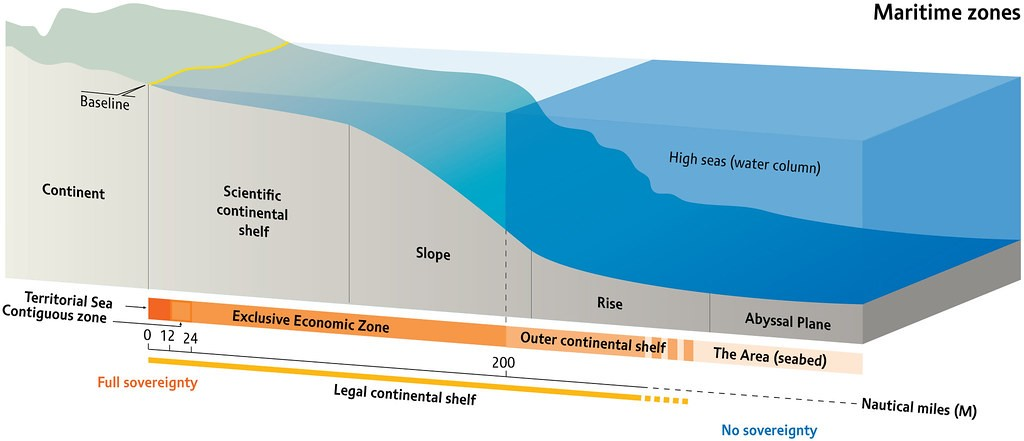
\includegraphics[width=1\textwidth]{Images/UNCLOS Maritime Zones.jpeg}
    \caption{Maritime Zones as Defined in the UNCLOS (Alternative Representation)}
    \label{fig:UNCLOS Maritime Zones}
\end{figure}

\begin{itemize}
    \item There are a number of different lines and zones that are important in international law
    \item Baselines
    \begin{itemize}
        \item Normal baselines follow the contours of the coast in all of its sinuosity, following \convention{\textit{UNCLOS} Art 5} (these are the default baselines)
        \item Straight baselines, which are used in cases primarily where the coast is deeply indented/otherwise irregular, are special baselines that are drawn up upon dots along the coast, following \convention{\textit{UNCLOS} Art 7}
        \item Coastal baselines may take a combination of normal and straight baselines, depending on the complexity and geometry of the coast
        \item Baselines are necessary as a projection point for maritime zones
    \end{itemize}
\end{itemize}

\begin{conventiondetails}{\textit{UNCLOS} Articles 5, 7}
    \flushleft
    \tcbsubtitle{Article 5}
    \textit{Normal baseline}

    \vspace{\baselineskip}

    Except where otherwise provided in this Convention, the normal baseline for measuring the breadth of the territorial sea is the low-water line along the coast as marked on large-scale charts officially recognized by the coastal State.

    \tcbsubtitle{Article 7}
    \textit{Straight baselines}
    \begin{enumerate}
        \item In localities where the coastline is deeply indented and cut into, or if there is a fringe of islands along the coast in its immediate vicinity, the method of straight baselines joining appropriate points may be employed in drawing the baseline from which the breadth of the territorial sea is measured.
        \item Where because of the presence of a delta and other natural conditions the coastline is highly unstable, the appropriate points may be selected along the furthest seaward extent of the low-water line and, notwithstanding subsequent regression of the low-water line, the straight baselines shall remain effective until changed by the coastal State in accordance with this Convention.
        \item The drawing of straight baselines must not depart to any appreciable extent from the general direction of the coast, and the sea areas lying within the lines must be sufficiently closely linked to the land domain to be subject to the regime of internal waters.
        \item Straight baselines shall not be drawn to and from low-tide elevations, unless lighthouses or similar installations which are permanently above sea level have been built on them or except in instances where the drawing of baselines to and from such elevations has received general international recognition.
        \item Where the method of straight baselines is applicable under paragraph 1, account may be taken, in determining particular baselines, of economic interests peculiar to the region concerned, the reality and the importance of which are clearly evidenced by long usage.
        \item The system of straight baselines may not be applied by a State in such a manner as to cut off the territorial sea of another State from the high seas or an exclusive economic zone.
    \end{enumerate}
\end{conventiondetails}

\subsection{Maritime Zones}
\subsubsection{Territorial Sea}
\begin{itemize}
    \item The territorial sea is an inherent, non-claimable zone
    \item It extends 12 nautical miles from the baseline, following \convention{\textit{UNCLOS} Art 3}
    \item States have territorial sovereignty in this area; they own it, and have extensive authority
    \item There are very few exceptions to this authority - the most prevalent is the right of innocent passage
\end{itemize}

\begin{conventiondetails}{\textit{UNCLOS} Articles 2-4}
    \flushleft
    \tcbsubtitle{Article 2}
    \textit{Legal status of the territorial sea, of the air space over the territorial sea and of its bed and subsoil}
    \begin{enumerate}
        \item The sovereignty of a coastal State extends, beyond its land territory and internal waters and, in the case of an archipelagic State, its archipelagic waters, to an adjacent belt of sea, described as the territorial sea.
        \item This sovereignty extends to the air space over the territorial sea as well as to its bed and subsoil.
        \item The sovereignty over the territorial sea is exercised subject to this Convention and to other rules of international law.
    \end{enumerate}

    \tcbsubtitle{Article 3}
    \textit{Breadth of the territorial sea}

    \vspace{\baselineskip}

    Every State has the right to establish the breadth of its territorial sea up to a limit not exceeding 12 nautical miles, measured from baselines determined in accordance with this Convention.

    \tcbsubtitle{Article 4}
    \textit{Outer limit of the territorial sea}

    \vspace{\baselineskip}

    The outer limit of the territorial sea is the line every point of which is at a distance from the nearest point of the baseline equal to the breadth of the territorial sea.
\end{conventiondetails}

\subsubsection{Contiguous Zone}
\begin{itemize}
    \item The contiguous zone is an enforcement zone for customs (the movement of goods), tax, immigration and quarantine laws
    \item It operates in the 12-24 nautical mile range from the baseline, right after the territorial sea, following \convention{\textit{UNCLOS} Art 33(2)}
    \item Coastal states can enforce the law against vessels only in the matters of customs, tax, immigration and quarantine
    \item The origins of this zone go back to the US Prohibition era, when people were attempting to smuggle alcohol into the US
    \item This is not a zone of sovereignty, but is rather a zone of enforcement jurisdiction
\end{itemize}

\begin{conventiondetails}{\textit{UNCLOS} Article 33}
    \flushleft
    \textit{Contiguous Zone}
    \begin{enumerate}
        \item In a zone contiguous to its territorial sea, described as the contiguous zone, the coastal State may exercise the control necessary to:
        \begin{enumerate}[label=(\alph*)]
            \item prevent infringement of its customs, fiscal, immigration or sanitary laws and regulations within its territory or territorial sea;
            \item punish infringement of the above laws and regulations committed within its territory or territorial sea.
        \end{enumerate}
        \item The contiguous zone may not extend beyond 24 nautical miles from the baselines from which the breadth of the territorial sea is measured.        
    \end{enumerate}
    
\end{conventiondetails}

\subsubsection{Exclusive Economic Zone (EEZ)}
\begin{itemize}
    \item This is a creation of \convention{\textit{UNCLOS}}
    \item Coastal states have the right to claim up to 200 nautical miles from the baseline as their exclusive economic zone (per \convention{\textit{UNCLOS} Art 57}), in which they have rights to all of the living and non-living resources (including everything in the soil, subsoil, water column, etc.), and everything on the surface (e.g., renewable energy resources)
    \item This is the most important zone economically
    \item This is not a zone of sovereignty, but is merely a zone where a state has the rights over resources and the right to regulate them
    \begin{itemize}
        \item For example, they cannot forbid foreign ships from passing through, but they can forbid foreign ships from fishing in the zone
    \end{itemize}
\end{itemize}

\begin{conventiondetails}{\textit{UNCLOS} Articles 55-58}
    \flushleft
    \tcbsubtitle{Article 55}
    \textit{Specific legal regime of the exclusive economic zone}

    \vspace{\baselineskip}

    The exclusive economic zone is an area beyond and adjacent to the territorial sea, subject to the specific legal regime established in this Part, under which the rights and jurisdiction of the coastal State and the rights and freedoms of other States are governed by the relevant provisions of this Convention.

    \tcbsubtitle{Article 56}
    \textit{Rights, jurisdiction and duties of the coastal State in the exclusive economic zone}
    \begin{enumerate}
        \item In the exclusive economic zone, the coastal State has:
        \begin{enumerate}[label=(\alph*)]
            \item sovereign rights for the purpose of exploring and exploiting, conserving and managing the natural resources, whether living or non-living, of the waters superjacent to the seabed and of the seabed and its subsoil, and with regard to other activities for the economic exploitation and exploration of the zone, such as the production of energy from the water, currents and winds;
            \item jurisdiction as provided for in the relevant provisions of this Convention with regard to:
            \begin{enumerate}[label=(\roman*)]
                \item the establishment and use of artificial islands, installations and structures;
                \item marine scientific research;
                \item the protection and preservation of the marine environment;
            \end{enumerate}
            \item other rights and duties provided for in this Convention.
        \end{enumerate}
        \item In exercising its rights and performing its duties under this Convention in the exclusive economic zone, the coastal State shall have due regard to the rights and duties of other States and shall act in a manner compatible with the provisions of this Convention.
        \item The rights set out in this article with respect to the seabed and subsoil shall be exercised in accordance with Part VI.
    \end{enumerate}

    \tcbsubtitle{Article 57}
    \textit{Breadth of the exclusive economic zone}

    \vspace{\baselineskip}

    The exclusive economic zone shall not extend beyond 200 nautical miles from the baselines from which the breadth of the territorial sea is measured.

    \tcbsubtitle{Article 58}
    \textit{Rights and duties of other States in the exclusive economic zone}
    \begin{enumerate}
        \item In the exclusive economic zone, all States, whether coastal or land-locked, enjoy, subject to the relevant provisions of this Convention, the freedoms referred to in article 87 of navigation and overflight and of the laying of submarine cables and pipelines, and other internationally lawful uses of the sea related to these freedoms, such as those associated with the operation of ships, aircraft and submarine cables and pipelines, and compatible with the other provisions of this Convention.
        \item Articles 88 to 115 and other pertinent rules of international law apply to the exclusive economic zone in so far as they are not incompatible with this Part.
        \item In exercising their rights and performing their duties under this Convention in the exclusive economic zone, States shall have due regard to the rights and duties of the coastal State and shall comply with the laws and regulations adopted by the coastal State in accordance with the provisions of this Convention and other rules of international law in so far as they are not incompatible with this Part.
    \end{enumerate}
\end{conventiondetails}

\subsubsection{Continental Shelf}
\begin{itemize}
    \item The continental shelf is an inherent seabed resources zone, and a prolongation of a state's territory
    \item States have ownership of the resources on sea bed and the subsoil, and of any living resources that live on the seabed (e.g., crustaceans, sea snails, etc.)
    \item This overlaps to a significant extent with the EEZ
\end{itemize}

\begin{conventiondetails}{\textit{UNCLOS} Articles 76-77}
    \flushleft
    \tcbsubtitle{Article 76}
    \textit{Definition of the continental shelf}

    \begin{enumerate}
        \item The continental shelf of a coastal State comprises the seabed and
        subsoil of the submarine areas that extend beyond its territorial sea
        throughout the natural prolongation of its land territory to the outer edge of
        the continental margin, or to a distance of 200 nautical miles from the
        baselines from which the breadth of the territorial sea is measured where the
        outer edge of the continental margin does not extend up to that distance.
        \item The continental shelf of a coastal State shall not extend beyond the
        limits provided for in paragraphs 4 to 6.
        \item The continental margin comprises the submerged prolongation of the
        land mass of the coastal State, and consists of the seabed and subsoil of the
        shelf, the slope and the rise. It does not include the deep ocean floor with its
        oceanic ridges or the subsoil thereof.
        \item 
        \begin{enumerate}[label=(\alph*)]
            \item For the purposes of this Convention, the coastal State shall establish the outer edge of the continental margin wherever the margin extends beyond 200 nautical miles from the baselines from which the breadth of the territorial sea is measured, by either:
            \begin{enumerate}[label=(\roman*)]
                \item a line delineated in accordance with paragraph 7 by reference to the outermost fixed points at each of which the thickness of sedimentary rocks is at least 1 per cent of the shortest distance from such point to the foot of the continental slope; or
                \item a line delineated in accordance with paragraph 7 by reference to fixed points not more than 60 nautical miles from the foot of the continental slope.
            \end{enumerate}
            \item In the absence of evidence to the contrary, the foot of the
            continental slope shall be determined as the point of maximum
            change in the gradient at its base.
        \end{enumerate}
        \item The fixed points comprising the line of the outer limits of the continental shelf on the seabed, drawn in accordance with paragraph 4 (a)(i) and (ii), either shall not exceed 350 nautical miles from the baselines from which the breadth of the territorial sea is measured or shall not exceed 100 nautical miles from the 2,500 metre isobath, which is a line connecting the depth of 2,500 metres.
        \item Notwithstanding the provisions of paragraph 5, on submarine ridges, the outer limit of the continental shelf shall not exceed 350 nautical miles from the baselines from which the breadth of the territorial sea is measured. This paragraph does not apply to submarine elevations that are natural components of continental margin, such as its plateaux, rises, caps, banks and spurs.
        \item The coastal State shall delineate the outer limits of its continental shelf, where that shelf extends beyond 200 nautical miles from the baselines from which the breadth of the territorial sea is measured, by straight lines not exceeding 60 nautical miles in length, connecting fixed points, defined by coordinates of latitude and longitude.
        \item Information on the limits of the continental shelf beyond 200 nautical miles from the baselines from which the breadth of the territorial sea is measured shall be submitted by the coastal State to the Commission on the Limits of the Continental Shelf set up under Annex II on the basis of equitable geographical representation. The Commission shall make recommendations to coastal States on matters related to the establishment of the outer limits of their continental shelf. The limits of the shelf established by a coastal State on the basis of these recommendations shall be final and binding.
        \item The coastal State shall deposit with the Secretary-General of the United Nations charts and relevant information, including geodetic data, permanently describing the outer limits of its continental shelf. The Secretary-General shall give due publicity thereto.
        \item The provisions of this article are without prejudice to the question of delimitation of the continental shelf between States with opposite or adjacent coasts.
    \end{enumerate}

    \tcbsubtitle{Article 77}
    \textit{Rights of coastal States over continental shelf}

    \begin{enumerate}
        \item The coastal State exercises over the continental shelf sovereign rights for the purpose of exploring it and exploiting its natural resources.
        \item The rights referred to in paragraph 1 are exclusive in the sense that if the coastal State does not explore the continental shelf or exploit its natural resources, no one may undertake these activities without the express consent of the coastal State.
        \item The rights of the coastal State over the continental shelf do not depend on occupation, effective or notional, or on any express proclamation.
        \item The natural resources referred to in this Part consist of the mineral and other non-living resources of the seabed and subsoil together with living organisms belonging to sedentary species, that is to say, organisms which, at the harvestable stage, either are immobile on or under the seabed or are unable to move except in constant physical contact with the seabed or the subsoil.
    \end{enumerate}
\end{conventiondetails}

\subsubsection{High Seas}
\begin{itemize}
    \item These are areas of the sea that are not subject to the jurisdiction of any state, and are open to all states
    \item They cannot be claimed by any state, and are thus non-appropriable
    \item There are certain cardinal freedoms on the high seas that cannot be violated (e.g., navigation, freedom)
\end{itemize}

\begin{conventiondetails}{\textit{UNCLOS} Articles 86-90}
    \flushleft
    \tcbsubtitle{Article 86}
    \textit{Application of the provisions of this Part}

    \vspace{\baselineskip}

    The provisions of this Part apply to all parts of the sea that are not included in the exclusive economic zone, in the territorial sea or in the internal waters of a State, or in the archipelagic waters of an archipelagic State. This article does not entail any abridgement of the freedoms enjoyed by all States in the exclusive economic zone in accordance with article 58.

    \tcbsubtitle{Article 87}
    \textit{Freedom of the high seas}
    \begin{enumerate}
        \item The high seas are open to all States, whether coastal or land-locked. Freedom of the high seas is exercised under the conditions laid down by this Convention and by other rules of international law. It comprises, inter alia, both for coastal and land-locked States:
        \begin{enumerate}[label=(\alph*)]
            \item freedom of navigation;
            \item freedom of overflight;
            \item freedom to lay submarine cables and pipelines, subject to Part VI;
            \item freedom to construct artificial islands and other installations permitted under international law, subject to Part VI;
            \item freedom of fishing, subject to the conditions laid down in section 2;
            \item freedom of scientific research, subject to Parts VI and XIII.
        \end{enumerate}
        \item These freedoms shall be exercised by all States with due regard for the interests of other States in their exercise of the freedom of the high seas, and also with due regard for the rights under this Convention with respect to activities in the Area.
    \end{enumerate}

    \tcbsubtitle{Article 88}
    \textit{Reservation of the high seas for peaceful purposes}

    \vspace{\baselineskip}

    The high seas shall be reserved for peaceful purposes.
    
    \tcbsubtitle{Article 89}
    \textit{Invalidity of claims of sovereignty over the high seas}

    \vspace{\baselineskip}

    No State may validly purport to subject any part of the high seas to its sovereignty.

    \tcbsubtitle{Article 90}
    \textit{Right of navigation}

    \vspace{\baselineskip}
    Every State, whether coastal or land-locked, shall enjoy the right to sail ships flying its fag on the high seas.
\end{conventiondetails}

\subsubsection{Archipelagic Waters}
\begin{itemize}
    \item These were created under \convention{\textit{UNCLOS} Part IV}
    \item These are the waters within an archipelago
    \item All of these waters are held to be very similar to the territorial sea
\end{itemize}

\begin{conventiondetails}{\textit{UNCLOS} Articles 46 - 49}
    \flushleft
    \tcbsubtitle{Article 46}
    \textit{Use of terms}

    \vspace{\baselineskip}

    For the purposes of this Convention:
    \begin{enumerate}[label=(\alph*)]
        \item ``archipelagic State" means a State constituted wholly by one or more archipelagos and may include other islands;
        \item ``archipelago" means a group of islands, including parts of islands, interconnecting waters and other natural features which are so closely interrelated that such islands, waters and other natural features form an intrinsic geographical, economic and political entity, or which historically have been regarded as such.
    \end{enumerate}

    \tcbsubtitle{Article 47}
    \textit{Archipelagic baselines}
    \begin{enumerate}
        \item An archipelagic State may draw straight archipelagic baselines joining the outermost points of the outermost islands and drying reefs of the archipelago provided that within such baselines are included the main islands and an area in which the ratio of the area of the water to the area of the land,including atolls, is between 1 to 1 and 9 to 1.
        \item The length of such baselines shall not exceed 100 nautical miles, except that up to 3 per cent of the total number of baselines enclosing any archipelago may exceed that length, up to a maximum length of 125 nautical miles.
        \item The drawing of such baselines shall not depart to any appreciable extent from the general configuration of the archipelago.
        \item Such baselines shall not be drawn to and from low-tide elevations, unless lighthouses or similar installations which are permanently above sea level have been built on them or where a low-tide elevation is situated wholly or partly at a distance not exceeding the breadth of the territorial sea from the nearest island.
        \item The system of such baselines shall not be applied by an archipelagic State in such a manner as to cut off from the high seas or the exclusive economic zone the territorial sea of another State.
        \item If a part of the archipelagic waters of an archipelagic State lies between two parts of an immediately adjacent neighbouring State, existing rights and all other legitimate interests which the latter State has traditionally exercised in such waters and all rights stipulated by agreement between those States shall continue and be respected.
        \item For the purpose of computing the ratio of water to land under paragraph l, land areas may include waters lying within the fringing reefs of islands and atolls, including that part of a steep-sided oceanic plateau which is enclosed or nearly enclosed by a chain of limestone islands and drying reefs lying on the perimeter of the plateau.
        \item The baselines drawn in accordance with this article shall be shown on charts of a scale or scales adequate for ascertaining their position. Alternatively, lists of geographical coordinates of points, specifying the geodetic datum, may be substituted.
        \item The archipelagic State shall give due publicity to such charts or lists of geographical coordinates and shall deposit a copy of each such chart or list with the Secretary-General of the United Nations.
    \end{enumerate}

    \tcbsubtitle{Article 48}
    \textit{Measurement of the breadth of the territorial sea, the contiguous zone,
    the exclusive economic zone and the continental shelf}

    \vspace{\baselineskip}

    The breadth of the territorial sea, the contiguous zone, the exclusive economic zone and the continental shelf shall be measured from archipelagic baselines drawn in accordance with article 47.

    \tcbsubtitle{Article 49}
    \textit{Legal status of archipelagic waters, of the air space over archipelagic waters and of their bed and subsoil}
    \begin{enumerate}
        \item The sovereignty of an archipelagic State extends to the waters enclosed by the archipelagic baselines drawn in accordance with article 47, described as archipelagic waters, regardless of their depth or distance from the coast.
        \item This sovereignty extends to the air space over the archipelagic waters, as well as to their bed and subsoil, and the resources contained therein.
        \item This sovereignty is exercised subject to this Part.
        \item The regime of archipelagic sea lanes passage established in this Part shall not in other respects affect the status of the archipelagic waters, including the sea lanes, or the exercise by the archipelagic State of its sovereignty over such waters and their air space, bed and subsoil, and the resources contained therein.
    \end{enumerate}

\end{conventiondetails}

\subsubsection{Deep Seabed}
\begin{itemize}
    \item This is referred to as `the Area' in the \convention{\textit{UNCLOS}}, and is considered as the common heritage of mankind
    \item Once an individual/ship leaves the continental shelf and enters the deep seabed, it cannot be appropriated by any state; it is instead vested in all people (i.e., they have a stake in it)
    \item The International Seabed Authority (established by \convention{\textit{UNCLOS}} and based in Jamaica) is responsible for the management of the deep seabed by issuing licences on an equitable basis to ensure all countries can access the resources in the deep sea
    \item The deep sea lies immediately below the high seas
\end{itemize}

\begin{casedetails}{\textit{South China Sea Arbitration (Philippines v China)} [2016] PCA}
    \flushleft
    Prior to 2016, the Philippines challenged China's claim to the entirety of the South China Sea, and to China's assertion of maritime zones from particular features in the Sea. The Tribunal examining these issues was established under \convention{\textit{UNCLOS}}.

    \vspace{\baselineskip}

    The first key issue was China's `Nine-Dash Line', which was held to be incompatible with \convention{\textit{UNCLOS}}. This is because the zone extended very substantially beyond China's coastline, and well beyond the 200 nautical mile limit of the EEZ. The Tribunal held that the Nine-Dash Line was not a valid claim to maritime zones, and that China had no rights to the waters within the line. Moreover, as China was a party to \convention{\textit{UNCLOS}}, any historical claims were extinguished upon the signing of the treaty, and so historical maritime zones could not be argued.

    \vspace{\baselineskip}

    Moreover, none of the maritime features in dispute were islands as defined in \convention{\textit{UNCLOS}}. The Tribunal held that none of the features were capable of generating an EEZ or continental shelf, and that they were all either rocks or low-tide elevations. As such, the Tribunal held that China had no rights to any maritime zones from these features. At most, they could generate a territorial sea, but not an EEZ or continental shelf. The Tribunal also held that China had violated the Philippines' rights in the EEZ, and that China had failed to protect the marine environment in the area.
\end{casedetails}

\section{Antarctica}
\begin{itemize}
    \item There are 7 claimants to territory in Antarctica: Argentina, Australia, Chile, France, New Zealand, Norway, and the UK
    \item Article 4 of the \convention{\textit{1959 Antarctic Treaty}} provides that no new claims to territory in Antarctica may be made, but that there is no renunciation of any existing claims (i.e., they are frozen whilst the treaty is in force)
    \item Whilst the treaty is in force, no acts conducted can constitute a basis for asserting, supporting or denying a claim to territorial sovereignty in Antarctica
\end{itemize}

\begin{conventiondetails}{\textit{1959 Antarctic Treaty} Art 4}
    \flushleft 
    \begin{enumerate}
        \item Nothing contained in the present Treaty shall be interpreted as:
        \begin{enumerate}[label=(\alph*)]
            \item a renunciation by any Contracting Party of previously asserted rights of or claims to territorial sovereignty in Antarctica;
            \item a renunciation or diminution by any Contracting Party of any basis of claim to territorial sovereignty in Antarctica which it may have whether as a result of its activities or those of its nationals in Antarctica, or otherwise;
            \item prejudicing the position of any Contracting Party as regards its recognition or non-recognition of any other State's right of or claim or basis of claim to territorial sovereignty in Antarctica.
        \end{enumerate}
        \item No acts or activities taking place while the present Treaty is in force shall 
        constitute a basis for asserting, supporting or denying a claim to territorial 
        sovereignty in Antarctica or create any rights of sovereignty in Antarctica. No new 
        claim, or enlargement of an existing claim, to territorial sovereignty in Antarctica 
        shall be asserted while the present Treaty is in force.
    \end{enumerate}
\end{conventiondetails}

\section{Airspace and Outer Space}

\subsection{Airspace}
\begin{itemize}
    \item A state has sovereignty over the airspace above its territory and territorial sea (\textit{cujus est solum ejus est usque ad coelum})
    \item Other states have the freedom of overflight over the contiguous zone, the EEZ, and high seas
    \item The boundary between national airspace and outer space is not clearly defined
\end{itemize}

\subsection{Outer Space}
\begin{itemize}
    \item The \convention{\textit{1967 Outer Space Treaty} Art 2} provides that outer space is not subject to national appropriation by any means
    \item Article 1 of this treaty additionally holds that outer space is the province of mankind
    \item There are 113 parties to this treaty
\end{itemize}

\begin{conventiondetails}{\textit{1967 Outer Space Treaty}}
    \flushleft
    \tcbsubtitle{Article 1}
    The exploration and use of outer space, including the moon and other celestial bodies, shall be carried out for the benefit and in the interests of all countries, irrespective of their degree of economic or scientific development, and shall be the province of all mankind.

    \vspace{\baselineskip}
    
    Outer space, including the moon and other celestial bodies, shall be free for exploration and use by all States without discrimination of any kind, on a basis of equality and in accordance with international law, and there shall be free access to all areas of celestial bodies.

    \vspace{\baselineskip}
    
    There shall be freedom of scientific investigation in outer space, including the moon and other celestial bodies, and States shall facilitate and encourage international co-operation in such investigation.
    \tcbsubtitle{Article 2}
    Outer space, including the moon and other celestial bodies, is not subject to national appropriation by claim of sovereignty, by means of use or occupation, or by any other means.
\end{conventiondetails}

\begin{itemize}
    \item The \convention{\textit{1979 Moon Agreement} Art 11(1)} provides that the moon and other celestial bodies are the common heritage of mankind
    \item There are only 18 parties to this treaty
\end{itemize}

\begin{conventiondetails}{\textit{1979 Agreement Governing the Activities of States on the Moon and Other Celestial Bodies}}
    \flushleft
    \tcbsubtitle{Article 11}
    \begin{enumerate}
        \item The moon and its natural resources are the common heritage of mankind, which finds its expression in the provisions of this Agreement, in particular in paragraph 5 of this article.
        \item The moon is not subject to national appropriation by any claim of sovereignty, by means of use or occupation, or by any other means.
        \item Neither the surface nor the subsurface of the moon, nor any part thereof or natural resources in place, shall become property of any State, international intergovernmental or non- governmental organization, national organization or non-governmental entity or of any natural person. The placement of personnel, space vehicles, equipment, facilities, stations and installations on or below the surface of the moon, including structures connected with its surface or subsurface, shall not create a right of ownership over the surface or the subsurface of the moon or any areas thereof. The foregoing provisions are without prejudice to the international regime referred to in paragraph 5 of this article.
        \item States Parties have the right to exploration and use of the moon without discrimination of any kind, on the basis of equality and in accordance with international law and the terms of this Agreement.
        \item States Parties to this Agreement hereby undertake to establish an international regime, including appropriate procedures, to govern the exploitation of the natural resources of the moon as such exploitation is about to become feasible. This provision shall be implemented in accordance with article 18 of this Agreement.
        \item In order to facilitate the establishment of the international regime referred to in paragraph 5 of this article, States Parties shall inform the Secretary-General of the United Nations as well as the public and the international scientific community, to the greatest extent feasible and practicable, of any natural resources they may discover on the moon.
        \item The main purposes of the international regime to be established shall include:
        \begin{enumerate}[label=(\alph*)]
            \item The orderly and safe development of the natural resources of the moon;
            \item The rational management of those resources;
            \item The expansion of opportunities in the use of those resources;
            \item An equitable sharing by all States Parties in the benefits derived from those resources, whereby the interests and needs of the developing countries, as well as the efforts of those countries which have contributed either directly or indirectly to the exploration of the moon, shall be given special consideration.
        \end{enumerate}
        \item All the activities with respect to the natural resources of the moon shall be carried out in a manner compatible with the purposes specified in paragraph 7 of this article and the provisions of article 6, paragraph 2, of this Agreement.
    \end{enumerate}
\end{conventiondetails}

\chapter{Jurisdiction}
\begin{itemize}
    \item State jurisdiction refers to the power or competence of a state to prescribe or enforce its laws
    \item State jurisdiction includes:
    \begin{itemize}
        \item \textbf{Prescriptive jurisdiction}, which is the power to enact laws/assert jurisdiction by legislation (legislative power)
        \item \textbf{Adjudicative jurisdiction}, which is the power to apply laws and decide disputes (judicial power)
        \item \textbf{Enforcement jurisdiction}, which is the ability to enforce laws within a state's territory (executive power)
    \end{itemize}
    \item Enforcement jurisdiction is almost always confined to a state's territory, but prescriptive jurisdiction is becoming increasingly extraterritorial
    \item The litmus test for the limits of state jurisdiction is \textbf{protest by other states}
    \item The rules around custom in relation to jurisdiction have been formed by states asserting jurisdiction, and by some states resisting/opposing jurisdiction
\end{itemize}

\section{Civil Jurisdiction}
\begin{itemize}
    \item Civil jurisdiction refers to the exercise by states of power (prescriptive and adjudicative) over persons, matters or things in private disputes (e.g., torts, contracts, family law, etc.)
    \item International law places very few limits on the assertion of civil jurisdiction, taking a hands-off approach to the power of states
    \item This has resulted in many situations where states have been extravagant in exercising civil powers internationally
    \item For example, the \statute{\textit{Alien Tort Claims Act 1789} (US)} conferred jurisdiction on US federal courts in civil actions by non-nationals for violations of international law
    \begin{itemize}
        \item Following a revitalisation of this law in the 1980s, it has now been interpreted restrictively by the US Supreme Court (see \case{\textit{Sosa v Alvare-Machain} (SCOTUS, 2004)} and \case{\textit{Kiobel v Royal Dutch Petroleum} (SCOTUS, 2013)})
        \item In \case{\textit{Kiobel v Royal Dutch Petroleum}}, Nigerian plaintiffs were injured by Royal Dutch Petroleum
        \item In \case{\textit{Sosa v Alvare-Machain}}, a Mexican national was kidnapped by US agents in Mexico and brought to the US for trial
    \end{itemize}
\end{itemize}

\section{Criminal Jurisdiction}

\subsection{Territorial Principle}

\subsection{Nationality Principle}

\subsection{Protective Principle}

\subsection{Passive Personality Principle}

\subsection{Universality Principle}

\section{Jurisdiction of the ICJ}

\subsection{Relevance of Illegally Obtained Custody}

\chapter{Immunity from Jurisdiction I}
\begin{itemize}
    \item Whilst states enjoy complete and exclusive jurisdiction within their own territories, foreign states (including foreign state officials and diplomatic representatives) enjoy a range of immunities from the jurisdiction in the forum
    \item The foreign state and diplomatic immunities operate as a procedural bar to the exercise of jurisdiction (i.e., there is still jurisdiction, but it cannot be imposed)
    \begin{itemize}
        \item This immunity can be waived by the foreign agent or their state
    \end{itemize}
    \item Foreign state immunity is less extensive than it once was, with the predominant mode of operation having shifted to `restrictive immunity', where states can be sued in relation to commercial transactions (although diplomatic immunity remains largely unchanged over the years)
\end{itemize}

\section{Foreign State Immunity}
\begin{itemize}
    \item The principle of foreign state immunity is that one sovereign state (the forum state) may not adjudicate on the conduct of a foreign state (e.g., in an Australian court, foreign states would have immunity from proceedings)
    \begin{itemize}
        \item It is no longer the case that foreign states enjoy complete immunity; there are now a variety of circumstances in which a foreign state may be subject to the jurisdiction of a court that is not protected by an immunity
    \end{itemize}
    \item Subject to certain exceptions, the foreign state and its officials enjoy procedural immunity from criminal and civil proceedings in the forum state (i.e., foreign states, their officials and representatives (e.g., head of state, head of government, ministers, etc.) can enjoy immunity from proceedings within the forum), following Lord Brown-Wilkinson in \case{\textit{Pinochet (No 3)} [1999] 2 All ER 97} (see Page \pageref{case:Pinochet (No 3)})
    \item This is derived from the idea that all sovereign states are equal, and that one state does not have power over another (\textit{par in partem non habet imperium})
    \begin{itemize}
        \item This has been held to be ``one of the fundamental principles of the international legal order'' in \case{\textit{Jurisdictional Immunities Case} [2012] ICJ Rep 99}
    \end{itemize}
    \item There are two approaches/theories to foreign state immunity: `absolute immunity' and `restrictive immunity'
\end{itemize}

\subsection{Absolute Immunity Principle}
\begin{itemize}
    \item The absolute immunity principle holds that state are completely immune from the jurisdiction of another state; i.e., they are immune from any and all proceedings in the forum state
    \item Whilst this has now been eroded, it was the classical position
    \begin{itemize}
        \item ```[T]he perfect equality and absolute independence of sovereigns' mean no state can be made subject to the jurisdiction of another against its will'' - \case{\textit{The Schooner Exchange v McFaddon} (US Supreme Court, 1812)}
        \item In the modern day, only a few developing states tend to adhere to this absolute view of state immunity
    \end{itemize}  
\end{itemize}

\begin{casedetails}{\textit{The Schooner Exchange v McFaddon} (US Supreme Court, 1812)}
    \flushleft
    In a notable maritime case, a private vessel that sailed from Baltimore to Spain was seized by Napoleon en route and pressed into service for the French navy. The vessel later docked in Philadelphia, where its original American owners sought to reclaim it. The U.S. Supreme Court, in addressing the case, articulated the principle of absolute immunity for foreign naval vessels. The Court ruled that, regardless of the original ownership, the vessel was now a French naval ship and thus entitled to immunity, depriving the plaintiffs of jurisdiction to pursue their claim. This principle of sovereign immunity for naval vessels remains applicable today, shielding such ships from legal actions in foreign courts.
\end{casedetails}

\begin{itemize}
    \item In recent years, China abandoned this principle in favour of the restrictive immunity principle by adopting the \statute{\textit{Foreign States Immunity Law 2024}}, which largely follows the \convention{\textit{UN Convention on Jurisdictional Immunities of States and Their Property}} (this is noteworthy as the Convention has not yet entered into force, but is still influential as a statement of general principle)
    \begin{itemize}
        \item Prior to this, China's adherence to the absolute immunity principle was evident in \case{\textit{DRC v F C Hemisphere} [2011] HKFCA 43}, which applied absolute immunity in commercial proceedings against the government of the Democratic Republic of Congo
    \end{itemize}
\end{itemize}

\subsection{Restrictive Immunity Principle}
\begin{itemize}
    \item The restrictive immunity principle holds that foreign states are afforded immunity only with respect to acts of a sovereign or governmental character (\textit{acta jure imperii}), not for acts of a commercial character (\textit{acta jure gestionis}) (or any other non-sovereign acts); this is the prevailing approach across the world
    \item The restrictive immunity principle has been deemed necessary in the interests of justice to allow individuals to bring commercial transactions before the courts, thereby resolving the unfairness in commercial disputes between states and individuals as it does not impede the sovereignty of the foreign state
    \item This principle has been rationalised on the basis of not infringing on state sovereignty, as it only affects acts which have a commercial aspect to them and does not prevent states from undertaking sovereign acts
\end{itemize}

\begin{casedetails}{\textit{I Congresso del Partido} (1983) HoL}
    \flushleft
    A dispute arose when ships owned by the Cuban government failed to deliver a sugar cargo to Chile, prompting the cargo owners to initiate legal action against the ships and the Cuban government in the United Kingdom. The case stemmed from a contract between a Cuban state trading company and a Chilean company for the sale and delivery of sugar. Following a coup in Chile that brought Augusto Pinochet to power, Cuba directed its vessels to withhold the cargo, leading to proceedings in the UK courts. The Cuban government claimed sovereign immunity to shield itself from the lawsuit. However, the House of Lords, led by Lord Wilberforce and with the agreement of the other Law Lords, rejected this claim. The court applied a restrictive immunity approach, focusing on the nature of the act rather than its purpose. Despite the political motivation behind Cuba's decision to halt the sugar delivery, the transaction was deemed a commercial one, rooted in a trading relationship. Consequently, the court held that Cuba was not entitled to immunity, allowing the legal action to proceed against the Cuban vessel, and upholding the restrictive immunity principle.
\end{casedetails}

\begin{itemize}
    \item The majority of states have adopted the restrictive immunity principle
    \item This approach was moreover adopted in the \convention{\textit{2004 Convention on Jurisdictional Immunities of States and Their Property}}
    \begin{itemize}
        \item This Convention had, as of 14/04/2025, 24 parties, falling short of the 30 required for it to enter into force
        \item As such, it acts as a partial codification of customary international law, especially in relation to the provisions around restrictive immunity
    \end{itemize}
    \item In Australia, the relevant legislation is the \statute{\textit{Foreign States Immunities Act 1985 (Cth)}}, which was enacted following an ALRC inquiry on Foreign State Immunity in 1984
    \begin{itemize}
        \item The ALRC stated that ``In the interests of avoiding possible foreign relations problems, Australia should articulate to foreign states more precise rules governing their liability to the jurisdiction of the Australian courts."
        \item This Act adopts the restrictive immunity principle in Australia
    \end{itemize}
\end{itemize}

\section{Foreign States Immunities Act 1985 (Cth)}

\subsection{Section 9}
\begin{statutedetails}{\textit{Foreign States Immunities Act 1985 (Cth)} Section 9}
    \flushleft
    \textbf{General immunity from jurisdiction}

    \vspace{\baselineskip}

    Except as provided by or under this Act, a foreign State is immune from the jurisdiction of the courts of Australia in a proceeding.
\end{statutedetails}

\begin{itemize}
    \item Under \statute{s 3(1)}, a proceeding means a civil proceeding, not a prosecution for an offence (i.e., not a criminal proceeding)
    \item It was held in \case{\textit{PT Garuda v ACCC} [2012] HCA 33} that a proceeding includes a proceeding commenced by the ACCC against a defendant seeking penalties for anti-competitive conduct
\end{itemize}

\begin{casedetails}{\textit{Pt Garuda v ACCC} [2012] HCA 33}
    \flushleft
    Garuda was an Indonesia state-owned airline. The ACCC brought proceedings against them, alleging that Garuda had entered into anti-competitive conduct in relation to air-freight services into Australia. The Court held that a proceeding under \statute{\textit{Foreign States Immunities Act 1985 (Cth)} s 3} did extend to include not just proceedings in matters such as tort, but also proceedings brought by a regulator (including the ACCC0 seeking civil penalties for breaches of the Australian consumer law). From this case, it is established that there is a general immunity of foreign states from the jurisdiction of a state, subject to certain identified immunities.
\end{casedetails}

\begin{itemize}
    \item \statute{\textit{Foreign States Immunities Act 1985 (Cth)} ss 10-21} establish exceptions to the general immunity afforded under \statute{s 9}
    \item The general immunity afforded under \statute{s 9} applies to foreign states (including organs of foreign states), and also `separate entities' of foreign states (agencies/instrumentalities of state)
    \begin{itemize}
        \item This applies to all parts of a foreign state's government and organs of that government
        \item This serves to capture the case where states have established statutory organisations to carry out activities usually done by the government
    \end{itemize}
    \item The classic example of this is foreign airlines, such as in the case of \case{\textit{PT Garuda v ACCC} [2011] FCFCA 52} (this is the Federal Court, not the High Court version on Page \pageref{case:ACCC v Garuda})
    \begin{itemize}
        \item The key question in the case was whether Garuda was to be considered a separate entity of Indonesia?
        \begin{itemize}
            \item If it was, it was entitled to immunity unless there was an exception enlivened
        \end{itemize}
        \item Lander and Greenwood JJ held that ``[t]he most relevant factor in determining whether a natural person or a corporation is an agency or instrumentality is whether that body is carrying out the foreign State's functions or purposes ... regard will be had to ownership, control, the functions which the natural person or corporation perform, the foreign State's purposes in supporting the [alleged separate entity] and the manner in which the [separate entity] conducts itself or its business.''
        \begin{itemize}
            \item It is imperative to look at the ownership of the entity and the functions that are being executed, as well as the overriding functional purpose
            \item A company with some association with the State may fall under this, depending on how close it is to the state
        \end{itemize}
    \end{itemize}
    \item Under \statute{ss 30-32}, unless there has been a waiver, only the commercial property of a state may be the subject of execution of a judgement (commercial property is property in use by the foreign state substantially for commercial purposes, and does not include diplomatic or military property)
    \begin{itemize}
        \item Judgement cannot be enforced against sovereign property
    \end{itemize}
\end{itemize}

\begin{casedetails}{\textit{Firebird Global Master Fund II Ltd v Nauru} (2015) 326 ALR 396}
    \flushleft
    Firebird sought to register and enforce in Australia a Japanese judgment obtained against Nauru, related to bearer bonds guaranteed by Nauru. The High Court of Australia determined that the commercial transaction exception applied, as the Japanese judgment pertained to a commercial transaction. However, Nauru's bank accounts in Australia were deemed immune from any legal process or order, as they were used exclusively for governmental purposes rather than commercial activities. Consequently, the cash held in these accounts could not be subjected to a garnishing order or used to enforce the judgment.

    \flushleft

    Although Firebird successfully had the foreign judgment recognised in Australia and overcame the initial hurdle of \statute{\textit{Foreign States Immunities Act 1985 (Cth)} Section 9}, which governs immunity from jurisdiction, the enforcement effort ultimately failed due to the absence of available assets. The immunity of Nauru's bank accounts, reserved for governmental functions, presented an insurmountable barrier, leaving Firebird unable to execute the judgment. This case highlights the challenges of enforcing foreign judgments against sovereign states when their assets are protected for non-commercial purposes.

\end{casedetails}

\subsection{Section 10}
\begin{statutedetails}{\textit{Foreign States Immunities Act 1985 (Cth)} Section 10}
    \flushleft
    \textbf{Submission to jurisdiction}

    \begin{enumerate}[label=(\arabic*)]
        \item A foreign State is not immune in a proceeding in which it has submitted to the jurisdiction in accordance with this section.
        \item A foreign State may submit to the jurisdiction at any time, whether by agreement or otherwise, but a foreign State shall not be taken to have so submitted by reason only that it is a party to an agreement the proper law of which is the law of Australia.
        \item A submission under subsection (2) may be subject to a specified limitation, condition or exclusion (whether in respect of remedies or otherwise).
        \item Without limiting any other power of a court to dismiss, stay or otherwise decline to hear and determine a proceeding, the court may dismiss, stay or otherwise decline to hear and determine a proceeding if it is satisfied that, by reason of the nature of a limitation, condition or exclusion to which a submission is subject (not being a limitation, condition or exclusion in respect of remedies), it is appropriate to do so.
        \item An agreement by a foreign State to waive its immunity under this Part has effect to waive that immunity and the waiver may not be withdrawn except in accordance with the terms of the agreement.
        \item Subject to subsections (7), (8) and (9), a foreign State may submit to the jurisdiction in a proceeding by:
        \begin{enumerate}[label=(\alph*)]
            \item instituting the proceeding; or
            \item intervening in, or taking a step as a party to, the proceeding.           
        \end{enumerate}
        \item A foreign State shall not be taken to have submitted to the jurisdiction in a proceeding by reason only that:
        \begin{enumerate}[label=(\alph*)]
            \item it has made an application for costs; or
            \item it has intervened, or has taken a step, in the proceeding for the purpose or in the course of asserting immunity.
        \end{enumerate}
        \item Where the foreign State is not a party to a proceeding, it shall not be taken to have submitted to the jurisdiction by reason only that it has intervened in the proceeding for the purpose or in the course of asserting an interest in property involved in or affected by the proceeding.
        \item Where:
        \begin{enumerate}[label=(\alph*)]
            \item the intervention or step was taken by a person who did not know and could not reasonably have been expected to know of the immunity; and
            \item the immunity is asserted without unreasonable delay;
        \end{enumerate}
        the foreign State shall not be taken to have submitted to the jurisdiction in the proceeding by reason only of that intervention or step.
        \item Where a foreign State has submitted to the jurisdiction in a proceeding, then, subject to the operation of subsection (3), it is not immune in relation to a claim made in the proceeding by some other party against it (whether by way of set - off, counter - claim or otherwise), being a claim that arises out of and relates to the transactions or events to which the proceeding relates.
        \item In addition to any other person who has authority to submit, on behalf of a foreign State, to the jurisdiction:
        \begin{enumerate}[label=(\alph*)]
            \item the person for the time being performing the functions of the head of the State's diplomatic mission in Australia has that authority; and
            \item a person who has entered into a contract on behalf of and with the authority of the State has authority to submit in that contract, on behalf of the State, to the jurisdiction in respect of a proceeding arising out of the contract.
        \end{enumerate}
    \end{enumerate}
\end{statutedetails}

\begin{itemize}
    \item \statute{s 10} provides an exception to immunity where the foreign state has expressly submitted to the jurisdiction of the forum state (i.e., they've waived their immunity at their will)
    \item At times, foreign states will appeal in proceedings, but will be appearing only to contest jurisdiction; at times, they may just submit to the jurisdiction of the court
\end{itemize}

\begin{casedetails}{\textit{Kingdom of Spain v Infrastructure Services Luxembourg S.à.r.l.} [2023] HCA 11}
    \flushleft
    A company was awarded €101 million against Spain in an arbitration under the \convention{\textit{ICSID Convention}} and sought to enforce this award in Australia under the \statute{\textit{International Arbitration Act 1974 (Cth)}}. The \convention{\textit{ICSID Convention}} allows enforcement of arbitral awards in any member state's jurisdiction, including Australia. Spain invoked immunity under the Foreign States Immunities Act 1985 (Cth) to block the enforcement. The High Court of Australia (HCA) considered Article 54 of the \convention{\textit{ICSID Convention}}, which requires member states to recognize ICSID awards as binding and enforce them as if they were final domestic court judgments. The HCA interpreted section 10(2) of the Foreign States Immunities Act in accordance with international law, which mandates that any waiver of immunity must be express.
    
    \vspace{\baselineskip}
    
    The court held that such a waiver must be explicitly derived from the terms of international agreements, either as an express provision or as a term implied by necessity, as noted in paragraph [25] of the judgment. The HCA determined that Spain's agreement to Articles 53, 54, and 55 of the \convention{\textit{ICSID Convention}} constituted an express waiver of immunity from Australian court jurisdiction for the recognition and enforcement of the award, but not for its execution against Spanish sovereign property. As a result, the company could proceed with recognition and enforcement proceedings, but Spain's immunity from execution rendered the victory pyrrhic, as the award could not be executed against Spanish assets.
\end{casedetails}

\begin{casedetails}{\textit{Republic of India v CCDM Holdings, LLC} [2025] FCAFC 2}
    \flushleft
    A US\$111 million arbitral award was issued in favour of Mauritian investors in an Indian company under the India-Mauritius Bilateral Investment Treaty (BIT). The investors sought to enforce this award in Australia, relying on the 1958 New York Convention on the Recognition and Enforcement of Arbitration Awards, to which both Australia and India are parties. India had made a reservation to the Convention, limiting its application to disputes arising from legal relationships, contractual or otherwise, deemed commercial under Indian law. The investors initiated proceedings in Australia against India to enforce the award.
    
    \vspace{\baselineskip}
    
    The Federal Court of Australia (FCA) overturned the decision of Jackman J, ruling that India's reservation applied reciprocally, affecting the obligations of both Australia and India. The FCA held that Australia was not obligated to enforce awards related to disputes not considered commercial under Indian law. The court found that the award did not stem from a commercial legal relationship, as the BIT created a relationship under public international law, and the underlying dispute arose from the cancellation of a contract on public interest grounds.
    
    \vspace{\baselineskip}
    
    Furthermore, the FCA determined that India's ratification of the New York Convention did not constitute a waiver of foreign state immunity under the ``unmistakable" test established in \case{\textit{Kingdom of Spain v Infrastructure Services Luxembourg S.à.r.l.} [2023] HCA 11}, which requires a clear and explicit waiver of immunity. Consequently, the enforcement proceedings against India could not proceed in Australia.
\end{casedetails}

\begin{itemize}
    \item This Act comprehensively examines immunity issues, and there are no implied exceptions to immunity, as seen in the following cases:
    \begin{itemize}
        \item \case{\textit{Zhang v Zemin} [2010] NSWCA 255}, which was a damages proceeding against Chinese officials regarding torture
        \begin{itemize}
            \item This case held that there was no implied exception to foreign state immunity based on the \textit{jus cogens} prohibition of torture
            \item Spiegelman J stated that there was no additional justification for exceptions, even in such a grave case
        \end{itemize}
        item \case{\textit{Young v A-G (NZ) and Ministry of Defence (UK)} [2019] NZSC 23}, which was a claim in tort in respect of sexual assault during a posting of the Royal Navy in the UK
        \begin{itemize}
            \item In this case, there was no exception to immunity arising from the duty of a state to provide the human right of a right to an effective remedy
            \item The plaintiff claimed to be the victim of assault whilst in the UK, working for the Royal Navy
        \end{itemize}
    \end{itemize}
\end{itemize}

\subsection{Section 11}
\begin{statutedetails}{\textit{Foreign States Immunities Act 1985 (Cth)} Section 11}
    \flushleft
    \textbf{Commercial Transactions}

    \begin{enumerate}[label=(\arabic*)]
        \item A foreign State is not immune in a proceeding in so far as the proceeding concerns a commercial transaction.
        \item Subsection (1) does not apply:
        \begin{enumerate}
            \item if all the parties to the proceeding:
            \begin{enumerate}[label=(\roman*)]
                \item are foreign States or are the Commonwealth and one or more foreign States; or
                \item have otherwise agreed in writing; or
            \end{enumerate}
            \item in so far as the proceeding concerns a payment in respect of a grant, a scholarship, a pension or a payment of a like kind.
        \end{enumerate}
        \item In this section, \textit{\textbf{commercial transaction}} means a commercial, trading, business, professional or industrial or like transaction into which the foreign State has entered or a like activity in which the State has engaged and, without limiting the generality of the foregoing, includes:
        \begin{enumerate}[label=(\alph*)]
            \item a contract for the supply of goods or services;
            \item an agreement for a loan or some other transaction for or in respect of the provision of finance; and
            \item a guarantee or indemnity in respect of a financial obligation; but does not include a contract of employment or a bill of exchange.
        \end{enumerate} 
    \end{enumerate}
\end{statutedetails}

\begin{itemize}
    \item This section states that a foreign sate is not immune in a proceeding which concerns a commercial transaction, clearly expressing the restrictive immunity principle
    \item This is the most important section of the Act, and is invoked the most frequently
    \item `The definition of ``commercial transaction" fixes upon entry and engagement by the foreign State. It does not have any limiting terms which would restrict the immunity…to a proceeding instituted against the foreign State by a party to the commercial transaction in question ... \textbf{The arrangements and understandings into which the ACCC alleges Garuda entered were \underline{dealings of a commercial, trading and business character}}, respecting the conduct of airline freight services to Australia.', following \case{\textit{PT Garuda v ACCC} [2012] HCA 33 per French CJ, Gummow, Hayne and Crennan JJ}
    \begin{itemize}
        \item In this case, it was held that for proceedings to continue, there needed to be established some exception to immunity
        \item In this case, the Court held that the commercial transaction exception applies, as the whole character of the proceedings at hand related to commercial dealings, even though the commercial dealings were not between the ACCC and Garuda
        \item Thus, it is irrelevant if the parties were directly engaged in a commercial relationship; the exception applies if the underlying character of the case is commercial in nature
    \end{itemize}
\end{itemize}

\begin{casedetails}{\textit{Australian International Islamic College Board Inc v Saudi Arabia} [2013] QCA 129}
    \flushleft
    The government of Saudi Arabia promised to cover the costs of educating students at a college in Australia, a commitment that constituted a commercial transaction for the recipients of these scholarships. However, the Saudi government failed to fulfill this financial obligation. When legal proceedings were initiated in Queensland, Saudi Arabia invoked sovereign immunity to avoid liability. In the resulting case, Holmes JA delivered the leading judgment, with the other justices in agreement, characterising the relationship as one centred on the payment for educational services. The court determined that this was indeed a commercial transaction, and thus, section 11 of the relevant legislation applied, rendering the immunity claim inapplicable.

    \vspace{\baselineskip}

    Holmes JA further elaborated on the rationale behind the commercial transactions exception, providing clarity on its purpose and justification. As stated in the judgment: ``The relevant exception…appears to have two main foundations: (a) It is necessary in the interest of justice to individuals having such transactions with states to allow them to bring such transactions before the courts. (b) To require a state to answer a claim based upon such transactions does not involve a challenge to or inquiry into any act of sovereignty or governmental act of that state. It is ... neither a threat to the dignity of that state, nor any interference with its sovereign functions." (Holmes JA at [24]). This reasoning underscores the balance between ensuring justice for individuals and respecting state sovereignty, emphasising that commercial dealings do not infringe upon a state's governmental authority or dignity.
\end{casedetails}

\subsection{Section 12}
\begin{statutedetails}{\textit{Foreign States Immunities Act 1985 (Cth)} Section 12}
    \flushleft
    \textbf{Contracts of employment}

    \begin{enumerate}[label=(\arabic*)]
        \item A foreign State, as employer, is not immune in a proceeding in so far as the proceeding concerns the employment of a person under a contract of employment that was made in Australia or was to be performed wholly or partly in Australia.
        \item A reference in subsection (1) to a proceeding includes a reference to a proceeding concerning
        \begin{enumerate}[label=(\alph*)]
            \item a right or obligation conferred or imposed by a law of Australia on a person as employer or employee; or
            \item a payment the entitlement to which arises under a contract of employment.
        \end{enumerate}
        \item Where, at the time when the contract of employment was made, the person employed was:
        \begin{enumerate}[label=(\alph*)]
            \item a national of the foreign State but not a permanent resident of Australia ; or
            \item an habitual resident of the foreign State;
        \end{enumerate}
        subsection (1) does not apply.
        \item Subsection (1) does not apply where:
        \begin{enumerate}[label=(\alph*)]
            \item an inconsistent provision is included in the contract of employment; and
            \item a law of Australia does not avoid the operation of, or prohibit or render unlawful the inclusion of, the provision.
        \end{enumerate}
        \item Subsection (1) does not apply in relation to the employment of:
        \begin{enumerate}
            \item a member of the diplomatic staff of a mission as defined by the Vienna Convention on Diplomatic Relations, being the Convention the English text of which is set out in the Schedule to the Diplomatic Privileges and Immunities Act 1967 ; or
            \item a consular officer as defined by the Vienna Convention on Consular Relations, being the Convention the English text of which is set out in the Schedule to the Consular Privileges and Immunities Act 1972 .
        \end{enumerate}
        \item Subsection (1) does not apply in relation to the employment of:
        \begin{enumerate}[label=(\alph*)]
            \item a member of the administrative and technical staff of a mission as defined by the Convention referred to in paragraph (5)(a); or
            \item a consular employee as defined by the Convention referred to in paragraph (5)(b);
        \end{enumerate}
        unless the member or employee was, at the time when the contract of employment was made, a permanent resident of Australia.
        \item In this section, permanent resident of Australia means:
        \begin{enumerate}
            \item an Australian citizen; or
            \item a person resident in Australia whose continued presence in Australia is not subject to a limitation as to time imposed by or under a law of Australia.
        \end{enumerate}
    \end{enumerate}
\end{statutedetails}

\begin{itemize}
    \item This section states that a foreign state is not immune in a proceeding which concerns the employment of a person under a contract of employment made in Australia or performed in Australia (i.e., if you are a foreign state and employ Australians, you cannot claim immunity in this area)
\end{itemize}

\subsection{Section 13}
\begin{statutedetails}{\textit{Foreign States Immunities Act 1985 (Cth)} Section 13}
    \flushleft
    \textbf{Personal injury and damage to property}

    \vspace{\baselineskip}

    A foreign State is not immune in a proceeding in so far as the proceeding concerns:
    \begin{enumerate}[label=(\alph*)]
        \item the death of, or personal injury to, a person; or
        \item loss of or damage to tangible property;
    \end{enumerate}
    caused by an act or omission done or omitted to be done in Australia.
\end{statutedetails}

\begin{itemize}
    \item This section states that a foreign state is not immune in a proceeding concerning death, personal injury, or loss or damage of tangible property, caused by an act or omission \underline{in Australia} (the `local torts' exception)
\end{itemize}

\begin{casedetails}{\textit{Tokic v Government of Yugoslavia} (1999) NSWSC Unreported}
    \flushleft
    The plaintiff sustained injuries after being struck by a bullet fired from within the Yugoslav Consulate in Sydney during a protest outside the building. In subsequent civil proceedings seeking damages for personal injury, the Supreme Court of New South Wales ruled that the Government of Yugoslavia could not claim immunity. The court determined that the case fell under Section 13, which applies to proceedings concerning personal injury caused by an act committed in Australia. The evidence established that the plaintiff was shot as a result of a weapon being fired from the consulate, leading the judge to award \$50,000 in damages in favour of the plaintiff against the foreign state of Yugoslavia.

    \vspace{\baselineskip}
    
    Despite the court's ruling, the victory was pyrrhic, as there was no commercial property available against which the judgement could be enforced. It is possible that the Commonwealth made an \textit{ex-gratia} payment to the plaintiff, though this is secondary to the case's significance. This case serves as a clear illustration of the local tort exception under Australian law, which encompasses both personal injury and property damage, demonstrating how such exceptions apply when a foreign state's actions cause harm within Australia.
\end{casedetails}

\subsection{Section 14}
\begin{statutedetails}{\textit{Foreign States Immunities Act 1985 (Cth)} Section 14}
    \flushleft
    \textbf{Ownership, possession and use of property etc.}
    \begin{enumerate}
        \item A foreign State is not immune in a proceeding in so far as the proceeding concerns:
        \begin{enumerate}
            \item an interest of the State in, or the possession or use by the State of, immovable property in Australia; or
            \item an obligation of the State that arises out of its interest in, or its possession or use of, property of that kind.
        \end{enumerate}
        \item A foreign State is not immune in a proceeding in so far as the proceeding concerns an interest of the State in property that arose by way of gift made in Australia or by succession.
        \item A foreign State is not immune in a proceeding in so far as the proceeding concerns:
        \begin{enumerate}
            \item bankruptcy, insolvency or the winding up of a body corporate; or
            \item the administration of a trust, of the estate of a deceased person or of the estate of a person of unsound mind.
        \end{enumerate}
    \end{enumerate}
\end{statutedetails}

\begin{itemize}
    \item This section states that a foreign state is not immune in a proceeding concerning:
    \begin{enumerate}
        \item The interest in or possession or use by a state of immovable property
        \item The interest in property that arose by way of gift or by succession
        \item Bankruptcy, insolvency or winding up of a body corporate, or the administration of a trust, the estate of a deceased person or estate of a person of unsound mind
    \end{enumerate}
\end{itemize}

\subsection{Section 15}
\begin{statutedetails}{\textit{Foreign States Immunities Act 1985 (Cth)} Section 15}
    \flushleft
    \textbf{Copyright, patents, trade marks etc.}

    \begin{enumerate}[label=(\arabic*)]
        \item A foreign State is not immune in a proceeding in so far as the proceeding concerns:
        \begin{enumerate}[label=(\alph*)]
            \item the ownership of a copyright or the ownership, or the registration or protection in Australia, of an invention, a design or a trade mark;
            \item an alleged infringement by the foreign State in Australia of copyright, a patent for an invention, a registered trade mark or a registered design; or
            \item the use in Australia of a trade name or a business name.
        \end{enumerate}
        \item Subsection (1) does not apply in relation to the importation into Australia, or the use in Australia, of property otherwise than in the course of or for the purposes of a commercial transaction as defined by subsection 11(3).
    \end{enumerate}
\end{statutedetails}

\begin{itemize}
    \item This section states that a foreign state is not immune in a proceeding concerning copyright, invention, design or trademark in Australia, or use in Australia of a trade name or business name
\end{itemize}

\subsection{Section 16}
\begin{statutedetails}{\textit{Foreign States Immunities Act 1985 (Cth)} Section 16}
    \flushleft
    \textbf{Membership of bodies corporate etc.}
    \begin{enumerate}
        \item A foreign State is not immune in a proceeding in so far as the proceeding concerns its membership, or a right or obligation that relates to its membership, of a body corporate, an unincorporated body or a partnership that:
        \begin{enumerate}
            \item has a member that is not a foreign State or the Commonwealth; and
            \item is incorporated or has been established under the law of Australia or is controlled from, or has its principal place of business in, Australia;
        \end{enumerate}
        being a proceeding arising between the foreign State and the body or other members of the body or between the foreign State and one or more of the other partners.
        \item Where a provision included in:
        \begin{enumerate}
            \item the constitution or other instrument establishing or regulating the body or partnership; or
            \item an agreement between the parties to the proceeding;
        \end{enumerate}
        is inconsistent with subsection (1), that subsection has effect subject to that provision.
    \end{enumerate}
\end{statutedetails}

\begin{itemize}
    \item This section states that a foreign state is not immune in certain proceedings concerning its membership of a body corporate or unincorporated body or partnership established under the law of Australia or operating in Australia
\end{itemize}

\subsection{Section 17}
\begin{statutedetails}{\textit{Foreign States Immunities Act 1985 (Cth)} Section 17}
    \flushleft
    \textbf{Arbitrations}
    \begin{enumerate}
        \item Where a foreign State is a party to an agreement to submit a dispute to arbitration, then, subject to any inconsistent provision in the agreement, the foreign State is not immune in a proceeding for the exercise of the supervisory jurisdiction of a court in respect of the arbitration, including a proceeding:
        \begin{enumerate}
            \item by way of a case stated for the opinion of a court;
            \item to determine a question as to the validity or operation of the agreement or as to the arbitration procedure; or
            \item to set aside the award.
        \end{enumerate}
        \item Where:
        \begin{enumerate}[label=(\alph*)]
            \item part from the operation of subparagraph 11(2)(a)(ii), subsection 12(4) or subsection 16(2), a foreign State would not be immune in a proceeding concerning a transaction or event; and
            \item the foreign State is a party to an agreement to submit to arbitration a dispute about the transaction or event;
        \end{enumerate}
        then, subject to any inconsistent provision in the agreement, the foreign State is not immune in a proceeding concerning the recognition as binding for any purpose, or for the enforcement, of an award made pursuant to the arbitration, wherever the award was made.
        \item Subsection (1) does not apply where the only parties to the agreement are any 2 or more of the following:
        \begin{enumerate}[label=(\alph*)]
            \item a foreign State;
            \item the Commonwealth;
            \item an organisation the members of which are only foreign States or the Commonwealth and one or more foreign States.
        \end{enumerate}
    \end{enumerate}
\end{statutedetails}

\begin{itemize}
    \item This section states that a foreign state is not immune in proceedings concerning an arbitration agreement to which foreign state is a party
\end{itemize}

\subsection{Section 18}
\begin{statutedetails}{\textit{Foreign States Immunities Act 1985 (Cth)} Section 18}
    \flushleft
    \textbf{Actions in rem}
    \begin{enumerate}[label=(\arabic*)]
        \item A foreign State is not immune in a proceeding commenced as an action in rem against a ship concerning a claim in connection with the ship if, at the time when the cause of action arose, the ship was in use for commercial purposes.
        \item A foreign State is not immune in a proceeding commenced as an action in rem against a ship concerning a claim against another ship if:
        \begin{enumerate}[label=(\alph*)]
            \item at the time when the proceeding was instituted, the ship that is the subject of the action in rem was in use for commercial purposes; and
            \item at the time when the cause of action arose, the other ship was in use for commercial purposes.
        \end{enumerate}
        \item A foreign State is not immune in a proceeding commenced as an action in rem against cargo that was, at the time when the cause of action arose, a commercial cargo.
        \item The preceding provisions of this section do not apply in relation to the arrest, detention or sale of a ship or cargo.
        \item A reference in this section to a ship in use for commercial purposes or to a commercial cargo is a reference to a ship or a cargo that is commercial property as defined by subsection 32(3).
    \end{enumerate}
\end{statutedetails}

\begin{itemize}
    \item This section states that a foreign state is not immune in proceedings concerning actions in rem against a ship in connection with a ship in use for commercial purposes
\end{itemize}

\subsection{Section 19}
\begin{statutedetails}{\textit{Foreign States Immunities Act 1985 (Cth)} Section 19}
    \flushleft
    \textbf{Bills of exchange}

    \vspace{\baselineskip}

    Where:
    \begin{enumerate}[label=(\alph*)]
        \item a bill of exchange has been drawn, made, issued or indorsed by a foreign State in connection with a transaction or event; and
        \item the foreign State would not be immune in a proceeding in so far as the proceeding concerns the transaction or event;
    \end{enumerate}
    the foreign State is not immune in a proceeding in so far as the proceeding concerns the bill of exchange.
\end{statutedetails}

\subsection{Section 20}
\begin{statutedetails}{\textit{Foreign States Immunities Act 1985 (Cth)} Section 20}
    \flushleft
    \textbf{Taxes}

    \vspace{\baselineskip}

    A foreign State is not immune in a proceeding in so far as the proceeding concerns an obligation imposed on it by or under a provision of a law of Australia with respect to taxation, being a provision that is prescribed, or is included in a class of provisions that is prescribed, for the purposes of this section.
\end{statutedetails}

\begin{itemize}
    \item This section states that a foreign state is not immune in a proceeding concerning a taxation obligation under Australian law (i.e., a foreign state cannot escape Australian tax law)
\end{itemize}

\section{Immunity of Foreign State Officials}
\begin{itemize}
    \item Heads of state, government and foreign affairs ministers are generally afforded immunity, alongside other officials
    \item This immunity is not for their individual benefit, but for the benefit of the state that they are employed by or represent
    \item Generally, the immunity of individuals as representatives of a state is confined to acts performed in their official capacity (immunity \textit{ratione materiae})
    \begin{itemize}
        \item This refers to immunity by reference to whether or not an individual is acting in an official capacity
        \item Officials of a state generally enjoy functional immunity in relation to their functional acts, as it protects the state
    \end{itemize}
    \item However, some high-ranking individuals are entitled to immunity by virtue of their position (immunity \textit{ratione personae}), on the rationale that such immunity is essential for the performance of their official functions representing a state
    \begin{itemize}
        \item Unlike immunity \textit{ratione materiae}, this immunity is far broader, and covers these individuals for all acts that they commit, on the basis that it is essential for the performance of their official functions
    \end{itemize}
\end{itemize}

\subsection{Incumbent Heads of State}
\subsubsection{Civil Proceedings in Representative Capacity}
\begin{itemize}
    \item The ordinary principles of state immunity apply (e.g., \statute{\textit{Foreign States Immunities Act 1985 (Cth)} s 3(3)(b)}, which holds that a reference to a foreign state includes a reference to the head of that state in their public capacity)
    \item The Australian principle, as stated in \statute{\textit{Foreign States Immunities Act 1985 (Cth)}}, mostly reflects international law
\end{itemize}

\subsubsection{Civil or Criminal Proceedings in Personal Capacity}
\begin{itemize}
    \item If they are acting in their personal capacity, the foreign head of state is entitled to the same immunity as the head of a diplomatic mission, which grants them complete personal immunity for criminal proceedings, and the same immunity as heads of diplomatic missions for civil proceedings, as outlined in \statute{\textit{Foreign States Immunities Act 1985 (Cth)} s 36}
    \item It is not possible to have a criminal proceeding against a foreign head of state at all, and there are only very limited circumstances in which a civil proceeding can be brought against them
\end{itemize}

\begin{casedetails}{\textit{Thor Shipping A/S v `Al Duhail'} (2008) 252 ALR 20}
    \flushleft

    The Amir purchased a fishing boat constructed in New Zealand and entered into a contract with a company to transport the vessel from New Zealand to an island destination. However, the company was not paid for the carriage of the vessel. Instead of being transported by a cargo vessel, the fishing boat travelled under its own power to Queensland, Australia, where it was arrested by the company, which initiated legal proceedings against the vessel in an Australian court.

    \vspace{\baselineskip}

    The Amir claimed immunity from the proceedings, and the Federal Court of Australia (FCA) agreed. The court determined that the Amir was acting in a private, personal capacity, not as the head of state, when he purchased and arranged for the transport of the boat. Consequently, the FCA ruled that the Amir possessed the same immunity as the head of a diplomatic mission, and none of the relevant exceptions to immunity applied. As a result, the court ordered the release of the vessel.
\end{casedetails}

\begin{casedetails}{\textit{Tatchell v Mugabe} (2004) 136 ILR 572}
    \flushleft
    This case was heard in the Bow Street Magistrates' Court.

    \vspace{\baselineskip}

    As a matter of customary international law, common law, and the State Immunity Act 1978 (UK), President Mugabe of Zimbabwe was entitled to immunity in the United Kingdom and could not be arrested or detained, including in relation to allegations of torture. At the time the proceedings were brought against him, he was the serving President of Zimbabwe. The UK court applied the State Immunity Act, which is similar to equivalent legislation in Australia, and ruled that, as a serving head of state, President Mugabe enjoyed complete immunity from legal proceedings in the UK.
\end{casedetails}

\begin{casedetails}{\textit{Gaddafi} (2001) 125 ILR 490}
    \flushleft

    This case was heard in the Court of Cassation in France.

    \vspace{\baselineskip}

    As the incumbent head of state of Libya, Colonel Gaddafi was entitled to immunity from French criminal jurisdiction in relation to a terrorist bombing of a French airliner. When criminal proceedings were initiated by the victims of the terrorist bombing, the French court held that, as a serving head of state, Colonel Gaddafi enjoyed immunity \textit{ratione personae}. Consequently, the court ruled that the case could not proceed against him due to his immunity.
\end{casedetails}

\begin{itemize}
    \item \textit{Jus cogens} norms do not override immunity
    \item The \case{\textit{Jurisdictional Immunities of State Case} (ICJ)} held that immunity rules and \textit{jus cogens} exist on two different levels, and that there is no direct conflict between them
    \item There are certain rules around immunity that go to core questions around sovereign equality such that if immunity disappears then judgement will be forthcoming, relatively quickly
\end{itemize}

\subsection{Former Heads of State}
\begin{itemize}
    \item A lot of the protections afforded to incumbent individuals is lost when they give up office
    \item They no longer possess immunity \textit{ratione personi} (this only exists when they are in office), but they still continue to possess immunity \textit{ratione materiae} for acts performed in their official capacity when they were in office
    \item This position is reflected in Australia under \statute{\textit{Foreign States Immunities Act 1985 (Cth)} s 36}, which affords a broad immunity \textit{ratione materiae}
    \item Following \case{\textit{Harb v Prince Abdul Aziz Bin Fahd Bin Abdul Aziz} [2015] EWCA Div 481}, a former head of state or the estate of a deceased head of foreign state is not entitled to jurisdictional immunity in civil proceedings in respect of a private act done whilst in office as head of a foreign state
\end{itemize}

\begin{casedetails}{\textit{Harb v Prince Abdul Aziz Bin Fahd Bin Abdul Aziz} [2015] EWCA Div 481}
    \flushleft
    A former head of state, or the estate of a deceased head of state, does not enjoy jurisdictional immunity in civil proceedings for private acts committed while in office. This principle was central to a case involving the estate of a deceased Saudi king, who died while serving as head of state. The claimant, who had married a prince of the Saudi royal family before he ascended to the throne, entered into a contract with the king. Under this agreement, the king promised to provide financial support for her in London, including the purchase of two properties.

    \vspace{\baselineskip}

    Following the king's death, the claimant initiated legal proceedings against his estate to enforce the contract. The estate argued that it was entitled to immunity from such claims. However, the Court of Appeal (CoA) ruled that no immunity applied. The court determined that the contract constituted a private act, distinct from official governmental functions. As a result, the estate could not claim immunity ratione personae, which applies to personal acts rather than official ones. Had the act been an official governmental function, the estate might have been protected by immunity for such acts. Consequently, the estate was subject to the proceedings and had no legal protection in this context.
\end{casedetails}

\begin{itemize}
    \item In respect of torture and other serious international crimes, former heads of foreign states have no immunity, even in respect of official acts
    \begin{itemize}
        \item This is dependent on what the crime is
    \end{itemize}
    \item \case{\textit{R v Bow Street Stipendary Magistrate; ex parte Pinochet (No 3)} [1992] 2 All ER 97} held that ``international law could not without absurdity require criminal jurisdiction to he assumed and exercised where the Torture Convention conditions were satisfied and, at the same time, require immunity to be granted to those properly charged'' (in respect of torture; this was explained by Lord Bingham in \case{\textit{Jones v Saudi Arabia} [2007] AC 270})
    \begin{itemize}
        \item See the facts of \case{\textit{Pinochet} [1992] 2 All ER 97} on Page \pageref{case:Pinochet (No 3)}
        \item This case held that as torture at the hands of a state are acts of an official character, which means that they would be protected by a functional immunity
    \end{itemize}
    \item \convention{Draft Article 7 of the \textit{ILC Draft Articles} (2022)} considers what are \textit{jus cogens} crimes, and whether immunity applies
    \item It was stated in \case{\textit{Pinochet} [1992] 2 All ER 97} that if a serious international crime was committed, then a former head of state, even if they committed that crime whilst in office as part of their official functions, would not be protected by an immunity
\end{itemize}

\subsection{Incumbent Foreign Affairs Ministers}
\begin{casedetails}{\textit{Arrest Warrant Case} [2002] ICJ Rep 3}
    \flushleft

    On 17 October 2000, the Democratic Republic of the Congo (DRC) initiated proceedings against Belgium at the International Court of Justice (ICJ) over an international arrest warrant issued by Belgium on 11 April 2000 against the DRC's acting Foreign Minister, Abdoulaye Yerodia Ndombasi, for alleged war crimes and crimes against humanity. The DRC argued that the warrant, circulated globally, violated customary international law granting immunity and inviolability to incumbent foreign ministers, and sought its cancellation and reparations. Belgium contested the Court's jurisdiction, mootness, and admissibility. On 14 February 2002, the ICJ rejected Belgium's objections, affirming its jurisdiction and ruling that incumbent foreign ministers enjoy full immunity from criminal jurisdiction under customary international law to ensure their effective functioning, regardless of whether acts were official or private, or committed before or during their tenure. The Court found that the issuance and circulation of the warrant violated Belgium's obligations to respect Yerodia's immunity, constituting a breach of international law. While immunity does not equate to impunity, as criminal responsibility remains, the Court ordered Belgium to cancel the warrant and notify relevant authorities, deeming this and the judgment itself sufficient to address the DRC's moral injury.

    \tcblower
    \flushleft

    The International Court of Justice (ICJ) ruled that the serving Minister for Foreign Affairs of the Democratic Republic of the Congo was immune from criminal proceedings in Belgium. The allegations against the Minister involved inciting war crimes and crimes against humanity in the Congo. Belgium sought to arrest him, but the Congo claimed immunity on behalf of its Foreign Affairs Minister. The ICJ's judgement addressed the broader issue of immunity for foreign state representatives, clarifying that such immunity is granted for the benefit of the state, not the individual. This immunity is essential to enable the Minister for Foreign Affairs to effectively perform their functions without interference.

    \vspace{\baselineskip}

    The ruling further clarified several key aspects of this immunity. It does not distinguish between acts performed in an official or personal capacity, as the immunity is a broad personal one, eliminating the need to examine the nature of the acts. Additionally, it is irrelevant whether the Minister was in the arresting state on an official or private visit, and there is no exception for serious international crimes. However, immunity does not equate to impunity, as it is a procedural protection rather than a substantive one. The Minister could still face prosecution in their home state if the home state waives immunity, though this is highly unlikely. Furthermore, once the Minister is no longer in office, a more limited residual immunity applies, and there is no immunity before international criminal courts.
\end{casedetails}

\begin{itemize}
    \item Under this case, immunity is granted for the benefit of the state, not the individual
    \item Immunity is essential for the Minister for Foreign Affairs to effectively perform their functions without interference
    \item There was no distinction between acts performed in an official or personal capacity, as the immunity is a broad personal one
    \item It is not relevant whether the Minister is in the arresting state on an official or a private visit
    \item There is no exception in relation to serious international crimes (\textit{jus cogens})
\end{itemize}

\subsection{The Troika}
\begin{itemize}
    \item The ``Troika" refers to the Head of State, Head of Government, and Minister for Foreign Affairs
    \item The concept of the `troika' has been codified in \convention{\textit{ILC Draft Article 3}}; this concept found its footing in state practice and in the \case{\textit{Arrest Warrant Case} [2002] ICJ Rep 3}
    \item Immunity may be extended to the Minister for Defence, following \case{\textit{Re Mofaz} (UK, 2004)}
    \begin{itemize}
        \item In this case, there was an application made for an arrest warrant against the Israeli Defence Minister for alleged war crimes committed in the West Bank
        \item The application was refused by the Bow Street Magistrates' Court, which held that the Minister for Defence was entitled to immunity, by drawing analogy to the Foreign Affairs Minister
    \end{itemize}
    \item Immunity may be extended to the Minister for International Trade, following \case{\textit{Re Bo Xilai} (UK, 2005)}
    \begin{itemize}
        \item In this case, the Bow Street Magistrates' Court held refused an application for an arrest warrant against the Chinese Minister for International Trade, who was accused of torture
        \item The Court found that the Trade Minister had functions equivalent to those of a Foreign Affairs Minister, and therefore was entitled to immunity
    \end{itemize}
\end{itemize}

\subsection{Proceedings Concerning State Torture}
\subsubsection{Civil Proceedings in the United Kingdom}
\begin{casedetails}{\textit{Al Adsani v Kuwait} (1995) 103 ILR 420 (QBD and CA)}
    \flushleft
    In a civil case brought by a UK national in UK courts against Kuwait for alleged torture in a Kuwaiti state prison, the court ruled that the local tort exception did not apply, as the alleged torture occurred in Kuwait. Furthermore, the court found no implied exception to the general rule of state immunity, even when the proceedings involve conduct constituting an offence under public international law for which the state may be responsible.
\end{casedetails}

\begin{casedetails}{\textit{Jones v Saudi Arabia} [2007] AC 270}
    \flushleft
    In civil claims for damages for personal injury brought by UK plaintiffs alleging torture while imprisoned in Saudi Arabia, the defendants included Saudi Arabia and named Saudi public officials. The court held that while UK legislation did not specifically address civil proceedings against foreign public officials acting in their official capacity, ``there is ... a wealth of authority to show that in such case the foreign state is entitled to claim immunity for its servants as it could if sued itself. The foreign state's right to immunity cannot be circumvented by suing its servants or agents", as stated by Lord Bingham.
\end{casedetails}

\subsubsection{Australia}
\begin{casedetails}{\textit{Zhang v Zemin} [2010] NSWCA 255}
    \flushleft
    In a case similar to \case{\textit{Jones v Saudi Arabia}}, involving a claim for damages for the tort of trespass due to alleged torture in China, the defendants included the former President of the People's Republic of China, the Falun Gong Control Office, and Luo Gan, a senior member of the Chinese Communist Party. The court, with Spigelman CJ delivering the judgment and Allsop P and McClellan CJ at CL agreeing, held that the former President was entitled to immunity under the Foreign States Immunities Act 1985 (Cth). The court determined that whether a person or entity qualifies as a foreign state, as defined under s 3(3)(b) of the Act, is assessed at the time of the impugned conduct. Additionally, s 3(3)(c) includes individuals acting as public or government officials within the definition of a foreign state, as excluding them would render the Act ``virtually devoid of practical significance". Consequently, Luo Gan was immune for conduct performed in his official capacity. The court further ruled that there was no implied exception to immunity, as s 9 of the Act is clear, rendering the \textit{Polites} interpretive principle inapplicable.
\end{casedetails}

\chapter{Immunity from Jurisdiction II}
\section{Immunity and International Criminal Courts}
\begin{itemize}
    \item One of the core principles of international law is that the official capacity of an individual is irrelevant in proceedings before an international criminal court
    \item This is stated in \statute{\textit{Rome Statute of the International Criminal Court} Art 27}, with similar provisions stated in the statutes of the ICTY, ICTR, the Extraordinary Chambers in the Courts of Cambodia, etc.
\end{itemize}

\begin{statutedetails}{\textit{Rome Statute of the International Criminal Court} Article 27}
    \flushleft
    \textbf{Irrelevance of official capacity}
    \begin{enumerate}
        \item This Statute shall apply equally to all persons without any distinction based on official capacity. In particular, official capacity as a Head of State or Government, a member of a Government or parliament, an elected representative or a government official shall in no case exempt a person from criminal responsibility under this Statute, nor shall it, in and of itself, constitute a ground for reduction of sentence. 
        \item Immunities or special procedural rules which may attach to the official capacity of a person, whether under national or international law, shall not bar the Court from exercising its jurisdiction over such a person.
    \end{enumerate}
\end{statutedetails}

\begin{itemize}
    \item This principle becomes hard to apply when it clashes with the immunity that some individuals may enjoy in the jurisdiction of a particular country
    \item This was exemplified in a dispute between the ICC and Sudan (alongside other African states) over arrest warrants for Sudan's former President al-Bashir, and the meaning of Articles 27 and 28 of the \statute{\textit{Rome Statute of the International Criminal Court}}
    \begin{itemize}
        \item This case was complicated by Sudan not being a party to the \statute{\textit{Rome Statute}}
        \item There were several ICC decisions regarding the failure by states party to the \statute{\textit{Rome Statute}} to surrender al-Bashir to the ICC, including the \case{\textit{2019 Appeals Chamber Judgement}} (which concerned the failure of Jordan to surrender al-Bashir)
        \item ``The absence of a rule of customary international law recognising Head of State immunity vis-à-vis international courts is relevant [...] also for the horizontal relationship between States when a State is requested by an international court to arrest and surrender the Head of State of another State.''
        \item This case explained that the basis of the former President's immunity arose as a matter of international law and as a matter between states
    \end{itemize}
    \item Dapo Akande has held that ``The issue of the immunity of heads of state before international criminal courts is not what is at issue in these cases. What was is at issue is the immunity of heads of states from arrest by other states acting at the request of an international criminal court. That the head of state may not have immunity before the international criminal court does not, without more, say anything about whether he or she may have immunity before a foreign state.'', illuminating the pitfalls of the ICC's decision in this area
    \item There are other, less controversial routes to jurisdiction
    \begin{itemize}
        \item An example is the UN Security Council, which has the capacity to issue binding resolutions, and moreover has the ability to make direct referrals to the ICC under \statute{\textit{Rome Statute} Art 13(b)} - if this is done, then immunity can be overridden
    \end{itemize}
\end{itemize}

\begin{statutedetails}{\textit{Rome Statute of the International Criminal Court} Article 13}
    \flushleft
    \textbf{Exercise of Jurisdiction}

    \vspace{\baselineskip}

    The Court may exercise its jurisdiction with respect to a crime referred to in article 5 in  accordance with the provisions of this Statute if: 
    \begin{enumerate}[label=(\alph*)]
        \item A situation in which one or more of such crimes appears to have been committed is referred to the Prosecutor by a State Party in accordance with article 14; 
        \item A situation in which one or more of such crimes appears to have been committed is referred to the Prosecutor by the Security Council acting under Chapter VII of the Charter of the United Nations; or 
        \item The Prosecutor has initiated an investigation in respect of such a crime in accordance with article 15.
    \end{enumerate}
\end{statutedetails}

\section{Foreign State Immunity and \textit{Jus Cogens}}

\begin{casedetails}{\textit{Jurisdictional Immunities of the State (Germany v Italy)} [2012] ICJ Rep 99}
    \flushleft
    This case concerned damages proceedings in the Italian courts, and arose out of multiple distinct fact patters, as outlined in the table below:
    \begin{longtable}{p{0.03\textwidth}|>{\raggedright\arraybackslash}p{0.9\textwidth}}
        1 & From 1943, when Italy surrendered to the Allies, to the end of WW2 in 1945, the armed forces of the German Reich were in belligerent occupation of much of Italy (especially Northern Italy from 1943-1945). During their occupation, German forces committed war crimes and crimes against humanity, including the murder of civilians and the forced deportation of civilians for use as slave labour in Germany. In 1998, Luigi Ferrini, an Italian national forcibly deported to Germany in 1944 and forced to work in a munitions factory, instituted compensation proceedings in Italy against Germany. In 2004, the Corte Suprema di Cassazione (Italian Supreme Court) held that the Italian courts had jurisdiction in respect to the claim, and that Germany was not entitled to foreign state immunity as the mistreatment of Mr Ferrini was a crime under international law. Following this decision, hundreds of similar claims were brought in Italian courts. \\[0.5cm]\hline
        2 & The relatives of Greek civilians murdered by German forces in the Greek village of Distomo in 1944 brought a claim for compensation against Germany in the Greek courts in 1997. The Greek claimants in this case sought to enforce the judgement of the Greek Court of First Instance of Livadia in Italy, and this was allowed by a decision of 2006 of the Court of Appeal of Florence. In 2007, the Greek claimants registered a charge over a German state-owned property in Italy, the Villa Vigoni, near Lake Como; Germany owned and operated this property to promote cross-cultural initiatives.
    \end{longtable} 

    In both cases, Germany objected to Italy's assertion of jurisdiction, and took Italy to the ICJ.

    \tcblower
    \flushleft
    The ICJ held that Italy had violated foreign state immunity, and as such had violated its obligation to respect the jurisdictional immunity of Germany under customary international law. The court very neatly explained the rationale and the origins of the immunity afforded to Germany.

    \begin{longtable}{p{0.07\textwidth}|>{\raggedright\arraybackslash}p{0.85\textwidth}}
        [51] & ... the rule of State immunity ... derives from the principle of sovereign equality of States, which, as Article 2, paragraph 1, of the Charter of the United Nations makes clear, is one of the fundamental principles of the international legal order. \\\hline
        [65] & Court is not called upon…to resolve the question whether there is in customary international law a ``tort exception" to State immunity applicable to acta \textit{jure imperii} ... The issue before the Court is confined to acts committed ... by the armed forces of a foreign State. \\\hline
        [77] & State practice in the form of judicial decisions supports the proposition that State immunity for acta jure imperii continues to extend to civil proceedings for [torts] committed by the armed forces ... of a State in the conduct of armed conflict. \\\hline
        [91] & A State is not deprived of immunity by ... the fact that it is accused of serious violations of international human rights law or the international law of armed conflict ... the Court must emphasize that ... the question of whether ... immunity might apply in criminal proceedings against an official of the State is not in issue. [\case{\textit{Pinochet (No 3)}} distinguished]. \\\hline
        [92] & [Italy's argument concerning violation of \textit{jus cogens}] rests on the premise that there is a conflict between jus cogens ... and according immunity to Germany. \\\hline
        [93] & ... however, no such conflict exists ... \textbf{The rules of State immunity are procedural in character and are confined to determining whether or not the courts of one State may exercise jurisdiction in respect of another State.} They do not bear upon ... whether or not the conduct in respect of which the proceedings are brought was lawful or unlawful. [\case{\textit{Arrest Warrant}} compared]\\\hline
        [101] & ... [T]he Court cannot accept Italy's contention that the alleged shortcomings in Germany's provisions for reparation to Italian victims, entitled the Italian courts to deprive Germany of jurisdictional immunity. \textbf{The Court can find no basis in the State practice from which customary international law is derived that makes the entitlement of a State to immunity dependent upon the existence of effective alternative means of redress.}\\
    \end{longtable} 

    \begin{itemize}
        \item At [65], it was accepted that acts committed by the armed forces of a foreign state, regardless of where they are committed, are subject to immunity
        \item At [77], the court did not examine the local torts exception at all
        \item At [91], the central question of the case was considered; the court rejected taking the approach of denying a state civil immunity, distinguishing \case{\textit{Pinochet}} as this case was for civil damages, not criminal damages; the approach of denial was rooted in the desire to uphold the peremptory norms of international law/prohibitions of on the commissions of the most serious crimes
        \item At [93], the court held that state immunity does not go to the underlying character of the acts subject to jurisdiction; in \case{\textit{Arrest Warrant}}, the ICJ held that immunity is not equivalent to impunity - the mere presence of immunity does not absolve or erase the underlying jurisdiction over a crime, but only acts as a procedural bar to the exercise of jurisdiction
        \item Italy held that another exception to immunity could be derived from a failure of a plaintiff to receive appropriate compensation
        \item Here, the victims received some compensation from the government of Germany, but Italy argued that this was insufficient (this is a last-resort avenue)
    \end{itemize}
\end{casedetails}

\begin{itemize}
    \item The case of \case{\textit{Jones et al v UK} (14 January 2014, ECtHR)} (European Court of Human Rights) is also relevant
    \begin{itemize}
        \item ``The Court is satisfied that the grant of immunity to the State officials in this case reflected generally recognised rules of public international law. The application of the provisions of the 1978 Act to grant immunity to the State officials in the applicants' civil cases did not therefore amount to an unjustified restriction on the applicants' access to a court.''
        \item This is the sequel to \case{\textit{Jones v Saudi Arabia} [2007] AC 270}; after losing in the House of Lords, the plaintiff went to the European Court of Human Rights, arguing that their right to a fair trial had been denied as the UK courts had recognised immunity
        \item The right to a fair trial/remedy is an internationally recognised right under the UCHR, and the \convention{\textit{International Covenant on Civil and Political Rights}}
        \item The ECtHR, in a similar manner to the ICJ, had to recognise the immunity rules and the protection of human rights, and held that the UK's grant of immunity under the \statute{\textit{State Immunity Act}} did not amount to an unjustified prescription on the applicant's access to the Court 
    \end{itemize}
\end{itemize}

\section{Foreign Act of State Doctrine}\label{sec:Foreign Act of State Doctrine}
\begin{itemize}
    \item This refers to when proceedings against a private person or entity, or the Australian government, may raise issues concerning the actions of a foreign state
    \item This is a distinct principle of common law and of judicial restraint, but is not really a principle of public international law
    \item The proceedings are somewhat related to the actions of a foreign state, but are not related to the foreign state itself
\end{itemize}

\begin{casedetails}{\textit{Spycatcher Case} (1988) 165 CLR 30}
    \flushleft
    This case related to a former MI5 officer who wanted to publish a book revealing the secrets of MI5 and MI6. The author was banned from publishing in the UK, but was able to be published in Australia after the High Court ruled that the book could not be withheld in Australia.

    \vspace{\baselineskip}

    ``In general, courts will not adjudicate upon the validity of acts and transactions of
    a foreign sovereign state within that sovereign's own territory.'' This quote summarises the foreign act of state doctrine.
\end{casedetails}

\begin{itemize}
    \item The foreign act of state doctrine does not apply where the relevant conduct of a foreign state involves a breach of an established principle of international law, as determined in \case{\textit{Hicks v Ruddock} (2007) 156 FCR 574} and \case{\textit{Habib v Commonwealth} (2010) 183 FCR 62}
    \item In recent years, this doctrine has contracted in scope in jurisdictions around the world
\end{itemize}

\begin{casedetails}{\textit{Hicks v Ruddock} (2007) 156 FCR 574}
    \flushleft
    In this case, David Hicks, an Australian citizen, initiated legal proceedings against the Australian Attorney-General, challenging the government's failure to request his release from Guantanamo Bay. Hicks had been captured by United States forces during the Afghanistan war in 2001 and detained at Guantanamo Bay for five years without being formally charged. His claims were based on habeas corpus and administrative law, seeking judicial review of the Australian government's inaction in advocating for his release from US custody. Hicks argued that the government had a legal obligation to protect its citizen, particularly given the prolonged detention without a lawful trial.

    \vspace{\baselineskip}

    The Australian government moved for a summary dismissal of the proceedings, asserting that the case engaged the foreign act of state doctrine. This doctrine generally prevents domestic courts from adjudicating on the lawfulness of a foreign government's actions conducted outside the court's jurisdiction—in this case, the US detention of Hicks at Guantanamo Bay. The government argued that allowing the case to proceed would require the Australian court to improperly sit in judgement on the actions of the United States, which occurred extraterritorially, and thus the matter was non-justiciable.

    \vspace{\baselineskip}

    The Federal Court, presided over by Tamberlin J, rejected the government's application for summary dismissal. The judge ruled that the foreign act of state doctrine did not apply when the conduct of the foreign state constituted a breach of an international convention. The court found that Hicks' detention for an extended period without a lawful trial amounted to a war crime, violating international legal standards. This determination permitted the case to advance, as the court was willing to scrutinise the lawfulness of Hicks' detention, notwithstanding the involvement of a foreign state's actions.

    \vspace{\baselineskip}

    Ultimately, Hicks was released from Guantanamo Bay in 2007 before the case could fully progress through the judicial system, rendering further litigation moot. His release followed significant domestic and international advocacy, as well as diplomatic efforts. The Hicks v Ruddock case remains notable for its examination of the Australian government's responsibilities towards citizens detained abroad, the limits of the foreign act of state doctrine, and the intersection of domestic judicial review with international law obligations.
\end{casedetails}

\begin{casedetails}{\textit{Habib v Commonwealth} (2010) 183 FCR 62}
    \flushleft
    In this case, Mamdouh Habib, an Australian citizen, sought damages from the Commonwealth of Australia for alleged torts of misfeasance in public office and intentional infliction of harm. Habib claimed he suffered acts of torture while detained in multiple locations, including Pakistan, Egypt, Afghanistan, and Guantanamo Bay, between 2001 and 2005. His proceedings targeted the Commonwealth, alleging that Australian officials were complicit in or failed to prevent the torture he endured during his detention by foreign authorities, asserting that such conduct caused him significant physical and psychological harm.
    
    \vspace{\baselineskip}
    
    The Australian government argued that the court lacked jurisdiction to hear the case and that the claim was non-justiciable, invoking the foreign act of state doctrine and the Foreign States Immunities Act 1985 (Cth). The government contended that adjudicating the case would require the court to scrutinise the actions of foreign states on their own territory, which was impermissible under the doctrine, as it would involve sitting in judgement on the legality of foreign sovereign acts. The Commonwealth sought to have the proceedings dismissed on these grounds, asserting that the court could not lawfully examine the conduct of foreign agents.
    
    \vspace{\baselineskip}
    
    The Full Court of the Federal Court of Australia, with Jagot J delivering the judgement, rejected the Commonwealth's arguments. The court held that the foreign act of state doctrine does not preclude judicial scrutiny by an Australian court of the conduct of a foreign state's agents within their own territory when the alleged conduct involves acts of torture. Such acts are illegal under both international law and domestic Australian law, rendering the doctrine inapplicable in these circumstances. The court emphasised that torture constitutes a serious violation of fundamental legal norms, allowing Australian courts to exercise jurisdiction over claims involving such conduct, even if perpetrated abroad.
    
    \vspace{\baselineskip}
    
    Furthermore, the court ruled that the foreign act of state doctrine has no application as a matter of Australian constitutional law when it is alleged that Commonwealth officials acted beyond the scope of their authority under Commonwealth law. The court identified constitutional reasons for not applying the doctrine, particularly where the actions of Australian officials are alleged to contravene legal limits on their power. This finding reinforced the justiciability of Habib's claims, as it permitted the court to examine whether Commonwealth officials had acted unlawfully, irrespective of the involvement of foreign states. The decision allowed Habib's case to proceed, marking a significant precedent regarding the accountability of Australian officials in cases involving extraterritorial torture.
\end{casedetails}

\section{Diplomatic Immunity and Inviolability}
\begin{itemize}
    \item The law on diplomatic immunity is one of the oldest and most settled areas of international law, and is now codified in the \convention{\textit{1961 Vienna Convention on Diplomatic Relations} (\textit{VCDR})}  (there are similar rules for consular immunity under \convention{\textit{1963 Vienna Convention on Consular Relations}}, but they are not entirely identical and thus cannot be conflated)
    \item There is a strong history of compliance with the rules of diplomatic immunity, given the strong reciprocal benefits available to nations in respecting immunity
    \item The \convention{\textit{VCDR}} is given effect in Australia by the \statute{\textit{Diplomatic Privileges and Immunities Act 1967 (Cth)}}
    \item Immunities are accorded to diplomatic agents sent by the `sending state' and received by the `receiving state'
    \begin{itemize}
        \item The receiving state is under obligations to respect the immunity of diplomatic agents
    \end{itemize}
    \item The \convention{\textit{VCDR}} establishes a graduated regime of jurisdictional immunity, as opposed to a uniform set of rules for all diplomats
    \item As mentioned in the preamble of the \convention{\textit{VCDR}}, diplomatic immunity is ``not to benefit individuals, but to ensure the efficient performance of the functions of diplomatic missions''
    \begin{itemize}
        \item This point has been explored by Rosalyn Higgins in a journal article [(1985) 79 \textit{American Journal of International Law} 641], where she held that ``diplomatic law governs the conduct of relations between representative organs of a state operating within the territory of another state, and the receiving state. Its purpose is to facilitate international diplomacy, balancing the pursuit of the foreign policy interests of the sending state with respect for the territorial sovereignty of the receiving state. Diplomatic immunity is an exception to the general rule of territorial jurisdiction. It allows diplomats to be able to carry out their functions within the framework of necessary security and confidentiality.''
    \end{itemize}
    \item \convention{\textit{VCDR} Art 1} defines several key terms in the area of diplomatic immunity, including those of `diplomatic agent' and `premises of the mission'
    \begin{itemize}
        \item Commonwealth countries have High Commissions between each other (which are akin to embassies), and High Commissioners as the top-level diplomatic agents (which are akin to ambassadors); there is no distinction drawn between the two sets of terms for the purposes of the \convention{\textit{VCDR}}
    \end{itemize}
\end{itemize}

\begin{conventiondetails}{\textit{1961 Vienna Convention on Diplomatic Relations} Article 1}
    \flushleft
    For the purpose of the present Convention, the following expressions shall have the meanings hereunder assigned to them:
    \begin{enumerate}[label=(\alph*)]
        \item The ``head of the mission" is the person charged by the sending State with the duty of acting in that capacity;
        \item The ``members of the mission" are the head of the mission and the members of the staff of the mission
        \item The ``members of the staff of the mission" are the members of the diplomatic staff, of the administrative and technical staff and of the service staff of the mission;
        \item The ``members of the diplomatic staff" are the members of the staff of the mission having diplomatic rank;
        \item A ``diplomatic agent" is the head of the mission or a member of the diplomatic staff of the mission;
        \item The ``members of the administrative and technical staff" are the members of the staff of the mission employed in the administrative and technical service of the mission;
        \item The ``members of the service staff" are the members of the staff of the mission in the domestic service of the mission;
        \item A ``private servant" is a person who is in the domestic service of a member of the mission and who is not an employee of the sending State;
        \item The ``premises of the mission" are the buildings or parts of buildings and the land ancillary thereto, irrespective of ownership, used for the purposes of the mission including the residence of the head of the mission.
    \end{enumerate}
\end{conventiondetails}

\begin{itemize}
    \item \convention{\textit{VCDR} Article 3} sets out the primary functions of a diplomatic mission, which includes:
    \begin{itemize}
        \item Representing the sending state
        \item Protecting the interests of the sending state
        \item Negotiating with the receiving state
        \item Ascertaining and reporting to the sending state the conditions and developments in the receiving state
        \item Promoting friendly relations between the sending state and the receiving state
    \end{itemize}
\end{itemize}

\begin{conventiondetails}{\textit{1961 Vienna Convention on Diplomatic Relations} Article 3}
    \flushleft
    \begin{enumerate}
        \item The functions of a diplomatic mission consist, inter alia, in:
        \begin{enumerate}
            \item Representing the sending State in the receiving State;
            \item Protecting in the receiving State the interests of the sending State and of its nationals, within the limits permitted by international law;
            \item Negotiating with the Government of the receiving State;
            \item Ascertaining by all lawful means conditions and developments in the receiving State, and reporting thereon to the Government of the sending State;
            \item Promoting friendly relations between the sending State and the receiving State, and developing their economic, cultural and scientific relations.
        \end{enumerate}
        \item  Nothing in the present Convention shall be construed as preventing the performance of consular functions by a diplomatic mission.
    \end{enumerate}
\end{conventiondetails}

\begin{itemize}
    \item \convention{\textit{VCDR} Art 4-19} address several mostly procedural matters, such as the appointment and accreditation of diplomatic agents (note that the consent of the receiving state is required for the appointment of a head of a mission, but not for the appointment of other diplomatic agents)
    \begin{itemize}
        \item If a state is seeking to appoint an ambassador to a receiving state, it must first receive the consent of the foreign state before any such posting can be made
    \end{itemize}
\end{itemize}

\begin{conventiondetails}{\textit{1961 Vienna Convention on Diplomatic Relations} Article 4}
    \flushleft
    \begin{enumerate}
        \item The sending State must make certain that the \textit{agrément} of the receiving State has been given for the person it proposes to accredit as head of the mission to that State.
        \item The receiving State is not obliged to give reasons to the sending State for a refusal of \textit{agrément}.
    \end{enumerate}
\end{conventiondetails}

\begin{conventiondetails}{\textit{1961 Vienna Convention on Diplomatic Relations} Article 5}
    \flushleft
    \begin{enumerate}
        \item The sending State may, after it has given due notification to the receiving States concerned, accredit a head of mission or assign any member of the diplomatic staff, as the case may be, to more than one State, unless there is express objection by any of the receiving States.
        \item If the sending State accredits a head of mission to one or more other States it may establish a diplomatic mission headed by a chargé d'affaires ad interim in each State where the head of mission has not his permanent seat.
        \item A head of mission or any member of the diplomatic staff of the mission may act as
        representative of the sending State to any international organization.
    \end{enumerate}
\end{conventiondetails}

\begin{conventiondetails}{\textit{1961 Vienna Convention on Diplomatic Relations} Article 6}
    \flushleft
    Two or more States may accredit the same person as head of mission to another State, unless objection is offered by the receiving State.
\end{conventiondetails}

\begin{conventiondetails}{\textit{1961 Vienna Convention on Diplomatic Relations} Article 7}
    \flushleft
    Subject to the provisions of articles 5, 8, 9 and 11, the sending State may freely appoint the members of the staff of the mission. In the case of military, naval or air attachés, the receiving State may require their names to be submitted beforehand, for its approval.
\end{conventiondetails}

\begin{conventiondetails}{\textit{1961 Vienna Convention on Diplomatic Relations} Article 8}
    \flushleft
    \begin{enumerate}
        \item Members of the diplomatic staff of the mission should in principle be of the nationality of the sending State.
        \item Members of the diplomatic staff of the mission may not be appointed from among persons having the nationality of the receiving State, except with the consent of that State which may be withdrawn at any time.
        \item The receiving State may reserve the same right with regard to nationals of a third State who are not also nationals of the sending State.
    \end{enumerate}
\end{conventiondetails}

\begin{conventiondetails}{\textit{1961 Vienna Convention on Diplomatic Relations} Article 9}
    \flushleft
    \begin{enumerate}
        \item The receiving State may at any time and without having to explain its decision, notify the sending State that the head of the mission or any member of the diplomatic staff of the mission is persona non grata or that any other member of the staff of the mission is not acceptable. In any such case, the sending State shall, as appropriate, either recall the person concerned or terminate his functions with the mission. A person may be declared non grata or not acceptable before arriving in the territory of the receiving State.
        \item If the sending State refuses or fails within a reasonable period to carry out its obligations under paragraph 1 of this article, the receiving State may refuse to recognize the person concerned as a member of the mission.
    \end{enumerate}
\end{conventiondetails}

\begin{conventiondetails}{\textit{1961 Vienna Convention on Diplomatic Relations} Article 10}
    \flushleft
    \begin{enumerate}
        \item The Ministry for Foreign Affairs of the receiving State, or such other ministry as may be agreed, shall be notified of:
        \begin{enumerate}
            \item The appointment of members of the mission, their arrival and their final departure or the termination of their functions with the mission;
            \item The arrival and final departure of a person belonging to the family of a member of the mission and, where appropriate, the fact that a person becomes or ceases to be a member of the family of a member of the mission;
            \item The arrival and final departure of private servants in the employ of persons referred to in subparagraph (a) of this paragraph and, where appropriate, the fact that they are leaving the employ of such persons;
            \item The engagement and discharge of persons resident in the receiving State as members of the mission or private servants entitled to privileges and immunities.
        \end{enumerate}
        \item Where possible, prior notification of arrival and final departure shall also be given.
    \end{enumerate}
\end{conventiondetails}

\begin{conventiondetails}{\textit{1961 Vienna Convention on Diplomatic Relations} Article 11}
    \flushleft
    \begin{enumerate}
        \item In the absence of specific agreement as to the size of the mission, the receiving State may require that the size of a mission be kept within limits considered by it to be reasonable and normal, having regard to circumstances and conditions in the receiving State and to the needs of the particular mission.
        \item The receiving State may equally, within similar bounds and on a non-discriminatory basis, refuse to accept officials of a particular category.
    \end{enumerate}
\end{conventiondetails}

\begin{conventiondetails}{\textit{1961 Vienna Convention on Diplomatic Relations} Article 12}
    \flushleft
    The sending State may not, without the prior express consent of the receiving State, establish offices forming part of the mission in localities other than those in which the mission itself is established.
\end{conventiondetails}

\begin{conventiondetails}{\textit{1961 Vienna Convention on Diplomatic Relations} Article 13}
    \flushleft
    \begin{enumerate}
        \item The head of the mission is considered as having taken up his functions in the receiving State either when he has presented his credentials or when he has notified his arrival and a true copy of his credentials has been presented to the Ministry for Foreign Affairs of the receiving State, or such other ministry as may be agreed, in accordance with the practice prevailing in the receiving State which shall be applied in a uniform manner.
        \item The order of presentation of credentials or of a true copy thereof will be determined by the date and time of the arrival of the head of the mission.
    \end{enumerate}
\end{conventiondetails}

\begin{conventiondetails}{\textit{1961 Vienna Convention on Diplomatic Relations} Article 14}
    \flushleft
    \begin{enumerate}
        \item Heads of mission are divided into three classes, namely:
        \begin{enumerate}
            \item That of ambassadors or nuncios accredited to Heads of State, and other heads of mission of equivalent rank;
            \item That of envoys, ministers and internuncios accredited to Heads of State;
            \item That of chargés d'affaires accredited to Ministers for Foreign Affairs.
        \end{enumerate}
        \item Except as concerns precedence and etiquette, there shall be no differentiation between heads of mission by reason of their class.
    \end{enumerate}
\end{conventiondetails}

\begin{conventiondetails}{\textit{1961 Vienna Convention on Diplomatic Relations} Article 15}
    \flushleft
    The class to which the heads of their missions are to be assigned shall be agreed between States.
\end{conventiondetails}

\begin{conventiondetails}{\textit{1961 Vienna Convention on Diplomatic Relations} Article 16}
    \flushleft
    \begin{enumerate}
        \item Heads of mission shall take precedence in their respective classes in the order of the date and time of taking up their functions in accordance with article 13.
        \item Alterations in the credentials of a head of mission not involving any change of class shall not affect his precedence.
        \item This article is without prejudice to any practice accepted by the receiving State regarding the precedence of the representative of the Holy See.
    \end{enumerate}
\end{conventiondetails}

\begin{conventiondetails}{\textit{1961 Vienna Convention on Diplomatic Relations} Article 17}
    \flushleft
    The precedence of the members of the diplomatic staff of the mission shall be notified by the head of the mission to the Ministry for Foreign Affairs or such other ministry as may be agreed.
\end{conventiondetails}

\begin{conventiondetails}{\textit{1961 Vienna Convention on Diplomatic Relations} Article 18}
    \flushleft
    The procedure to be observed in each State for the reception of heads of mission shall be uniform in respect of each class.
\end{conventiondetails}

\begin{conventiondetails}{\textit{1961 Vienna Convention on Diplomatic Relations} Article 19}
    \flushleft
    \begin{enumerate}
        \item  If the post of head of the mission is vacant, or if the head of the mission is unable to perform his functions a chargé d'affaires ad interim shall act provisionally as head of the mission. The name of the chargé d'affaires ad interim shall be notified, either by the head of the mission or, in case he is unable to do so, by the Ministry for Foreign Affairs of the sending State to the Ministry for Foreign Affairs of the receiving State or such other ministry as may be agreed.
        \item In cases where no member of the diplomatic staff of the mission is present in the receiving State, a member of the administrative and technical staff may, with the consent of the receiving State, be designated by the sending State to be in charge of the current administrative affairs of the mission.
    \end{enumerate}
\end{conventiondetails}

\subsection{Diplomatic Inviolability}
\begin{conventiondetails}{\textit{1961 Vienna Convention on Diplomatic Relations} Article 22}
    \flushleft
    \begin{enumerate}
        \item The premises of the mission shall be inviolable. The agents of the receiving State may not enter them, except with the consent of the head of the mission.
        \item The receiving State is under a special duty to take all appropriate steps to protect the premises of the mission against any intrusion or damage and to prevent any disturbance of the peace of the mission or impairment of its dignity.
        \item The premises of the mission, their furnishings and other property thereon and the means of transport of the mission shall be immune from search, requisition, attachment or execution.
    \end{enumerate}
\end{conventiondetails}

\begin{itemize}
    \item Under \convention{\textit{VCDR} Article 22(1)}, the premises of the diplomatic mission are inviolable and may not be entered without the consent of the head of the mission
    \item This obligation has been strictly adhered to (e.g., the 1984 St James Square incident, where the UK police were unable to enter the Iranian embassy in London to arrest a suspect following the murder of WPC Fletcher, and Julian Assange seeking refuge in the Ecuadorian embassy in London)
    \item It was held in \case{\textit{Saudi Arabian Cultural Mission v Alramadi} [2024] FCA 1060} that serving proceedings on a diplomatic mission without the consent of the head of the mission breaches the inviolability of the mission
\end{itemize}

\begin{casedetails}{\textit{Saudi Arabian Cultural Mission v Alramadi} [2024] FCA 1060}
    \flushleft

    In this case, 17 former employees initiated legal proceedings against the Saudi Arabian Cultural Mission (SACM) in South Australia, alleging violations of the Fair Work Act 2009 (Cth). The employees claimed that the SACM had failed to pay their entitlements, giving rise to an employment dispute. The case centred on the proper procedure for serving legal proceedings on a foreign state entity and the implications of failing to adhere to diplomatic protocols under international law.
    
    \vspace{\baselineskip}

    Under section 24 of the Foreign States Immunities Act 1985 (Cth), when suing a foreign state, the originating process must be sent to the Commonwealth Attorney-General, who is then responsible for forwarding it to the foreign state's relevant ministry of foreign affairs. In this instance, the Attorney-General did not transmit the originating process as required. Instead, the legal documents were served directly on the deputy head of the Saudi embassy, bypassing the formal channels outlined in the legislation and raising questions about the propriety of the service method.
    
    \vspace{\baselineskip}

    Raper J of the Federal Court of Australia ruled that the direct service on the Saudi embassy was invalid. The court held that, under section 24 of the Foreign States Immunities Act, service on a diplomatic mission can only be effected if the foreign state itself authorises such service. Without explicit consent from the head of the mission, serving the deputy head breached the inviolability of the diplomatic mission, as protected by Article 22 of the Vienna Convention on Diplomatic Relations 1961 (VCDR). This article ensures that diplomatic missions are immune from intrusion, including the service of legal processes, unless consented to by the mission.
    
    \vspace{\baselineskip}

    This decision underscored the importance of adhering to statutory and international legal frameworks when initiating proceedings against foreign state entities. The court found that the failure to follow the prescribed process under section 24, combined with the lack of consent from the Saudi mission, rendered the service invalid. This ruling highlighted the intersection of domestic law and diplomatic immunity, affirming the protections afforded to diplomatic missions under the VCDR and the procedural requirements for engaging foreign states in Australian courts.
\end{casedetails}

\begin{itemize}
    \item Under \convention{\textit{VCDR} Article 22(2)}, the receiving state is under a special duty to take all appropriate steps to protect the premises of the mission against any intrusion or damage and to prevent any disturbance of the peace of the mission or impairment of its dignity
    \item This is a strict obligation on the receiving state, and it is not a matter of discretion, or of claiming that they had tried their best (e.g., in the attacks on the Iranian Embassy in Canberra by protestors is 1992, the Australian government had failed to protect the embassy, and so assumed liability and compensated the Iranian government for the damage caused)
    \item \case{\textit{Tehran Hostages} [1980] ICJ Rep 3} exemplifies the importance of protecting the premises of a diplomatic mission from damage, but \case{\textit{Minister for Foreign Affairs \& Trade v Magno} (1992) 37 FCR 298} holds that merely peaceful protests outside a diplomatic mission do not amount to a breach of the inviolability of the mission, so long as it does not interfere with the functions of the mission
\end{itemize}

\begin{casedetails}{\textit{Tehran Hostages} [1980] ICJ Rep 3}
    \flushleft
    This case arose during the 1979 Iranian Revolution, when Iranian students overthrew the government and targeted foreign entities, including the US. On 4 November 1979, protestors stormed the US embassy in Tehran, taking 52 staff members hostage for 444 days. The US brought the matter before the International Court of Justice (ICJ), alleging Iran violated its obligations under international law.

    \vspace{\baselineskip}

    The ICJ ruled that Iran breached Article 22 of the \convention{\textit{1961 Vienna Convention on Diplomatic Relations 1961 (VCDR)}}, which requires host states to protect diplomatic missions. The court found Iran failed to prevent the embassy takeover and even supported the protestors, exacerbating the violation. The ICJ stressed the stringent nature of Article 22, holding that host states must proactively ensure the safety of diplomatic premises, regardless of internal unrest.
    
    \vspace{\baselineskip}

    This landmark decision reinforced the inviolability of diplomatic missions and the absolute duty of host states under the \convention{\textit{VCDR}}, highlighting that domestic instability does not excuse failures to uphold international legal standards.
\end{casedetails}

\begin{casedetails}{\textit{Minister for Foreign Affairs \& Trade v Magno} (1992) 37 FCR 298}
    \flushleft
    Here, the Full Court of the Federal Court of Australia addressed a peaceful protest outside the Indonesian embassy in Canberra. The demonstration, held in 1992, was organised by groups protesting a massacre that had occurred days earlier. Protestors placed approximately 120 small white crosses on the grass outside the embassy as a symbolic gesture but refused to remove them when requested. The Australian government responded by adopting a new regulation, empowering the Minister for Foreign Affairs to order the removal of such symbols if deemed offensive to the peace and dignity of the diplomatic mission.

    \vspace{\baselineskip}

    The protestors challenged the validity of the regulation in the Federal Court, arguing it infringed on their rights to free expression. The court upheld the regulation, finding it a lawful exercise of governmental authority to balance diplomatic obligations with public expression. However, French J provided significant observations on the application of \convention{\textit{1961 Vienna Convention on Diplomatic Relations} (\textit{VCDR}) Article 22}, which requires receiving states to protect the peace and dignity of diplomatic missions. He noted that not all activities outside a mission necessarily breach Article 22, particularly peaceful protests.

    \vspace{\baselineskip}

    French J elaborated on what might impair a mission's dignity, stating at page 326: ``However, the dignity of the mission may be impaired by activity that would not amount to a disturbance of its peace. Offensive or insulting behaviour in the vicinity of and directed to the mission may fall into this category. The burning of the flag of the sending State or the mock execution of its leader in effigy if committed in the immediate vicinity of the mission could well be construed as attacks upon its dignity. So too might the depositing of some offensive substance and perhaps also the dumping of farm commodities outside mission premises in protest against subsidy policies of the sending State. Any such incident would have to be assessed in the light of the surrounding circumstances. But subject to protection against those classes of conduct, the sending State takes the receiving State as it finds it. If it finds it with a well established tradition of free expression, including public comment on matters of domestic and international politics, it cannot invoke either Article 22(2) or 29 against manifestations of that tradition." This highlighted that acts like burning flags or staging mock executions could violate a mission's dignity, but peaceful protests generally do not.

    \vspace{\baselineskip}

    French J concluded that a mere peaceful protest, such as the lawful placement of a reproachful and dignified symbol like the crosses, does not impair the dignity of the mission or breach its peace. The decision affirmed Australia's tradition of free expression, noting that sending states must accept the receiving state's cultural and legal norms, including the right to peaceful protest, unless the conduct explicitly undermines the mission's dignity or peace as outlined in Article 22.
\end{casedetails}

\begin{itemize}
    \item Article 29 holds that the person of a diplomatic agent is inviolable, and they cannot be arrested or detained
    \item Article 30 holds that the private residence of a diplomatic agent is inviolable, and their papers and correspondence are also inviolable
    \item All diplomatic agents, not just the heads of mission, are entitled to the protections outlined in Articles 29 and 30
\end{itemize}

\begin{conventiondetails}{\textit{1961 Vienna Convention on Diplomatic Relations} Article 29}
    \flushleft
    The person of a diplomatic agent shall be inviolable. He shall not be liable to any form of arrest or detention. The receiving State shall treat him with due respect and shall take all appropriate steps to prevent any attack on his person, freedom or dignity.
\end{conventiondetails}

\begin{conventiondetails}{\textit{1961 Vienna Convention on Diplomatic Relations} Article 30}
    \flushleft
    \begin{enumerate}
        \item The private residence of a diplomatic agent shall enjoy the same inviolability and protection as the premises of the mission.
        \item His papers, correspondence and, except as provided in paragraph 3 of article 31, his property, shall likewise enjoy inviolability.
    \end{enumerate}
\end{conventiondetails}

\subsection{Diplomatic Agents}

\begin{conventiondetails}{\textit{1961 Vienna Convention on Diplomatic Relations} Article 31}
    \flushleft
    \begin{enumerate}
        \item A diplomatic agent shall enjoy immunity from the criminal jurisdiction of the receiving State. He shall also enjoy immunity from its civil and administrative jurisdiction, except in the case of:
        \begin{enumerate}
            \item A real action relating to private immovable property situated in the territory of the receiving State, unless he holds it on behalf of the sending State for the purposes of the mission;
            \item An action relating to succession in which the diplomatic agent is involved as executor, administrator, heir or legatee as a private person and not on behalf of the sending State;
            \item An action relating to any professional or commercial activity exercised by the diplomatic agent in the receiving State outside his official functions.
        \end{enumerate}
        \item A diplomatic agent is not obliged to give evidence as a witness.
        \item No measures of execution may be taken in respect of a diplomatic agent except in the cases coming under subparagraphs (a), (b) and (c) of paragraph 1 of this article, and provided that the measures concerned can be taken without infringing the inviolability of his person or of his residence.
        \item The immunity of a diplomatic agent from the jurisdiction of the receiving State does not exempt him from the jurisdiction of the sending State.
    \end{enumerate}
\end{conventiondetails}

\begin{itemize}
    \item Article 31 deals with immunity from civil and criminal jurisdictions as applied to diplomatic agents
    \item Under Article 31(1), diplomatic agents enjoy absolute immunity \textit{ratione personae} (immunity that derives from their status as diplomats, not from the nature of their activities) from the criminal jurisdiction of the receiving state
    \item They also enjoy a broad immunity from the receiving state's civil and administrative jurisdiction, with three key exceptions
    \begin{enumerate}
        \item A real action relating to private immovable property situated in the receiving state (unless property held for purposes of mission)
        \item An action relating to succession (where agent is executor, administrator, heir, or legatee, as a private person)
        \item An action relating to any professional or commercial activity exercised by the diplomatic agent in the receiving state outside his or her official functions
    \end{enumerate}
    \begin{itemize}
        \item E.g., if a diplomatic agent is running a side business, they will not be immune in civil proceedings in relation to the business
    \end{itemize}
    \item Under \case{\textit{Diplomatic Immunity Case} (1973) Family Court of Australia}, the exceptions made to diplomatic agents under under Article 31 do not extend to family law disputes
    \item The Article 31 exceptions also do not extend to employment that is a form of modern slavery, following \case{\textit{Basfar v Wong} [2022] UKSC 20} (and also \case{\textit{Reyes v Al-Malki} [2017] UKSC 61; [2019] AC 735})
    \begin{itemize}
        \item The employment relationship is between the diplomatic agent and another individual
        \item Modern slavery includes forced labour, servitude, trafficking, etc., so long as it amounts to commercial activity
    \end{itemize}
\end{itemize}

\begin{casedetails}{\textit{Basfar v Wong} [2022] UKSC 20}
    \flushleft
    In this case, Josephine Wong, a domestic worker employed by a member of the diplomatic staff at the Saudi embassy in the UK, brought a claim against her employer, Mr Basfar. Wong alleged that she was subjected to exploitative conditions amounting to modern slavery. She was confined to the mission premises, unable to leave, and received no payment for her work. These conditions were deemed to constitute modern slavery under both UK and international law, prompting Wong to seek compensation for her mistreatment.

    \vspace{\baselineskip}
    
    The case raised questions about diplomatic immunity under \convention{\textit{1961 Vienna Convention on Diplomatic Relations} (\textit{VCDR}) Article 31}, which generally grants diplomats immunity from civil jurisdiction in the receiving state. Basfar argued that this immunity barred Wong's claim. However, Wong contended that her treatment fell outside the scope of diplomatic functions, invoking an exception to immunity. The dispute centred on whether employing a domestic worker under conditions of modern slavery could be considered a ``commercial activity" under Article 31(1)(c) of the VCDR, which excludes immunity for such activities.
    
    \vspace{\baselineskip}
    
    The UK Supreme Court (UKSC) ruled in Wong's favour, holding that her employment under conditions of modern slavery constituted a commercial activity beyond the ordinary operation of a diplomatic mission. The court found that the exploitation of Wong for domestic labour, in a manner amounting to slavery, was not incidental to the diplomatic functions of the mission but rather a form of commercial exploitation. Consequently, the exception to immunity under Article 31(1)(c) applied, as the activity was not part of the official duties of the diplomat.
    
    \vspace{\baselineskip}
    
    This decision clarified that diplomatic immunity does not extend to egregious violations like modern slavery, even when occurring within a mission. The UKSC's ruling ensured that diplomats cannot rely on immunity to shield exploitative practices that contravene fundamental human rights, allowing Wong to pursue her claim for compensation and setting limits for  diplomatic immunity in cases of serious misconduct.
\end{casedetails}

\begin{conventiondetails}{\textit{1961 Vienna Convention on Diplomatic Relations} Article 37}
    \flushleft
    \begin{enumerate}
        \item The members of the family of a diplomatic agent forming part of his household shall, if they are not nationals of the receiving State, enjoy the privileges and immunities specified in articles 29 to 36.
        \item Members of the administrative and technical staff of the mission, together with members of their families forming part of their respective households, shall, if they are not nationals of or permanently resident in the receiving State, enjoy the privileges and immunities specified in articles 29 to 35, except that the immunity from civil and administrative jurisdiction of the receiving State specified in paragraph 1 of article 31 shall not extend to acts performed outside the course of their duties. They shall also enjoy the privileges specified in article 36, paragraph 1, in respect of articles imported at the time of first installation.
        \item Members of the service staff of the mission who are not nationals of or permanently resident in the receiving State shall enjoy immunity in respect of acts performed in the course of their duties, exemption from dues and taxes on the emoluments they receive by reason of their employment and the exemption contained in article 33.
        \item Private servants of members of the mission shall, if they are not nationals of or permanently resident in the receiving State, be exempt from dues and taxes on the emoluments they receive by reason of their employment. In other respects, they may enjoy privileges and immunities only to the extent admitted by the receiving State. However, the receiving State must exercise its jurisdiction over those persons in such a manner as not to interfere unduly with the performance of the functions of the mission.
    \end{enumerate}
\end{conventiondetails}

\begin{itemize}
    \item For members of the diplomatic agent's family, if they are not nationals of the receiving state, and are part of the agent's household, they enjoy the same privileges and immunities as the diplomatic agent, under \convention{\textit{VCDR} Art 37(1)}
    \item For members of the administrative and technical staff of the mission, if they are not nationals or permanent residents of the receiving state, they enjoy the same immunities as the diplomatic agent, except that the immunity from civil and administrative jurisdiction under \convention{\textit{VCDR} Art 31(1)} does not extend to acts performed outside the course of their duties, under \convention{\textit{VCDR} Art 37(2)}
    \begin{itemize}
        \item These are important staff members in a mission
    \end{itemize}
    \item For members of the service staff of the mission, if they are not nationals or permanent residents of the receiving state, they enjoy immunity in respect of acts performed in the course of their duties, and exemption from dues and taxes on the emoluments they receive by reason of their employment, and the exemption contained in \convention{\textit{VCDR} Art 33}, under \convention{\textit{VCDR} Art 37(3)}
    \begin{itemize}
        \item These generally include staff members such as the kitchen staff, cleaners, and other support staff
    \end{itemize}
    \item For private servants in the mission, if they are not nationals or permanent residents of the receiving state, they are exempt from dues and taxes on their wages, under \convention{\textit{VCDR} Art 37(4)}
    \begin{itemize}
        \item Examples of private servants include butlers
    \end{itemize}
\end{itemize}

\subsection{Abuse of Diplomatic Immunities}
\begin{itemize}
    \item Under \convention{\textit{VCDR} Art 9}, if a diplomat abuses their privileges and immunities, the receiving state may, at any time, declare that the head of the mission or any other member of the mission is \textit{persona non grata}
    \begin{itemize}
        \item The sending state must then recall the person, or terminate their functions (if this is not completed in a reasonable period of time, then the receiving state may treat the person may treat the person as no longer enjoying diplomatic privileges and immunities) (reasons do not have to be given)
        \item The sending state is under an obligation to recall the person from the mission before they are forcibly removed by the receiving state after a reasonable period of time
    \end{itemize}
\end{itemize}

\begin{conventiondetails}{\textit{1961 Vienna Convention on Diplomatic Relations} Article 32}
    \flushleft
    \begin{enumerate}
        \item The immunity from jurisdiction of diplomatic agents and of persons enjoying immunity under article 37 may be waived by the sending State.
        \item Waiver must always be express.
        \item The initiation of proceedings by a diplomatic agent or by a person enjoying immunity from jurisdiction under article 37 shall preclude him from invoking immunity from jurisdiction in respect of any counterclaim directly connected with the principal claim.
        \item Waiver of immunity from jurisdiction in respect of civil or administrative proceedings shall not be held to imply waiver of immunity in respect of the execution of the judgement, for which a separate waiver shall be necessary.
    \end{enumerate}
\end{conventiondetails}

\begin{itemize}
    \item Under \convention{\textit{VCDR} Art 32}, the sending state may waive the immunity of a diplomatic agent, but this must be express
    \begin{itemize}
        \item A waiver relating to civil and administrative jurisdiction does not imply a waiver of immunity in respect of the execution of the judgement, for which a separate waiver is necessary, and vice versa
    \end{itemize}
    \item Waiver can sometimes be waived with respect to car accidents; e.g., \case{\textit{Dickinson v Del Solar} [1930] 1 KB 376} (a waiver of immunity in relation to civil proceedings), and \case{\textit{Georgian Diplomat in Washington D.C.} (1998)} (a waiver of immunity in relation to criminal proceedings)
\end{itemize}

\begin{casedetails}{\textit{Dickinson v Del Solar} [1930] 1 KB 376}
    \flushleft
    This case involved a Peruvian diplomat running over and subsequently injuring Mr Dickinson in his car. Ordinarily in civil proceedings, the diplomat would have civil immunity. However, the Peruvian government waived the diplomat's immunity in relation to civil proceedings, allowing Mr Dickinson to sue the diplomat for damages. The court held that the waiver of immunity was valid and that Mr Dickinson could proceed with his claim against the diplomat, as it was a sovereign privilege that the Peruvian government was exercising.
\end{casedetails}

\begin{casedetails}{\textit{Georgian Diplomat in Washington D.C.} (1998)}
    \flushleft
    In this case, a diplomat was intoxicated and speeding whilst driving, subsequently crashing his car and killing a young person. The US Department of State requested Georgia waive criminal immunity, and as such, Georgia invoked Art 32 and waived criminal immunity. However, as there had been no waiver of civil immunity, the plaintiff's relatives were unsuccessful in claiming damages against the diplomat in civil proceedings.
\end{casedetails}

\begin{conventiondetails}{\textit{1961 Vienna Convention on Diplomatic Relations} Article 39}
    \flushleft
    \begin{enumerate}
        \item Every person entitled to privileges and immunities shall enjoy them from the moment he enters the territory of the receiving State on proceeding to take up his post or, if already in its territory, from the moment when his appointment is notified to the Ministry for Foreign Affairs or such other ministry as may be agreed.
        \item When the functions of a person enjoying privileges and immunities have come to an end,  such privileges and immunities shall normally cease at the moment when he leaves the country, or on expiry of a reasonable period in which to do so, but shall subsist until that time, even in case of armed conflict. However, with respect to acts performed by such a person in the exercise of his functions as a member of the mission, immunity shall continue to subsist.
        \item In case of the death of a member of the mission, the members of his family shall continue to enjoy the privileges and immunities to which they are entitled until the expiry of a reasonable period in which to leave the country.
        \item  In the event of the death of a member of the mission not a national of or permanently resident in the receiving State or a member of his family forming part of his household, the receiving State shall permit the withdrawal of the movable property of the deceased, with the exception of any property acquired in the country the export of which was prohibited at the time of his death. Estate, succession and inheritance duties shall not be levied on movable property the presence of which in the receiving State was due solely to the presence there of the deceased as a member of the mission or as a member of the family of a member of the mission.
    \end{enumerate}
\end{conventiondetails}

\begin{itemize}
    \item Under \convention{\textit{VCDR} Art 39(1)}, diplomatic agents enjoy privileges and immunities from the moment they enter the territory of the receiving state
    \item Under \convention{\textit{VCDR} Art 39(2)}, when the functions of a person enjoying immunities come to an end, the immunities cease the moment he or she leaves the country
    \begin{itemize}
        \item However, immunity \textit{ratione materiae} continues to subsist with respect to acts performed by the person in the exercise of his or her functions as a member of the mission
        \item When the diplomat leaves the country, they are no longer protected by a personal immunity, and are instead only protected by a residual functional immunity for the acts that they had performed in the exercise of their functions as a member of the mission
        \item This immunity applies both with respect to civil and criminal proceedings
        \item To escape civil/criminal prosecution, a diplomat must characterise their actions as within the scope of their functions as a member of the mission
    \end{itemize}
\end{itemize}

\chapter{State Responsibility I}
\begin{itemize}
    \item The law of state responsibility is a system of rules in international rule that addresses the consequences of wrongdoing by states
    \item These are secondary rules of liability, to accompany primary rules of obligation
    \begin{itemize}
        \item Primary rules are those that determine whether a state has acted wrongfully
        \item Secondary rules are those that determine the consequences of wrongful acts
    \end{itemize}
    \item The laws of state responsibility have largely been codified in the \convention{\textit{2001 Articles on State Responsibility for Internationally Wrongful Acts} (ARSIWA/Articles on State Responsibility (ASR))}
    \begin{itemize}
        \item These articles are without prejudice to international criminal jurisdiction
        \item Whilst they are not set out in a convention like the \convention{\textit{Vienna Convention on the Law of Treaties}}, they are still mostly a codification, with some articles now being considered customary international law
        \item \convention{\textit{ARSIWA}} is also without prejudice to individual criminal responsibility, and the responsibility of international organisations
    \end{itemize}
\end{itemize}

\section{General Principles of State Responsibility}
\begin{itemize}
    \item State responsibility is a general regime of liability that applies to any breach of international law
    \begin{itemize}
        \item However, if a source of primary law (e.g., a treaty) provides for a specific regime of liability, that regime will apply instead with the effect of displacing the laws of state responsibility under \convention{\textit{ARSIWA} Art 55}
    \end{itemize}
    \item \convention{\textit{ARSIWA}} is agnostic as to the nature of the obligation breached or the context in which it is being applied, as it merely provides guidance on what happens \textit{after} a breach occurs
\end{itemize}

\begin{conventiondetails}{\textit{2001 Articles on the Responsibility of States for Internationally Wrongful Acts} Article 55}
    \flushleft
    \textit{Lex specialis}

    \vspace{\baselineskip}

    These articles do not apply where and to the extent that the conditions for the existence of an internationally wrongful act or the content or implementation of the international responsibility of a State are governed by special rules of international law.
\end{conventiondetails}

\begin{itemize}
    \item The responsibility of a state may arise if: (all of these elements must be established)
    \begin{itemize}
        \item An act or omission is attributed to a state (noting that states often conduct their affairs through organs)
        \begin{itemize}
            \item It must be determined whether the actions of an entity are attributable to the state
        \end{itemize}
        \item The act or omission breaches international law
        \begin{itemize}
            \item This refers to the breach of a primary obligation (e.g., custom, treaty, etc.; and the applicable standard of conduct)
            \item These obligations are additionally obligations of result (i.e., obligations that are made under a treaty)
        \end{itemize}
        \item The state is not able to raise any defence for the wrongful act/omission
        \begin{itemize}
            \item There is no excuse in `circumstances precluding wrongfulness' (e.g., self-defence, necessity, etc.)
        \end{itemize}
        \item Another state invokes the responsibility of the wrongful state
        \begin{itemize}
            \item Usually, only states that are injured by the acts of another state are able to invoke standing
        \end{itemize}
    \end{itemize}
\end{itemize}

\section{Attribution}
\begin{itemize}
    \item Since states conduct their affairs through individuals, rules of attribution are necessary to determine which actors and what conduct will give rise to stat responsibility
    \item However, there are situations where states can be directly responsible (e.g., where a state fails to take certain actions); in these cases, the rules of attribution are not necessary and thus do not apply
\end{itemize}

\begin{casedetails}{\textit{Corfu Channel} [1949] ICJ Rep 4}
    \flushleft
    This case related to Syria's damage of UK naval vessels as they passed through the Corfu channel and the international strait in Albanian territorial waters. The ICJ held that Albania was responsible for failing to warn of the presence of the sea mines that the UK naval vessels had struck and were subsequently damaged by. Additionally, it was not necessary to consider why the mines had not been removed nor why they were there in the first place, as it was sufficient to note that they were there and had not been removed, and that no warning had been given.

    \vspace{\baselineskip}

    ``Every State's obligation not to allow knowingly its territory to be used for acts contrary to the rights of other States'' (i.e., if a state is aware of the presence of danger, they must warn other states).
\end{casedetails}

\begin{casedetails}{\textit{Trail Smelter (1938/1941) III RIAA 1905}}
    \flushleft
    This was a dispute between Canada and the US. Canada was held responsible for failing to prevent pollution from a metals smelter in British Columbia, causing damage to farms in Washington State (within the US). The smelter belched out sulphur dioxide, which reacted with water to form sulfuric acid, which fell as acid rain, thereby damaging farms. Canada and the US agreed to resolve the dispute through international arbitration, which found that Canada was responsible for the wrongful act, as they had failed to prevent the occurrence of that wrongful act.

    \vspace{\baselineskip}

    This case demonstrates that states have the responsibility to ensure that activities within their jurisdiction or control do not cause damage to the environment of other States or to areas beyond the limits of their natural jurisdiction.
\end{casedetails}

\begin{conventiondetails}{\textit{2001 Articles on the Responsibility of States for Internationally Wrongful Acts} Article 4}
    \flushleft
    \textit{Conduct of organs of a State}

    \begin{enumerate}
        \item The conduct of any State organ shall be considered an act of that State under international law, whether the organ exercises legislative, executive, judicial or any other functions, whatever position it holds in the organization of the State, and whatever its character as an organ of the central Government or of a territorial unit of the State.
        \item An organ includes any person or entity which has that status in accordance with the internal law of the State.
    \end{enumerate}    
\end{conventiondetails}

\begin{itemize}
    \item Under \convention{\textit{ARSIWA} Article 4}, the conduct can be measured at any level of government (e.g., local, state, federal, etc.), but will be attributable to the national government - if an entity is part of the state, its actions will constitute the actions of the state
\end{itemize}

\begin{casedetails}{\textit{Immunity from legal Process Advisory Opinion} [1999] ICJ Rep 62}
    \flushleft
    In this case, the UN Special Rapporteur's immunity was not upheld by the Malaysian courts in relation to a statement made in the International Commercial Arbitration. The special rapporteur was a former Malaysian judge. ``According to a well-established rule of international law, the conduct of any organ of a state [including the courts of the state] must be regarded as an act of that State.'' The Court held that there was a breach of international law by Malaysia, and that the wrongful conduct was attributable to Malaysia as it was the conduct of their courts, which are organs of the Malaysian state.
\end{casedetails}

\begin{casedetails}{\textit{Kalgoorlie Riots Incident} (1934)}
    \flushleft
    This is an example of Australian state practice. There were attacks on foreign nationals on the Kalgoorlie goldfields in Western Australia. As the attacks were not prevented by the WA government, the Commonwealth government was held responsible by means of being responsible for the actions of the WA government. The WA government, as the executive of a state of Australia, was held to be an organ of the Australian State.
\end{casedetails}

\subsection{Excess of Authority or Contravention of Instructions}

\begin{conventiondetails}{\textit{2001 Articles on the Responsibility of States for Internationally Wrongful Acts} Article 7}
    \flushleft
    \textit{Excess of authority or contravention of instructions}

    \vspace{\baselineskip}

    The conduct of an organ of a State or of a person or entity empowered to exercise elements of the governmental authority shall be considered an act of the State under international law if the organ, person or entity acts in that capacity, even if it exceeds its authority or contravenes instructions.
\end{conventiondetails}

\begin{itemize}
    \item Under \convention{\textit{ARSIWA} Article 7}, states are still responsible/attributable for the actions of their organs if the organs exceed their authority or contravene instructions
    \item \convention{\textit{ARSIWA} Article 7} has been interpreted as considering whether an organ was acting with `apparent authority' (i.e., whether the conduct was unauthorised but still official, or whether it was private conduct removed from the scope of official functions)
    \item If a conduct is purely private, and the state is not involved at all, then the act cannot be attributed to the state (e.g., a uniformed police officer who is off duty and commits a crime will be attributable to a state as they can be considered as acting with apparent authority, even if they were not); the courts have erred towards almost always attributing the conduct to the state, except when it is glaringly not 
\end{itemize}

\begin{casedetails}{\textit{Youmans v Mexico} (1926) IV RIAA 110}
    \flushleft
    Youmans was a US national who was working in Mexico and helping to build a tunnel. A large number of Mexican nationals had been engaged to work on the project, and disputes arose over the wages paid to the workers, resulting in a riot breaking out. Over 1,000 people attacked the house Youmans was at, and caused his death when the local troops, who had been called to restore order, had opened fire on the rioters. The US claimed \$50,000 in damages from Mexico, as the perpetrators were not sufficiently punished.

    \vspace{\baselineskip}

    The Mexican soldiers had been acting in excess of their authority and their instructions, but the claims tribunal held this did not matter. ``Soldiers inflicting personal injuries or committing wanton destruction or looting always act in disobedience of some rules laid down by superior authority. There could be no liability whatever for such misdeeds if…acts committed by soldiers in contravention of instructions must always be considered as personal acts.'' As such, this case holds that it is sufficient to establish attribution even if entities of a state are acting beyond their authority.
\end{casedetails}

\begin{casedetails}{\textit{Caire Claim} (1929) 5 ADPIL Cases 146}
    \flushleft

    A French national was killed in an attempted extortion by two Mexican military officers who had been acting \gls{ultra vires}, as they had attempted to extort money from the French national. The \gls{ultra vires} actions of the officers was held to be irrelevant by the tribunal in determining attribution. ``The two officers, even if they are deemed to have acted outside their competence…and even if their superiors countermanded an order, have involved the responsibility of the State, since they acted under cover of their status as officers and used means placed at their disposal on account of that status.'' Here, the officers had been wearing their official uniforms, had taken Caire to an army barracks, and had used their military weapons, supporting the argument for attribution and the notion of apparent authority (i.e., it is irrelevant that they were acting beyond their authority, if it \textit{appeared} that they were acting within the bounds of their authority).
\end{casedetails}

\subsection{Actions of Non-Organs}

\begin{conventiondetails}{\textit{2001 Articles on the Responsibility of States for Internationally Wrongful Acts} Article 5}
    \flushleft
    \textit{Conduct of persons or entities exercising elements of governmental authority}

    \vspace{\baselineskip}

    The conduct of a person or entity which is not an organ of the State under article 4 but which is empowered by the law of that State to exercise elements of the governmental authority shall be considered an act of the State under international law, provided the person or entity is acting in that capacity in the particular instance.
\end{conventiondetails}

\begin{itemize}
    \item If a non-organ of a state has been empowered by the state to exercise government functions, attribution will be established (this reflects the notion that states are increasingly outsourcing governmental functions to non-state groups)
    \item This provision accounts for the para-statal (not really part of the state; quasi-state) entities that exercise governmental authority rather than state organs, such as statutory corporations and even some private companies entitled by law to exercise functions of a public character (e.g., corporations contracted to provide prison or immigration detention services that are empowered under law)
    \item However, there must be a statute expressly authorising this
    \item Usually, the conduct of private persons is not attributable to a state, but there are several situations in which this can occur (as individuals or companies that are not organs are not, under \convention{\textit{ARSIWA} Article 5} authorised to exercise elements of governmental authority)
\end{itemize}

\subsection{Conduct Directed or Controlled by a State}

\begin{conventiondetails}{\textit{2001 Articles on the Responsibility of States for Internationally Wrongful Acts} Article 8}
    \flushleft
    \textit{Conduct directed or controlled by a State}

    \vspace{\baselineskip}

    The conduct of a person or group of persons shall be considered an act of a State under international law if the person or group of persons is in fact acting on the instructions of, or under the direction or control of, that State in carrying out the conduct.
\end{conventiondetails}

\begin{itemize}
    \item \convention{\textit{ARSIWA} Article 8} holds that if a state directs or controls the conduct of a person or group of persons, then the conduct will be attributed to the state
    \item It generally addresses situations where individuals or groups are given instructions by a state to perform certain tasks (e.g., auxiliaries, mercenaries, private military contractors, etc.)
    \item Conduct will be attributable to the state only if the state directed or controlled the specific operation in question, and the conduct complained of was an integral part of that operation, as set out in the \article{\textit{ILC Commentary on Article 8}}
    \begin{itemize}
        \item This follows the test of `effective control' in \case{\textit{Nicaragua v US} [1986] ICJ Rep 14}, as opposed to the `overall control' test in \case{\textit{Tadić} (1999) ICTY}
    \end{itemize}
\end{itemize}

\begin{casedetails}{\textit{Military and Paramilitary Activities in and against Nicaragua} [1986] ICJ Rep 14}
    \flushleft
    See Page \pageref{case:Military and paramilitary activities in Nicaragua} for further details on the facts of this case. The US had provided planning, direction and support for certain operation carried out by Contra rebels against the Nicaraguan government. However, US financing, organising, training, supplying and equipping of the Contra rebels, selection of its targets, and the planning of the whole of its operation was not sufficient to attribute the acts of the Contras to the US, and as such, Contra could not be equated, for legal purposes, with an organ of the US government.

    \vspace{\baselineskip}

    There was ``no effective control of the operations in the course of which the alleged violations were committed''; as such, general dependence and support of a state was not sufficient. However, the US was still responsible for its own wrongful acts, e.g., violating the principle of non-intervention and the obligation not to use force.
\end{casedetails}

\begin{casedetails}{\textit{Genocide Case (Bosnia/Herzegovina v Serbia/Montenegro)} [2007] ICJ Rep 43}
    \flushleft
    This case affirms the test of effective control as set out in \case{\textit{Military and Paramilitary Activities in and against Nicaragua} [1986] ICJ Rep 14}. It concerned a series of massacres committed by the Army of Republika Srpska (VRS) in the Srebrenica area (Republika Srpska was a breakaway Serbian entity in Bosnia and Herzegovina). The key question in this case was whether Serbia and Montenegro (FRY) were internationally responsible for the acts of VRS? 
    
    \vspace{\baselineskip}
    
    The ICJ answered in the negative, as there was no direct FRY participation, VRS did not have the status of an organ of the government of FRY, nor was it equated with an organ of the state because of its dependence on the state, and as such, there was no `complete dependence'. 

    \vspace{\baselineskip}

    The words `no effective control' demonstrate that \case{\textit{Military and Paramilitary Activities in and against Nicaragua} [1986] ICJ Rep 14} was followed in considering \convention{\textit{ARSIWA} Article 8}, as as looking at the evidence, it could not be established that FRY was involved in each of the relevant operations which involved the violations of international law. It therefore isn't sufficient that there was a general relationship between FRY and VRS, and that the court must look specifically at each operation and see if the effective control test is satisfied. Control must be `in respect of each operation in which the alleged violations occurred, not generally in respect of the overall actions taken by the persons or groups of persons having committed the violations'.

\end{casedetails}

\subsection{Absence of Official Authorities}

\begin{conventiondetails}{\textit{2001 Articles on the Responsibility of States for Internationally Wrongful Acts} Article 9}
    \flushleft
    \textit{Conduct carried out in the absence or default of the official authorities}

    \vspace{\baselineskip}

    The conduct of a person or group of persons shall be considered an act of a State under international law if the person or group of persons is in fact exercising elements of the governmental authority in the absence or default of the official authorities and in circumstances such as to call for the exercise of those elements of authority.
\end{conventiondetails}

\begin{itemize}
    \item Under \convention{\textit{ARSIWA} Article 9}, an absence of official authorities, such as in a situation of unrest or revolution, the wrongful acts of people or groups who have stepped in to provide elements of governmental authority will be attributed to the state
    \item An example is the 1978/9 Islamic revolution in Iran, where the government was overthrown; Revolutionary Guards continued to perform official functions (e.g., migration, customs, immigration, etc. at Tehran airport), and the actions of these guards were attributed to the state
\end{itemize}

\subsection{Insurrectional Movements}

\begin{conventiondetails}{\textit{2001 Articles on the Responsibility of States for Internationally Wrongful Acts} Article 10}
    \flushleft
    \textit{Conduct of an insurrectional or other movement}

    \begin{enumerate}
        \item The conduct of an insurrectional movement which becomes the new Government of a State shall be considered an act of that State under international law.
        \item The conduct of a movement, insurrectional or other, which succeeds in establishing a new State in part of the territory of a pre-existing State or in a territory under its administration shall be considered an act of the new State under international law.
        \item This article is without prejudice to the attribution to a State of any conduct, however related to that of the movement concerned, which is to be considered an act of that State by virtue of articles 4 to 9.
    \end{enumerate}
\end{conventiondetails}

\begin{itemize}
    \item As a general principle under \convention{\textit{ARSIWA} Article 10}, the conduct of an insurrectional or other movement is not attributable to the state, unless the movement becomes the new government of a state
    \begin{itemize}
        \item If a revolutionary is unsuccessful, then its actions cannot ever be attributed to the state
        \item If the revolutionary is successful and forms a new government, then international law will attribute the actions of the revolutionary to the state from the instance that the revolutionary movement began
    \end{itemize}
\end{itemize}

\begin{casedetails}{\textit{Bolivar Railways Company Case} (1903) IX RIAA 445}
    \flushleft
    Venezuela was held responsible for services supplied by a company to a successful revolutionary regime. ``The nation is responsible for the obligations of a successful revolution from its beginning, because in theory, it represented ab initio a changing national will, crystallizing in the finally successful result ...''
\end{casedetails}

\begin{casedetails}{\textit{Short v Iran} (1987) Iran-USCTR 76 (Iran/US Claims Tribunal)}
    \flushleft
    Mr Short was a US national forced to leave Iran as a result of unrest in Iran following the Islamic revolution of 1978/9, contrary to international law. This case considered an issue of attribution; here, Mr Short was unable to identify any agent of the movement that had forced him to leave. ``The acts of supporters of a revolution cannot be attributed to the [new] government following the success of the revolution just as the acts of supporters of an existing government are not attributable to the government.''
\end{casedetails}

\subsection{Conduct Acknowledged and Adopted by a State}

\begin{conventiondetails}{\textit{2001 Articles on the Responsibility of States for Internationally Wrongful Acts} Article 11}
    \flushleft
    \textit{Conduct acknowledged and adopted by a State as its own}

    \vspace{\baselineskip}

    Conduct which is not attributable to a State under the preceding articles shall nevertheless be considered an act of that State under international law if and to the extent that the State acknowledges and adopts the conduct in question as its own.
\end{conventiondetails}

\begin{itemize}
    \item The text of \convention{\textit{ARSIWA} Article 11} uses `acknowledges and adopts', which is distinguished from mere `support and encouragement'
    \item Whilst the acts of private individuals or entities may not be attributable to a state, the state may nonetheless be directly responsible for failing to meet its obligations if there is injury to foreign nationals or foreign national interests
\end{itemize}

\begin{casedetails}{\textit{US Diplomatic and Consular Staff in Tehran} [1980] ICJ Rep 3}
    \flushleft
    This case involved the seizure of the US embassy in Tehran by Iranian students, who took the diplomatic staff as hostages. The Iranian government did not intervene to stop the seizure, nor did it condemn the actions of the students. The ICJ held that Iran was responsible for the wrongful acts of the students, as it had acknowledged and adopted their conduct as its own (had Iran not done so, it is likely that they would not have been considered as acts of the state).
    
    \vspace{\baselineskip}

    ``The approval given [to the occupation of the US Embassy by militants] by the Ayatollah Khomeini and other organs of the Iranian State, and the decision to perpetuate them, translated continuing occupation of the Embassy and detention of the hostages into acts of that State.''
\end{casedetails}

\begin{casedetails}{\textit{Home Missionary Society Claim} (1921) VI RIAA 42}
    \flushleft
    This case was a claim by the US against Britain on behalf of a religious group for losses in the British Colony of Sierra Leone in 1898 from a rebellion prompted by the imposition of a `hut tax'. A number of missionaries were the victims of attacks in Sierra Leone that flowed from the British government's imposition of a poll tax (which was highly regressionary).

    \vspace{\baselineskip}

    The tribunal held that a government can'’'t be liable as the insurer of lives and property under these particular circumstances, and as such, it could not be found that Britain was in breach of any good faith, any negligence in suppressing the rebelling, and thus Britain was not therefore responsible itself for failing to meet the obligations.

    \vspace{\baselineskip}

    ``It is a well-established principle of international law that no government can be held responsible for the acts of rebellious bodies of men committed in violation of its authority, where it is guilty of no breach of good faith, or of no negligence in suppressing insurrection."

\end{casedetails}

\begin{casedetails}{\textit{Asian Agricultural Products} (1991) CSID Case No. ARB/87/3}
    \flushleft
    In this case, Sri Lanka was held responsible for damage to a seafood factor in Sri Lanka owned by a Hong Kong company. Whilst it was unclear whether the government or LTTE had attacked the factor, Sri Lanka had failed to exercise due diligence to protect the foreign owned property. The Sri Lankan military had conducted counterinsurgency measures against the Tamil Tigers (LTTE), damaging the factory. At the time, the factory was under the exclusive control of the Sri Lankan forces, and so they had failed to exercise due diligence (by failing to take best efforts to protect foreign owned property).
    
    \vspace{\baselineskip}
    
    ``It is a generally accepted rule of international law ... that ... [a] state on whose territory an insurrection occurs is not responsible for loss or damage sustained by foreign investors unless it can be shown that the government of that state failed to provide the standard of protection required, either by treaty, or under customary law" (or if it can be shown that the government itself was responsible).

\end{casedetails}

\section{Circumstances Precluding Wrongfulness (Defences)}
\begin{itemize}
    \item Under \convention{\textit{ARSIWA} Article 20}, a state  may consent (in advance) to an act that would otherwise be illegal
    \item Under \convention{\textit{ARSIWA} Article 21}, acts undertaken in self-defence are not wrongful if they are taken in conformity with the \convention{\textit{UN Charter}}
    \item Under \convention{\textit{ARSIWA} Article 22}, if they meet certain requirements, countermeasures will be regarded as a lawful exercise of self-help
\end{itemize}

\begin{conventiondetails}{\textit{2001 Articles on the Responsibility of States for Internationally Wrongful Acts} Article 20}
    \flushleft
    \textit{Consent}

    \vspace{\baselineskip}

    Valid consent by a State to the commission of a given act by another State precludes the wrongfulness of that act in relation to the former State to the extent that the act remains within the limits of that consent.
\end{conventiondetails}

\begin{conventiondetails}{\textit{2001 Articles on the Responsibility of States for Internationally Wrongful Acts} Article 21}
    \flushleft
    \textit{Self-defence}

    \vspace{\baselineskip}

    The wrongfulness of an act of a State is precluded if the act constitutes a lawful measure of self-defence taken in conformity with the Charter of the United Nations.
\end{conventiondetails}

\begin{conventiondetails}{\textit{2001 Articles on the Responsibility of States for Internationally Wrongful Acts} Article 22}
    \flushleft
    \textit{Countermeasures in respect of an internationally wrongful act}

    \vspace{\baselineskip}

    The wrongfulness of an act of a State not in conformity with an international obligation towards another State is precluded if and to the extent that the act constitutes a countermeasure taken against the latter State in accordance with chapter II of part three.
\end{conventiondetails}

\begin{itemize}
    \item Since all states are regarded as equal under public international law (there is no central authority), a proportionate countermeasure as allowed under \convention{\textit{ARSIWA} Article 22} is a means of bringing a wrongful act to an end
\end{itemize}

\begin{casedetails}{\textit{Law Debenture Trust Corpn plc v. Ukraine} [2023] UKSC 11}
    \flushleft
    ``If the availability of countermeasures at the level of international law were accepted as giving rise to a defence in domestic law, national courts would become the arbiter of inter-state disputes governed by international law which is not their function."

    \vspace{\baselineskip}

    This case involved a US\$3 bn. loan to Ukraine from Russia in 2013. Following the annexation of Crimea, Ukraine refused to pay the loan. The UK Supreme Court held that the defence of countermeasures was not available in domestic law, as it would be contrary to the principle of state immunity. They also held that courts cannot sit in judgement of the acts of sovereign states, as this would be contrary to the principle of state sovereignty.
\end{casedetails}

\begin{itemize}
    \item Under \convention{\textit{ARSIWA} Article 23}, force majeure holds that a state will not be responsible where it is not able to comply with an international obligation for reasons entirely beyond its control
    \item Under \convention{\textit{ARSIWA} Article 24}, distress holds that a state will not be responsible where it is not able to comply with an international obligation in order to save the lives of persons or to protect property in imminent peril
    \item Under \convention{\textit{ARSIWA} Article 25}, necessity holds that a state will not be responsible where it is not able to comply with an international obligation in order to safeguard an essential interest against a grave and imminent peril
    \item All of the above defences are complete defences, and are not partial defences
\end{itemize}

\begin{conventiondetails}{\textit{2001 Articles on the Responsibility of States for Internationally Wrongful Acts} Article 23}
    \flushleft
    \textit{Force majeure}

    \begin{enumerate}
        \item The wrongfulness of an act of a State not in conformity with an international obligation of that State is precluded if the act is due to force majeure, that is the occurrence of an irresistible force or of an unforeseen event, beyond the control of the State, making it materially impossible in the circumstances to perform the obligation.
        \item Paragraph 1 does not apply if:
        \begin{enumerate}[label=(\alph*)]
            \item the situation of force majeure is due, either alone or in combination with other factors, to the conduct of the State invoking it; or
            \item the State has  assumed the risk of that situation occurring.
        \end{enumerate}
    \end{enumerate}
\end{conventiondetails}

\begin{casedetails}{\textit{Rainbow Warrior Ruling} (1986) XIX RIAA 199}
    \flushleft
    This was a dispute between France and New Zealand over the sinking of the \textit{Rainbow Warrior} ship, which was a Greenpeace vessel, in Auckland as a result of explosive devices placed on board by French agents. A Dutch citizen was drowned in the attack. Two French agents (Major Mafart and Captain Prieur) were arrested, and plead guilty to manslaughter in the New Zealand courts, for which they were sentenced to 10 years' imprisonment each. This gave rise to a dispute between France and New Zealand; France insisted that the punishment was too harsh, noting that at the time Greenpeace was protesting against French nuclear testing in the Pacific Ocean.

    \vspace{\baselineskip}

    The dispute went to the UN Secretary General, who issued a ruling in his function as a conciliator (not as a judge). He held that France was to convey an apology to New Zealand for the attack that was contrary to international law, and that France was to pay compensation of US\$7m. Additionally, the French agents in New Zealand detention were to be transferred to an isolated island outside of Europe for a period of 3 years, before their subsequent release. Any differences that arose were to be referred to binding arbitration.
\end{casedetails}

\begin{casedetails}{\textit{Rainbow Warrior Arbitration} (1990) XX RIAA 215}
    \flushleft

    This is the sequel to the \case{\textit{Rainbow Warrior Ruling}}. Before the three years' detention was completed, Mafart was evacuated to France for medical treatment (without the consent of New Zealand or an examination by New Zealand doctors). Prieur was also repatriated to France as she was expecting her first child. New Zealand held that these were breaches of the ruling, but France held that it was not and invoked a range of defences.

    \vspace{\baselineskip}

    France cast force majeure here as a defence in absolute terms, but this was rejected by the tribunal as force majeure does not apply in circumstances such as this where compliance was more difficult or burdensome. The tribunal also held that distress had to be distinguished from necessity, stating that ``[w]hat was involved in distress was a choice between a departure from an international obligation and a serious threat to the life or physical integrity of a State organ or of persons entrusted to its care. Necessity, on the other hand, was concerned with departure from international obligations on the ground of vital interests of the State'' (France had raised this defence on the grounds that they had to protect the wellbeing of the individuals). The tribunal held that the removal of Mafart was not wrongful, as he required medical treatment that was not available on the island, but the failure to return him was wrongful. The tribunal also held that the removal of Prieur was wrongful, as no medical complications had arisen in her pregnancy. From these cases, the defences are hard to establish, and tend to apply in relatively extreme circumstances.
\end{casedetails}

\begin{conventiondetails}{\textit{2001 Articles on the Responsibility of States for Internationally Wrongful Acts} Article 24}
    \flushleft
    \textit{Distress}

    \begin{enumerate}
        \item The wrongfulness of an act of a State not in conformity with an international obligation of that State is precluded if the author of the act in question has no other reasonable way, in a situation of distress, of saving the author's life or the lives of other persons entrusted to the author's care.
        \item Paragraph 1 does not apply if:
        \begin{enumerate}[label=(\alph*)]
            \item the situation of distress is due, either alone or in combination with other factors, to the conduct of the State invoking it; or
            \item the act in question is likely to create a comparable or greater peril.
        \end{enumerate}
    \end{enumerate}
\end{conventiondetails}

\begin{conventiondetails}{\textit{2001 Articles on the Responsibility of States for Internationally Wrongful Acts} Article 25}
    \flushleft
    \textit{Necessity}

    \begin{enumerate}
        \item Necessity may not be invoked by a State as a ground for precluding the wrongfulness of an act not in conformity with an international obligation of that State unless the act:
        \begin{enumerate}[label=(\alph*)]
            \item is the only way for the State to safeguard an essential interest against a grave and imminent peril; and
            \item does not seriously impair an essential interest of the State or States towards which the obligation exists, or of the international community as a whole.
        \end{enumerate}
        \item In any case, necessity may not be invoked by a State as a ground for precluding wrongfulness if:
        \begin{enumerate}[label=(\alph*)]
            \item the international obligation in question excludes the possibility of invoking necessity; or
            \item the State has contributed to the situation of necessity.
        \end{enumerate}
    \end{enumerate}
\end{conventiondetails}

\section{Invocation, Standing and Implementation}
\begin{itemize}
    \item \convention{\textit{ARSIWA} Article 42} holds that a state may invoke the responsibility of another state if the obligation is owed to (a) that state individually (i.e., the breach of a bilateral treaty), or (b) a group of states including the state, or the international community as a whole, and the breach specially affects the invoking state or radically changes the position of all states with respect to the further performance of the obligation
\end{itemize}
\begin{conventiondetails}{\textit{2001 Articles on the Responsibility of States for Internationally Wrongful Acts} Article 42}
    \flushleft
    \textit{Invocation of responsibility by an injured State}

    \vspace{\baselineskip}

    A State is entitled as an injured State to invoke the responsibility of another State if the obligation breached is owed to:
    \begin{enumerate}[label=(\alph*)]
        \item that State individually; or
        \item a group of States including that State, or the international community as a whole, and the breach of the obligation:
        \begin{enumerate}[label=(\roman*)]
            \item specially affects that State; or
            \item is of such a character as radically to change the position of all the other States to which the obligation is owed with respect to the further performance of the obligation.
        \end{enumerate}
    \end{enumerate}
\end{conventiondetails}

\begin{itemize}
    \item \convention{\textit{ARSIWA} Article 48} outlines some exceptions to the rules of invocation set out in \convention{Article 42}
    \item A state other than an injured state is entitled to invoke the responsibility of another state if (a) the obligation is owed to a group of states, including that state, and is established for the protection of a collective interest or (b) the obligation is owed to the international community as a whole
\end{itemize}

\begin{conventiondetails}{\textit{2001 Articles on the Responsibility of States for Internationally Wrongful Acts} Article 48}
    \flushleft
    \textit{Invocation of responsibility by a State other than an injured State}

    \begin{enumerate}
        \item Any State other than an injured State is entitled to invoke the responsibility of another State in accordance with paragraph 2 if:
        \begin{enumerate}[label=(\alph*)]
            \item the obligation breached is owed to a group of States including that State, and is established for the protection of a collective interest of the group; or
            \item the obligation breached is owed to the international community as a whole.
        \end{enumerate}
        \item Any State entitled to invoke responsibility under paragraph 1 may claim from the responsible State:
        \begin{enumerate}[label=(\alph*)]
            \item cessation of the internationally wrongful act, and assurances and guarantees of non-repetition in
            accordance with article 30; and
            \item performance of the obligation of reparation in accordance with the preceding articles, in the interest of the injured State or of the beneficiaries of the obligation breached.
        \end{enumerate}
        \item The requirements for the invocation of responsibility by an injured State under articles 43, 44 and 45 apply to an invocation of responsibility by a State entitled to do so under paragraph 1.
    \end{enumerate}    
\end{conventiondetails}

\begin{casedetails}{\textit{Belgium v Senegal}}
    \flushleft
    ``The common interest in compliance with the relevant obligations under the Convention against Torture implies the entitlement of each State party to the Convention to make a claim concerning the cessation of an alleged breach by another State party.''

    \vspace{\baselineskip}

    Whilst Belgium had nothing to do with the alleged torture being carried out by Senegal, but was still able to invoke state responsibility on the grounds that Senegal owed an obligation to the international community as a whole.
\end{casedetails}

\begin{casedetails}{\textit{Whaling in the Antarctic Case} [2014]}
    \flushleft
    Australia was successful in arguing that Japan had breached international conventions that regulated whaling in the high seas. Australia mounted a case not on the basis that Japan's whaling had any effect on Australia, but instead on Japan's breach of the convention in general, which was sufficient to allow any party state to take action against Japan. Whilst the issue was not heard before the ICJ as the parties resolved the dispute, this case is not evidence supporting \convention{\textit{ARSIWA} Article 48}, and moreover demonstrates its wide acceptance as customary international law.
\end{casedetails}

\begin{itemize}
    \item \convention{\textit{ARSIWA} Article 46} holds that when there are several states injured by the same internationally wrongful act, each injured State may separately invoke the responsibility of the State which has committed the internationally wrongful act
    \item \convention{\textit{ARSIWA} Article 47} holds that when several states are responsible for the same internationally wrongful act, the responsibility of each State may be invoked in relation to that act
\end{itemize}

\begin{conventiondetails}{\textit{2001 Articles on the Responsibility of States for Internationally Wrongful Acts} Article 46}
    \flushleft
    \textit{Plurality of injured States}

    \vspace{\baselineskip}

    Where several States are injured by the same internationally wrongful act, each injured State may separately invoke the responsibility of the State which has committed the internationally wrongful act.
\end{conventiondetails}

\begin{conventiondetails}{\textit{2001 Articles on the Responsibility of States for Internationally Wrongful Acts} Article 47}
    \flushleft
    \textit{Plurality of responsible States}

    \begin{enumerate}
        \item Where several States are responsible for the same internationally wrongful act, the responsibility of each State may be invoked in relation to that act.
        \item Paragraph 1:
        \begin{enumerate}[label=(\alph*)]
            \item does not permit any injured State to recover, by way of compensation, more than the damage it has suffered;
            \item is without prejudice to any right of recourse against the other responsible States.
        \end{enumerate}
    \end{enumerate}
\end{conventiondetails}

\section{Consequences of Wrongful Acts (Remedies)}
\begin{casedetails}{\textit{Chorzow Factory Case} (1928) PCIJ (Ser. A) No. 17}
    \flushleft
    This case states that a wrongful state must make reparation.

    \vspace{\baselineskip}

    ``` ... reparation must, as far as possible, wipe out all the consequences of the illegal act and re-establish the situation which would, in all probability, have existed if that act had not been committed. Restitution in kind, or, if this is not possible, payment of a sum corresponding to the value which a restitution in kind would bear; the award, if need be, of damages for loss sustained which would not be covered by restitution in kind or payment in place of it — such are the principles which should serve to determine the amount of compensation due for an act contrary to international law'
\end{casedetails}

\begin{itemize}
    \item Reparation refers to the overriding concept to capture the various remedies available to a state that has suffered a wrongful act
    \item Restitution is the primary obligation of a state; if restitution is not possible, the state may be entitled to compensation
    \item The general principles of reparation have now been broken down in \convention{\textit{ARSIWA} Arts 31, 34-37}
    \item \convention{Article 31} holds that the responsible state is under an obligation to make full reparation for the injury caused by the internationally wrongful act
\end{itemize}

\begin{conventiondetails}{\textit{2001 Articles on the Responsibility of States for Internationally Wrongful Acts} Article 31}
    \flushleft
    \textit{Reparation}
    \begin{enumerate}
        \item The responsible State is under an obligation to make full reparation for the injury caused by the internationally wrongful act.
        \item Injury includes any damage, whether material or moral, caused by the internationally wrongful act of a State.
    \end{enumerate}
\end{conventiondetails}

\begin{itemize}
    \item \convention{Article 34} holds that full reparation for the injury caused by the internationally wrongful act shall take the form of restitution, compensation and satisfaction, either singly or in combination
\end{itemize}

\begin{conventiondetails}{\textit{2001 Articles on the Responsibility of States for Internationally Wrongful Acts} Article 34}
    \flushleft
    \textit{Forms of reparation}

    \vspace{\baselineskip}

    Full reparation for the injury caused by the internationally wrongful act shall take the form of restitution, compensation and satisfaction, either singly or in combination, in accordance with the provisions of this chapter.
\end{conventiondetails}

\begin{itemize}
    \item \convention{Article 35} holds that restitution is the primary obligation of a state, where a state responsible for an internationally wrongful act is under an obligation to make restitution; i.e., to re-establish the situation which existed before the wrongful act was committed provided that restitution is not materially impossible
\end{itemize}

\begin{conventiondetails}{\textit{2001 Articles on the Responsibility of States for Internationally Wrongful Acts} Article 35}
    \flushleft
    \textit{Restitution}

    \vspace{\baselineskip}

    A State responsible for an internationally wrongful act is under an obligation to make restitution, that is, to re-establish the situation which existed before the wrongful act was committed, provided and to the extent that restitution:

    \begin{enumerate}[label=(\alph*)]
        \item is not materially impossible;
        \item does not involve a burden out of all proportion to the benefit deriving from restitution instead of compensation
    \end{enumerate}
\end{conventiondetails}

\begin{itemize}
    \item \convention{Article 36} provides for compensation, for damage that is not made good by restitution
\end{itemize}

\begin{conventiondetails}{\textit{2001 Articles on the Responsibility of States for Internationally Wrongful Acts} Article 36}
    \flushleft
    \textit{Compensation}

    \begin{enumerate}
        \item The State responsible for an internationally wrongful act is under an obligation to compensate for the damage caused thereby, insofar as such damage is not made good by restitution.
        \item The compensation shall cover any financially assessable damage including loss of profits insofar as it is established.
    \end{enumerate}
\end{conventiondetails}

\begin{itemize}
    \item \convention{Article 37} provides for satisfaction, which is a form of reparation that is not restitution or compensation
    \begin{itemize}
        \item This may include an acknowledgement of the breach, an expression of regret, a formal apology or another appropriate modality
        \item Whilst it is more symbolic, it generally also entails a declaration of wrongdoing by a state
        \item Satisfaction shall not be out of proportion to the injury and may not take a form humiliating to the responsible state
        \item This is generally the most common form of remedy (it is rare that compensation is paid, and when it is paid, it is not large in terms of quantum)
    \end{itemize}
\end{itemize}

\begin{conventiondetails}{\textit{2001 Articles on the Responsibility of States for Internationally Wrongful Acts} Article 37}
    \flushleft
    \textit{Satisfaction}

    \begin{enumerate}
        \item The State responsible for an internationally wrongful act is under an obligation to give satisfaction for the injury caused by that act insofar as it cannot be made good by restitution or compensation.
        \item Satisfaction may consist in an acknowledgement of the breach, an expression of regret, a formal apology or another appropriate modality.
        \item Satisfaction shall not be out of proportion to the injury and may not take a form humiliating to the responsible State.
    \end{enumerate}
\end{conventiondetails}

\chapter{State Responsibility II}
\begin{tcolorbox}
    \textbf{\textit{This section of the State Responsibility topic is concerned with diplomatic protections.}}
\end{tcolorbox}

\begin{itemize}
    \item The theory of responsibility refers to the mistreatment of a foreign national being an injury to the national state, which is regarded as the protector of its citizens on the plane of public international law and thus may exercise diplomatic protection
    \item It was mentioned in \case{\textit{Panevezys-Saldutiskis Railway Case} (1938) PCIJ (ser A/B) No 76} that ``by resorting to diplomatic action or international judicial proceedings on his behalf, a State is in reality asserting its own right, the right to ensure in the person of its nationals respect for the rules of international law''
    \item International law does not regulate the treatment of foreign nationals in all areas (e.g., lawful discrimination in relation to voting, employment in the public service and ownership of property are not mistreatments of foreign nationals)
    \item This area tends to have primary relevance to the treatment of foreign nationals in connection with criminal prosecution and custody, admission and expulsion, and expropriation of property
    \item John Dugard held that ``Diplomatic protection provides a potential remedy for the protection of millions of aliens who have no access to remedies before international bodies and a more effective remedy to those who have access to the often ineffectual remedies contained in international human rights instruments."
    \item Ultimately, diplomatic protection is based on the theory that states are injured when their nationals are injured, and so the states are entitled to complain about this if they wish to
\end{itemize}

\section{Discretionary Nature of Diplomatic Protection}
\begin{itemize}
    \item Diplomatic protection refers to measures that resort to diplomatic action or another means of peaceful settlement by a state adopting in its own right the cause of its national in respect of an injury to that national caused by an intentionally wrongful act of another state
    \item This is distinct from the immunity granted to diplomats
    \item States can resort to any form of diplomatic action, which can range from a simple diplomatic communication to the commencement of proceedings in an international court or tribunal if there is jurisdiction and the invoking state has standing
    \item If a national is harmed by a foreign state, their home state may elect to take up a claim if they wish to do so, but they are not obliged to do so
    \item The laws on diplomatic protection are largely governed by the \convention{\textit{2006 Draft Articles on Diplomatic Protection}}
    \begin{itemize}
        \item The term `Draft' is used to indicate that the articles are complete but may not have the binding force of a treaty or another instrument of international law
    \end{itemize}
    \item A core principle of international law is that states are not obliged to exercise diplomatic protection, and they may choose to do so or not, following the approach taken in \case{\textit{Barcelona Traction} [1970] ICJ Rep 3}
\end{itemize}

\begin{casedetails}{\textit{Barcelona Traction} [1970] ICJ Rep 3}
    \flushleft
    The State must be viewed as \textbf{the sole judge to decide whether its protection will be granted, to what extent it is granted, and when it will cease}. It remains in this respect a discretionary power the exercise of which may be determined by considerations of a political or other nature, unrelated to the particular case. \textbf{Since the claim of the State is not identical with that of the individual or corporate person whose cause is espoused, the State enjoys complete freedom of action}.
\end{casedetails}

\begin{itemize}
    \item Whilst under international law states are not obliged to exercise diplomatic protection, they may be compelled to do so by their own domestic law, as seen in the cases of \case{\textit{Abbasi v Secretary of State} [2002] EWCA Civ 1598} and \case{\textit{Hicks v Ruddock} (2007) 156 FCR 574}
\end{itemize}

\begin{casedetails}{\textit{Abbasi v Secretary of State} [2002] EWCA Civ 1598}
    \flushleft
    This case concerned the detention of a British citizen, Mr. Abbasi, in Guantanamo Bay. The Court of Appeal held that whilst the UK government had no obligation under international law or domestic law to protect their national generally, they had a duty to take steps to secure his release under administrative law, as it was an expectation that the UK government would at least \textit{consider} making representations on his behalf to the US. By characterising this as an issue of administrative law, the court held that it was expected that the government would make those representations. In this case, it was determined on the evidence that the UK had satisfied the requirements under administrative law, and so Abbasi's claim was unsuccessful.
\end{casedetails}

\begin{casedetails}{\textit{Hicks v Ruddock} (2007) 156 FCR 574}
    \flushleft
    In this case, David Hicks sought an order of judicial review of a decision made by the Australian government not to request for his release and return by the US from Guantanamo Bay. Hicks sought for \gls{habeus corpus} and for a judicial review, which raise a similar question of administrative law as in \case{\textit{Abbasi v Secretary of State} [2002] EWCA Civ 1598}.

    \vspace{\baselineskip}

    Whilst these proceedings were commencing, a deal was reached, and Hicks was repatriated to Australia. In the early stages of the proceedings, the government submitted a motion seeking to dismiss the proceedings on the grounds that Hicks had no reasonable prospects of success, including by Tamberlin J holding that the Foreign Act of State doctrine (Section \ref{sec:Foreign Act of State Doctrine} on Page \pageref{sec:Foreign Act of State Doctrine}) should not apply in cases of a breach of a fundamental rule of international law, such as what occurred in this case.
    
    \vspace{\baselineskip}
    
    The court was not able to consider the judicial review point due to the deal made that saw Hicks released, and so the argument made in the UK in \case{\textit{Abbasi v Secretary of State} [2002] EWCA Civ 1598} was not able to be evaluated in the context of Australian law. As such, there is no conclusive determination in Australian law on whether a similar argument of an exception to a state's choice to exercise diplomatic protection exists under administrative law and its expectation of due consideration.
\end{casedetails}

\section{Mistreatment of Foreign Nationals}
\subsection{Standard of Treatment}
\begin{itemize}
    \item This section broadly considers how bad the treatment of a foreign national must be before it can be considered a mistreatment that is actionable by the home state
    \item There are two prevailing standards of treatment: national treatment (preferred by developing states) and international minimum standard (preferred by developed states)
    \begin{itemize}
        \item \textbf{National Treatment} refers to the notion that there is no mistreatment of a foreign national if they are treated the same as a local citizen of that nation
        \item \textbf{International Minimum Standard} refers to the notion that irrespective of the laws of a nation, there is a certain minimum standard of treatment that foreign nationals can expect when in the territory of another state
    \end{itemize}
    \item The international minimum standard is described in the following cases
\end{itemize}

\begin{casedetails}{\textit{Neer v Mexico} (1926) 4 RIAA 60}
    \flushleft
    This case concerned the killing of a US national, Paul Neer, by a group of armed men in Mexico, with attempts to prosecute the culprits being unsuccessful. The Commission held that:

    \begin{quote}
        [It] recognises the difficulty of devising a general formula for determining the boundary between an international delinquency of this type and an unsatisfactory use of power included in national sovereignty. It is ... possible to hold first that the propriety of governmental acts should be put to the test of international standards and second that the treatment of an alien in order to constitute an international delinquency should amount to an outrage to bad faith to wilful neglect of duty or to an insufficiency of governmental action so far short of international standards that every reasonable and impartial person would readily recognise its insufficiency.
    \end{quote}

    In this case, a question arose as to whether there was mistreatment on account of the failure of the Mexican authorities to take appropriate action to prosecute the culprits of the offence. Whilst this was difficult to enunciate, the Commission held that the answer to this question should be held to an international standard, which is a relatively undemanding standard.
\end{casedetails}

\begin{casedetails}{\textit{Quintanilla} (1926) 4 RIAA 60}
    \flushleft
    This case concerned a Mexican national, Francisco Quintanilla, who had been taken into custody by US authorities following an alleged assault and was later found dead beside the road. However, the US authorities had no records of what had happened to him.

    \begin{quote}
        The government can be held liable if it is proven that it has treated him [the foreign national] cruelly, harshly, unlawfully; so much more it is liable if it can say only that it took him into custody…and that it ignores what happened to him.
    \end{quote}

    From this case, it is seen that a state must account for the safety and whereabouts of a foreign national.
\end{casedetails}

\begin{casedetails}{\textit{Loewen Group v US} (2006) NAFTA Arbitration Tribunal}
    \flushleft
    This case surrounded a Canadian company who was standing trial in the US for claims made in tort, and for other claims. They were a company that purchased funeral homes in the US at a price that was far below market value.
    
    \vspace{\baselineskip}

    The legal basis of the US' argument was never clear (it was both contractual and tortious, for example), but Loewen Group nonetheless lost very badly in the US courts, and was subject to damages at \$500 million. Loewen Group then took the US to an arbitral tribunal under NAFTA, where there were protections for investments made by foreign nationals.

    \vspace{\baselineskip}

    The tribunal considered the international minimum standard of treatment, as stated in Art 1105 of the NAFTA treaty. It held that the international minimum standards had been violated, as the US trials were a mess and were clearly biased against the Loewen group, rendering the verdict improper and discreditable.
    
    \begin{quote}
        The trial court permitted the jury to be influenced by persistent appeals to local favouritism as against a foreign litigant…the whole trial and its resultant verdict were clearly improper and discreditable and cannot be squared with minimum standards of treatment and fair and equitable treatment.
    \end{quote}
\end{casedetails}

\section{Admissibility Requirements}
\begin{conventiondetails}{\textit{2001 Articles on State Responsibility for Internationally Wrongful Acts} Article 44}
    \flushleft
    \textit{Admissibility of claims}

    \vspace{\baselineskip}

    The responsibility of a State may not be invoked if:
    \begin{enumerate}[label=(\alph*)]
        \item the claim is not brought in accordance with any applicable rule relating to the nationality of claims; 
        \item the claim is one to which the rule of exhaustion of local remedies applies and any available and effective local remedy has not been exhausted. 
    \end{enumerate}
\end{conventiondetails}

\begin{itemize}
    \item \convention{\textit{ARSIWA} Art 44(a)} sets out the requirement that an injured person must be a national of the claiming state
    \item \convention{\textit{ARSIWA} Art 44(b)} holds that before a state takes up a claim on behalf of a national, that national must have exhausted all local remedies available to them in the state that they were injured in
\end{itemize}

\section{Nationality of Claims Requirement}
\begin{itemize}
    \item States may only exercise a right of diplomatic protection in relation to their nationals (natural persons, or legal persons such as corporations)
\end{itemize}

\begin{casedetails}{\textit{Re (Al Rawi and Others) Secretary of State} [2006] EWCA Civ 1279}
    \flushleft
    This case concerned an initial refusal of the UK to intervene with regard to British non-citizen residents detained by the US in Guantanamo Bay.

    \begin{quote}
        It is the long-standing policy of the UK Government not to offer consular or similar assistance to non-British Nationals…It should also be noted that the UK does not have the right to exercise diplomatic protection [in respect of non-nationals].
    \end{quote}
\end{casedetails}

\begin{itemize}
    \item Generally, it is a matter for states to determine the conditions for the grant of nationality, whether it's by place of birth (\textit{jus soli}), by descent (\textit{jus sanguinis}), or by naturalisation, with international law taking a hands-off approach to this
    \item Corporations generally have the nationality of the place of incorporation
\end{itemize}

\begin{conventiondetails}{\textit{2006 Draft Articles on Diplomatic Protection} Article 4}
    \flushleft
    \textit{State of nationality of a natural person}

    \vspace{\baselineskip}

    For the purposes of the diplomatic protection of a natural person, a State of nationality means a State whose nationality that person has acquired, in accordance with the law of that State, by birth, descent, naturalization, succession of States or in any other manner, not inconsistent with international law.
\end{conventiondetails}

\begin{conventiondetails}{\textit{2006 Draft Articles on Diplomatic Protection} Article 8}
    \flushleft
    \textit{Stateless persons and refugees}

    \begin{enumerate}
        \item A State may exercise diplomatic protection in respect of a stateless person who, at the date of injury and at the date of the official presentation of the claim, is lawfully and habitually resident in that State.
        \item A State may exercise diplomatic protection in respect of a person who is recognized as a refugee by that State, in accordance with internationally accepted standards, when that person, at the date of injury and at the date of the official presentation of the claim, is lawfully and habitually resident in that State.
        \item Paragraph 2 does not apply in respect of an injury caused by an internationally wrongful act of the State of nationality of the refugee.
    \end{enumerate}
\end{conventiondetails}

\begin{itemize}
    \item \convention{\textit{2006 Draft Articles on Diplomatic Protection} Art 4} holds that it is a matter for states to determine the conditions for the grant of nationality
    \begin{itemize}
        \item However, issues can arise as to the closest nationality if an individual has multiple nationalities, or if they are stateless or a refugee; otherwise, international law takes a hands-off approach
    \end{itemize}
    \item \convention{\textit{2006 Draft Articles on Diplomatic Protection} Art 8} enables the state of habitual residence of a stateless person or refugee to take up a claim on their behalf, thereby plugging the gap that otherwise arises with respect to stateless people, and ensuring they are not exempted from the law on diplomatic protection
\end{itemize}

\begin{casedetails}{\textit{Nottebohm Case (Liechtenstein v Guatemala)} [1955] ICJ Rep 4}
    \flushleft
    This case concerned a German national, Friedrich Nottebohm, who had been living in Guatemala for many years and had established a successful business, and had acquired Liechtenstein's citizenship, despite only having a brother who was a resident of Lichtenstein with no other links to the country. Nottebohm subsequently returned to Guatemala, and in 1943, his property was seized as part of war measures, and he was arrested and delivered to US authorities. At the end of World War II, Nottebohm was refused re-entry to Guatemala, and Liechtenstein took up his case under diplomatic protection, on the basis of mistreat.

    \vspace{\baselineskip}

    The ICJ held by 13:1 that the claim was inadmissible, as the nationality of claims requirement had not been satisfied. Whilst it was indeed for Liechtenstein to determine its rules relating to the acquisition of nationality, the ICJ held that it was not necessary to determine whether international law in general imposes any restrictions on states conferring nationality. It is international law which determines whether a state is entitled to exercise diplomatic protection, and to determine the jurisdiction of the court.

    \begin{quote}
       According to the practice of states, to arbitral and judicial decisions and to the opinion of writers, nationality is a legal bond having as its basis a social fact of attachment, a genuine connection of existence, interests and sentiments, together with the existence of reciprocal rights and duties. 
    \end{quote}

    Nottebohm's connection with Liechtenstein was tenuous at best, and the facts establish an absence of any bond of attachment with Liechtenstein, but on the contrary also demonstrate a long-standing and close connection with Guatemala. Generally, a genuine/effective link does not need to be established, but the law surrounding nationality is instead a relative one.
\end{casedetails}

\begin{itemize}
    \item In a postscript to \case{\textit{Nottebohm Case (Liechtenstein v Guatemala)} [1955] ICJ Rep 4}, the \article{\textit{ILC Commentary to 2006 Draft Articles on Diplomatic Protection}} held that
    \begin{quote}
        Article 4 does not require a State to prove an effective or genuine link between itself and its national, along the lines suggested in the Nottebohm case, as an additional factor for the exercise of diplomatic protection, even where the national possesses only one nationality ... the Court did not intend to expound a general rule applicable to all states but only a relative rule according to which a state in Liechtenstein's position was required to show a genuine link between itself and Mr Nottebohm in order to permit it to claim on his behalf against Guatemala with whom he had extremely close ties.
    \end{quote}
\end{itemize}

\subsection{Multiple Nationalities}
\begin{itemize}
    \item There are three situations that can arise with respect to individuals with multiple nationalities, as set out in \convention{\textit{2006 Draft Articles on Diplomatic Protection} Articles 6-7}:
    \begin{itemize}
        \item If they are a dual national, then both states can exercise diplomatic protection over an individual, following \convention{\textit{2006 Draft Articles on Diplomatic Protection} Article 6}
        \item If they are a dual national, if one of those states injures the individual then the other state can exercise diplomatic protection, following \convention{\textit{2006 Draft Articles on Diplomatic Protection} Article 7}
        \begin{itemize}
            \item However, an exception applies if a nationality is predominant both at the date of the injury and of the claim, with the state of predominant connection then being able to make the claim, following \convention{\textit{2006 Draft Articles on Diplomatic Protection} Article 7}
        \end{itemize}
    \end{itemize}
\end{itemize}

\begin{conventiondetails}{\textit{2006 Draft Articles on Diplomatic Protection} Article 6}
    \flushleft
    \textit{Multiple nationality and claim against a third State}

    \vspace{\baselineskip}

    \begin{enumerate}
        \item Any State of which a dual or multiple national is a national may exercise diplomatic protection in respect of that national against a State of which that person is not a national. 
        \item Two or more States of nationality may jointly exercise diplomatic protection in respect of a dual or multiple national.
    \end{enumerate}
\end{conventiondetails}

\begin{conventiondetails}{\textit{2006 Draft Articles on Diplomatic Protection} Article 7}
    \flushleft
    \textit{Multiple nationality and claim against a State of nationality}

    \vspace{\baselineskip}

    A State of nationality may not exercise diplomatic protection in respect of a person against a State of which that person is also a national unless the nationality of the former State is predominant, both at the date of injury and at the date of the official presentation of the claim.
\end{conventiondetails}

\section{Diplomatic Protection of Corporations}
\begin{conventiondetails}{\textit{2006 Draft Articles on Diplomatic Protection} Article 9}
    \flushleft
    \textit{State of nationality of a corporation}
    
    \vspace{\baselineskip}

    For the purposes of the diplomatic protection of a corporation, the State of nationality means the State under whose law the corporation was incorporated. However, when the corporation is controlled by nationals of another State or States and has no substantial business activities in the State of incorporation, and the seat of management and the financial control of the corporation are both located in another State, that State shall be regarded as the State of nationality.
\end{conventiondetails}

\begin{itemize}
    \item The test in \convention{\textit{2006 Draft Articles on Diplomatic Protection} Article 9} is a test of substance
\end{itemize}


\begin{casedetails}{\textit{Barcelona Traction Case (Belgium v Spain)} [1970] ICJ Rep 3}
    \flushleft
    Barcelona Traction was incorporated under Canadian law in 1911, whilst its main business was developing electricity supplies in Spain. The company was declared bankrupt by a Spanish court in 1948, resulting in financial losses for the company's shareholders, as well as damaging the company and entailing significant financial losses for the company. 88\% of the shareholders of Barcelona Traction were Belgian nations, and so Belgium sought to exercise diplomatic protection on behalf of the shareholders and the company, after Canada declined to take up such a claim. Spain objected that Belgium did not have standing, and that the claim was inadmissible because of a failure to meet the nationality of claims requirement. Belgium argued that they had standing as the majority of the shareholders were of Belgian nationality.

    \vspace{\baselineskip}

    When a state admits foreign investments or foreign nationals to its territory, whether natural or legal persons, it is bound to extend to them the protection of the law and assumes obligations concerning the treatment to be afforded to them. However, these obligations to the nationals of other states are not \gls{erga omnes} obligations.

    \vspace{\baselineskip}

    In this case, it is essential to establish whether the losses by the Belgian shareholders were suffered as a result of a breach of an obligation of which Belgium is a beneficiary. In deciding this, the court must consider the international legal significance of a domestic legal institution (i.e., the company). Here, the concept and structure of a limited liability company is based on the legal distinction between the company and the shareholder. Despite this separate legal personality, a wrong done to a company often causes damage to shareholders.

    \vspace{\baselineskip}

    However, the mere fact that damage is sustained by both the company and the shareholders does not mean that both are entitled to claim compensation; if a shareholder's interests are harmed by an injury to the company then the shareholder must look to the company to institute proceedings. However, the situation is different if the act complained of is aimed at the direct rights of the shareholders \gls{qua} shareholders, such as the right to a dividend, the right to attend company meetings, the right to a share of the assets upon liquidation, etc.

    \vspace{\baselineskip}

    The lifting of the corporate veil is an exceptional event in domestic and international law, but there are two situations in which the shareholder state could act:
    \begin{enumerate}
        \item Where the company ceases to exist (in which case shareholders can act) - but in this case, while the company has lost all of its assets in Spain, and has been placed into receivership in Canada, it is not been liquidated and does have the capacity to take corporate action
        \item The company's national state lacks capacity to take action; allocating corporate entities to states for purposes of diplomatic protection analogous with rules for nationality of individuals, however no absolute test of genuine connection has been found
        \begin{itemize}
            \item In this case, the company had been incorporated in Canada for over 50 years, and Canada did make numerous representations to Spain, remembering that diplomatic protection is entirely discretionary
            \item The codification of this second principle is harder to apply, and hasn't been codified in \convention{\textit{2006 Draft Articles on Diplomatic Protection} Arts 11-12}
        \end{itemize}
    \end{enumerate}
\end{casedetails}

\begin{itemize}
    \item It is worth noting that the adoption of the theory of diplomatic protection of shareholders, by opening the door of competing diplomatic claims, could create an atmosphere of confusion and insecurity in international economic relations
    \item The principles enunciated in \case{\textit{Barcelona Traction Case (Belgium v Spain)} [1970] ICJ Rep 3} have been codified in \convention{\textit{2006 Draft Articles on Diplomatic Protection} Articles 11-12}
\end{itemize}

\begin{conventiondetails}{\convention{\textit{2006 Draft Articles on Diplomatic Protection} Article 11}}
    \flushleft
    \textit{Protection of shareholders}
    
    \vspace{\baselineskip}

    A State of nationality of shareholders in a corporation shall not be entitled to exercise diplomatic protection in respect of such shareholders in the case of an injury to the corporation unless: 
    \begin{enumerate}[label=(\alph*)]
        \item the corporation has ceased to exist according to the law of the State of incorporation for a reason unrelated to the injury; or 
        \item the corporation had, at the date of injury, the nationality of the State alleged to be responsible for causing the injury, and incorporation in that State was required by it as a precondition for doing business there. 
    \end{enumerate}
\end{conventiondetails}

\begin{conventiondetails}{\convention{\textit{2006 Draft Articles on Diplomatic Protection} Article 12}}
    \flushleft
    \textit{Direct injury to shareholders}

    \vspace{\baselineskip}

    To the extent that an internationally wrongful act of a State causes direct injury to the rights of shareholders as such, as distinct from those of the corporation itself, the State of nationality of any such shareholders is entitled to exercise diplomatic protection in respect of its nationals.
\end{conventiondetails}

\begin{itemize}
    \item \convention{\textit{2006 Draft Articles on Diplomatic Protection} Article 12} (which applies with direct injury to shareholders) is different from \convention{\textit{2006 Draft Articles on Diplomatic Protection} Article 11} in that injuring a corporation will result in the law where the corporation was incorporated being applied, but direct injury to the shareholder (i.e., not by proxy, e.g., loss of value of share) will see the law where the shareholder is a national being applied (e.g., taking dividends, preventing a shareholder from participating in the governance of the company, etc.)
\end{itemize}

\begin{casedetails}{\textit{Diallo Case (Guinea v DRC)} [2007] ICJ Rep 582}
    \flushleft
    Diallo was a national of Guinea who had settled in the Democratic Republic of the Congo (DRC, which was then known as Zaire) in 1964 when he was 17 years old. he was a resident ever since, and had established two companies under DRC law. He was arrested in 1995 and was detained and then deported to Guinea on `public order' grounds. Guinea exercised diplomatic protection relating to the treatment of Diallo as an individual (he was still a Guinea national), as an \textit{associe} (shareholder) of the two companies, and in relation to the companies themselves.

    \vspace{\baselineskip}

    Because  of the development of international law in respect of the rights accorded to individuals, the scope of diplomatic protection, which was originally limited to violations of the minimum standard of treatment of aliens, has widened to include violations of internationally guaranteed human rights (i.e., the international minimum standard can be informed by international human rights law).

    \vspace{\baselineskip}

    It was not disputed that Diallo was a national of Guinea, so that the claim can be brought in relation to direct injury to him (his expulsion was a clear injury to Diallo as a person). In relation to Diallo's rights as an \textit{associe} (shareholder), \case{\textit{Barcelona Traction Case (Belgium v Spain)} [1970] ICJ Rep 3} was applied, which held that only the state of nationality of a corporation may exercise diplomatic protection on behalf of the corporation when its rights are injured. This ``remains the fundamental rule"; what amounts to an internationally wrongful act in the case of \textit{associes} is not to be regarded as an exception to the general legal regime of diplomatic protection. Guinea does have standing here in relation to allegedly unlawful acts directed at Diallo \textit{qua associe} (i.e., as a shareholder of the company because of the injury to those interests directly caused by the DRC's expulsion of him).

    \vspace{\baselineskip}

    In relation to Guinea's contention that it could exercise diplomatic protection of Diallo in `substitution' for the two companies, the ICJ held that state practice does not reveal an exception in customary international law allowing for protection by substitution, especially as shareholders are normally governed by bilateral or multilateral agreements for the protection of foreign affairs. The situation enunciated in the \convention{\textit{2006 Draft Articles on Diplomatic Protection} Article 11} is not present here, as the companies were not incorporated in Guinea, and so Guinea could not exercise diplomatic protection on behalf of the companies. Moreover, incorporation was not required by the DRC for the two companies to operate in the economic sectors that it did, and so \convention{Article 11} did not apply.
\end{casedetails}

\begin{itemize}
    \item There are a number of bases that must be systematically examined:
    \begin{itemize}
        \item State of nationality
        \item If there is an injury to the corporation
        \item If there is a direct injury to shareholders, go to the state of the shareholder
        \item It might then be possible for another state to exercise diplomatic protection
    \end{itemize}
\end{itemize}

\section{Exhaustion of Local Remedies}
\begin{itemize}
    \item For a claim in diplomatic protection to be admissible, the injured party must have exhausted all local remedies available to them in the state that they were injured in, as set out in \convention{\textit{ARSIWA} Article 44(b)}
    \item E.g., in Australia, a case must be taken all the way to the High Court before it is eligible to be considered for state protection
\end{itemize}

\begin{conventiondetails}{\textit{Articles on the Responsibility of States for Internationally Wrongful Acts} Article 44}
    \flushleft
    \textit{Admissibility of claims}

    \vspace{\baselineskip}

    The responsibility of a State may not be invoked if: 
    \begin{enumerate}[label=(\alph*)]
        \item the claim is not brought in accordance with any applicable rule relating to the nationality of claims;
        \item the claim is one to which the rule of exhaustion of local remedies applies and any available and effective local remedy has not been exhausted.
    \end{enumerate}    
\end{conventiondetails}

\begin{conventiondetails}{\textit{2006 Draft Articles on Diplomatic Protections} Article 14}
    \flushleft
    \textit{Exhaustion of local remedies}

    \begin{enumerate}
        \item A State may not present an international claim in respect of an injury to a national or other person referred to in draft article 8 before the injured person has, subject to draft article 15, exhausted all local remedies. 
        \item ``Local remedies” means legal remedies which are open to an injured person before the judicial or administrative courts or bodies, whether ordinary or special, of the State alleged to be responsible for causing the injury. 
        \item Local remedies shall be exhausted where an international claim, or request for a declaratory judgement related to the claim, is brought preponderantly on the basis of an injury to a national or other person referred to in draft article 8. 
    \end{enumerate}
\end{conventiondetails}

\begin{conventiondetails}{\textit{2006 Draft Articles on Diplomatic Protection} Article 15}
    \flushleft
    \textit{Exceptions to the local remedies rule }

    \vspace{\baselineskip}

    Local remedies do not need to be exhausted where:
    \begin{enumerate}[label=(\alph*)]
        \item there are no reasonably available local remedies to provide effective redress, or the local remedies provide no reasonable possibility of such redress; 
        \item there is undue delay in the remedial process which is attributable to the State alleged to be responsible; 
        \item there was no relevant connection between the injured person and the State alleged to be responsible at the date of injury; 
        \item the injured person is manifestly precluded from pursuing local remedies; or 
        \item the State alleged to be responsible has waived the requirement that local remedies be exhausted.
    \end{enumerate}
\end{conventiondetails}

\begin{itemize}
    \item This area contains a variety of case law that works in tandem with \convention{Draft Articles 14 and 15}
    \item This rule is based on the principle that `the foreign state should, first of all, be given the opportunity of redressing the wrong alleged', per \case{\textit{Finnish Shipowners Arbitration} (1934) 3 RIAA 1479}
    \item The local remedies rule does not apply when nationals are injured in situations of direct injury to the state (e.g., one state shoots down another state's aircraft, there is an infringement of diplomatic immunity or inviolability, etc.)
    \item It is for the plaintiff state to prove that there are no effective remedies (however, no such proof is needed if there is legislation which on its face deprives the claimants of a remedy), such as in the \case{\textit{Norwegian Loans Case} [1957] ICJ Rep 9}
    \item When seeking to establish that there are `no reasonably available remedies', it is not enough to show that the chances of success are low, or that further appeals are difficult or costly, but rather it must be shown that it is definite that no remedies are available
    \item A national must exhaust all available judicial remedies, including any avenues of appeal (and if there are no rights of appeal, but leave is required to gain access to those rights, then leave must be sought)
    \item A national must also exhaust all available administrative remedies entailing a binding decision, but there is no requirement to approach the executive for a discretionary `pardon', for their `clemency', etc.
    \item The basic arguments and evidence that were raised in domestic proceedings must also be raised in the international proceedings:
    \begin{itemize}
        \item ``Tt is sufficient if the essence of the claim has been brought before the competent tribunals and pursed as far as permitted by local law and procedures, and without success'', following \case{\textit{Electronica Sicula SpA (ELSI) Case} [1989] ICJ Rep 15} (which concerned an Italian government's requisition of property owned by ELSI, which was an Italian company owned by US companies)
        \item ``It is the whole system of legal protection, as provided by municipal law, which must have been put to the test before a State, as the protector of its nationals, can prosecute the claim on the international plane'', following \case{\textit{Ambatielos Arbitration (Greece v UK)} (1956) 12 RIAA 83}
        \begin{itemize}
            \item This case concerned the failure to call a witness in the UK proceedings
            \item These proceedings failed as the claim involved the failure of the injured person to call a relevant witness in the proceedings in the injuring state
            \item Such an oversight (or deliberate act) can be fatal to proceedings in diplomatic protection
        \end{itemize}
    \end{itemize}
    \item This rule examines the quality of the case that is being made; the case must first be taken to a local tribunal, and then pursued as far as it can be taken
\end{itemize}

\chapter{Use of Force}
\begin{itemize}
    \item This topic refers to the use of force between states
    \item It is not a straightforward area of international law, but there are developed rules around how to regulate force, and how to deal with defensive force when force happens to be used
    \item International law imposes prohibitions and/or restrictions on the use of force, subject to certain exceptions
\end{itemize}

\section{Use of Armed Force in International Law}
\begin{itemize}
    \item There are two `areas' of international law that deal with the use of armed force:
    \begin{itemize}
        \item \textit{Jus ad bellum}, which is the law relating to whether there is a right to use force
        \begin{itemize}
            \item This domain has a very long history, and seeks to minimise the use of force to only those situations where it is absolutely necessary
        \end{itemize}
        \item \textit{Jus in bello}, which refers to the law governing the rules of combat
        \begin{itemize}
            \item This set of rules refers to what can be done once hostilities have commenced
            \item It is agnostic as to why a conflict started, but instead civilises an existing conflict by regulating what objects can be targeted, what weapons can be used, etc.
        \end{itemize}
    \end{itemize}
    \item The `Just War' tradition has influenced the development of international law relating to the use of force
    \begin{itemize}
        \item There are seven just war criteria:
        \begin{enumerate}
            \item Just cause
            \item Right authority
            \item Right intention
            \item Proportionality
            \item Last resort
            \item Hope of success
            \item Aim of peace
        \end{enumerate}
        \item These criteria must be satisfied before a state can wage war upon another state, and have all influenced contemporary international law relating to armed force
        \item This also connects with `humanitarian intervention' and the `responsibility to protect', which is a notion that has been adopted by the UN to describe situations where states may be authorised by the UN to intervene in another state to prevent an overwhelming humanitarian crisis
    \end{itemize}
\end{itemize}

\section{Prohibition on the Use of Force}
\subsection{Historical Development of the Law on the Use of Force}
\begin{itemize}
    \item At the beginning of the 20th century, the use of force was regarded as lawful, irrespective of the purpose for which it was used (e.g., conquest of territory, repayment of debts, etc.)
    \item Over the 20\textsuperscript{th} century, the law around state force was developed, slowly restricting 
    \item In 1919, the League of Nations sought to moderate the use of force
    \begin{itemize}
        \item `Rupture' was coded language for a `hot war'
        \item This convention sought to hold off on physical conflict until three months after arbitration had been attempted, thereby acting as a cooling-off period, but not prohibiting war altogether
    \end{itemize}
\end{itemize}

\begin{conventiondetails}{\textit{1919 Covenant of the League of Nations} Article 12}
    \flushleft
    The Members of the League agree that, if there should arise between them any dispute likely to lead to a rupture they will submit the matter either to arbitration or judicial settlement or to enquiry by the Council, and they agree in no case to resort to war until three months after the award by the arbitrators or the judicial decision, or the report by the Council.
\end{conventiondetails}

\begin{itemize}
    \item The \convention{\textit{1928 General Treaty for the Renunciation of War} (Kellogg-Briand Pact)} was a clear statement in the law that war should no longer be used as a means for undertaking conflict resolution
    \begin{itemize}
        \item Article 1 held that ``[t]he High Contracting Parties solemnly declare…that they condemn recourse to war for the solution of international controversies, and renounce it as an instrument of national policy in their relations with one another.''
        \item However, it is not clear if this amounts to a prohibition on the use of force in general (including `armed reprisals'), or only if it outlawed full-scale war
        \begin{itemize}
            \item The use of the term `war' suggests that it only prohibits full-scale war, and not lesser uses of force, such as armed reprisals (e.g., retaliation)
        \end{itemize}
    \end{itemize}
    \item The \convention{\textit{1945 Charter of the United Nations}} is the most important source of law on the use of force, and encapsulates an all-encompassing prohibition on the use of force, with only a few exceptions
    \begin{itemize}
        \item The central purpose of the \convention{\textit{Charter}} is to prevent armed conflict, by establishing a system of collective security in the aftermath of WWII and the Holocaust
    \end{itemize}
\end{itemize}

\subsection{Charter of the United Nations, and the Present Law}

\begin{conventiondetails}{\textit{1945 Charter of the United Nations} Preamble (First Recital)}
    \flushleft
    To save succeeding generations from the scourge of war, which twice in our lifetime has brought untold sorrow to mankind.
\end{conventiondetails}

\begin{conventiondetails}{\textit{1945 Charter of the United Nations} Article 2(4)}
    \flushleft
    All Members shall refrain in their international relations from the threat or use of force against the territorial integrity or political independence of any state, or in any other manner inconsistent with the Purposes of the United Nations.
\end{conventiondetails}

\begin{itemize}
    \item \convention{Art 2(4)} is the central provision relating to the use of force in the \convention{\textit{UN Charter}}
    \item The \convention{\textit{Charter}} is a treaty, and therefore binding on all states that have ratified it
    \item It is also now a customary norm of international law (and hence is also binding on non-UN members), as well as being a \gls{jus cogens} norm, per \case{\textit{Nicaragua} (1968)}
    \begin{itemize}
        \item Since the \convention{\textit{UN Charter}} prevails over other treaties, it is regarded as having `quasi-statal' status
        \item \convention{Article 2(4)} has also been regarded as a `cornerstone of the United Nations Charter' in \case{\textit{Armed Activities (DRC v Uganda)} (2005)}
    \end{itemize}
    \item There are two recognised exceptions to \convention{Article 2(4)}:
    \begin{itemize}
        \item Self-defence, as set out in \convention{\textit{UN Charter} Article 51}, which is the inherent right of a state that can be exercised in response to an armed attack (which upholds the unilateral right of a state's independence)
        \item Collective security, as set out in \convention{\textit{UN Charter} Chapter VII}, which refers to the right of the UN Security Council to authorise the use of force in response to threats to international peace and security in the interests of collective security
    \end{itemize}
    \item There is relatively little state practice on the meaning of \convention{Article 2(4)}, but since it refers to the `threat or use of force' rather than `war', it has been interpreted to cover all threats or uses of armed force, and also covers uses of force that fall short of full-scaled armed conflict
    \item However, \convention{Article 2(4)} only applies to inter-state force (`in their international relations'; i.e., not intra-state force), and as such, does not prohibit civil war within a country (although other areas of international law may do so)
    \item \convention{Article 2(4)} moreover prohibits the threat or use of force `against the territorial integrity or political independence of any state', and applies to `any state' (not just UN members)
    \begin{itemize}
        \item The prevailing view, supported by the \textit{travaux préparatoires}, is that these are specific examples that elaborate and illuminate what falls within the prohibition on the use of force
    \end{itemize}
    \item Relevant aspects of the \convention{\textit{UN Charter}} use different terms:
    \begin{itemize}
        \item Article 2(4) - prohibition of `the use of force'
        \item Article 51 - self-defence against `in armed attack'
        \item Article 39 - Security Council may determine there has been a `threat to the peace, breach of the peace, or act of aggression'
    \end{itemize}
    \item However, none of these terms are defined in the \convention{\textit{UN Charter}}
    \item As such, there are several resolutions of the UN General Assembly that are aimed at clarifying the scope of the prohibition:
    \begin{itemize}
        \item \convention{\textit{Declaration on Friendly Relations} 1970 (Resolution 2625)}
        \item \convention{\textit{Definition of Aggression 1974} (Res 3314)}
        \item \convention{\textit{Declaration on the Non-Use of Force 1987} (Res 42/22)}
    \end{itemize}
\end{itemize}

\subsubsection{Declaration on Friendly Relations 1970}
\begin{itemize}
    \item This is a declaration that reaffirms the core of the \convention{\textit{UN Charter}}; Principle 1 of the declaration reaffirms the prohibition on the threat or use of force against any state as set out in the \convention{\textit{UN Charter}}
\end{itemize}

\begin{conventiondetails}{\textit{Declaration on Friendly Relations 1970} (Res 2625) Principle 1}
    \flushleft
    States shall refrain in their international relations from the threat or use of force against the territorial integrity or political independence of any State, or in any other manner inconsistent with the purposes of the United Nations.

    \vspace{\baselineskip}

    ...

    \vspace{\baselineskip}

    ... organising or encouraging the organisation of irregular forces or armed bands, including mercenaries, for incursion into the territory of another State.

    \vspace{\baselineskip}

    ...

    \vspace{\baselineskip}

    organising, instigating, assisting or participating in acts of civil strife or terrorist acts in another State or acquiescing in organised activities within its directed towards the commission of such acts, when the acts ... involve a threat or use of force.
\end{conventiondetails}

\begin{itemize}
    \item The second aspect of Principle 1 above holds that the prohibition on the use of force encompasses acts conducted by paramilitary or irregular forces (mercenaries)
    \item This is not present in the \convention{\textit{UN Charter}}, and so the Declaration serves to flesh out the meaning of the charter
    \item Moreover, the Declaration clarifies that state-sanctioned terrorism isn't permitted under \convention{\textit{UN Charter} Art 2(4)}
    \item The Declaration has been held to reflect customary international law, under \case{\textit{Nicaragua} (1986) [188], [191]} and \case{\textit{Armed Activities} (2005) [162], [300]}
    \item Note that whilst resolutions of the UN General Assembly are generally not binding, this one is as it has evolved into being a reflection of customary international law
\end{itemize}

\subsubsection{Resolution on Definition of Aggression 1974}
\begin{conventiondetails}{\textit{Resolution on Definition of Aggression 1974} Article 1}
    \flushleft
    Aggression is the use of armed force by a State against the sovereignty, territorial integrity or political independence of another State, or in any other manner inconsistent with the Charter of the United Nations, as set out in this Definition.
\end{conventiondetails}

\begin{itemize}
    \item This resolution picks up most of the acts prohibited under \convention{\textit{UN Charter} Article 2(4)}
    \item Article 3 outlines a non-exhaustive list of acts that constitute aggression
\end{itemize}

\begin{conventiondetails}{\textit{Resolution on Definition of Aggression 1974} Article 3}
    \flushleft
    Any of the following acts, regardless of a declaration of war, shall, subject to and in accordance with the provisions of article 2, qualify as an act of aggression:

    \begin{enumerate}[label=(\alph*)]
        \item The invasion or attack by the armed forces of a State of the territory of another State, or any military occupation, however temporary, resulting from such invasion or attack, or any annexation by the use of force of the territory of an- other State or part thereof;
        \item Bombardment by the armed forces of a State against the territory of another State or the use of any weapons by a State against the territory of another State;
        \item The blockade of the ports or coasts of a State by the armed forces of another State;
        \item An attack by the armed forces of a State on the land, sea or air forces, or marine and air fleets of another State;
        \item The use of armed forces of one State which are within the territory of another State with the agreement of the receiving State, in contravention of the conditions provided for in the agreement or any extension of their presence in such territory beyond the termination of the agreement;
        \item The action of a State in allowing its territory, which it has placed at the disposal of another State, 10 be used by that other State for perpetrating an act of aggression against a third State;
        \item The sending by or on behalf of a State of armed bands, groups, irregulars or mercenaries, which carry out acts of armed force against another State of such gravity as to amount to the acts listed above, or its substantial involvement therein.
    \end{enumerate}
\end{conventiondetails}

\begin{itemize}
    \item The Resolution reflects customary international law, as per \case{\textit{Nicaragua} (1986), [195]} and \case{\textit{Armed Activities} (2005), [146]}
\end{itemize}

\subsection{Use of Force}
\begin{itemize}
    \item A use of force, prohibited under \convention{\textit{UN Charter} Article 2(4)}, refers to the use, by one state against another, of armed force (not political or economic pressure)
    \begin{itemize}
        \item Whilst this force is generally kinetic (e.g., firing weapons), it is possible that non-kinetic forces (e.g., cyber-attacks) can also amount to the use of force under the Charter, although this is currently unclear
        \item Political and/or economic pressure will be prohibited under the Charter if it rises to a very serious level such that it constitutes an unlawful intervention in another country, but is otherwise not an issue
    \end{itemize}
    \item Examples of direct armed force include invasion, missile attacks, the laying or mines, etc.
    \item Examples of indirect armed force include:
    \begin{itemize}
        \item Sending `armed bands' (irregular forces) into another state's territory, following \case{\textit{Nicaragua} (1986), [195], [247]}
        \item `Actively extending military, logistic, economic and financial support to irregular forces' (so long as it is directed to the war-fighting capacity of a state), following \case{\textit{Armed Activities} (2005), [161]-[165]}
        \item Providing weapons, logistical and/or other other support to armed insurgents, following \case{\textit{Nicaragua} (1986), [195], [205], [247], [251]}
    \end{itemize}
    \item The `mere supply of funds' to irregular forces does \textit{not} constitute a use of force, following \case{\textit{Nicaragua} (1986), [228]}
\end{itemize}

\subsection{Threat of Force}
\begin{itemize}
    \item A threat of force is a threat to use armed force against another state, and is also prohibited under \convention{\textit{UN Charter} Article 2(4)}
    \item It was held in \case{\textit{Nuclear Weapons Advisory Opinion} (1996), [47]} that where the use of force would be illegal, the threat to use such force is also unlawful
    \item An example of an unlawful threat of force is an ultimatum to attack a state if it does not comply
    \item \case{\textit{Nicaragua} (1986), [227] held that US military manoeuvres near the Nicaraguan border did not constitute a threat of force}
    \item The UK has argued that the aiming of Iraqi artillery and tanks at Kuwait did constitute a threat of force, but this was rejected by the ICJ in \case{\textit{Nicaragua} (1986)}
    \item \case{\textit{Nicaragua} (1986)} has held that an accumulation of forces can constitute a threat of force, depending on its accompaniments, such as statement of intent, relevant exercises, etc.
\end{itemize}

\section{Self-Defence}

\begin{conventiondetails}{\textit{UN Charter} Article 51}
    \flushleft
    Nothing in the present Charter shall impair the inherent right of individual or collective self-defence if an armed attack occurs against a Member of the United Nations, until the Security Council has taken measures necessary to maintain international peace and security. Measures taken by Members in the exercise of this right of self-defence shall be immediately reported to the Security Council and shall not in any way affect the authority and responsibility of the Security Council under the present Charter to take at any time such action as it deems necessary in order to maintain or restore international peace and security.
\end{conventiondetails}

\begin{itemize}
    \item `Inherent right' is a reference to and codification of the right of self-defence at customary international law
    \item `Armed attack' does not have a clear definition, but it has been taken to mean a grave use of force beyond the ordinary use of force
    \item `Until the Security Council has taken measures' acts to preserve the right of self-defence on a temporary basis until the UN Security Council is able to take action
\end{itemize}

\subsection{Armed Attack}
\begin{itemize}
    \item An armed attack concerns the `most grave forms of the use of force', which is distinguished from `other less grave forms', in \case{\textit{Nicaragua} (1986), [191]} (approved in \case{\textit{Oil Platforms} (1984)}, [51])
    \item Unless the force is grave, there will be no right to self-defence; this does have the effect of a state possibly having to endure an unlawful use of force whilst being deprived of the right to respond by way of self-defence until it becomes grave enough to amount to an armed attack (international law seeks to restrain the use of force where it can, and so this is a policy reason)
    \item Whether an action will be an `armed attack' will depend on the `scale and effects' of the operation, as per \case{\textit{Nicaragua} (1986), [195]}
    \item As such, an operation can be a use of force contrary to Article 2(4) of the \convention{\textit{UN Charter}}, but not an armed attack, and hence not a use of force that can be responded to by way of self-defence, per \case{\textit{Nicaragua} (1986), [191]} and \case{\textit{Oil Platforms} (2003), [51], [61]}
    \item The ICJ has stated that the placing of mines on a single military vessel might be sufficient to amount to an armed attack, per \case{\textit{Oil Platforms} (2003), [72]}
    \begin{itemize}
        \item Whilst it wasn't an armed attack in that case, the ICJ held that on the scales and effects test, it theoretically could constitute an armed attack
        \item As such, even an isolated incident using force can amount to an armed attack if it is serious enough (for this reason, targeting military vessels is more serious than targeting civilian vessels, as the former is more likely to be an armed attack and the latter is not)
    \end{itemize}
    \item Ugandan military assaults that resulted in the taking of several towns near the DRC/Ugandan border constituted an `armed attack', per \case{\textit{Armed Activities} (2005), [110], [147]}, as a result of the excessive scale and effects of the attacks
    \item An armed attack can be conducted by armed bands, irregulars, mercenaries, etc. sent by on behalf of a state onto another state (i.e., a state sends proxies rather than its own army), per \case{\textit{Nicaragua} (1986), [195]}, citing the \convention{\textit{Resolution on Definition of Aggression 1974} Article 3(g)} as customary international law
    \item An armed attack does \textit{not} include:
    \begin{itemize}
        \item `A mere frontier incident', per \case{\textit{Nicaragua} (1986), [195]}
        \begin{itemize}
            \item This is likely a minor dispute about the border by the armed forces of the two states (the conflict only lasts a few hours or days)
        \end{itemize}
        \item Armed incursions where the victim states did not raise any complaints, per \case{\textit{Nicaragua} (1986), [231]-[234]}
        \begin{itemize}
            \item Here, Nicaragua had undertaken armed incursions into Costa Rica and Honduras, but as neither state complained about these incursions, it was presumed they were not serious enough to amount to an armed attack
        \end{itemize}
        \item Providing assistance to rebels or insurgents in the form of weapons, logistical, or other support, per \case{\textit{Nicaragua} (1986), [195], [230]} (the second paragraph concerns Nicaragua's support of rebels in El Salvador)
        \begin{itemize}
            \item Whilst this is a use of force, it is not an armed attack as it directly was not the most grave use of force 
        \end{itemize}
        \item Even if taken cumulatively, a missile attack, the laying of mines on a ship and then firing on a US ship by Iran did not amount to an armed attack, as there was no evidence that the attacks were aimed specifically at the US, per \case{\textit{Oil Platforms} (2003), [64]}
    \end{itemize}
\end{itemize}

\begin{casedetails}{\textit{Oil Platforms} (Iran v US) (2003)}
    \flushleft
    This case related to a series of incidents between the two states whereby several US flag vessels, one a civilian vessel and one a military vessel, were the victim of (i) a missile attack and (ii) a collision with a sea mine. The issue before the Court was whether or not Iran had engaged in an armed attack on the US which justified the US's response of bombing Iranian oil rigs, with the Court being asked whether there was an armed attack.

    \vspace{\baselineskip}

    An argument made by the US was that all acts had to be observed cumulatively as violations of US interests, which would therefore cumulatively amount to an armed attack (even if one wasn't enough, the combination of them was sufficient). The Court accepted the possibility that an armed attack could be satisfied if there were accumulations of uses of force, but held on these facts that such an accumulation could not be made out. This is because it wasn't clear on the totality of the evidence that Iran's actions were \textit{directed} at the US, especially as Iran was indiscriminately shooting at all vessels.

    \vspace{\baselineskip}

    From this case, it can be inferred that an armed attack generally needs to be targeted at a state, but this requirement is not strict and can be waived if the scale and effects of the attack are severe enough (e.g., nuclear weapons are indiscriminate, and the scale and effects of their use would be so severe that they would amount to an armed attack even if they were not directed at a state).
    
\end{casedetails}

\subsection{Timing of an Armed Attack}
\begin{itemize}
    \item An armed attack does not begin until a state's territory is affected, but it is possible for it to begin when an irreversible course of action has begun (e.g., the launch of missiles)
    \item An exception may lie in the `accumulation of events' theory
    \begin{itemize}
        \item It is often the case that there is not a singular armed attack, but that there is instead a number of armed attacks
        \item This series of attacks should be viewed as a whole, so that action to prevent future attacks in the series is not anticipatory self-defence but is rather self-defence against an ongoing attack, and moreover is not retaliation for past attacks (i.e., the state is not unlawfully retaliating for past attacks but rather is lawfully responding for an accumulation of attacks)
    \end{itemize}
    \item This argument has been implicitly accepted by the ICJ, in \case{\textit{Nicaragua} (1986), [231]}, where it held that it was ``difficult to decide whether [incursions by Nicaragua] may be treated for legal purposes as amounting, singly or collectively, to an armed attack''; this position was supported in \case{\textit{Oil Platforms} (2003), [64]}, and \case{\textit{Armed Activities} (2005), [146]}
\end{itemize}

\subsubsection{Anticipatory Self-Defence}
\begin{itemize}
    \item The ICJ in \case{\textit{Nicaragua} (1986), [194]} and \case{\textit{Armed Activities} (DRC v Uganda) (2005), [143]}, has expressly reserved its opinion around \textbf{anticipatory self-defence}, and as such this question has never been addressed by the ICJ
    \item There is some state practice and some scholarly commentary around the concept that states do not have to wait to be the subject of an attack, but can take action when the attack is imminent so as to protect themselves
\end{itemize}

\subsubsection{Pre-Emptive Self-Defence}
\begin{itemize}
    \item Following 9/11, the \article{\textit{2002 US National Security Strategy}} brought  ``pre-emptive self-defence back into global discussion''
    \item this is generally done in cases of terrorism
    \item Pre-emptive self-defence is based on the idea that armed attacks are not imminent, but it is known that they are coming, and so as an insurance strategy, pre-emptive self-defence is used to disable or reduce the threatening military capacity of the other state before an attack occurs
    \item Arguments in favour of pre-emptive self-defence include the changed nature of threats since 1945 (the rise of weapons of mass destruction and terrorism), the impractical requirement of making states wait for an attack, and the lack of a guarantee that the UN Security Council would respond (the US was in favour of these arguments)
    \item Arguments against pre-emptive self-defence include that it was too vague and arbitrary, there was ambiguity on how to assess necessity and proportionality, and that it may also erode the prohibition on the use of force (this is the view accepted by most states and scholars)
    \item It is generally accepted in state practice that there must be at least an actual or imminent threat of attack to enliven the right of self-defence (i.e., it is not pre-emptive)
\end{itemize}

\subsection{Necessity and Proportionality}
\begin{itemize}
    \item Measures taken in self-defence must be `proportional to the armed attack and necessary to respond to it', per \case{\textit{Nicaragua} (1986), [176]}, with these requirements applying to self-defence under both \convention{\textit{UN Charter} Article 51} and customary international law
    \item Necessity requires that there are no alternative means of repelling the attack
    \item Proportionality requires that the response is not excessive in relation to the armed attack
    \begin{itemize}
        \item This is measured against what is required to stop the attack, although it has been argued that proportionality relates to the scale and effects of the attack
        \item A state must ascertain what is necessary to stop the attack, and do nothing more than that
        \item This is a superior idea that the response can bear proportionality to the original attack, but simply because the state has been attacked particularly badly does not give it the right in self-defence to respond in a `tit-for-tat' manner; rather, self-defence authorises what is necessary for self-defence and to repel the attack only, not undertake countermeasures or a retaliatory act (i.e., it is not punitive or for revenge)
    \end{itemize}
\end{itemize}

\begin{casedetails}{\textit{Caroline Case} (1841/1842)}
    \flushleft

    This case never went to court, and so it is just an incident, but nonetheless involved a Canadian rebellion against Great Britain. Canadian rebels, with the support of US nationals, were attacking British ships in US waters, and some of these rebels used the \textit{Caroline} (a US flag ship) to transport supplies and personnel from a base to an island in the middle of the Hudson river, from which they were launching attacks on the British. The British untied the \textit{Caroline}, set it on fire, and allowed it to fly over the Niagara falls, resulting in the death of 2 people (including a US citizen). The question that arose was whether the British had lawfully/legitimately exercised the right of self-defence.

    \vspace{\baselineskip}

    This case did not go before a court/tribunal, and so there is no decision of any judge/arbitrator, but there is the exchange of diplomatic correspondence between the US and the British as to what the right of self-defence entailed. The states agreed that the relevant test for self-defence is in the paragraph below; that necessity is reflexive, but has to be limited by what is absolutely required.

    \begin{quote}
        It will be for the British Government to show a necessity of self-defence, instant, overwhelming, leaving no choice of means, and no moment of deliberation ... the act, justified by the necessity of self-defence, must be limited by that necessity, and kept clearly within it.
    \end{quote}
\end{casedetails}

\begin{casedetails}{\textit{Oil Platforms} (Iran v US) (2003)}
    \flushleft
    The ICJ determined that the United States was not subject to an armed attack when Iran launched a missile attack on a US-flagged civilian vessel, as the attack did not meet the required scale and effects threshold to qualify as an armed attack, though it constituted a use of force. The ICJ further ruled that the US response, which involved attacking Iranian oil platforms several days later, did not meet the criteria of necessity or proportionality. The US actions were not aimed at preventing future attacks but instead exhibited characteristics of retaliation, targeting Iranian state infrastructure in a manner that suggested a punitive lashing out rather than a defensive measure.
\end{casedetails}

\begin{casedetails}{\textit{Armed Activities Case} (DRC v Uganda) (2005)}
    \flushleft
    The ICJ held that since there was no armed attack, there was no right to self-defence, rendering the consideration of necessity and proportionality of the response unnecessary. However, in \textit{obiter dicta}, the ICJ noted that the US actions of capturing airports and towns hundreds of kilometres inside Uganda's territory would not appear proportionate or necessary in response to the series of transient, cross-border attacks that the US claimed justified self-defence. These actions lacked a reasonable relationship to the seriousness of the initial attacks and were not necessary to address them.
\end{casedetails}

\begin{casedetails}{\textit{Nicaragua} (Nicaragua v US) (1986)}
    \flushleft
    \textit{This is a canonical case on this area.}
    \tcbsubtitle{Background}
    In 1979, the right-wing Somoza Government in Nicaragua was overthrown by the left-wing Sandinista Government, prompting the United States, starting in 1981, to implement measures against the new regime, including supporting the Contra rebels aiming to overthrow the Sandinistas. The ICJ found it had jurisdiction over the case, despite the US reservation under Article 36(2) of the \statute{\textit{ICJ Statute}} regarding multilateral treaties, by determining that the relevant legal principles were rooted in customary international law, which the parties accepted as reflected in the UN Charters rules on the use of force.

    \tcbsubtitle{Applicable Law}
    The parties took the view that the principles on the use of force in the UN Charter correspond, in essentials, to those found in custom. They found that the general rule prohibiting force allows for certain exceptions, and held that the inherent right of self-defence under \convention{\textit{UN Charter} Article 51} covered both collective and individual self-defence.

    \tcbsubtitle{Use of Force and Self-Defence}

    The ICJ did not express a view on the concept of anticipatory self-defence in situations where an armed attack has not yet occurred but an imminent threat exists, leaving the issue of anticipatory self-defence unaddressed. The Court clarified that for a state to exercise individual self-defence, it must be the victim of an armed attack. An armed attack, as defined by the ICJ, encompasses not only actions by regular armed forces crossing an international border but also the deployment by or on behalf of a state of armed bands, groups, irregulars, or mercenaries. Such actions constitute an armed attack if their scale and effects would qualify as an armed attack had they been carried out by regular forces. Specifically, if a state employs irregular forces instead of its own military, the operation's scale and effects determine whether it qualifies as an armed attack, equivalent to one conducted by regular forces.

    \vspace{\baselineskip}

    The ICJ found that certain US actions, such as laying mines in Nicaraguan ports and conducting attacks on those ports, constituted infringements of the prohibition on the use of force. However, US military manoeuvres near Nicaraguan borders were not deemed a threat or use of force in violation of this prohibition, as they did not amount to direct uses of force. Additionally, the US breached the prohibition on the use of force by providing assistance to the Contra rebels in Nicaragua through arming and training them. However, not all forms of support to the Contras were considered a use of force; for instance, the mere supply of funds, while an unlawful act of intervention, did not constitute a use of force. The US argued that these actions were justified as exercises of self-defence.

    \vspace{\baselineskip}

    Regarding the US claim of exercising collective self-defence in support of El Salvador, Honduras, or Costa Rica, the ICJ ruled that these states were not subject to armed attacks, nor did they declare themselves attacked or request assistance at the relevant time. Consequently, the US actions could not be justified as collective self-defence. Even if an armed attack against these states could be established, the US response was neither necessary nor proportionate, failing to meet the legal requirements for self-defence. The ICJ further noted that the US itself was not the subject of an armed attack, precluding individual self-defence. Moreover, there was no evidence that El Salvador, Honduras, or Costa Rica complained about Nicaraguan actions or sought US assistance. Even if such complaints or requests existed, the US response was deemed disproportionate and unnecessary. The Court also clarified that an unlawful use of force that does not rise to the level of an armed attack may still invoke state responsibility, but it does not justify self-defence, as it lacks the proportionality required to constitute a breach of international law permitting such a response.
\end{casedetails}

\subsection{Terrorist Attacks}
\begin{itemize}
    \item Terrorist attacks may be armed attacks, depending on their scale and effects, and their cumulative effect
    \item A question arises as to whether the attack must be by a `state':
    \begin{itemize}
        \item In \case{\textit{Israel Wall} (2004)}, the ICJ said yes
        \item In \case{\textit{Armed Activities} (2005), [147]}, the ICJ expressly reserved its opinion
        \item An alternative view was implicit in the separate opinions of Kooijmans and Simma JJ in \case{\textit{Armed Activities} (2005)}, where self-defence against non-state actors might be permitted, especially where no real governmental authority exists in a target state and so there is no attribution of state responsibility possible (this is a limited, failed-state exception)
    \end{itemize}
    \item Following 9/11, the UNSC passed Resolutions 1368 and 1373, which both referred to ``the inherent right of individual or collective self-defence'' in respect to the terrorist attacks on the US, possibly indicating an implied authority by the UNSC
    \item Where a state is unwilling or unable to prevent its territory from being used to harbour terrorist groups or from being used to launch cross-border attacks against other states, this gives the victim state the right to use force within the territory of that unwilling/unable state against the non-state group, and justify that \textit{prima facie} unlawful use of force (however, state practice on this area is divided)
\end{itemize}

\section{Collective Security}
\begin{itemize}
    \item Under \convention{\textit{UN Charter} Chapter VII}, the UN Security Council is empowered to take actions necessary in response to threats of the peace, breaches of the peace, and acts of aggression
    \begin{itemize}
        \item This creates an agency relationship, where the UNSC authorises member states to use specific instances of force/power on its behalf
    \end{itemize}
    \item \convention{\textit{UN Charter} Article 39} outlines the threshold that has to be met; if it is met, turn to Article 41
\end{itemize}

\begin{conventiondetails}{\textit{UN Charter} Article 39}
    \flushleft
    The Security Council shall determine the existence of any threat to the peace, breach of the peace, or act of aggression and shall make recommendations, or decide what measures shall be taken in accordance with Articles 41 and 42, to maintain or restore international peace and security.
\end{conventiondetails}
    
\begin{conventiondetails}{\textit{UN Charter} Article 41}
    \flushleft
    The Security Council may decide what measures not involving the use of armed force are to be employed to give effect to its decisions, and it may call upon the Members of the United Nations to apply such measures. These may include complete or partial interruption of economic relations and of rail, sea, air, postal, telegraphic, radio, and other means of communication, and the severance of diplomatic relations.
\end{conventiondetails}

\begin{conventiondetails}{\textit{UN Charter} Article 42}
    \flushleft
    Should the Security Council consider that measures provided for in Article 41 would be inadequate or have proved to be inadequate, it may take such action by air, sea, or land forces as may be necessary to maintain or restore international peace and security. Such action may include demonstrations, blockade, and other operations by air, sea, or land forces of Members of the United Nations.
\end{conventiondetails}

\begin{itemize}
    \item Under \convention{\textit{UN Charter} Article 42}, the Security Council can authorise the use of force by UN member states, and this is a collective security measure, with this arising from the fact that the UN itself does not have its own army, air force or navy
    \item The UN Security Council has taken an increasingly broad approach to determining threats and breaches of the peace under \convention{Article 39}, to include serious internal conflicts (e.g., Rwanda, Libya, Syria) and acts of terrorism (e.g., 9/11) (as such, this goes beyond just classical interstate conflict, and can include purely internal, humanitarian disasters)
    \item The UNSC can take action so long the veto is not exercised by at least one of its five permanent members against threats to international peace and security
\end{itemize}

\section{Humanitarian Intervention and the Responsibility to Protect}
\subsection{Humanitarian Intervention}
\begin{itemize}
    \item This is a purported exception to the prohibition on the use of force to allow forcible intervention in another state to protect that state's own nationals from extreme cruelty or persecution
    \item It has been argued by some states for a third exception to the prohibition to allow one or more states to intervene in another state to protect that state's nationals (thus adopting a humanitarian angle)
    \item There has been preponderance of practice and commentary against its legality (it may be legitimate, but unlawful - this is yet to be determined)
    \item Practice in this area is scant: in 1990, NATO intervened in Kosovo to prevent genocide by means of a bombing campaign, despite the lack of UN Security Council authorisation, and more recently, military action was taken against the former Syrian regime for its use of chemical weapons
    \item The UK's position was enunciated in 2013 in the following material by its Foreign Office, but the majority of governments do not accept intervention on the rights of humanitarian issues, on the grounds that it is an unacceptable violation of sovereignty:
    \begin{quote}
        If action in Security Council is blocked, the UK would still be permitted…to take exceptional measures in order to alleviate the scale of the overwhelming humanitarian catastrophe in Syria by deterring and disrupting the further use of chemical weapons by the Syrian regime. Such a legal basis is available, under the doctrine of humanitarian intervention…[if] (i) there is convincing evidence…of extreme humanitarian distress on a large scale, requiring immediate and urgent relief; (ii) it must be objectively clear that there is no practicable alternative to the use of force ... and (iii) proposed use of force must be necessary and proportionate to the aim of relief of humanitarian need and strictly limited in time and scope to this aim.
    \end{quote}
\end{itemize}

\subsection{Responsibility to Protect}
\begin{itemize}
    \item The \textit{2001 International Commission on Intervention and State Responsibility} report held that force should be used only as a very last resort, and that `there is no better or more appropriate authority than the United Nations Security Council to authorise military intervention for humanitarian protection purposes'
    \item The Responsibility to Protect (R2P) doctrine seeks to achieve objectives of humanitarian intervention, but within the legal framework of the \convention{\textit{UN Charter}}
    \item It was endorsed and adopted in UNGA Resolution 61/1 (2005 World Summit Outcome)
    \item It is referred to obliquely in UNSC resolutions (e.g., the UNSC Resolution in 1973 concerning Libya's responsibility to protect its own nationals)
\end{itemize}

\chapter{International Dispute Settlement}
\begin{conventiondetails}{\textit{UN Charter} Article 2(3)}
    \flushleft
    All Members shall settle their international disputes by peaceful means in such a manner that international peace and security, and justice, are not endangered.
\end{conventiondetails}

\begin{conventiondetails}{\textit{UN Charter} Article 33}
    \flushleft
    \begin{enumerate}
        \item The parties to any dispute, the continuance of which is likely to endanger the maintenance of international peace and security, shall, first of all, seek a solution by negotiation, enquiry, mediation, conciliation, arbitration, judicial settlement, resort to regional agencies or arrangements, or other peaceful means of their own choice.
        \item The Security Council shall, when it deems necessary, call upon the parties to settle their dispute by such means.
    \end{enumerate}
\end{conventiondetails}

\begin{itemize}
    \item \convention{\textit{UN Charter} Article 33} lists the various options made available for states to peacefully resolve their disputes
    \item ``A dispute may be defined as a specific disagreement concerning a matter of fact, law or policy in which a claim or assertion of one party is met with refusal, counter-claim or denial by another'' (John Merrills); from this, it is important for any set of facts of be exactly clear, and for the nature of the dispute to be defined, as without this, parties are unable to utilise dispute resolution methods
\end{itemize}

\begin{table}[H]
    \centering
    \begin{tabular}{|p{0.12\textwidth}|p{0.12\textwidth}|p{0.12\textwidth}|p{0.12\textwidth}|p{0.12\textwidth}|p{0.12\textwidth}|}
        \hline
        \textbf{Negotiation} & \textbf{Mediation} & \textbf{Conciliation} & \textbf{Inquiry} & \textbf{Arbitration\footnote{Ad-hoc and institutional}} & \textbf{Judicial Settlement} \\\hline
        Informal (unstructured) & \multicolumn{3}{l|}{More formal (more structured)} & \multicolumn{2}{p{0.25\textwidth}|}{Formal (highly structured)} \\\hline 
        Resolution by the parties themselves & \multicolumn{3}{p{0.35\textwidth}|}{Resort to third party for guidance} & \multicolumn{2}{l|}{Resort to third party for determination} \\\hline 
        \multicolumn{5}{|l|}{Flexible (high degree of control by the parties)} & Fixed (less control by the parties) \\\hline
        \multicolumn{4}{|l|}{Non-binding (advisory)} & \multicolumn{2}{l|}{Binding (mandatory)} \\\hline
        \multicolumn{4}{|p{0.4\textwidth}|}{Resolution of dispute according to the criteria agreed to by the parties (`diplomatic method of dispute settlement')} & \multicolumn{2}{p{0.3\textwidth}|}{Resolution of dispute according to the law (`legal method of dispute settlement')} \\\hline
        Most common & \multicolumn{3}{p{0.35\textwidth}|}{Much less common} & \multicolumn{2}{p{0.25\textwidth}|}{Historically uncommon; recently more common} \\\hline
    \end{tabular}
    \caption{Summary of dispute resolution methods in international law}
    \label{tab:dispute-resolution-methods}
\end{table}

\section{Negotiation}
\begin{itemize}
    \item This is used more frequently than any other method of dispute resolution in international law
    \item A state will negotiate with another state to resolve a dispute, and this is often done through diplomatic channels
    \item Parties themselves retain maximum control over the process and outcome
    \item Negotiation may be used prior to, during, or after a dispute arises, and may be used once a dispute is resolved (in order to agree what the meaning of the court's decision is and how it should be implemented)
    \item Modes of negotiation include through normal diplomatic channels, through high-level officials, through international forums/organisations, etc.
    \item Negotiation may sometimes be a procedural precondition for jurisdiction of an international court (i.e., some treaties will require negotiation as a precondition to formal dispute settlement by a court or tribunal)
\end{itemize}

\begin{casedetails}{\textit{Ukraine v Russia} [2019] ICJ Rep 558}
    \flushleft
    This case concerned alleged violations by Russia of the 1999 \textit{International Convention for the Suppression of the Financing of Terrorism} and the 2003 \textit{International Convention on the Elimination of All Forms of Racial Discrimination}, following events in eastern Ukraine and the invasion of Crimea. There were objections set out in the preliminary issues stage of dispute resolution.

    \tcbsubtitle{Judgement on Preliminary Objections in 2019}

    Under CERD, Art. 22, ``a State [must] make a genuine attempt to settle through negotiation the dispute in question with the other State''. As such, a court will not have jurisdiction until it can be established that the parties have sought to negotiate the dispute. The Court then described what was required under Art. 22:

    \begin{quote}
        Negotiations are distinct from mere protests or disputations. Negotiations entail more than the plain opposition of legal views or interests between two parties, or the existence of a series of accusations and rebuttals, or even the exchange of claims and directly opposed counter-claims.
    \end{quote}

    \begin{quote}
        [Negotiation] requires — at the very least — a genuine attempt by one of the disputing parties to engage in discussions with the other disputing party, with a view to resolving the dispute.
    \end{quote}

    \begin{quote}
        The precondition of negotiation is met only when there has been a failure of negotiations [tried and don't get anywhere], or when negotiations have become futile or deadlocked.
    \end{quote}

    Under the last paragraph, if a state attempts to negotiate but is met by resistance from the other state, then the precondition of negotiation is met, and the court can exercise jurisdiction. In this case, the Court held that the exchanges of \textit{notes verbales} (diplomatic notes) between the parties which included specific mentions of the CERD, negotiations over two years (including face to face meetings), and the breakdown/deadlocking of those negotiations by the time that Ukraine had filed its application meant that the ICJ had jurisdiction here.

    \tcbsubtitle{Judgement on Merits (January 2024)}
    The Russian Federation was found to have violated its obligations under both the 1999 Convention and the CERD as a result of its failure to maintain Ukrainian language education in Crimea.
\end{casedetails}

\begin{casedetails}{\textit{South West Africa} [1962] ICJ 319}
    \flushleft
    South West Africa (which was a German colony) was placed under the mandate of South Africa by the League of Nations from 1915 (this became Namibia in 1990). Ethiopia and Liberia brought a case against South Africa in the ICJ, alleging that South Africa's racist policy of apartheid violated its obligations under the League of Nations mandate to manage and protect South West Africa.

    \vspace{\baselineskip}

    This case held that it was sufficient for parties to hold discussions at international organisations, and that this was sufficient to satisfy the requirement of negotiation. South Africa held that any dispute with Ethiopia and Liberia was outside the scope of the ICJ's jurisdiction, because of the supposed lack of direct negotiation. On the basis that there had been extensive discussions on this issue within the UN on the topic of South West Africa, the ICJ rejected South Africa's argument.

    \vspace{\baselineskip}

    In the second phase of these proceedings, the ICJ in \case{[1966] ICJ Rep 6} found that (by the casting vote), the applicants did not have any standing, and in an Advisory Opinion (\case{[1971] ICJ Rep 16}), found that the continued presence of South Africa in Namibia was illegal.

    \vspace{\baselineskip}

    Hence, to determine if negotiation is a precondition, look at the instrument conferring jurisdiction on the court (e.g., a relevant treaty, or a treaty, or something entailing compulsory acceptance of a jurisdiction).
\end{casedetails}

\section{Mediation}
\begin{itemize}
    \item Mediation is a process that involves a third party (the mediator) who assists in reaching a settlement (the parties remain in control over the process)
    \item Mediators might be invited by the parties to propose a solution, or otherwise might take a more engaged role in the process
    \item Third parties may perform various functions, from mere `good offices' (communication channels between the parties) to proposing a solution (i.e., conciliation)
    \item Mediators can include other governments, international organisations (e.g., the UN), private individuals (e.g., Pope John Paul II in the Beagle Channel dispute), NGOs (e.g., the International Committee of the Red Cross), or other parties
    \item Parties can choose anyone to be a mediator, depending on their agreement
\end{itemize}

\section{Inquiry}
\begin{itemize}
    \item Inquiry is a process that involves an objective, disinterested assessment of the evidence and finding of facts (i.e., it is a factually focused method of dispute settlement)
    \begin{itemize}
        \item It is not necessarily concerned with the legal characteristics of the dispute, but rather resolves differences between facts held by the parties
    \end{itemize}
    \item Sometimes, it can be a precursor to other forms of dispute settlement, but at other times can be standalone; in either case, the parties retain control of the parameters of how the process is conducted
    \item Inquiry is governed by the \convention{\textit{1899 Hague Convention for the Pacific Settlement of International Disputes}}, which were concluded in response to the Spanish-American War
    \begin{itemize}
        \item Articles 9-14 hold that inquiry requires special agreement between the parties, its procedure is determined by the parties, it is limited to statements of fact, and it is left to the parties to determine the effect of the proceedings and how its results are to be used
    \end{itemize}
\end{itemize}

\begin{conventiondetails}{\textit{1899 Hague Convention for the Pacific Settlement of International Disputes} Article 9}
    \flushleft
    In differences of an international nature involving neither honour nor vital interests, and arising from a difference of opinion on points of fact, the Signatory Powers recommend that the parties, who have not been able to come to an agreement by means of diplomacy, should, as far as circumstances allow, institute an International Commission of Inquiry, to facilitate a solution of these differences by elucidating the facts by means of an impartial and conscientious investigation.
\end{conventiondetails}

\begin{conventiondetails}{\textit{1899 Hague Convention for the Pacific Settlement of International Disputes} Article 10}
    \flushleft
    The International Commissions of Inquiry are constituted by special agreement between the parties in conflict.

    \vspace{\baselineskip}

    The Convention for an inquiry defines the facts to be examined and the extent of the Commissioners' powers.

    \vspace{\baselineskip}

    It settles the procedure.

    \vspace{\baselineskip}

    On the inquiry both sides must be heard.

    \vspace{\baselineskip}

    The form and the periods to be observed, if not stated in the Inquiry Convention, are decided by the Commission itself.
\end{conventiondetails}

\begin{conventiondetails}{\textit{1899 Hague Convention for the Pacific Settlement of International Disputes} Article 11}
    \flushleft
    The International Commissions of Inquiry are formed, unless otherwise stipulated, in the manner fixed by Article 32 of the present Convention.
\end{conventiondetails}

\begin{conventiondetails}{\textit{1899 Hague Convention for the Pacific Settlement of International Disputes} Article 12}
    \flushleft
    The Powers in dispute engage to supply the International Commission of Inquiry, as fully as they may think possible, with all means and facilities necessary to enable it to be completely acquainted with and to accurately understand the facts in question.
\end{conventiondetails}

\begin{conventiondetails}{\textit{1899 Hague Convention for the Pacific Settlement of International Disputes} Article 13}
    \flushleft
    The International Commission of Inquiry communicates its Report to the conflicting Powers, signed by all the members of the Commission.
\end{conventiondetails}

\begin{conventiondetails}{\textit{1899 Hague Convention for the Pacific Settlement of International Disputes} Article 14}
    \flushleft
    The Report of the International Commission of Inquiry is limited to a statement of facts, and has in no way the character of an Arbitral Award. It leaves the conflicting Powers entire freedom as to the effect to be given to this statement.
\end{conventiondetails}

\begin{casedetails}{\textit{Dogger Bank Inquiry} (1904)}
    \flushleft
    This case involved Russian warships steaming from the Baltic to the Russo-Japanese War. It encountered British fishing vessels, and attacked and sank them, believing to be Japanese torpedo boats. France persuaded Britain and Russia to establish a Commission of Inquiry under the \convention{\textit{1899 Hague Convention}}, which found that the Russian Admiral had fired in error, but not ``of a nature to cast any discredit on [his] military qualities ... or humanity''.

    \vspace{\baselineskip}

    This case, and the broader time period it was in, is symbolic of the prominence of dispute settlement entities (e.g., mediators) trying to find a quasi-settlement resolution to disputes, as opposed to the modern tendency to turn to international courts.
\end{casedetails}

\section{Conciliation}
\begin{itemize}
    \item Conciliation is a process that involves a third party (the conciliator) who investigates the dispute and proposes a solution to the parties
    \item The involvement of a third party makes it more formal, and gives conciliation an institutional role
    \item Its functions are to investigate the dispute and recommend terms of settlement (i.e., it is investigatory and recommendatory)
    \item It is usually a confidential process, and the recommendations of the conciliator are provided as a draft report to which parties can respond to; a statement of reasons is also issued by the conciliator to the parties
    \item Conciliation may consider non-legal factors (i.e., it is not confined only to applying international law)
    \item \convention{\textit{1928 General Act for the Pacific Settlement of International Disputes} Articles 1-15} holds that there must be compulsory conciliation for all disputes between parties to the Convention if the issue is not resolved by diplomacy
    \item The \convention{\textit{1948 Pact of Botogá} Articles XV-XXX} holds that conciliation is one method of dispute settlement, as well as setting out the requirements for a panel of conciliators, the rules of procedure, and the publication of the report or summary thereof of the conciliatory proceedings
    \item The \convention{\textit{1928 UN Convention on the Law of the Sea} (UNCLOS)} contains provisions around conciliation, as explored in \case{\textit{Australia-Timor Leste Conciliation} (2016)}
\end{itemize}

\begin{casedetails}{\textit{Australia-Timor Leste Conciliation} (2016)}
    \flushleft
    See \case{\textit{Horta v Commonwealth} (1994) 181 CLR 183} on Page \pageref{case:Horta v Commonwealth} for the background to this case.

    \vspace{\baselineskip}

    Once Timor Leste had gained independence from Indonesia, they had to resolve their maritime boundary in the Timor Sea. Initially, they agreed to continue the Timor Gap treaty that had been enforced between Australia and Indonesia (which was the subject of \case{\textit{Horta v Commonwealth} (1994) 181 CLR 183}). However, in 2016, Timor Leste argued that Australia was in breach of several conventions in the treaty, and that Australia was under an obligation to enter into a negotiated agreement on the maritime boundaries.

    \vspace{\baselineskip}

    Australia tried to avoid dispute settlement in a number of ways. It first submitted an adjusted declaration accepting the jurisdiction of the ICJ to exclude maritime boundary disputes (as this was done prior to the crystallisation of the dispute, it prevented Timor Leste from taking action in the ICJ). Additionally, Australia submitted a reservation under \convention{\textit{UNCLOS}} opting out of \convention{\textit{UNCLOS}}'s compulsory dispute resolution processes. \convention{\textit{UNCLOS}} provides for optional (Article 284) and compulsory (Article 298) conciliation. Under \convention{\textit{UNCLOS} Article 298}, a party can opt out of Part XV compulsory settlement for certain disputes, including maritime boundary disputes, but compulsory conciliation was preserved, and as such, Timor Leste could go to compulsory conciliation, which they did in 2016.

    \vspace{\baselineskip}

    This was the first-ever conciliation held under \convention{\textit{UNCLOS} Article 298 and Annex V}. Annex V and the Rules of Procedure adopted by the commission held that the parties are largely in control of the process. Moreover, they agreed on the constitution of the commission, and that among other things, the commission would deal with issues of jurisdiction in an adversarial and adjudicative manner. The substantive phase of the proceedings was more flexible, informal and agile (if jurisdiction could be established, then a diplomatic means of dispute resolution could be used), thereby ensuring the confidentiality of proceedings (subject to certain exceptions in the interest of transparency).

    \vspace{\baselineskip}

    Australia unsuccessfully challenged the competence of the Commission. As such, the Commission then engaged with all of the issues, including the political and economic factors at stake, and not only the issues of maritime boundary delineation. Australia then engaged and determined a Maritime Boundary treaty in 2018.
\end{casedetails}

\section{Arbitration}
\begin{itemize}
    \item This is tending towards a more formalised method of dispute settlement
    \item It involves a third party, it is a legal form of dispute settlement (i.e., the arbitrators (generally an odd number of them to prevent deadlocks) will apply international law to create \textbf{awards} (which are binding decisions on the parties))
    \item Arbitration can be pursued in many different ways, and there are two key types of it:
    \begin{itemize}
        \item Inter-state (i.e., government vs government)
        \begin{itemize}
            \item This is a legal form of dispute settlement (there are independent arbitrators, who apply international law and make a legally binding decision)
            \item This may be ad-hoc (i.e., to resolve a specific dispute, and so the arbitration tribunal is established only when there is a specific issue), or institutional (i.e., arbitration is established as a standing, go-to system of dispute resolution)
            \item An example includes the \case{\textit{South China Sea Arbitration} (2016)}
        \end{itemize}
        \item Individual/corporation vs state (e.g., investment arbitration)
        \begin{itemize}
            \item Bilateral investment treaties (BITs) often provide for arbitration between an individual/corporation and a state, which is a legal form of dispute settlement
            \item An example is the \case{\textit{Philip Morris v Australia} (2015)} case under the Hong Kong-Australia BIT, which concerned Australia's plain packaging laws for tobacco products; Philip Morris challenged this but was ultimately unsuccessful
        \end{itemize}
    \end{itemize}
\end{itemize}

\section{Judicial Settlement}
\begin{itemize}
    \item Judicial settlement is the most formal process of dispute settlement
    \item It is institutionalised (i.e., consists of permanent courts and tribunals) by definition, and as opposed to arbitration (where the parties can choose the arbitrators as they want), turning to judicial settlement means accepting the current compositions of the courts as they stand at that point in time
    \item Judicial settlement consists of fair and impartial judges who render a decision according to law (i.e., a legal situation)
    \item This is an open process, and the decisions are binding upon the parties
    \item However, the decisions are not binding on non-parties of that case, and so there is no system of precedent
    \item From \statute{\textit{ICJ Statute} Article 38(1)(d)}, judgements of international courts and tribunals may influence the development of international law
    \item There are a range of international courts and tribunals, including:
    \begin{itemize}
        \item The International Court of Justice (ICJ)
        \item The International Criminal Court (ICC)
        \item The International Tribunal for the Law of the Sea (ITLOS)
        \item World Trade Organization (WTO) Dispute Settlement Body
        \item Regional courts (e.g., the European Court of Human Rights, the European Court of Justice)
        \item International criminal tribunals
        \item Human rights courts
    \end{itemize}
\end{itemize}

\section{International Court of Justice}
\begin{itemize}
    \item The ICJ is governed by the \statute{\textit{Statute of the International Court of Justice}}, and the \convention{\textit{Rules of Court}}
    \item It is composed of 15 judges elected by the UN General Assembly for 9-year terms; whilst their election is a political process, once they are elected they are operate impartially and independently of their state
\end{itemize}

\subsection{Jurisdiction}
\begin{itemize}
    \item The ICJ has \textbf{contentious jurisdiction}, which enables it to hear cases between two or more states (this is jurisdiction \textit{ratione personae})
    \item Under \statute{\textit{ICJ Statute} Article 34(1)}, only states may be parties to ICJ proceedings
    \item Under \statute{\textit{ICJ Statute} Article 59}, the decisions of the ICJ are only binding on the parties to the case, and not on third parties (i.e., there is no system of precedent)
\end{itemize}

\begin{statutedetails}{\textit{Statute of the ICJ} Article 34}
    \flushleft
    \begin{enumerate}
        \item Only states may be parties in cases before the Court.
        \item The Court, subject to and in conformity with its Rules, may request of public international organizations information relevant to cases before it, and shall receive such information presented by such organizations on their own initiative.
        \item Whenever the construction of the constituent instrument of a public international organization or of an international convention adopted thereunder is in question in a case before the Court, the Registrar shall so notify the public international organization concerned and shall communicate to it copies of all the written proceedings.
    \end{enumerate}
\end{statutedetails}

\begin{statutedetails}{\textit{Statute of the ICJ} Article 59}
    \flushleft
    The decision of the Court has no binding force except between the parties and in respect of that particular case.
\end{statutedetails}

\begin{statutedetails}{\textit{Statute of the ICJ} Article 36}
    \flushleft
    \begin{enumerate}
        \item The jurisdiction of the Court comprises all cases which the parties refer to it and all matters specially provided for in the Charter of the United Nations or in treaties and conventions in force.
        \item The states parties to the present Statute may at any time declare that they recognize as compulsory \textit{ipso facto} and without special agreement, in relation to any other state accepting the same obligation, the jurisdiction of the Court in all legal disputes concerning:
        \begin{enumerate}
            \item the interpretation of a treaty;
            \item any question of international law;
            \item the existence of any fact which, if established, would constitute a breach of an international obligation;
            \item the nature or extent of the reparation to be made for the breach of an international obligation.
        \end{enumerate}
        \item The declarations referred to above may be made unconditionally or on condition of reciprocity on the part of several or certain states, or for a certain time.
        \item Such declarations shall be deposited with the Secretary-General of the United Nations, who shall transmit copies thereof to the parties to the Statute and to the Registrar of the Court.
        \item Declarations made under Article 36 of the Statute of the Permanent Court of International Justice and which are still in force shall be deemed, as between the parties to the present Statute, to be acceptances of the compulsory jurisdiction of the International Court of Justice for the period which they still have to run and in accordance with their terms.
        \item In the event of a dispute as to whether the Court has jurisdiction, the matter shall be settled by the decision of the Court.
    \end{enumerate}
\end{statutedetails}

\begin{itemize}
    \item The ICJ's contentious jurisdiction is based on state consent (this is a core tenet), which can be expressed in a number of ways:
    \begin{itemize}
        \item Special agreement (compromis), per \statute{\textit{ICJ Statute} Article 36(1)}
        \item Jurisdictional clause in a treaty (compromissory clause), per \statute{\textit{ICJ Statute} Article 36(1)} (this is a provision that allows the parties to refer a dispute to the ICJ, but the general treaty is not a compromis as it is not completely about dispute resolution, but rather contains some clauses which enable disputes to be resolved in the ICJ)
        \item Jurisdiction under the optional clause (compulsory jurisdiction), per \statute{\textit{ICJ Statute} Article 36(2)} (this is a declaration deposited by a state that it accepts the ICJ's jurisdiction in all disputes with other states that have deposited the same declaration or similar declarations)
        \item Forum prorogatum (i.e., the parties agree to submit a dispute to the ICJ after the dispute has arisen, per \statute{\textit{ICJ Rules} Article 38(5)})
    \end{itemize}
    \item 74 states have accepted the ICJ's compulsory jurisdiction under \statute{\textit{ICJ Statute} Article 36(2)}, but many include reservations, and so the ICJ's compulsory jurisdiction is not all-encompassing
    \item Australia's 2002 declaration holds as follows (noting that (b) precluded Timor Leste from bringing a case against Australia in the ICJ, but didn't halt conciliation):
    \begin{quote}
        Australia ``declares that it recognises as compulsory ipso facto and without special agreement, in relation to any other State accepting the same obligation, the jurisdiction of the [ICJ] ... This declaration does not apply to: (a) any dispute in regard to which the parties thereto have agreed or shall agree to have recourse to some other method of peaceful settlement; (b) any dispute concerning or relating to the delimitation of maritime zones ... (c) any dispute in respect of which any other party to the dispute has accepted the compulsory jurisdiction of the Court only in relation to or for the purpose of the dispute ..."
    \end{quote}
    \item The \case{\textit{Whaling in the Antarctic Case} [2014] ICJ Rep 226} briefly considered Australia's reservation (in that case, it was held that (b) of Australia's reservation did not apply as the dispute was not about the delimitation of maritime borders; moreover, the ICJ held that Australia's and Japan's declarations and reservations combined comprised the parameters of jurisdiction)
\end{itemize}

\begin{table}[H]
    \centering
    \begin{tabular}{|p{0.2\textwidth}|p{0.2\textwidth}|p{0.2\textwidth}|p{0.2\textwidth}|}
        \hline & \textbf{When consent is given} & \textbf{The scope of the consent given} & \textbf{How proceedings are commenced} \\\hline
        \textbf{Special Agreement} (\textit{compromis}) & After the dispute has arisen & A specific dispute & Bilaterally \\\hline
        \textbf{\textit{Forum Prorogatum}} & After the dispute has arisen & A specific dispute & Unilaterally \\\hline
        \textbf{Compromissory Clause} & Before the dispute has arisen & Usually a category of disputes & Unilaterally \\\hline
        \textbf{Optional Clause} & Before the dispute has arisen & Disputes generally, subject to reservations & Unilaterally \\\hline
    \end{tabular}
    \caption{Types of Jurisdiction of the ICJ}
    \label{tab:icj-jurisdiction-types}
\end{table}

\begin{itemize}
    \item Under compromissory jurisdiction, states cannot take disputes over different categories (e.g., if a compromissory clause is made over technology rights, then one cannot be made over human rights, as it is a different category)
    \item Under optional jurisdiction, the subject matter jurisdiction/jurisdiction \textit{ratione materiae} is broad
\end{itemize}

\subsubsection{Reciprocity of Jurisdiction}

\begin{itemize}
    \item Reservations to the ICJ's jurisdiction have a reciprocal nature; the ICJ will always look at the declarations of both countries, and determine the overlap between them (i.e., which set of parameters satisfies both declarations)
    \item E.g., if Country A accepts 100\% of the ICJ's jurisdiction, and Country B accepts 50\% of the ICJ's jurisdiction, then the ICJ will only have jurisdiction over the 50\% that both countries accept
\end{itemize}

\begin{casedetails}{\textit{Nicaragua v United States} [1984] ICJ Rep 392}
    \flushleft
    ``Declarations of acceptance of the compulsory jurisdiction of the Court are facultative, unilateral engagements, that States are absolutely free to make or not to make. In making the declaration a State is equally free either to do so unconditionally and without limit of time for its duration, or to qualify it with conditions or reservations.''

    \vspace{\baselineskip}

    This case affirmed that declarations and reservations can be done in terms of subject matter and other issues (e.g., time); it is completely up to the state to determine the parameters of its acceptance of the ICJ's jurisdiction, and the ICJ will not question the validity of those reservations or declarations unless it is fundamentally incompatible with the purpose of the ICJ.
\end{casedetails}

\begin{casedetails}{\textit{Norwegian Loans Case (France v Norway)} [1957] ICJ Rep 9}
    \flushleft
    ``The French Declaration accepts the Court's jurisdiction within narrower limits than the Norwegian Declaration; consequently the common will of the Parties, which is the basis of the Court's jurisdiction, exists within these narrower limits indicated by the French reservation."

    \vspace{\baselineskip}

    The ICJ noted here that the French reservation accepts the ICJ's jurisdiction in a narrower manner than the Norwegian declaration, and so the common will of the parties is found through the narrower French reservation.
\end{casedetails}

\begin{casedetails}{\textit{Interhandel Case (Switzerland v United States)} [1959] ICJ Rep 6}
    \flushleft
    In this case, a Swiss company was caught up in war measures in the US, and the Swiss government sued the US in a diplomatic protection's claim. The US sought to rely on certain reservations in the Swiss acceptance of the ICJ's jurisdiction.

    \begin{quote}
        Reciprocity enables the State which has made the wider acceptance of the jurisdiction of the Court to rely upon the reservations to the acceptance laid down by the other Party. There the effect of reciprocity ends. It cannot justify a State, in this instance the United States, in relying upon a restriction which the other Party, Switzerland, has not included in its own Declaration.
    \end{quote}
\end{casedetails}

\subsubsection{Existence of a Dispute}
\begin{casedetails}{\textit{Marshall Islands Case} [2016] ICJ Rep 833}
    \flushleft
    Here, the ICJ held that even if the existence of jurisdiction is satisfied, the existence of a dispute must also be satisfied.

    \vspace{\baselineskip}

    Here, the Marshall Islands contended that the UK and other states were in breach of their nuclear disarmament obligations. The Marshall Islands was the subject of substantial nuclear testing with long-standing effects. The UK contended that the Marshall Islands had brought the case before it could even be established that there was a dispute or what the parameters of the dispute were.

    \vspace{\baselineskip}
    
    The existence of a dispute is a condition of the ICJ's jurisdiction, and it must be showed that the claim of a party is positively opposed by the other. Prior negotiations were not required where jurisdiction was established under \statute{\textit{ICJ Statute} Article 36(2)} (unless one of the relevant declarations required it). However, whether a dispute exists is a matter for objective determination, with the ICJ considering any bilateral or multilateral exchanges between parties (without this, jurisdiction cannot be positively established).

    \vspace{\baselineskip}

    Here, the ICJ found that there was no evidence that the Marshall Islands had made a concrete claim such that it crystallised a dispute between the parties; whilst they had for a period of time raised general concerns, they had never raised their case prior to the submission of their application. On the President's casting vote (the ICJ was otherwise tied 8-8), the ICJ held that there was no dispute present, and hence they did not have jurisdiction to hear the case.

    \tcbsubtitle{Dissenting Opinion of Crawford J}
    In his dissenting opinion, Crawford J held that there was no basis for an objective awareness test for the existence of a dispute, and that the ICJ has traditionally exercised flexibility in determining the existence of a dispute. He held that the dispute here should have been characterised as a multilateral dispute, relying on \case{\textit{South West Africa (Preliminary Objections)}} as authority that disputes may crystallise in multilateral fora. From this, he held that there was an incident dispute between the Marshall Islands and the respondent, given that the Marshall Islands had associated itself with one side of a multilateral disagreement with nuclear weapons states. 
\end{casedetails}

\subsection{Admissibility}
\begin{itemize}
    \item Even when the ICJ has jurisdiction, it may still be unable to hear a case if it is inadmissible, which can arise for a number of reasons:
    \begin{itemize}
        \item An indispensable third party is not present
        \item The dispute is moot or hypothetical
        \item The dispute is non-justiciable (i.e., it is a political question, rather than a legal dispute - this is very rare)
        \item The applicant does not have standing (i.e., there is no injury, the nationality of claims rule is breached, the rule on exhaustion of local remedies is breached, etc.)
    \end{itemize}
\end{itemize}

\subsubsection{Indispensable Third Party}
\begin{itemize}
    \item A claim may be inadmissible as a third party integral to the proceeding of a case is not present
    \item This doctrine was set out in \case{\textit{Monetary Gold (Italy v France; UK and US)} [1954] ICJ Rep 19}, and as such, this doctrine is known as the \textit{Monetary Gold principle}
\end{itemize}
\begin{casedetails}{\textit{Monetary Gold (Italy v France; UK and US)} [1954] ICJ Rep 19}
    \flushleft
    This case was set out to recover gold that was said to be owned by Albania to Italy, and had been recovered in Germany at the end of World War II. It was a complex dispute, as Italy wanted access to the gold in satisfaction of the reparations it was owed by Albania, the UK wanted access by way of reparations for interests suffered in the \case{\textit{Corfu Channel Case} [1949] ICJ Rep 4} (where UK ships struck mines in Albanian waters).

    \vspace{\baselineskip}

    The Court held that whilst the claims were not invalid, Albania was missing from the proceedings. Since the ICJ's jurisdiction operates on a consensual basis, it could not decide on a case involving Albania if Albania was missing from the proceedings and had not consented to jurisdiction otherwise, as Albania was a central party of this case. The Court also stated that:

    \begin{quote}
        ``Where ... the vital issue to be settled concerns ... a third State, the Court cannot, without the consent of that third State, give a decision.''
    \end{quote}
\end{casedetails}

\begin{casedetails}{\textit{East Timor (Portugal v Australia)} [1955] ICJ Rep 6}
    \flushleft
    This case, which can be described as the equivalent of \case{\textit{Horta v Commonwealth} (1994) 181 CLR 183} (Page \pageref{case:Horta v Commonwealth}), saw Portugal seeking to take action against Australia, holding that the treaty that had been negotiated between Australia and Indonesia regarding the Timor Gap was invalid. The ICJ held that Portugal and Australia had accepted the jurisdiction of the ICJ, but Indonesia had not, and as such, the validity of the treaty could not be determined as it would then require the ICJ to determine the lawfulness of Indonesia's 1975 invasion of East Timor, which was a matter that could not be determined without Indonesia's consent. As such, the ICJ held that it could not hear the case, as Indonesia was an indispensable third party given its interests would constitute the core of the dispute.

    \begin{quote}
        In this case, the effects of the judgment ... would amount to a determination that Indonesia's entry into and continued presence in East Timor are unlawful ... Indonesia's rights and obligations would thus constitute the very subject-matter of such a judgment made in the absence of that State's consent.
    \end{quote}
\end{casedetails}

\subsubsection{Non-Justiciable Dispute}
\begin{casedetails}{\textit{Legal Consequences of the Construction of a Wall in Occupied Palestinian Territory} [2004] ICJ 136}
    \flushleft
    ``Given its responsibilities as the ``“''principal judicial organ of the UN" (Article 92 of the \convention{\textit{UN Charter}}), the Court should in principle not decline to give an advisory opinion. In accordance with its consistent jurisprudence, only ``compelling reasons" should lead the Court to refuse its opinion [citations omitted].''

    \vspace{\baselineskip}

    Here, the ICJ has interpreted its role as the principal judicial organ of the UN to mean that it should not decline to give a judgement/advisory opinion on the basis that a dispute has some political aspects; so long as there is a legal question to be answered, the ICJ will answer it, and set aside the political aspect of it.
\end{casedetails}

\subsection{Provisional Measures}
\begin{statutedetails}{\textit{Statute of the ICJ} Article 41}
    \flushleft
    \begin{enumerate}
        \item The Court shall have the power to indicate, if it considers that circumstances so require, any provisional measures which ought to be taken to preserve the respective rights of either party.
        \item Pending the final decision, notice of the measures suggested shall forthwith be given to the parties and to the Security Council.
    \end{enumerate}
\end{statutedetails}

\begin{itemize}
    \item Provisional measures are akin to interim/interlocutory relief to protect the rights of the parties prior to the final determination of the substance of the case (they are generally granted to prevent irreparable harm to the parties)
    \item Provisional measures are governed under \statute{\textit{ICJ Statute} Article 41}
    \item Provisional measures orders are legally binding, per \case{\textit{La Grand (Germany v United States)} [2001] ICJ Rep 466}
\end{itemize}

\begin{casedetails}{\textit{La Grand (Germany v United States)} [2001] ICJ Rep 466}
    \flushleft
    This case reinforced that provisional measures are legally binding and that states must comply, as opposed to a case of states being encouraged to comply. This case related to the \convention{\textit{Vienna Convention on Consular Relations}}, which includes a compromissory clause, where disputes on this convention can be referred to the ICJ. The US withdrew its acceptance of the ICJ's jurisdiction halfway through the \case{\textit{Nicaragua case}}. \case{\textit{La Grand}} did not involve an optional clause, but instead involved a compromissory clause.

    \vspace{\baselineskip}

    A lot of foreign nationals had been executed in the US; in this instance, there were two German nationals (who were born in Germany but had moved to the US when they were little) who were involved in a bank robbery that had gone very wrong. They were sentenced to death, and Germany took up a diplomatic protection claim against the US, claiming that it had violated its obligation under the \convention{\textit{Vienna Convention on Consular Relations}} to allow Germany to provide consular assistance (and hence, they had not been provided proper legal representation). Pending their execution, Germany sought provisional measures before the ICJ to prevent the executions, and the ICJ granted this. The US executive claimed they could not enforce this, as they were unable to order the state of Arizona (which was holding the German nationals).
\end{casedetails}

\begin{itemize}
    \item Key preconditions that give rise to the ICJ issuing provisional measures include:
    \begin{itemize}
        \item \Gls{prima facie} jurisdiction (i.e., it is not conclusively satisfied that the ICJ has jurisdiction, but there is a reasonable basis to believe that it does; if the court later holds that it does not have jurisdiction, the provisional measures will immediately cease to have effect, but will continue to hold until that time)
        \item Existence of a dispute
        \item Applicant must have standing
        \item The rights to be protected are plausible and are linked to the requested measures
        \item Risk of irreparable damage (i.e., there is the chance that any damage that occurs before the ICJ can hear the case will not be reparable)
        \item Urgency (i.e., there is a real and imminent risk that irreparable prejudice will be caused to the rights claimed)
        \begin{itemize}
            \item Provisional measures can only be granted where there is a real and imminent risk that rights will be violated
        \end{itemize}
    \end{itemize}
\end{itemize}

\begin{casedetails}{\textit{Application of the Convention on the Prevention and Punismnent of Crime of Genocide in the Gaza Strip (South Africa v Israel)} [2024] ICJ Rep 1}
    \flushleft
    \begin{itemize}
        \item The ICJ has now issued three sets of provisional measures
    \end{itemize}
    \tcbsubtitle{Provisional Measures 26 January 2024}
    In 2024, the court determined that it possessed prima facie jurisdiction over the case, recognising the existence of a dispute under the Genocide Convention. The court further established that South Africa had standing to bring the case, as all states share an erga omnes obligation to uphold the provisions of the Geneva Convention. This obligation underscores the collective responsibility of all states to ensure compliance with the Genocide Convention, reflecting a common interest in its enforcement.

    \vspace{\baselineskip}
    
    The court also addressed the issue of provisional measures, which may be ordered to preserve the rights in question, provided those rights are plausible. South Africa sought to protect the plausible rights of Palestinians in Gaza to be safeguarded from acts of genocide. While the court found no plausible proof of genocide occurring, it held that South Africa had plausible rights to seek protection for the affected population, thereby satisfying the requirement of plausible rights for the imposition of provisional measures.

    \vspace{\baselineskip}
    
    Furthermore, the court considered the risk of irreparable prejudice to the claimed rights, determining that there was a real and imminent risk that such prejudice would occur. This assessment was based on the catastrophic humanitarian situation in the Gaza Strip, which the court noted was at serious risk of deteriorating further before a final judgment could be rendered.

    \tcbsubtitle{Provisional Measures 28 March 2024}
    
    South Africa requested a modification of the provisional measures, citing a change in the situation regarding Israel's conduct in Gaza. The court determined that a modification of provisional measures requires a demonstrated change in the situation, a condition that was met due to the deterioration of conditions in Gaza.

    \vspace{\baselineskip}

    The court expressed regret, observing that ``the catastrophic living conditions of the Palestinians in the Gaza Strip have deteriorated further, in particular in view of the prolonged and widespread deprivation of food and other basic necessities to which the Palestinians in the Gaza Strip have been subjected". In light of this, the court indicated the need for additional provisional measures to address the worsening circumstances.
    
    \tcbsubtitle{Provisional Measures 24 May 2024}
    South Africa requested a modification of the provisional measures on the basis of changes in the situation. They held that ``the humanitarian situation is now to be characterised as disastrous ...'' The ICJ stated that:
    \begin{quote}
        The Court considers that, in conformity with its obligations under the Genocide Convention, Israel must immediately halt its military offensive, and any other action in the Rafah Governorate, which may inflict on the Palestinian group in Gaza conditions of life that could bring about its physical destruction in whole or in part
    \end{quote}
\end{casedetails}

\subsection{Advisory Jurisdiction}
\begin{itemize}
    \item Usually, the ICJ does not have jurisdiction to issue opinions on issues, which are known as advisory opinions
    \item However, the ICJ can provide an advisory opinion on any legal question at the request of authorised UN bodies (e.g., the UNGA, UNSC, and some other UN bodies)
    \item Advisory opinions are not binding, but they tend to be extremely influential
    \item Subjects of advisory opinions include:
    \begin{itemize}
        \item Questions regarding UN law, per \case{\textit{Certain Expenses of the United Nations} [1962] ICJ Rep 151}
        \item Decolonisation, per \case{\textit{Chagos Islands} [2019] ICJ Rep 95}
        \item Unlawful occupation, per \case{\textit{Legal Consequences Arising from the Policies and Practices of Israel in the Occupied Palestinian Territory} [2024]}
        \item Climate change, per \case{\textit{Obligations of States in Respect of Climate Change} [pending]}
    \end{itemize}
\end{itemize}

\appendix
\chapter{Scaffolds}
\begin{tcolorbox}[title = How to Answer a Problem Question]
    \flushleft
    \begin{enumerate}
        \item Read the question
        \begin{enumerate}
            \item Read the question in one go (no notes, no highlighter, just a straight reading)
            \item Read the question again, making notes of the potential issues in the margins and why specific words/provisions are being used
            \item Read the question a third time to ensure nothing has been missed, and whether any issues interact with each other
        \end{enumerate}
        \item Identify how the question will be answered (generally in sequential order)
        \item Make sure to cover IRAC:
        \begin{enumerate}
            \item Issue
            \item Rule
            \item Analysis
            \item Conclusion
        \end{enumerate}
        \item Unless the question is direct, use vague terminology and argue both sides (e.g., `it appears', `it might be the case that', etc.)
        \item It is good to refute arguments where possible and then point to a secondary argument, as this shows depth
        \item Remember to use subheadings to distinguish issues!
    \end{enumerate}
\end{tcolorbox}

\section{Development, Nature and Scope of Public International Law}

\section{Sources of Public International Law}
\begin{enumerate}
    \item Is the document a source of public international law?
    \begin{enumerate}
        \item The ICJ is the principal judicial organ of the UN
        \item Under Art 38(1) of the \convention{\textit{1969 Vienna Convention on the Law of Treaties}} (Page \pageref{ICJ Statute Art 38}), the sources of public international law are:
        \begin{enumerate}
            \item Treaties
            \item Custom
            \item General principles of law
            \item Judicial decisions and the teachings of publicists
        \end{enumerate}
        \item Art 38(1) is `generally regarded as a complete statement of the sources of international law' -- \case{\textit{Ure v Commonwealth} (2016) 329 ALR 452 at [15] (Perram, Robertson and Moshinsky JJ)} (Page \pageref{case:Ure v Commonwealth})
        \item Did the state consent to be bound to the jurisdiction of the ICJ/to the terms of the source?
    \end{enumerate}
    \item Was the source a treaty?
    \begin{enumerate}
        \item Under Art 38(1)(a) of the \statute{\textit{ICJ Statute}}, treaties are a source of international law
        \item Was the document a bilateral and/or multilateral convention between two or more states?
        \item See Topic 3 scaffolds (\ref{scaffold:Topic 3} on Page \pageref{scaffold:Topic 3}) for a detailed analysis
        \item Note that if there are a number of instances of states contravening a treaty, it is not necessary for the states to provide consistently correct conduct and that some variations in practice are acceptable, and they do not form a new rule -- \case{\textit{Military and Paramilitary Activities in and against Nicaragua} [1986] ICJ Rep 14 [186]}
    \end{enumerate}
    \item Was there international custom involved?
    \begin{enumerate}
        \item Under Art 38(1)(b) of the \statute{\textit{ICJ Statute}}, custom is a source of international law, and requires two elements: -- \case{\textit{North Sea Continental Shelf Cases (Germany v Denmark; Germany v Netherlands)} [1969] ICJ Rep 3} (Page \pageref{case:North Sea Continental Shelf})
        \begin{enumerate}
            \item State practice - objective evidence that the custom is practiced widely
            \item \textit{Opinio juris} - the belief that the practice is legally required
        \end{enumerate}
        \item Unless they are persistent objectors, all states are bound to customary international law
        \item Certain customary norms are \textit{jus cogens}, which are peremptory norms from which no derogation is permitted
        \item Was there state practice?
        \begin{enumerate}
            \item State practice can be evidenced by materials that demonstrate the activities and views of states and state officials
            \item State practice can generate custom if the following requirements are met: -- \case{\textit{North Sea Continental Shelf Cases} (1969) ICJ Rep 3}
            \begin{enumerate}
                \item The practice was consistent over time (but not necessarily entirely uniform) -- \case{\textit{Military and Paramilitary Activities in and against Nicaragua} [1986] ICJ Rep 14} (Page \pageref{case:Military and paramilitary activities in Nicaragua})
                \item The practice was widespread
                \item The practice was representative of multiple states (especially those who are most likely affected by it)
                \item The practice was developed over a lengthy period of time (this is not a steadfast requirement; customary norms may still emerge rapidly if there is an overwhelming practice of it)
            \end{enumerate}
            \item State practice can be shown through government legal opinions, treaty provisions and conduct in connection with resolutions that the country makes -- UN \textit{Draft conclusions on identification of customary international law} Conclusion 10(2)
            \item Under Conclusion 10(3), failure to react over time to a practice may serve as evidence of acceptance provided that the State was in a position to react and the circumstances called for some reaction
        \end{enumerate}
        \item Was there \textit{opinio juris}?
        \begin{enumerate}
            \item \textit{Opinio juris} refers to the belief that the practice is legally required
            \item \textit{Opinio juris} is hard to show, and generally can be shown through statements made by countries (\case{\textit{North Sea Continental Shelf Cases (Germany v Denmark; Germany v Netherlands)} [1969] ICJ Rep 3}), although it can also be shown through an omission of a state, which evinces a belief that the said State is obligated by law to refrain from acting in a particular way (\case{\textit{The Lotus Case (France v Turkey)} PCIJ Series A No 10})
            \item If there is extensive state practice, then \textit{opinio juris} tends to be less important, and vice-versa
        \end{enumerate}
        \item It is possible for treaty norms to become custom, and for treaty provisions to become customary international law -- \case{\textit{North Sea Continental Shelf Cases} (1969) ICJ Rep 3}
        \begin{enumerate}
            \item However, the custom exists independently of the treaty -- \case{\textit{Military and Paramilitary Activities in and against Nicaragua} [1986] ICJ Rep 14}
        \end{enumerate}
    \end{enumerate}
    \item Was there regional custom involved?
    \begin{enumerate}
        \item The ICJ has recognised that it is possible for regional custom to exist, but invoking it requires a higher standard than general international custom -- \case{\textit{Asylum Case (Colombia v Peru)} [1950] ICJ Rep 226}
        \begin{itemize}
            \item Regional custom must have a higher degree of stability and continuity to apply as international law in that area -- \case{\textit{Asylum Case (Colombia v Peru)} [1950] ICJ Rep 226}
            \item Such an example was made out in the English Court of Appeal in \case{\textit{R (app. Al-Saadoon v Sec. of Defence)} [2010] 1 All ER 271}, where rules of regional custom were found to exist, but had not met the high threshold to be invoked (Page \pageref{case:R (Al-Saadoon v Sec. of Defence)})
        \end{itemize}
    \end{enumerate}
    \item If there was custom involved, was the party a persistent objector?
    \begin{enumerate}
        \item The doctrine of a persistent objector is fairly narrow, and enunciates that states which consistently object to the emergence of a rule from its earliest point of gestation will not be bound by it -- \case{\textit{Anglo Norwegian Fisheries Case (UK v Norway)} [1951] ICJ Rep 116}
        \item A state cannot be a persistent objector to a \textit{jus cogens} principle -- \article{\textit{International Law Commission 2019 Report} Chapter V Conclusion 14} (Page \pageref{report:2019 ILC Conc. 14})
    \end{enumerate}
    \item Was the source a general principle of international law?
    \begin{enumerate}
        \item Under Art 38(1)(c) of the \statute{\textit{ICJ Statute}}, general principles of law recognised by civilised nations form a source of PIL, with the objective of avoiding the \textit{non liquet} (the situation where `it is not clear' by enabling the ICJ to look at different legal systems for inspiration)
        \item General principles of international law and municipal law are included in this provision
        \item General principles of law may be implicitly adopted in judicial decisions to enable a conclusion to be made -- \case{\textit{Bay of Bengal (Bangladesh/Myanmar)} [2012] ILTOS 12}
        \item For example, various domestic legal systems were examined in relation to the issue of estoppel to aid the Tribunal in its decision -- \case{\textit{Chagos Marine Protected Area Arbitration (Mauritius v United Kingdom)} (2015) XXXI RIAA 359}
    \end{enumerate}
    \item Was there a judicial decision and/or the teachings of a publicist?
    \begin{enumerate}
        \item Whilst Art 38(1)(d) of the \statute{\textit{ICJ Statute}} enables judicial decisions and the work of publicists to be considered as sources of PIL, they are subsidiary means for the determinations of the rules of law, and are treated as having lesser significance than other sources
        \item Decisions taken by the ICJ do not constitute binding precedent in future decisions, but remain merely persuasive -- \statute{\textit{Statute of the International Court of Justice} Art 59}
        \begin{enumerate}
            \item These sources are ``resorted to by judicial tribunals not for the
            speculations of their authors concerning what the law ought to be, but for trustworthy
            evidence of what the law really is'' -- \case{\textit{The Paquete Habana} 175 US 677 (1900)}
        \end{enumerate}
        \item Was this a UN General Assembly Resolution?
        \begin{enumerate}
            \item The UN General Assembly (UNGA) is the plenary body of the UN, and as all UN members have a seat, it has become a great forum for state practice and \textit{opinio juris}
            \item Decisions of the UNGA are not binding, except in the key areas of (without these areas, the UN could not function):
            \begin{enumerate}
                \item Admission of member states
                \item Suspension of member states
                \item Matters related to the UN budget
            \end{enumerate}
            \item Resolutions of the UNGA can provide evidence for state practice
            \item UNGA resolutions can influence international law in three key ways
            \begin{enumerate}
                \item Interpreting the \textit{Charter of the United Nations}
                \item Affirming recognised customary norms (through passing a resolution)
                \item Influencing the creation of new customary norms
            \end{enumerate}
            \item UNGA resolutions, whilst normally not binding, may have normative value, and can provide ``evidence important for the establishing the existence of a rule or the emergence of a \textit{opinion juris}'' -- \case{\textit{Legality of the Threat or Use of Nuclear Weapons} [1996] ICJ Rep 254 at [70] - [73]} (Page \pageref{case:Legality of Nuclear Weapons [1996] ICJ Rep 254}); such evidence can include:
            \begin{enumerate}
                \item The voting records of the UNGA
                \item Transcripts of what was said on the floor of the UNGA
                \item Margins of the votes undertaken in the UNGA
            \end{enumerate}
        \end{enumerate}
        \item Was this a UN Security Council Resolution?
        \begin{enumerate}
            \item The UN Security Council (UNSC) has limited law-making capacity, but can adopt certain binding resolutions
            \item UNSC resolutions are binding only on the members of the UN -- \statute{\textit{Charter of the United Nations} Art 25}
        \end{enumerate}
    \end{enumerate}
    \item Was there a measure of soft law involved?
    \begin{itemize}
        \item Soft law refers to rules that are binding but vague, and/or `rules' that are clear but are not binding
        \item They can articulate standards/norms that will, over time, become binding, and can also be used to interpret other sources of international law
    \end{itemize}
\end{enumerate}

\section{The Law of Treaties}\label{scaffold:Topic 3}
\begin{enumerate}
    \item Was there a treaty involved?
    \begin{enumerate}
        \item ``Treaty'' means an international agreement concluded between States in written form and governed by international law, whether embodies in a single instrument or in two or more related instruments and whatever its particular designation -- \convention{\textit{VCLT} Art 2(1)(a)} (Page \pageref{VCLT Art 2})
        \item It has been accepted that a treaty may be written across multiple documents -- \case{\textit{Maritime Delimitation and Territorial Questions (Qatar v Bahrain)} (1994) ICJ Rep 112} (Page \pageref{case:Qatar v Bahrain})
        \item A unilateral declaration can be considered to have binding effect -- \case{\textit{Nuclear Test Cases (Australia v France)} (1974) ICJ Rep 253}
        \begin{enumerate}
            \item ``An undertaking ... if given publicly with an intent to be bound, even though not made within the context of international negotiations, is binding''
            \item This case outlines four key characteristics for a unilateral declaration to be binding:
            \begin{enumerate}
                \item The undertaking is made publicly 
            \end{enumerate}
        \end{enumerate}
    \end{enumerate}
    \item Does the \convention{\textit{1969 Vienna Convention on the Law of Treaties} (\textit{VCLT})} apply?
    \begin{enumerate}
        \item Was the treaty between two or more states? -- \convention{\textit{VCLT Art 3}} (Page \pageref{VCLT Art 3})
        \begin{enumerate}
            \item Under Article 3, the VCLT does not influence agreements between states and other subjects or between other subjects of international law
        \end{enumerate}
        \item Was the treaty in writing? -- \convention{\textit{VCLT Art 3}} (Page \pageref{VCLT Art 3})
        \begin{enumerate}
            \item The VCLT applies to written treaties only, but as many of its provisions are now customary law, those provisions may still apply to non-written treaties (see Table \ref{tab:VCLT Articles that can apply as customary international law} on Page \pageref{tab:VCLT Articles that can apply as customary international law})
        \end{enumerate}
        \item Had the treaty commenced after 1980 (when the \convention{\textit{VCLT}} entered into force)?
        \begin{itemize}
            \item As the \convention{\textit{VCLT}} entered into force in 1980, it only applies to treaties concluded after 1980, but many of its provisions can apply to treaties concluded before 1980 as provisions of general international law (see Table \ref{tab:VCLT Articles that can apply as customary international law} on Page \pageref{tab:VCLT Articles that can apply as customary international law})
        \end{itemize}
    \end{enumerate}
    \item Was the treaty registered with the United Nations?
    \begin{itemize}
        \item A treaty must be registered with the UN in order to be used as a binding instrument in proceedings before the UN -- \convention{\textit{Charter of the United Nations} Art 102}; \convention{\textit{VCLT} Art 80} (Page \pageref{convention:UN Charter Art 102})
        \item This is not a requirement for a treaty to be binding in general, but is a requirement for the treaty to be recognised before the UN
    \end{itemize}
    \item Was the treaty signed by an appropriate authority/representative?
    \begin{enumerate}
        \item Was the party entering into the treaty a state, an international organisation or an international entity with capacity to enter into the treaty?
        \begin{enumerate}
            \item Every state possesses capacity to conclude treaties -- \convention{\textit{VCLT} Art 6} (Page \pageref{VCLT Art 6})
        \end{enumerate}
        \item Has the individual representing the party produced full powers evincing their authority to enter into the treaty? -- \convention{\textit{VCLT} Art 7(1)(a)} (Page \pageref{VCLT Art 2})
        \begin{enumerate}
            \item ``Full powers'' refers to a document emanating from the competent authority of a State designating a person or persons to represent the State for negotiating, adopting or authenticating the text of a treaty, for expressing the consent of the State to be bound by a treaty, or for accomplishing any other act with respect to a treaty -- \convention{\textit{VCLT} Art 2(1)(d)} (Page \pageref{VCLT Art 2})
            \item Heads of State, Heads of Government and Ministers of Foreign Affairs are taken to have the capacity to conclude treaties without producing full powers -- \convention{\textit{VCLT} Art 7(2)(a)} (Page \pageref{VCLT Art 2})
            \item Heads of diplomatic missions will likewise not need to produce full powers if they are accredited to adopt treaties in that area -- \convention{\textit{VCLT} Art 7(2)(b)} (Page \pageref{VCLT Art 2})
            \item A representative of a state will not need to produce full powers if they have been sent to a conference/organisation with the purpose of adopting the text of a treaty at that conference/organisation -- \convention{\textit{VCLT} Art 7(2)(c)} (Page \pageref{VCLT Art 2})
        \end{enumerate}
        \item If the individual has not produced full powers, is it evident from the practice of the States concerned or from other circumstances that the person is representing the State? -- \convention{\textit{VCLT} Art 7(1)(b)} (Page \pageref{VCLT Art 2})
    \end{enumerate}
    \item Did the state enter into the treaty?
    \begin{enumerate}
        \item Signing is a two step process, entailing signature, and either ratification or accession
        \item Upon \textbf{signing} a treaty, the state expresses a willingness to continue the treaty-making process, and agrees with the treaty in principle
        \begin{enumerate}
            \item However, the state is not bound by the treaty at this point
        \end{enumerate}
        \item If the treaty is a new one, was it \textbf{ratified} by the party?
        \begin{enumerate}
            \item Upon ratification, the party indicates that it has consented to be bound by the treaty once it enters into force
        \end{enumerate}
        \item If the treaty is an existing one, was it \textbf{accessioned} by the party?
        \begin{enumerate}
            \item This only applies if a state is becoming party to a treat that is already negotiated and signed by other states
            \item This has the same legal effect as ratification
        \end{enumerate}
    \end{enumerate}
    \item Was the treaty in force at the time of contention?
    \begin{enumerate}
        \item A treaty enters into force in accordance with the relevant provisions in the treaty -- \convention{\textit{VCLT} Art 24(1)} (Page \pageref{VCLT Art 24})
        \item If the treaty is silent on this point, it will enter into force when all parties have consented to being bound by it -- \convention{\textit{VCLT} Art 24(2)} (Page \pageref{VCLT Art 24})
        \item If a party signs a treaty after its formation, it will be binding upon that state on the day that consent to being bound is established -- \convention{\textit{VCLT} Art 24(3)} (Page \pageref{VCLT Art 24})
    \end{enumerate}
    \item Does the treaty apply to the present scenario?
    \begin{enumerate}
        \item The principle of \textit{pacta sunt servanda} requires that ``every treaty in force is binding upon the parties to it, and must be performed by them in good faith'' -- \convention{\textit{VCLT} Art 26} (Page \pageref{VCLT Art 26})
        \item A party may not invoke the provisions of its internal law as justification for failing to perform its obligations -- \convention{\textit{VCLT} Art 27} (Page \pageref{VCLT Art 27})
        \begin{enumerate}
            \item However, they may do so if the other party was aware of that law, and the law was not contrary to the treaty -- \convention{\textit{VCLT} Art 46} (Page \pageref{VCLT Art 46})
        \end{enumerate}
        \item If the treaty has been signed but not ratified/approved/accepted, a state is obliged to not undermine the spirit of the treaty, and moreover is required to refrain from acts that would defeat the object and purpose of the treaty -- \convention{\textit{VCLT} Art 18(a)} (Page \pageref{VCLT Art 18})
        \begin{itemize}
            \item The same principle also applies where a state has expressed its consent to be bound by the treaty, pending the entry into force of the treaty -- \convention{\textit{VCLT} Art 18(b)} (Page \pageref{VCLT Art 18})
        \end{itemize}
        \item Treaties do not impose obligations or create rights for third states in the absence of their consent (\textit{pacta tertiss nex nocent nec prosunt}) -- \convention{\textit{VCLT} Art 34} (Page \pageref{VCLT Art 34})
    \end{enumerate}
    \item Was there any reservation to the treaty?
    \begin{enumerate}
        \item Was there a reservation or an interpretive declaration?
        \begin{enumerate}
            \item A reservation is a unilateral statement, however phrased or named, made by a State, when signing, ratifying, accepting, approving or acceding to a treaty, whereby it purports to exclude or to modify the legal effect of certain provisions of the treaty in their application to that State -- \convention{\textit{VCLT} Art 2(1)(d)} (Page \pageref{VCLT Art 2})
            \item Interpretive declarations are statements made by a state to clarify its understanding of a treaty; it does not affect the legal effect of a treaty
        \end{enumerate}
        \item Was the reservation permissible?
        \begin{enumerate}
            \item By default, a reservation is permissible, unless: -- \convention{\textit{VCLT} Art 19} (Page \pageref{VCLT Art 19})
            \begin{enumerate}
                \item The reservation is prohibited by the treaty -- \convention{\textit{VCLT} Art 19(a)} (Page \pageref{VCLT Art 19})
                \item The treaty provides that only specified reservations may be made and the reservation in question is not in that list -- \convention{\textit{VCLT} Art 19(b)} (Page \pageref{VCLT Art 19})
                \item The reservation is otherwise incompatible with the object and purpose of the treaty -- \convention{\textit{VCLT} Art 19(c)} (Page \pageref{VCLT Art 19})
            \end{enumerate}
            \item Incompatibility hinges on whether it “affects an essential element of the treaty that is necessary to its general tenor, in such a way that the reservation impairs the raison d'être [the most important reason] of the treaty” -- \article{\textit{ILC Guide to Practice on Reservations} Art 3.1.5}
            \item If a reservation is impermissible:
            \begin{enumerate}
                \item Traditionally, this vitiates the consent of the state to the treaty as a whole and results in the state not being a party to the treaty (this is the predominant view) -- \case{\textit{Reservations to Genocide Convention} [1951] ICJ Rep 15}
                \item More recently, the offending reservation will be held void, with the state being bound without the protection of the reservation (i.e., it is cut out), unless consent is conditional on reservation, in which case they are not bound to the treaty at all
            \end{enumerate}
        \end{enumerate}
        \item Was the reservation accepted or objected to? -- \convention{\textit{VCLT} Art 20} (Page \pageref{VCLT Art 20})
        \begin{enumerate}
            \item If a treaty expressly allows for reservations, then no acceptance of a reservation is required by other parties -- \convention{\textit{VCLT} Art 20(1)} (Page \pageref{VCLT Art 20})
            \item If a treaty has a small number of parties and the application of the treaty in its entirety is an essential condition of signing, acceptance by all parties is required -- \convention{\textit{VCLT} Art 20(2)} (Page \pageref{VCLT Art 20})
            \item If a treaty is a constituent instrument of an international organisation, and unless it otherwise provides, a reservation requires the acceptance of the competent organ of that organisation -- \convention{\textit{VCLT} Art 20(3)} (Page \pageref{VCLT Art 20})
            \item Acceptance by the other contracting state(s) of the reservation results in the reserving state being bound by the treaty (with the reservation incorporated) -- \convention{\textit{VCLT} Art 20(4)(a)} (Page \pageref{VCLT Art 20})
            \item Objection to a reservation does not prevent entry into force of a treaty between the objecting state and the reserving state, unless the objecting state says otherwise -- \convention{\textit{VCLT} Art 20(4)(b)} (Page \pageref{VCLT Art 20})
            \item An act indicating consent to being bound by the treaty that contains a reservation is effective as soon as at least one other state has accepted the reservation -- \convention{\textit{VCLT} Art 20(4)(c)} (Page \pageref{VCLT Art 20})
        \end{enumerate}
        \item What is the legal effect of the reservation?
        \begin{enumerate}
            \item If State A accepts State R's reservation, then the treaty is modified only between States A and R, to the the extent of the reservation -- \convention{\textit{VCLT} Art 21(1) and (2)} (Page \pageref{VCLT Art 21}); \case{\textit{Republic of India v CCDM Holdings, LLC} [2025] FCAFC 2 at [63]} (Page \pageref{case:India v CCDM})
            \begin{enumerate}
                \item However, other states will not be bound by this reservation; it acts as a side agreement between State A and State R -- \convention{\textit{VCLT} Art 21(2)} (Page \pageref{VCLT Art 21})
            \end{enumerate}
            \item If State B objects to State R's reservation, and says the treaty is not to apply, then there is no treaty between them at all -- \convention{\textit{VCLT} Art 20(4)(b)} (Page \pageref{VCLT Art 20})
            \item If State C objects to State R's reservation but does not say that the treaty is not to apply, then the treaty applies, but “the provisions to which the reservation applies do not apply ... to the extent of the reservation” -- \convention{\textit{VCLT} Art 21(3)} (Page \pageref{VCLT Art 21})
        \end{enumerate}
        \item Was the state a persistent objector?
        \begin{enumerate}
            \item States which consistently object to the emergence of a rule of custom from its earliest point of gestation will not be bound by it -- \case{\textit{Anglo Norwegian Fisheries Case (UK v Norway)} [1951] ICJ Rep 116} (Page \pageref{case:UK v Norway Fisheries})
            \item A state cannot be a persistent objector to a \textit{jus cogens} principle -- \article{\textit{International Law Commission 2019 Report} Chapter V Conclusion 14} (Page \pageref{report:2019 ILC Conc. 14})
        \end{enumerate}
    \end{enumerate}
    \item How was the treaty interpreted by the state?
    \begin{enumerate}
        \item There are a number of different approaches to treaty interpretation:
        \begin{enumerate}
            \item Formalist/Textual (formal adherence to the terms of the treaty)
            \item Restrictive (deference to state sovereignty)
            \item Teleological (to give effect to the object and purpose of the treaty)
            \item Effectiveness (to ensure the treaty regime remains as effective as possible)
            \item Originalist (to focus on the original purpose of the treaty)
        \end{enumerate}
        \item The Australian courts will apply the VCLT when interpreting a treaty that has been incorporated into Australian law -- \case{\textit{DHI22 v Qatar Airways} [2024] FCA 348} (see Section \ref{sec:Interpretation of Treaties} on Page \pageref{sec:Interpretation of Treaties})
        \item The VCLT contains rules on how to interpret treaties -- \convention{\textit{VCLT} Art 31} (Page \pageref{VCLT Art 31})
        \item Under the VCLT, instruments used in treaty interpretation must have been adopted by all states -- \case{\textit{Whaling in the Antarctic Case} [2014] ICJ Rep 226 at [83]} (Page \pageref{case:Antarctic Whaling})
        \item As a last resort, supplementary means of interpretation can be used to interpret the provisions of a treaty under Art 31 -- \convention{\textit{VCLT} Art 32} (Page \pageref{VCLT Art 32})
    \end{enumerate}
    \item Is the treaty void or otherwise invalidated?
    \begin{enumerate}
        \item Is the treaty void?
        \begin{enumerate}
            \item If the State's representative had been coerced into entering the treaty, or there were acts or threats directed against the representative, a State's consent will not be made out and so the treaty will be void -- \convention{\textit{VCLT} Art 51} (Page \pageref{VCLT Art 51})
            \item If a State's consent was obtained through a threat or the use of force, it is void -- \convention{\textit{VCLT} Art 51} (Page \pageref{VCLT Art 52})
            \item If a treaty conflicts with a \textit{jus cogens} norm, it is void -- \convention{\textit{VCLT} Art 51} (Page \pageref{VCLT Art 53})
            \item If a new \textit{jus cogens} norm has emerged since the ratification of a treaty and the treaty conflicts with that \textit{jus cogens} norm, the treaty is void -- \convention{\textit{VCLT} Art 51} (Page \pageref{VCLT Art 64})
        \end{enumerate}
        \item Is the treaty invalid?
        \begin{enumerate}
            \item Did the state's consent to a treaty involve a violation of an internal law of fundamental importance? -- \convention{\textit{VCLT} Art 46(1)} (Page \pageref{VCLT Art 46})
            \begin{enumerate}
                \item A state may not invoke inconsistent internal law as a basis on which it could not sign a treaty, unless that rule is of manifest importance
            \end{enumerate}
            \item If a representative of a state had gone beyond what he was authorised to do so in signing the treaty, their omission to observe their limitations will not constitute an invalidation of the treaty, unless the restriction was notified to other states prior to the expression of consent -- \convention{\textit{VCLT} Art 47} (Page \pageref{VCLT Art 47})
        \end{enumerate}
        \item Was there an error of fact that formed the essential basis of consent? -- \convention{\textit{VCLT} Art 48} (Page \pageref{VCLT Art 48})
        \begin{enumerate}
            \item Consent may be validated by means of an error if the error relates to a fact or situation assumed by the state that existed at the time when the treaty was concluded, and forms an essential basis of its consent to be bound by the treaty -- \convention{\textit{VCLT} Art 48(1)} (Page \pageref{VCLT Art 48})
            \item An error of fact cannot be plead by a party if they contributed to it, could have avoided it, or were otherwise put on notice of a possible error -- \convention{\textit{VCLT} Art 48(2)} (Page \pageref{VCLT Art 48}); \case{\textit{Temple of Preah Vihear (Cambodia v Thailand)} [1962] ICJ Rep 6}
            \item If there is an error relating to only the wording of the treaty's text, its validity is not affected, and \convention{Art 79} is enlivened -- \convention{\textit{VCLT} Art 48(3)} (Page \pageref{VCLT Art 48})
        \end{enumerate}
        \item Had the state been induced to conclude the treaty by the fraudulent conduct of another state? -- \convention{\textit{VCLT} Art 49} (Page \pageref{VCLT Art 49})
    \end{enumerate}
    \item Are there grounds to terminate, withdraw or suspend the treaty? \\\vspace{8pt}
    \textit{The following constitute internal grounds of termination, withdrawal or suspension.}
    \begin{enumerate}
        \item Was the treaty terminated or withdrawn from under:
        \begin{enumerate}
            \item Its provisions? -- \convention{\textit{VCLT} Art 54(a)} (Page \pageref{VCLT Art 54})
            \item By consent of all of the parties after consultation with the other contracting states? -- \convention{\textit{VCLT} Art 54(b)} (Page \pageref{VCLT Art 54})
        \end{enumerate}
        \item Was the treaty suspended under:
        \begin{enumerate}
            \item Its provisions? -- \convention{\textit{VCLT} Art 57(a)} (Page \pageref{VCLT Art 57})
            \item By consent of all of the parties after consultation with the other contracting states? -- \convention{\textit{VCLT} Art 57(b)} (Page \pageref{VCLT Art 57})
        \end{enumerate}
    \end{enumerate}
    \textit{The following constitute external grounds of termination, withdrawal or suspension.}
    \begin{enumerate}[resume]
        \item Was there a denunciation or withdrawal from the treaty when there is no provision to do so? -- \convention{\textit{VCLT} Art 56} (Page \pageref{VCLT Art 56})
        \begin{enumerate}
            \item There is generally no right of denunciation, except where: -- \convention{\textit{VCLT} Art 56(1)} (Page \pageref{VCLT Art 56})
            \begin{enumerate}
                \item It is established that the parties intended to admit the possibility of denunciation or withdrawal -- \convention{\textit{VCLT} Art 56(1)(a)} (Page \pageref{VCLT Art 56})
                \item A right of denunciation or withdrawal may be implied by the nature of the treaty -- \convention{\textit{VCLT} Art 56(1)(b)} (Page \pageref{VCLT Art 56})
            \end{enumerate}
            \item Under this provision, a party must give at least 12 months' notice of its intention to denounce/withdrawal from the treaty -- \convention{\textit{VCLT} Art 56(2)} (Page \pageref{VCLT Art 56})
        \end{enumerate}
        \item Was there a material breach? -- \convention{\textit{VCLT} Art 60} (Page \pageref{VCLT Art 60})
        \begin{enumerate}
            \item A material breach involves a wrongful act being intentionally committed by a party
            \item In a bilateral treaty, this entitles the other party to terminate the treaty or suspend its operation, in whole or in part -- \convention{\textit{VCLT} Art 60(1)} (Page \pageref{VCLT Art 60})
            \item If there was a breach in a multilateral treaty: -- \convention{\textit{VCLT} Art 60(2)} (Page \pageref{VCLT Art 60})
            \begin{enumerate}
                \item The other parties can unanimously opt to suspend or terminate the treaty either (i) between themselves and the defaulting state, or (ii) between all parties -- \convention{\textit{VCLT} Art 60(2)(a)} (Page \pageref{VCLT Art 60})
                \item A party who has been especially affected has grounds to suspend the treaty in whole or in part between itself and the defaulting state -- \convention{\textit{VCLT} Art 60(2)(b)} (Page \pageref{VCLT Art 60})
                \item Any party other than the defaulting party may suspend the treaty in whole or in part if the breach is such that it radically changes the position of every party with respect to the further performance of its obligations under the treaty -- \convention{\textit{VCLT} Art 60(2)(c)} (Page \pageref{VCLT Art 60})
            \end{enumerate}
            \item Moreover, a material breach entails:
            \begin{enumerate}
                \item A repudiation of the treaty not sanctioned by the present Convention -- \convention{\textit{VCLT} Art 60(3)(a)} (Page \pageref{VCLT Art 60})
                \item The violation of a provision essential to the accomplishment of the object or purpose of this treaty -- \convention{\textit{VCLT} Art 60(3)(b)} (Page \pageref{VCLT Art 60})
            \end{enumerate}
            \item A party cannot claim material breach if they themselves had committed the wrongful act -- \case{\textit{Gabčíkovo-Nagymaros Case} [1997] ICJ Rep 7 at [105]-[110]} (Page \pageref{case:[1997] ICJ Rep 7})
        \end{enumerate}
        \item Did the performance of the treaty become impossible? -- \convention{\textit{VCLT} Art 61} (Page \pageref{VCLT Art 61})
        \begin{enumerate}
            \item A state may terminate or withdraw from a treaty if its performance has become impossible because `an object indispensable for the execution of the treaty' has permanently disappeared or been destroyed -- \convention{\textit{VCLT} Art 61(1)} (Page \pageref{VCLT Art 61})
            \item However, impossibility of performance may not be invoked if the impossibility is the result of a breach by that party either of an obligation under that treaty or any other international obligations owed to any other party of the treaty -- \convention{\textit{VCLT} Art 61(2)} (Page \pageref{VCLT Art 61})
        \end{enumerate}
        \item Was there a fundamental change of circumstances that precluded the operation of the treaty? -- \convention{\textit{VCLT} Art 62} (Page \pageref{VCLT Art 62})
        \begin{enumerate}
            \item A fundamental change of circumstances entails: -- \case{\textit{Gabčíkovo-Nagymaros Case} [1997] ICJ Rep 7 at [105]-[110]} (Page \pageref{case:[1997] ICJ Rep 7})
            \begin{enumerate}
                \item The circumstances at the conclusion of the treaty must have been an essential basis of consent
                \item The change must not have been foreseen
                \item The change must radically transform the extent of the obligations still to be made performed                
            \end{enumerate}
            \item A fundamental change of circumstances may not be invoked as a grounds for termination/withdrawal unless: -- \convention{\textit{VCLT} Art 62(1)} (Page \pageref{VCLT Art 62})
            \begin{enumerate}
                \item The existence of those circumstances constituted an essential basis of the consent of the parties to be bound by the treaty; \textbf{and} -- \convention{\textit{VCLT} Art 62(1)(a)} (Page \pageref{VCLT Art 62})
                \item The effect of the change is radically to transform the extent of the obligations still to be performed under the treaty -- \convention{\textit{VCLT} Art 61(1)(b)} (Page \pageref{VCLT Art 62})
            \end{enumerate}
            \item A fundamental change of circumstances may not be invoked as a ground for terminating or withdrawing from a treaty: -- \convention{\textit{VCLT} Art 62(2)} (Page \pageref{VCLT Art 62})
            \begin{enumerate}
                \item If the treaty establishes a boundary -- \convention{\textit{VCLT} Art 62(2)(a)} (Page \pageref{VCLT Art 62})
                \item If the fundamental change is the result of a breach by the party invoking it -- \convention{\textit{VCLT} Art 62(2)(b)} (Page \pageref{VCLT Art 62})
            \end{enumerate}
            \item If a party invokes a fundamental change of circumstances as a ground for terminating or withdrawing from a treaty, it may also invoke the change as a ground for suspending the operation of the treaty -- \convention{\textit{VCLT} Art 62(3)} (Page \pageref{VCLT Art 62})
            \item International courts are very reluctant to find that impossibility and/or fundamental change of circumstances have been made out (i.e., they have a very high threshold and thus a very limited scope)
        \end{enumerate}
    \end{enumerate}
\end{enumerate}

\section{International Law and Australian Law}
\begin{enumerate}
    \item Was this a matter involving Australia, or a state which follows the Australian approach to adopting international law?
    \item How does international law influence Australian law?
    \begin{enumerate}
        \item International law applies between states, but may also recognise institutions of domestic law that have an extensive/important role in international law (e.g., corporations) -- \case{\textit{Barcelona Traction (Belgium v Spain)} [1970] ICJ Rep 3 (Page 44)} [where corporations could be recognised within international law]
        \item Absent/inconsistent domestic law is not excuse for failing to meet international obligations -- \case{\textit{Alabama Claims Arbitration (US/Britain)} (1872)}; \case{\textit{Sandline Arbitration} (1998)}
        \item Expert evidence cannot be adduced to prove or explain statements of international law -- \case{\textit{ACCC v PT Garuda (No 9)} [2013] FCA 23 at [31] (Perram J)} (Page \pageref{case:ACCC v Garuda})
        \item Common law can be developed with regard to international law, where it is not inconsistent with domestic law -- \case{\textit{Chow Hung Ching v R} (1949) 77 CLR 449, 471 (Starke J)} (Page \pageref{case:Chow Hung Ching})
        \begin{enumerate}
            \item However, international law is not incorporated as part of Australian law, but rather is a source -- Latham CJ at page 462; Dixon J at page 477
        \end{enumerate}
        \item International law cannot automatically be imported/included in Australian law, but remains a ``legitimate and important influence on the development of the law'' -- \case{\textit{Mabo v Queensland (No 2)} (1992) 175 CLR 1, 42 (Brennan J)} (Page \pageref{case: Mabo})
        \begin{enumerate}
            \item This is especially the case when referring to aspects of international law that touch on universal human values (e.g., human rights)
        \end{enumerate}
        \item However, in cases such as a civil claim for torture (or any other serious crime forbidden under international law), the common law of state doctrine should reflect universal norms -- \case{\textit{Habib v Commonwealth} (2010) 183 CLR 62 at [7] (Black CJ)} (Page \pageref{case: Habib v Commonwealth})
    \end{enumerate}
    \item Has customary international law been implemented in Australian law? \\ \textit{Always explore monism and dualism for a nuanced discussion, and describe how this results in Australia's hard transformation approach.}
    \begin{enumerate}
        \item Whilst there is no clear authority, the automatic incorporation of customary international law in Australia has been rejected
        \item Australia has rejected the monism approach (where states and international law form one entity), and has adopted a hard transformation approach that tends towards dualism (where states and international law form two separate entities) (Section \ref{sec:Monism and Dualism} on Page \pageref{sec:Monism and Dualism})
        \begin{enumerate}
            \item Under the \textbf{hard transformation approach}, only legislation may implement the provisions of international law into domestic law; otherwise, international law does not apply (this is the approach favoured in Australia, following \case{\textit{Chow Hung Ching v R} (1949) 77 CLR 449 (Latham CJ at 462; Dixon J at 477)} (Page \pageref{case:Chow Hung Ching}))
            \item The \textbf{soft transformation approach} holds that legislation or court decisions may implement the provisions of international law (discussed by Latham CJ in \case{\textit{Chow Hung Ching v R} (1949) 77 CLR 449} (Page \pageref{case:Chow Hung Ching})), but so far has been rejected -- \case{\textit{Dietrich v R} [1992] HCA 57} (Page \pageref{case: Dietrich v R})
            \begin{enumerate}
                \item ``International law is not as such part of the law of Australia, but a universally recognized principle of international law would be applied by our courts'' -- \case{\textit{Chow Hung Ching v R} (1949) 77 CLR 449, 462 (Latham CJ)} (Page \pageref{case:Chow Hung Ching})
            \end{enumerate}
        \end{enumerate}
        \item If the country is instead following the UK's approach, see Section \ref{sec:Customary International Law in Australian Law} on Page \pageref{sec:Customary International Law in Australian Law}
    \end{enumerate}
    \item Was this a matter involving international criminal law?
    \begin{enumerate}
        \item Customary/international criminal law can never be a part of the Australian common law/transformed or implemented by the courts (it can only be imported by statute) -- \case{\textit{Nulyarimanna v Thompson} (1999) 165 ALR 621} (Page \pageref{case: Nulyarimanna v Thompson})
        \begin{enumerate}
            \item At [20], Wilcox J held that if domestic criminal law could be influenced by customary/international criminal law, it would lead to the position where international obligations have greater obligations than domestic consequences, sidelining domestic law and thus a state's independence to make its own criminal laws
            \item This is moreover a position adopted in the UK -- \case{\textit{R v Jones} [2006] 2 All ER 741 (Lords Bingham, Mance and Hoffman)} (Page \pageref{case: R v Jones})
        \end{enumerate}
        \item \textit{Jus cogens} principles of international law are not automatically part of Australian common law, and criminal offences must be created by statute, not by the courts -- \case{\textit{Nulyarimanna v Thompson} (1999) 165 ALR 621 at [17], [20], [32], [57] (Wilcox and Whitlam JJ)} (Page \pageref{case: Nulyarimanna v Thompson})
        \begin{enumerate}
            \item For example, the \textit{jus cogens} prohibition of genocide was not automatically part of Australian common law, and had to be created by statute (see the above paragraphs for context) 
            \item Merkel J dissented, and held that the approach that should be taken was the `common law adoption approach', which is that a rule of international law is to be adopted by a court so long as it is not inconsistent with legislation or public policy
        \end{enumerate}
    \end{enumerate}
    \item Does the matter involve a treaty being implemented into Australian law?
    \begin{enumerate}
        \item \label{treaty entry executive power} The power to enter into treaties is exclusively an Executive prerogative power -- \statute{\textit{Constitution} s 61} (Page \pageref{Constitution s 61})
        \begin{enumerate}
            \item In interpreting the external affairs power, the HCA has held that they only need to look at whether the law applies geographically externally to Australia, not whether the international law was void by virtue of the underlying treaty being void -- \case{\textit{Horta v Commonwealth} (1994) 181 CLR 183, 191}
            \item ``The federal executive, through the Crown's representative, possessed exclusive and unfettered treaty-making power'' -- \case{\textit{Koowarta v Bjelke-Petersen} (1982) 153 CLR 168 at [215] (Stephen J)} (Page \pageref{case:Koowarta v Bjelke-Petersen})
        \end{enumerate}
        \item \label{treaty legislature powers} The power to implement the provisions of a treaty is a legislative power -- \statute{\textit{Constitution} s 51(xxix)} [the `external affairs' power]
        \begin{enumerate}
            \item Treaty provisions do not form a part of Australia law until they have been implemented by statute -- \case{\textit{Dietrich v R} [1992] HCA 57 (Brennan CJ, Mason and McHugh JJ)} (Page \pageref{case: Dietrich v R})
            \item Resolutions of international organisations (e.g., the UN Security Council) do not form a part of Australian law until they have been implemented by statute -- \case{\textit{Bradley v Commonwealth} (1973) 128 CLR 557, 582 (Barwick CJ and Gibbs J)} (Page \pageref{case:Bradley v Commonwealth})
            \begin{enumerate}
                \item If Parliament `approves' a treaty, it is not binding
                \item The mere approval of Parliament does not give a treaty the force of law (this practice has since lapsed)
            \end{enumerate}
            \item Under \statute{\textit{Constitution} s 51(xxix)}, the law must carry into effect treaty obligations, and be reasonably considered to be appropriate and adapted to achieving this objective -- \case{\textit{Commonwealth v Tasmania} (1983) 158 CLR 1, 40 (Deane J)} (Page \pageref{case:Commonwealth v Tasmania})
            \item Ratification only occurs after a treaty has been implemented into internal legislative provisions/given the force of law (the legislative approach is the preferred one, as it the most common and avoids uncertainty)
        \end{enumerate}
    \end{enumerate}
    \item Does the matter involve Australia entering into/making a treaty?
    \begin{enumerate}
        \item Australia can enter into two types of treaties:
        \begin{enumerate}
            \item Bilateral treaties, which enter into force for Australia after
            \begin{enumerate}
                \item Signature
                \item Subsequent exchange of notes stating that the constitutional process is completed
            \end{enumerate}
            \item Multilateral treaties, which enter into force for Australia after
            \begin{enumerate}
                \item Signature
                \item Subsequent ratification (or accession if there was no previous signature)
            \end{enumerate}
        \end{enumerate}
        \item \label{item:trick or treaty} Whilst there is no constitutional requirement for the Parliament to be involved in the treaty-making process, since 1996, Parliament has been consulted on the treaty-making process (without a veto) -- \article{\textit{Trick or Treaty?} (1995 Report of the Senate Legal and Constitutional References Committee)}
        \begin{enumerate}
            \item The present convention is that all proposed treaty conventions are tabled in Parliament at least 15 sitting days prior to any binding action being undertake (with exemptions for urgent or sensitive treaties)
            \item A National Interest Analysis (NIA) is also prepared, which is akin to an explanatory memorandum for a treaty
            \item the treaty should also be reviewed by the Joint Standing Committee on Treaties
        \end{enumerate}
    \end{enumerate}
    \item Should international law be used to interpret Australian statute?
    \begin{enumerate}
        \item International law can be used as extrinsic material when interpreting legislation which refers to a treaty -- \statute{\textit{Acts Interpretation Act 1901} (Cth) ss 15AB(1) and (2)(d)} (Page \pageref{Acts Interpretation Act s 15AB})
        \item International law can be used to interpret a legislative provision that incorporates a treaty provision; in this instance, the rules of treaty interpretation apply rather than statutory interpretation
        \item Is the \textit{Polites} principle enlivened?
        \begin{enumerate}
            \item The \textit{Polites} principle refers to the presumption that the Parliament intends to give effect to Australia's obligations under international law, in the absence of express words/intention to the contrary -- \case{\textit{Polites v Commonwealth} (1945) 70 CLR 60, 77 (Dixon J)} (Page \pageref{case:Polites v Commonwealth})
            \begin{enumerate}
                \item It is a general rule of statutory interpretation that, in the absence of express words to the contrary, it is presumed that legislation is intended to be in conformity with the treaty-based rules of international law
            \end{enumerate}
            \item Once a treaty is ratified and implemented into domestic law, statutory interpretation requires courts to presume that legislation is intended to be in conformity with international law (Polites Principle) because Parliament, \textit{prima facie}, intends to give effect to Australia's international obligations
            \item The \textit{Polites} principle does not apply to constitutional interpretation, as it would violate the requirement for a referendum to modify the \textit{Constitution} under s 128 -- \case{\textit{Al-Kateb v Godwin} (2004) 208 ALR 124} (Page \pageref{case:Al-Kateb v Godwin})
            \begin{enumerate}
                \item At [66], McHugh J outlined that it was never the case that the \statute{\textit{Constitution}} should have been interpreted to conform with the rules of international law
                \item At [175], Kirby J (in dissent) held that the \statute{\textit{Constitution}} should be interpreted in a way that is generally harmonious with the basic principles of international law, including as that law states human rights and fundamental freedoms
            \end{enumerate}
        \end{enumerate}
    \end{enumerate}
    \item How is treaty law implemented into Australian law?
    \begin{enumerate}
        \item Signing of the treaty
        \begin{enumerate}
            \item The Commonwealth Executive has the exclusive power to sign treaties (see \ref{treaty entry executive power})
            \item Parliamentary approval is not necessary, but as a matter of convention, it has been sought (see \ref{treaty legislature powers})
        \end{enumerate}
        \item Implementation of the treaty
        \begin{enumerate}
            \item Parliament will generally be consulted about the treaty, but constitutionally, its approval is not required to sign the treaty (see \ref{treaty legislature powers})
            \item Following the \article{\textit{Trick or Treaty}} report (see \ref{item:trick or treaty}), the Executive will consult Parliament before signing treaties
            \item All proposed treaty actions are tabled in Parliament at least 15 sitting days prior to a binding action
            \item Parliament can provide recommendations and scrutinise the treaty, but ultimately the Executive has the final say
        \end{enumerate}
        \item Ratification of the treaty
        \begin{enumerate}
            \item The treaty is ratified by the executive once domestic legislation is present to incorporate the terms of the treaty
            \item Under \convention{\textit{VCLT} Art 2(1)(b)} (Page \pageref{VCLT Art 2}), ratification is the intentional act whereby a state indicates its consent to be bound to a treaty if the parties intended to show their consent (generally, the depositary will collect the ratifications of all states)
        \end{enumerate}
    \end{enumerate}
\end{enumerate}

\chapter{Tutorial Problems}
There was no tutorial problem for Topic 1, and the tutorial problem for Topic 2 consisted of source evaluation only.
\setcounter{section}{2}

\section{Treaties}
\begin{tutorialquestion}
    \flushleft
    Astra, Benthos and Ceres are neighbouring states on Torrent Island. Astra is located  in the eastern and mountainous part of Torrent Island and is highly industrialised. Benthos andCeres are developing states located on the western and low-lying part of Torrent Island.

    \vspace{\baselineskip}

    The River Delta flows from Astra into Benthos and then on to Ceres. In 1977 Astra, Benthos and Ceres concluded the River Delta Treaty (`RDT'). Article 1 of the RDT commits the parties to `cooperate to achieve the reasonable and equitable use of the River Delta'. In Article 10 of the RDT, Benthos and Ceres are guaranteed defined minimum volumes of water per annum. On signing the RDT, Astra lodged the following declaration:

    \begin{quote}
        `The Government of the Astra Republic, in approving the Treaty, declares that reference to the concept of reasonable and equitable use of transboundary waters does not constitute recognition of a principle of customary law, but illustrates a general principle of cooperation between Parties to the Treaty.'
    \end{quote}

    In 2024, due to an ongoing drought exacerbated by climate change, Astra announced that it was unable to supply any water to Benthos. Benthos in turn was unable to comply with its obligations under Article 10 to supply a required volume of water to Ceres.

    \vspace{\baselineskip}

    In January 2025, Astra announced that the RDT was `hereby terminated with immediate effect'. In doing so Astra referred to the persistent drought conditions, and the record of negotiations for the RDT during which former President of Benthos commented that `of course whatever the treaty says must be subject to the vagaries of nature and we may have to put the treaty on hold if the river dries up.' The RDT includes no provision relating to suspension or termination.

    \vspace{\baselineskip}

    Benthos and Ceres contend that the RDT remains in force and that Astra is also bound by a customary law obligation to provide reasonable and equitable access to a shared freshwater resource.

    \vspace{\baselineskip}

    Astra, Benthos and Ceres are parties to the 1997 United Nations Convention on the Law of the Non-Navigational uses of International Watercourses (the UN Watercourses Convention) which provides, in Article 3, that `In the absence of an agreement to the contrary, nothing in the present Convention shall affect the rights or obligations of a watercourse State arising from agreements in force for it on the date on which it became a party to the present Convention.'

    \vspace{\baselineskip}

    Astra, Benthos and Ceres are parties to the 1969 Vienna Convention on the Law of Treaties.

    \vspace{\baselineskip}

    At the urging of the UN Secretary-General, the three States have agreed to mediation to resolve their dispute. You have been asked to prepare a legal brief advising the mediator on the legal issues that arise under the law of treaties from these facts.
\end{tutorialquestion}
\begin{itemize}
    \item What does each country want?
    \begin{itemize}
        \item Astra: to terminate the treaty
        \item Benthos: to remain in force
        \item Ceres: to remain in force
    \end{itemize}
    \item Are all of countries party to the VCLT?
    \begin{itemize}
        \item Here, they are all party to the VCLT
        \item If a country is not, many of the VCLT provisions can apply as customary law regardless (Table \ref{tab:VCLT Articles that can apply as customary international law} on Page \pageref{tab:VCLT Articles that can apply as customary international law})
        \item \textit{In this instance}, as the treaty was ratified in 1977, the VCLT would not apply as it was ratified in 1980 and does not have retroactive application (its provisions are being applied as customary international law)
    \end{itemize}
    \item Can Astra terminate the treaty?
    \begin{itemize}
        \item The first point to start at is the treaty itself
        \begin{itemize}
            \item Since the treaty contains ``no provision relating to suspension or termination'', internal grounds are excluded, and we must turn to external grounds (VCLT Art 60-62)
            \item The purpose of the treaty is to cooperate to achieve a reasonable and equitable use of the River Delta (under Art 1)
            \begin{itemize}
                \item There is not a clear circumstance where there will be a breach in the first place
                \item There is most likely not a material breach here
            \end{itemize}
            \item Supervening impossibility is most likely the strongest argument present
            \begin{itemize}
                \item The river has dried up, and the drought could possibly continue forever
                \item Droughts tend towards climate change -- even if it ends in 100 years, it is still a supervening event
                \item Refer to VCLT Art 61
                \item This needs to be a permanent disruption - the drought could be cyclical or temporary
                \item Must radically transform the obligations to an extent where the obligation itself is completely changed                
            \end{itemize}
        \end{itemize}
        \item Was there a fundamental change of circumstances?
        \begin{itemize}
            \item Statement by the President of Benthos
            \begin{itemize}
                \item Drought was not foreseen, but there was the possibility planned for in this circumstance - doesn't go for a supervening impossibility
                \item This could be evidence of preparatory work
                \item Was this a reservation or not?
                \item Look at the definition of a reservation in the VCLT - likely that this is a declaration and not a reservation, as it was not made to exclude or modify the legal effect of that provision (thereby, they're not bound)
            \end{itemize}
            \item Not foreseen by parties
            \begin{itemize}
                \item Benthos - they could've possibly foreseen it as “if the river dries up”
                \item Art 26 - pacta serva sunda - should've looked for alternative measures or made changes to account for this provision (put this in the conclusion! Go through termination/suspension/etc, then say art 26 could apply and suggest what else could be done)
                \item On the facts - not completely foreseen by the parties                
            \end{itemize}
            \item Radical change in obligations
            \begin{itemize}
                \item Could still give less water
                \item Drought is a dire situation, but isn't an actual disaster - the countries can bounce back
                \item Countries are not unaware that droughts can happen - climate change causes a lot of unforeseen events (we're in 2024/2025, so it's reasonable to make that assumption)                
            \end{itemize}
            \item A fundamental change of circumstances is very difficult threshold to reach in the first place (\case{\textit{Anglo Norwegian Fisheries Case (UK v Norway)} [1951] ICJ Rep 116} on Page \pageref{case:UK v Norway Fisheries}) threat of economic instability isn't considered to be a fundamental change
            \begin{itemize}
                \item To pass this threshold, the agreement in question must have disappeared (e.g., if a state sank away, the treaty would be radically transformed)
            \end{itemize}
        \end{itemize}
        \item Art 26 is about good faith - need to look for other alternatives - the parties should've looked at reasonable alternative (Astra's keeping all resources to themselves, even though they're highly industrialised and can produce more (e.g., desalination/mountain water))
        \item Art 26 is used - when a party can't perform obligations fully, they should still try to fulfil them to their best extent, following \textit{pacta sunt servanda} (e.g., if astra tried to give water/gave water, this would be met and art 26 isn't made out)
        \item If the treaty is terminated, are they still bound by customary law?
        \begin{itemize}
            \item Art 1 is very vague, but art 10 is very specific (both can't be general practice)
            \item Here, it isn't fundamentally non-creating, but state practice and opinio juris is still conductional
            \item Might be some form of state practice under the 1997 convention - compliance over a long period of time
            \item Opinio juris - not much on the facts, but that A and B are attempting to enforce suggests some form of uniformity/state practice            
        \end{itemize}
        \item If the text being examined is a treaty per the definition in the VCLT, one sentence is needed to acknowledge this
    \end{itemize}
    \item Consider geographic and socioeconomic inequality
    \item Astra is a developed state, and so they have more responsibilities and obligations when it comes to giving water
    \item In this treaty, Astra is not guaranteed a minimum amount of water
    \item The object and purpose for this treaty is defined in paragraph 1
    \item 1 - socioeconomic status, 2 - who has the obligations (A and B, to B and C respectively), 3 - object and purpose of the treaty
    \item To interpret the treaty, use VCLT (look at the ordinary meaning in terms of the context of the treaty) (Art 31(1) - good faith; and Art 32)
    \item Also include the interpretative assistant provided by the UN's Watercourses convention
    \item Astra's declaration is an interpretative declaration, as it doesn't modify the text of the treaty but instead clarifies Astra's position
    \begin{itemize}
        \item This could be a reservation (Art 2(1)(d)), but it is not as it does not change the terms of the treaty, but merely is interpreting the law as they are understanding it (whether it applies or not depends - is this considered `persistent objector'? - the later signing of the 1997 treaty interferes any issue with objections, and so not a persistent objector)
        \item Astra could show this is a persistent objection to this becoming customary international law        
    \end{itemize}
    \item Lack of water supply shows both A and B have breached the treaty - not providing water = breach of Article 10 (which shows that they have to give minimum amounts of water downstream)
    \item Astra had an attempt to terminate - was this valid?
    \begin{itemize}
        \item RDT is silent, so look to the VCLT
        \item Options - material breach, impossibility, change of circumstance (art 60-62 respectively)
        \item Astra can't rely on its own breach to terminate - art 60
        \item Look at benthos - art 10 was not a material breach as the object and purpose of the treaty had been breached by not supplying minimum water quantity
        \item Material breach is no water, can't argue drought, as the fact don't show that there is no water, but only that there is a drought (you can still supply water, Art 1 talks about cooperation, reasonable and equitable)
        \item They could terminate if there was no water
        \item A and B both breached Art 1, as they didn't fulfil their supply obligations to the next country
        \item Drought means that there is no rain, not that the river has dried up
    \end{itemize}
    \item ``Ongoing drought'' - in the future, there could be a fundamental change of circumstances (and hence no material breach)
    \item Was the declaration of Benthos a unilateral declaration?
    \begin{itemize}
        \item Here, it says dried up vs drought (not the same), so not a unilateral declaration
        \item Unilateral declaration - if its against the treaty, it's just a statement
        \item B also uses vague terminology in their declaration, so not a unilateral declaration
        \item Head of state says something - unilateral declaration - can be an acceptance of the law by a state        
    \end{itemize}
    \item There are no provisions of suspension and termination
    \begin{itemize}
        \item Astra will argue these under Art 61 and 62 (impossibility and fundamental breach)
        \item Can argue this as the treaty doesn't have a provision on this - see VCLT 56(1) - if a treaty doesn't have these clauses, then they may withdraw, but that withdrawal cannot be on an understanding other than art 61/62        
    \end{itemize}
    \item B/C contends that the treaty will remain on force and that all parties are bound by customary international law
    \begin{itemize}
        \item Was there a customary obligation?
        \begin{itemize}
            \item See Art 38(1) of ICJ statute - requires state practice and opinio juris
            \item UN watercourse had 103 in favour, 3 against and 27 abstentions
            \item UN watercourse is in force, has 40 parties, and 16 states sign at launch, so more states joining over time indicates a growing acceptance
            \item Similarities in goals between the un convention and the RDT - almost the same wording in regards to reasonable and equitable water use - trend in law making by states - UN watercourses has general language that has the qualities of law making treaties (sets out how to interpret), indicating a wider phenomena and acceptance
            \item Art 1 of this treaty and art 5 of UN is similar
            \item 106 states and 40 parties showing that there is a developing customary law (state practice and opinio juris - north sea continental shelf (anywhere talking about customary international law and opinio juris, put this case!))
            \item Which one of the two will prevail?
            \begin{itemize}
                \item In absence of an agreement to the contrary
                \item Due to art 3 of the UN treaty, RDT remains valid as it came before and there was no agreement to subsume/supersede it
                \item Art 3 doesn't say that all other agreements are repealed (on the contrary, it says that it will coexist and continue in peace)
                \item RDT and watercourse convention both continue to exist, and hence there is no conflict between the two
                \item Art 3 - when they join, it will not influence any previous agreements that were in force when the states entered into the treaty
                \item If in any place a state is a party (they have ratified, making sure it has become law), or states who have signed the agreement (they have not ratified) - key distinction as to whether an agreement is applicable or not and the obligations that apply to those states
                \item If people have signed, its not binding, but the signing shows evidence of state practice (good for customary international law)                
            \end{itemize}       
        \end{itemize}
    \end{itemize}
    \item To answer the whole question:
    \begin{itemize}
        \item Look at the whole question
        \item Determine the obligations and responsibilities of each state
        \item Is there a declaration/reservation/attempt to be a persistent objector? (e.g., could the Presidential statement be an example of persistent objection?)
        \item Was suspension/termination allowed or not? (here, no internal grounds, and so turn to external grounds in the VCLT)
        \item Discuss what could be argued by Astra under VCLT Art 60-62
        \item Compare the convention to the RDT, analysing the similarities and differences (how is it similar to customary law?)
        \item With one line, note that the VCLT does not apply as a treaty, but rather its provisions do as a matter of customary law
    \end{itemize}
\end{itemize}

\section{International Law and Australian Law}
\begin{tutorialquestion}
    \flushleft

    The United Nations Declaration on the Rights of Indigenous Peoples (`the Declaration') was adopted by the United Nations General Assembly on 13 September 2007, by a majority of 143 states in favour, 4 votes against (Australia, Canada, New Zealand and the United States) and 11 abstentions. The four states that voted against subsequently declared their support for the Declaration (including Australia in 2007, following the election of the Rudd Government).
    
    \vspace{\baselineskip}

    The Declaration mentions Treaties between Indigenous Peoples and States in its Preamble and in Article 37. The latter provides:
    \begin{enumerate}
        \item Indigenous peoples have the right to the recognition, observance and enforcement of treaties, agreements and other constructive arrangements concluded with States or their successors and to have States honour and respect such treaties, agreements and other constructive arrangements.
        \item Nothing in this Declaration may be interpreted as diminishing or eliminating the rights of indigenous peoples contained in treaties, agreements and other constructive arrangements.
    \end{enumerate}

    You are a legal advisor in the independent Treaty Authority established in Victoria to oversee negotiations between the Victorian Government and the First Peoples' Assembly of Victoria to ensure a fair process in the conclusion of a Treaty that delivers self-determination for Victoria's First Peoples. Victoria was the first State to commit to all three elements of the Uluru Statement from the Heart (Voice, Treaty and Truth). The relevance of the Declaration to the Treaty-making process has been considered in detail by Dr Harry Hobbs. Statewide Treaty negotiations began in Victoria in November 2024.

    \vspace{\baselineskip}

    You have been asked to provide legal advice addressing the following questions:

    \begin{enumerate}
        \item What is the status of the Declaration under international law?
        \item What is the status of the Declaration under Australian law?
        \item In \case{\textit{Love v Commonwealth} [2020] HCA 3}, Bell J (at [73]) cited the Declaration when making the following observation:
        \begin{quote}
            ``It is not offensive, in the context of contemporary international understanding, to recognise the cultural and spiritual dimensions of the distinctive connection between indigenous peoples and their traditional lands, and in light of that recognition to hold that the exercise of the sovereign power of this nation does not extend to the exclusion of the indigenous inhabitants from the Australian community.''
        \end{quote}

        What legal effect was Bell J ascribing to the Declaration under Aboriginal law?
        \item In what respects does the Advancing the Treaty Process with Aboriginal Victorians Act 2018 (Vic) implement the Declaration in Victorian law?
        \item What status will a Treaty or Treaties between Indigenous Victorians and the State of Victoria have as a matter of Victorian, Australian and international law?
    \end{enumerate}
\end{tutorialquestion}

\subsection*{Question 1}
\begin{itemize}
    \item UNGA Resolutions are not binding, but they can be evidence of state practice and \gls{opinio juris} for customary law (and may possibly be a piece of soft law)
    \item This declaration is not a treaty, as there is no objective evidence that the parties sought to be bound nor that they made any decisions
    \item To determine whether it is a source of law, \statute{Art 38(1)} must be looked at:
    \begin{itemize}
        \item It does not fit in with any of the sources mentioned in \statute{Art 38(1)}
        \item It might be possible to argue that it is customary international law under \statute{Art 38(1)(b)}; nonetheless, it would be hard to make out \gls{opinio juris} on the facts
        \item It is still possible that there is state practice present, as there are 143 states voting in favour of the declaration; moreover, the reversal in position by the states that voted against it, which all had high levels of Indigenous populations, indicates a strengthening of support for the declaration and hence may evidence state practice
        \item Moreover, there is some form of international consensus, but there is no specific consensus/practice present
    \end{itemize}
    \item Some aspects of UN Declarations have attained customary international law status (\case{\textit{Horta v Commonwealth} (1994) 181 CLR 183} (Page \pageref{case:Horta v Commonwealth})), but it is unlikely that this is the case here
    \item Given the declaration has not been signed and ratified, it is fundamentally not directly binding on states
    \item Moreover, the UN sets out legal principles; the consensual, non-binding status of its decisions makes it especially active to bring states together
    \item Declarations are a serious matter; since states do not wish to get on the wrong side of the international community, they are an easy way of getting them all on the same page
    \item Any detailed analysis of this point must begin with why the declaration is non-binding, but as soft law, it nonetheless evidences state practice and \gls{opinio juris}
    \begin{itemize}
        \item A link to \case{\textit{Horta v Commonwealth} (1994) 181 CLR 183} (Page \pageref{case:Horta v Commonwealth}) is then required to evidence how UN principles may become customary international law
        \item A connection to self-determination must then be made to explore why states continue to nonetheless accept these declarations
    \end{itemize}
\end{itemize}

\subsection*{Question 2}
\begin{itemize}
    \item There is no Act directly implementing the Declaration, but there is statute, such as the \statute{\textit{Native Title Act 1993}}; moreover, aspects of the declaration had already been implemented into Australian law (which had occurred before the signing of this declaration)
    \item As there is no specific Act in Australia that implements this declaration, it is not binding on Australia's domestic law (since Australia takes a hard transformation approach, it is only binding if the legislature enacts legislation that aligns with the declaration)
    \begin{itemize}
        \item For full marks, discuss the theories and process that Australia adopts (i.e., monism vs dualism, and the resultant transformation approach)
        \item It is possible for customary international law to be a source of domestic law, or otherwise influence Australian law (\case{\textit{Mabo}})
        \item Under these cases, a universally recognised principle of international law will be applied, but does not explicitly form a part of Australian law
    \end{itemize}
    \item The declaration is quite possibly a source of non-binding soft law
    \item Under \statute{\textit{Constitution} s 51}, international legislation can be implemented into domestic legislation
    \item In \case{\textit{Chow Hung Ching v R} (1949) 77 CLR 449} (Page \pageref{case:Chow Hung Ching}), Latham CJ held that a universally recognised principle could be applied by the courts
    \begin{itemize}
        \item This approach was followed in \case{\textit{Mabo}}, where it was held that international law is an influence on development; if it is customary, it would take effect, but not be directly applicable
    \end{itemize}
    \item The \textit{Polites} principle is of relevance here: in the absence of express words to the contrary, it is assumed that domestic legislation is intended to conform with international law and should be taken as such
    \item A treaty will only be ratified when legislation with respect to it has been passed in the Commonwealth parliament
    \item Customary international law can be applied in Australian Courts (\case{\textit{Chow Hung Ching v R} (1949) 77 CLR 449} (Page \pageref{case:Chow Hung Ching})), but when there is a conflict between domestic and international law, domestic law will prevail
\end{itemize}

\subsection*{Question 3}
\begin{itemize}
    \item Bell J referred to the Declaration's legal effect, and for the capacity for it to be used as a source of international law
    \item This is a demonstration of contemporary understanding of indigenous rights, which can be a source of evidence for the current global understanding around this area
    \item \case{\textit{Al-Kateb v Godwin} (2004) 219 CLR 562} (Page \pageref{case:Al-Kateb v Godwin}) holds that a direct application of international law to interpret/modify the \textit{Constitution} would contradict \statute{\textit{Constitution} s 128}, which holds that it can only be changed by Australia; thus, any external influence cannot be detrimental to this, nor can it be used to assist in the interpretation of Australia
    \begin{itemize}
        \item Bell J was using the declaration here to inform her understanding about whether Indigenous people have a connection to their land (thus, it was not a source of law, but rather a supplementary material to help understand the context)
        \item In this minority opinion in \case{\textit{Al-Kateb v Godwin} (2004) 219 CLR 562}, Kirby J stated that the law should be pragmatic and evolve with the times (``the complete isolation of the constitution from international law is not possible/desirable''; ``national courts and constitutional courts have a duty to interpret constitutional texts with respect to international sources'')
    \end{itemize}
    \item Moreover, the exploration of this treaty does not have any legal effect; only the legislature is able to enact treaties/declarations into binding law
    \item The main issue in \case{\textit{Love v Commonwealth} [2020] HCA 3} was whether indigenous peoples could be deported as aliens
    \begin{itemize}
        \item The common law recognises native title, and hence they cannot
        \item The use of the Declaration was purely for interpretive purposes
        \item The use of extrinsic material is permissible, but has no legal effect
    \end{itemize}
    \item Furthermore, the approach taken here was noe one of soft transformation
\end{itemize}

\subsection*{Question 4}
\begin{itemize}
    \item The Victorian parliament can implement the Declaration into Victoria law using its plenary power
    \item The Declaration was not used in the Act itself, but references were instead placed in the preamble to ensure its relevance, thereby making it highly influential
    \item The terminology of Art 37 of the declaration is also used to connect the Act to the Declaration (moreover, there are similarities in the Act and the Declaration, giving it substantial adoption but not making it binding)
    \item The Act does not implement the Declaration, but instead provides the Victorian government a framework to be consistent with the Declaration; it still does not have any binding effect (in any case, it would be the Federal Government who would enact the Declaration, as Federal Parliament has the external affairs power, per \statute{\textit{Constitution} s 51(xxix)})
    \item The Act is just a framework and shows good faith on the part of the Victorian government, rather than anything of important or of relevant substance
    \item The treaty upholds the representative process, and recognises the right to self-determination
    \item It does not directly implement the declaration in Victorian law, but continues to have a strong influence
\end{itemize}

\subsection*{Question 5}
\begin{itemize}
    \item The treaty will be binding in Victoria unless there is federal law that conflicts with it, or the commonwealth legislature legislates against it (\case{\textit{Commonwealth v Tasmania} (1983) 185 CLR 1}) (Page \pageref{case:Commonwealth v Tasmania})
    \item However, this is not binding on any other territories in Australia, following \statute{\textit{Constitution} s 109}
    \item Since the Commonwealth is not a party to this treaty, it is not binding upon the Commonwealth
    \item Moreover, this treaty is not binding internationally, as the state of Victoria (being a state of a State) and Indigenous Peoples both are not peoples of international law
    \begin{itemize}
        \item Under \statute{\textit{VCLT} Art 2(1)(a)}, only states have the power to enter into a treaty, as only they can consent to its principles
        \item There is no evidence of state practice, as Victoria is once again not an international state
    \end{itemize}
\end{itemize}

\section{Personality, Statehood and Self-Determination}
\begin{tutorialquestion}
    \flushleft
    
    Aquisita is a large state that acquired a number of colonies, including Bulgan, a mountainous
    region, in the early twentieth century. Bulgan is home to three nomadic tribes that ranged
    across the territory's expansive alpine plains during the summer months and then based
    themselves in three loosely defined areas known as Chinggis, Delkhii and Erenhot. All three
    nomadic groups are ethnically and racially similar and speak a common language (although
    each group also speaks a distinct dialogue unique to their group).

    \vspace{\baselineskip}

    In 1963, the Aquisita Parliament passed a law which defined the borders of Delkhii and
    established the territory as a `Special Delkhii Administrative Zone'. The Aquisita government
    described this measure as necessary to maintain public order given past histories of conflict
    between the Delkhii and other tribes. There was no consultation with the nomadic tribes in
    Bulgan prior to this law being passed. In 1978, Bulgan was granted independence by Aquisita
    and became a member of the United Nations, however the status of the `Special Delkhii
    Administrative Zone' was unchanged, and ethnic Delkhii peoples were excluded from holding
    public office or serving in the new Bulgan government.

    \vspace{\baselineskip}

    Over the past five years the nomadic people of Delkhii have been engaged in an armed
    uprising against the Bulgan administration in Delkhii, and in early 2025 were successful in
    seizing control of Delkhii's largest city and taking control of Bulgan government offices there.
    While the group had control of the city, Bulgan forces remained in command of several more
    remote parts of the Special Delkhii Administrative Zone. The Delkhii have received very
    extensive financial and other support from Imperia, another state in the region, over several
    years. Imperia has been accused by Asquisita and the Bulgan government of `controlling the
    Delkhii for its own purposes.'

    \vspace{\baselineskip}

    In a public broadcast from the Delkhii Television Centre in March 2025, the leaders of the
    Delkhii declared that the territory was now the Independent State of Delkhii (ISD), that new
    boundaries for the state would be announced in coming months, and that action will be taken
    against `unfriendly' governments that have not supported the right of the Delkhii to self-
    determination. Several governments, including Imperia, have recognised ISD, however others
    have not.

    \vspace{\baselineskip}

    The ISD wishes to apply for membership of the United Nations and seeks your advice on the
    main issues of international law arising from these facts.
    
\end{tutorialquestion}

\section{Title to Territory}
\begin{tutorialquestion}
    \flushleft
    In their original state, the Celestials were a cluster of five small reefs (submerged at high tide) and two rocks (above water at high tide) all within 100 nautical miles (M) of Arema's coast. 
    
    \vspace{\baselineskip}
    
    The Celestials are subject to competing claims by Arema and Binton. Arema asserts sovereignty over the Celestials on the basis that they are proximate to Arema's coast, were first discovered by a private explorer from Arema in the 1800s (who left a small brass plaque on one of the rocks), and were regularly visited until the 1950s by the Arema navy. As a result of a civil war in 1960 in Arema these naval visits ceased. Arema did not establish a permanent physical presence on Celestials, apart from constructing a small lighthouse on one of the rocks.
    
    \vspace{\baselineskip}

    From 1965, Binton regularly deployed naval vessels to the Celestials and the brass plaque and lighthouse were removed. Binton publicly claimed the Celestials in 1970, on the ground that they had been abandoned by Arema. Binton then began an extensive program of land reclamation which has transformed the small features into one island. Binton has constructed several military installations on the Celestials and stationed a garrison of troops there. Arema has repeatedly protested the statements and actions of Binton, although in 1980 the Foreign Minister of Arema did make a speech in which he stated that `the time has come to recognise that Arema no longer has any interest in the remote and inhospitable Celestials.'
    
    \vspace{\baselineskip}

    In January 2025, Binton asserted a 50 nautical mile `economic and security zone' around the Celestials, and the Parliament of Binton passed a law making it a criminal offence for `any foreign national to be present in the economic and security zone of Celestials unless in possession of a valid permit issued by the Binton Department of Homeland Integrity.'
    
    \vspace{\baselineskip}

    Assess the competing claims of Arema and Binton and the legality of Binton's assertion of sovereignty and jurisdiction over the Celestials.

\end{tutorialquestion}

\setglossarystyle{listgroup}
\glsaddall
\printglossary[type=summaries,nonumberlist, title={Case Summaries}]

\glsaddall
\printglossary[type=main, nonumberlist, title={Glossary}]

\end{document}